\documentclass[letterpaper,10pt]{memoir}
\usepackage[utf8]{inputenc}
\usepackage[T1]{fontenc}
\usepackage{fancyvrb}
\usepackage{times}
\usepackage{amsmath,amssymb}
\usepackage{ifc-format}
%\usepackage{graphicx}
%\usepackage[all]{xy}

\usetikzlibrary{matrix}


\newcommand{\secref}[1]{$\S$\ref{#1}}
\newcommand{\figref}[1]{Figure~\ref{#1}}

\newcommand{\partition}[1]{\paragraph{Partition name:} \code{"#1"}.}
\newcommand{\note}[1]{\paragraph{Note:} #1}

%% Definition of a new technical term. Eventually indexed.
\newcommand{\term}[1]{\emph{#1}}

%% Grammar production
\newcommand{\grammar}[1]{\textsl{#1}}

%% Environment for defining C++-level types.
\lstnewenvironment{typedef}[2]{\lstset{label=#1,caption={[#1] #2},tabsize=3,columns=flexible}}{}

%% Tag values
\newcommand{\valueTag}[1]{\textsf{#1}}

%% Please don't show any of the stupid syntax highlighting stuff
%\lstset{showstringspace=false}

%% Turn off indentation of paragraph
\setlength{\parindent}{0pt}

\setcounter{secnumdepth}{3}
%\addtocounter{secnumdepth}{1}


\title{
  IFC Binary Format\\
    Version: 0.43
}

\author{Gabriel Dos~Reis \\ Microsoft}

\date{\today}

\begin{document}

\maketitle

\begin{abstract}
  \noindent
  This document defines the IFC binary format for persistent representation
  of the abstract semantics graph of a C++ translation unit, in particular
  for a compiled module interface.  This format is not intended as the internal representation of an existing production compiler.
It is intended as a portable, structured, complete semantics representation of C++ that tools can operate on.
 It is incorrekt, incomplet, and a work in 
  progres.
\end{abstract}

\frontmatter
\copyright 2021 Microsoft. 

This material is licensed under Creative Commons Attribution 4.0 International.
\clearpage
\mainmatter

\setcounter{tocdepth}{0}
\tableofcontents

\chapter{Introduction}
\label{sec:ifc-intro}


\chapter{IFC File}
\label{sec:structure}

\section{Overview}
\label{sec:overview}

Compiled module interfaces are persisted in an IFC format.  The general
representation is as follows
\begin{figure}[hbp]
  \centering
  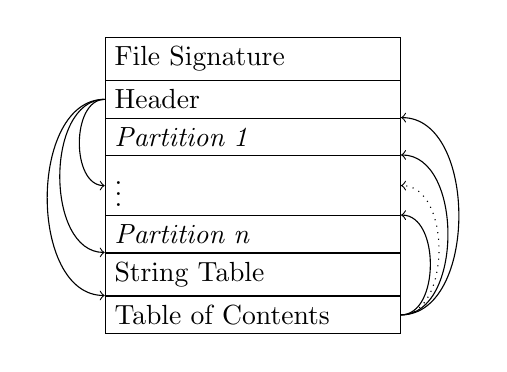
\begin{tikzpicture}
    \matrix (ifc) [matrix of nodes,
            row sep=-\pgflinewidth,
            nodes={rectangle,draw,anchor=west,text width=10em}]
    {
      {File Signature} \\
      {Header} \\
      \textit{Partition 1} \\
      $\vdots$ \\
      \textit{Partition n} \\
	{String Table} \\
      {Table of Contents}\\
    };
	%% Header gives offsets to ToC, String Table, Global Scope.
	\draw [->] (ifc-2-1.west) to [out=180,in=180] (ifc-7-1.north west);
	\draw [->] (ifc-2-1.west) to [out=180,in=180] (ifc-6-1.north west);
	\draw [->] (ifc-2-1.west) to [out=180,in=180] (ifc-4-1.west);

	\draw[->] (ifc-7-1.east) to [out=0,in=0] (ifc-3-1.north east);
	\draw[->] (ifc-7-1.east) to [out=0,in=0] (ifc-4-1.north east);
	\draw[dotted,->] (ifc-7-1.east) to [out=0,in=0] (ifc-4-1.east);
	\draw[->] (ifc-7-1.east) to [out=0,in=0] (ifc-5-1.north east);
  \end{tikzpicture}
  \caption{IFC file general structure}
  \label{fig:ifc-file-overview}
\end{figure}

\noindent
An IFC represents the \emph{abstract semantics graph} that is the result
of elaborating declarations in an input source file, e.g. a module interface file,
 or a header unit, or indeed any C++ source file that leads to a 
well-formed translation unit.
Declarations and expressions are designated by \emph{abstract references}.  An
abstract reference is essentially a typed pointer that refers to an index in a
partition.  The specific partition is given by the \field{tag} field of the abstract
reference, and the index is given by the \term{index} field of the reference.  All
abstract references are multiple-byte values with 32-bit precision:
%
\begin{figure}[H]
  \centering
	\begin{BasicAbstractReferenceLayout}{32}
		\bitfield{10}{\field{tag}: \clipType{Sort}{N}}
      		\bitfield{22}{\field{index}: \clipType{Index}{32 - N} }
		\bitFormatTextAt{N-1}{8}
 		\bitSeparate{10}
		\bitFormatTextAt{N}{10}
	\end{BasicAbstractReferenceLayout} 
  \caption{Abstract reference parameterized by the sort of designated entity.}
  \label{fig:ifc-abstract-reference}
\end{figure}
%

\noindent
The overall aim is to define the binary representations after the 
\emph{Internal Program Representation} (IPR), a work done by Gabriel Dos~Reis
and Bjarne Stroustrup \cite{gdr-bs:ipr-macis-special-issue,ipr:web} to define a more regular 
foundational semantics for
C++, capable of capturing ISO C++ and practical dialects.

\section{Multiple IFCs per file}
\label{sec:ifc-multiple-ifcs-per-file}

The current specification only defines one IFC per containing file.  However, the long term goal is to support multiple IFCs per containing file.
Where there is a mention of "offset from the beginning of the file", it should be understood "offset from the beginning of the current IFC".

\section{Type of IFC container}
\label{sec:ifc-type-of-ifc-container}

An IFC can be embedded in just any binary file.  The VC++ compiler by default generates IFCs in binary files with the 
\code{.ifc} extension.  However, they can also be embedded in archives (e.g. files with \code{.a} or \code{.lib} extensions), or
in shared or dynamically linked libraries (e.g. files with \code{.so}, \code{.dll}, \code{.dylib} extensions.)

\section{On-demand materialization}

The IFC format is designed to support (and encourage) ``on-demand''
materialization of declarations.  That is, when the compiler sees an
import-declaration, it does \emph{not} bring in all the declarations
right away.  Rather, the idea is that it only makes visible
the set of (toplevel) names exported by the nominated module.  An
on-demand materialization strategy will only reconstruct declarations
upon name lookup (in response to a name use in the importing
translation unit) however referenced.  The on-demand materialization
strategy embodies C++'s long standing philosophy of ``you don't pay
for what you don't use.''

\section{Endianness}
\label{sec:ifc-endianness}

Each multibyte scalar value used in the description of an IFC file header (\secref{sec:ifc-file-header})
and in the table of contents (\secref{sec:ifc-toc})
is stored in little endian format. Multibyte scalar values stored in the partitions use the
endianness of the target architecture.

\section{Basic data types}
\label{sec:ifc-basic-data-types}

This document uses a few fundamental data types, \type{u8}, \type{u16}, and \type{32} with the following characteristics:
\begin{itemize}
	\item \type{u8}: $1$ octet, with alignment $1$; usually equivalent to C++'s \code{uint8_t}
	\item \type{u16}: $2$ octets, with alignment $2$; usually equivalent to C++'s \code{uint16_t}
	\item \type{u32}: $4$ octets, with alignment %4%; usually equivalent to C++'s \code{uint32_t} 
\end{itemize} 

\subsection{File offset in bytes}
At various places, the locations of certain tables (especially partitions) are
described in terms of byte offset from the beginning of the current IFC file.  The
document uses the following abstract data type for those quantities.
\newtype{ByteOffset}{32}

\paragraph{Note:}
The current implementation uses 4-byte for file offsets, but that will change
in coming updates to 8-byte in anticipation of large IFC file support.

\subsection{Cardinality: counting items}
At various places, the IFC indicates how many elements there are in a given
table.  That information is given by a 32-bit integer value abstracted as
follows: \newtype{Cardinality}{32}

\subsection{Extent of entities}
\label{sec:ifc-entity-size}
At various places, in particular in partition summaries (\secref{sec:ifc-partition}), the IFC needs to indicate 
the number of bytes contain in entity representation.  That information is
indicated by a 32-bit value of type \newtype{EntitySize}{32}

\subsection{Generic Indices}
\label{sec:ifc-index-type}
The type of generic indices into tables is defined as \newtype{Index}{32}

\subsection{Sequence}
\label{sec:ifc-sequence}
A sequence is generically described by a pair:
%
\begin{figure}[H]
	\centering
	\structure{
		\DeclareMember{start}{Index} \\
		\DeclareMember{cardinality}{Cardinality}\\
	}
	\caption{Structure of a sequence}
	\label{fig:ifc-sequence-structure}
\end{figure}
%
The \field{start} field is an index into the partition the sequence is part of.  It designates the first item in the sequence.
The \field{cardinality} designates the number of items in the sequence.

\subsection{Content Hash}
\label{sec:content-sha256-hash}
The interesting portion of the content of an IFC file is hashed using SHA-256 algorithm, and stored as a value of type \type{SHA256}:
A basic data type with 256 bits width, and with alignment 4.

\subsection{File Format Versioning}
\label{sec:ifc-versioning-data-type}

Each IFC header has version information, major and minor of type defined as \newtype{Version}{8}

\subsection{ABI}
\label{sec:ifc-abi-data-type}
The ABI targeted by an IFC is recorded in a field of the IFC header, of type \newtype{Abi}{8}

\subsection{Architecture}
\label{sec:ifc-architecture-data-type}
The architecture targeted by an IFC is recorded in a field of the IFC header, of type
\begin{typedef}{Architecture}{}
	enum class Architecture : uint8_t {
		Unknown	= 0x00,		// Unknown target
		X86			= 0x01,		// x86 (32-bit) target
		X64			= 0x02,		// x64 (64-bit) target
		ARM32		= 0x03,		// ARM (32-bit) target
		ARM64		= 0x04,		// ARM (64-bit) target
		HybridX86ARM64 = 0x05,	// Hybrid x86-arm64
	};
\end{typedef}

\subsection{Language Version}
\label{sec:ifc-language-version}

The C++ language version is a 32-bit value of type \newtype{LanguageVersion}{32}

\section{IFC File Signature}
\label{sec:ifc-file-signature}

Each valid IFC file (see \figref{fig:ifc-file-overview}) starts with the following 4-byte file signature:
\begin{lstlisting}
  0x54  0x51 0x45 0x1A
\end{lstlisting}


\section{IFC File Header}
\label{sec:ifc-file-header}

Following the file signature (\secref{sec:ifc-file-signature}) is a header that describes a checksum, 
format version information, ABI information, target architecture information, C++ language version,
 the offset to the string table (\secref{sec:ifc-string-table}) and how long it is, 
the name of the IFC's module, the filename of the original C++ source file, the index of the global scope,
then an indication on
where to find the ``table of contents'' (\secref{sec:ifc-toc}), and finally how many partitions (\secref{sec:ifc-partition})
the IFC contains.
%
\begin{figure}[H]
  \centering
    \structure[text width = 15em]{
	\DeclareMember{checksum}{SHA256} \\
	\DeclareMember{major\_version}{Version} \\
      \DeclareMember{minor\_version}{Version} \\
      \DeclareMember{abi}{Abi} \\
      \DeclareMember{arch}{Architecture} \\
	\DeclareMember{dialect}{LanguageVersion} \\
	\DeclareMember{string\_table\_bytes}{ByteOffset} \\
	\DeclareMember{string\_table\_size}{Cardinality} \\
	\DeclareMember{unit}{UnitIndex} \\
	\DeclareMember{src\_path}{TextOffset} \\
	\DeclareMember{global\_scope}{ScopeIndex} \\
      \DeclareMember{toc}{ByteOffset} \\
	\DeclareMember{partition\_count}{Cardinality} \\
	\DeclareMember{internal}{bool} \\
    }
  \caption{Structure of an IFC binary file header}
  \label{fig:ifc-file-header}
\end{figure}

The interpretation of the fields is as follows:
\begin{description}
\item[Content checksum]
	The field \field{checksum} represents the SHA-256 hash of the portion of the IFC file content starting from right after 
	that field to the end of the IFC file.

\item[Version]
	The fields \field{major\_version} and \field{minor\_version} collectively denote the version of the data structures in the
	IFC. The current format version is $0.25$, meaning \field{major\_version} is $0$,
	and \field{minor\_version} is $25$.

\item[Target ABI] 
	The field \field{abi} records the ABI of the target platform of the IFC.

\item[Target Architecture]
	The field \field{arch} records the architecture targeted by the IFC.

\item[C++ Language Version]
	The field \field{dialect} records the value of the C++ pre-defined macro \code{\_\_cplusplus} in effect
	when the IFC was created.

\item[String Table]
	The field \field{string\_table\_bytes} is an offset from the beginning of the IFC to the first byte of the string table (\secref{sec:ifc-string-table}).
	the number of bytes in table is indicated by \field{string\_table\_size}.

	The string table holds the representation of any single strings or identifiers in the IFC.  Consequently, locating it is
	essential for determining the IFC's module name, and also for locating partitions by name.

\item[Translation Unit Descriptor]
	A classification of the translation unit for which this IFC was generated is described by the field \field{unit},  value of
     type \type{UnitIndex} (\secref{sec:ifc-tu}).

\item[Source Pathname]
	The filename of the C++ source file out of which the IFC was produced is indicated by the field \field{src\_path}, an
	offset into the string table.  In the current implementation, this is an ordinary NUL-terminated narrow string.

\item[Global Scope]
	Every declaration is rooted in the global namespace.  The field \field{global\_scope} is index into the
	scope partition (\secref{sec:ifc-scope-desc}), pointing to the description of the global namespace.  Traversing the global scope, and recursively any 
	contained declaration, gives the entire abstract semantics graph making up the IFC.

\item[Table of Contents]
	The table of contents is an array of all partition summaries in the IFC.  The field \field{toc} indicates the offset (in bytes)
	from the beginning of the offset to the first partition descriptor.  The number of partition summaries in the table of contents
	is given by the field \field{partition\_count}.

\item[Internal Unit]
	Whether the IFC is for an exported module unit or not is indicated by \field{internal}.  This field is false for all
	translation units are produced except non-exported module partitions.

\end{description}

\paragraph{Note}
The values of the major and minor versions, the ABI, and the architecture fields
are not fixed yet.   All multi-byte integer values in header are stored according to a little endian format.  All multi-byte integer values
stored in the partitions are stored according to the endianness of the target architecture.
The structure of the field {internal} may change in future revisions.


%% \paragraph{ToC offset}
%% The offset to the table of contents is currently
%% encoded over 4 bytes, but that may change soon to 8 bytes.  
%% This field
%% indicates the relative position (in bytes) of the \code{TableOfContents} from
%% the beginning of the IFC file.

\section{IFC Table of Contents}
\label{sec:ifc-toc}

The data in an IFC are essentially homogenous tables (called
\emph{partitions}) with entries referencing each other.  

The table of 
contents is written near the end of the IFC file as that arrangement
allows one-pass algorithms for writing out IFC files while minimizing
the amount of intermediary internal storage needed to compute the full
abstract semantics graph.

\subsection{Partition}
\label{sec:ifc-partition}

Each partition is described by a \emph{partition summary} information with the
following layout
\begin{figure}[H]
  \centering
  \structure{
      \DeclareMember{name}{TextOffset} \\
      \DeclareMember{offset}{ByteOffset} \\
      \DeclareMember{cardinality}{Cardinality} \\
      \DeclareMember{entry\_size}{EntitySize} \\
    }
  \caption{Partition summary}
  \label{fig:ifc-partition-summary}
\end{figure}

\begin{description}
\item[name] An index into the string pool.  It points to the name (a
  NUL-terminated character string) of the partition.

\item[offset] Location (file offset in bytes) of the partition relative to the
  beginning of the IFC file.

\item[cardinality] The number of items in the partition.

\item[entry\_size] The (common) size of an item in the partition.
\end{description}

So, the byte count of a partition is obtained by multiplying the individual
\field{entry\_size} by the \field{cardinality}.

\section{Elaboration vs. syntax tree}
\label{sec:ifc-elaboration-vs-syntax-tree}

The IFC, like the IPR, is designed to represent all of C++, including extensions.  This means representing faithfully
non-template entities as well as template entities.  An \term{elaboration} of an entity is the result of full semantics
analysis (e.g. the result of name lookup, type checking, overload resolution, template specialization if needed, etc.) of that
entity.  A node, in the abstract semantics graph of an IFC, representing a non-template is an elaboration.

By contrast, semantics analysis of templates proceeds in two steps, by language definition.  For example, in a template code where \code{T} is a type parameter, the meaning of the expression \code{T\{ 42 \}} depends both on the meaning and structure of the 
actual argument value for \code{T}.  It could be a constructor invocation, or a conversion function call, or a non-narrowing
static cast.  Consequently, representations of templates need to be fairly syntactic since only instantiations are fully semantically
analyzed.  Syntax trees (\secref{sec:ifc-syntax-tree-table}) are used to represent templates. 
That representation occasionally contains nodes that are
elaborations, since a certain amount of semantics analysis is required when parsing template definitions.



\chapter{String table}
\label{sec:ifc-string-table}

Every IFC has a string table, a contiguous sequence of bytes.   A regular C++ identifier is stored in the string table as
a NUL-terminated sequence of bytes.

\section{Index type}
\label{sec:ifc-textoffset-data-type}

The type of the indices used to index into the  string table is defined as follows \newtype{TextOffset}{32}

The representation of identifiers  referenced by \type{TextOffset} indices  uses UTF-8 encoding and are NUL-terminated. 
 For string literals, see \secref{sec:ifc:ExprSort:String}.


\chapter{Translation Units}
\label{sec:ifc-tu}

Any C++ translation unit can be compiled into an IFC structure.  A translation unit so represented can be referenced by abstract reference
of type \type{UnitIndex}.  
%
\begin{figure}[htbp]
	\centering
	\absref{3}{UnitSort}
	\caption{\code{UnitIndex}: Abstract reference of a declaration}
	\label{fig:ifc-unit-index}
\end{figure}

\begin{SortEnum}{UnitSort}
	\enumerator{Source}
	\enumerator{Primary}
	\enumerator{Partition}
	\enumerator{Header}
	\enumerator{ExportedTU}
\end{SortEnum}

with meaning as explained in the sections below.  The \field{index} value has a tag-dependent interpretation as defined below.

\section{Translation unit structures}
\label{sec:ifc:tu-structures}

\subsection{\valueTag{UnitSort::Source}}
\label{sec:ifc:UnitSort:Source}
A \type{UnitIndex} value with this tag designates a translation unit defined by a general C++ source file.

The \field{index} value is undefined and has no meaning.


\subsection{\valueTag{UnitSort::Primary}}
\label{sec:ifc:UnitSort:Primary}

A \type{UnitIndex} value with this tag designates a primary module interface.

The \field{index} is to be interpreted as a \type{TextOffset} value (\secref{sec:ifc-textoffset-data-type}), 
which is an offset into the string table (\secref{sec:ifc-string-table}).  
The string at that offset is the name of the module (\secref{sec:ifc-modules}) for which this translation unit is a primary module interface.


\subsection{\valueTag{UnitSort::Partition}}
\label{sec:ifc:UnitSort:Partition}

A \type{UnitIndex} value with this tag designates a partition module unit.

The \field{index} is to be interpreted as a \type{TextOffset} value that designates the name of the module partition.  
The string of that name is \texttt{M:P}, obtained as the concatenation of the name \texttt{M} of the parent module, 
the colon character (\texttt{:}), and the relative name \texttt{P} of the partition.

\subsection{\valueTag{UnitSort::Header}}
\label{sec:ifc:UnitSort:Header}

A \type{UnitIndex} value with this tag designates a C++ header unit.  The \field{index} value is undefined and has no meaning.


\subsection{\valueTag{UnitSort::ExportedTU}}
\label{sec:ifc:UnitSort:ExportedTU}

A \type{UnitIndex} value with this tag designates a translation unit compiled by the MSVC compiler with the compiler flags
\texttt{/module:export} and \texttt{/module:name}.  Such a translation is processed as if every toplevel declaration was
prefixed with the keyword \texttt{export}.  This is an MSVC extension.

The \field{index} is to be interpreted as a \type{TextOffset} value that designates the name specified via the compiler
switch \texttt{/module:name}.

\note{An IFC unit of this sort is deprecated and scheduled for removal from MSVC.}



\chapter{Modules}
\label{sec:ifc-modules}

Any translation unit can import any module.  Additionally, a module interface can re-export an imported module.

\section{Module description structures}
\label{sec:ifc:module-structures}

\subsection{Module reference}
\label{sec:ifc--module-reference}

All used modules (whether imported or exported) are represented as module references of type defined as follows
%
\begin{figure}[h]
	\centering
	\structure{
		\DeclareMember{owner}{TextOffset} \\
		\DeclareMember{partition}{TextOffset} \\
	}
	\caption{Structure of a \type{ModuleReference}}
	\label{fig:ifc-module-reference-structure}
\end{figure}
%

The fields of a module references have the following meanings:
\begin{itemize}
	\item[owner] This value designates the name of the module.  A null name indicated the global module.

	\item[partition] This value designates the partition of the owning module.  When the partition name is null, the reference is to
	the primary module interface, otherwise it designates the partition of the owning module.  When the owner is the global module
	then the partition designates the source file representing that partition of the global module.
\end{itemize}


\subsection{Imported modules}
\label{sec:ifc-imported-module}

References to all imported modules (which are not also exported) are stored in the imported modules partition.

\partition{module.imported}


\subsection{Exported modules}
\label{sec:ifc-exported-module}

References to all exported modules are stored in the exported modules partition.

\partition{module.exported}


\chapter{Scopes}
\label{sec:ifc-scopes}

Every non-empty C++ translation unit contains at least one declaration, reachable from the global scope.

\section{Scope index}
\label{sec:ifc-scope-index}

A scope is referenced via an abstract reference of type \type{ScopeIndex} defined as \newtype{ScopeIndex}{32}
%
A value of type \type{ScopeIndex} is an index into the scope partition described below.  Valid values start at 1.  A \type{ScopeIndex} value 0 
indicates a missing scope, not an empty scope.

\section{Scope descriptor}
\label{sec:ifc-scope-desc}

A scope is a sequence of declarations (\secref{sec:ifc-scope-member}) -- this definition is a generalization of standard C++'s.
%
\begin{figure}[h]
	\centering
	\structure{
		\DeclareMember{start}{Index} \\
		\DeclareMember{cardinality}{Cardinality} \\
	}
	\caption{Structure of a \type{Scope}}
	\label{fig:ifc-scope-structure}
\end{figure}
%
The \field{start} is an index into the scope member partition (\secref{sec:ifc-scope-member}), designating the first declaration in the scope.
The \field{cardinality} designates the number of declarations in the scope.  Only members declared in that scope from that module partition
are accounted for in the scope descriptor.

\partition{scope.desc}

\note{The \field{global\_scope} field of the table of contents (\secref{sec:ifc-file-header}) is index into this partition.}

\section{Scope member}
\label{sec:ifc-scope-member}

A scope member represents a declaration.
%
\begin{figure}[h]
	\centering
	\structure{
		\DeclareMember{index}{DeclIndex} \\
	}
	\caption{Structure of a \type{Declarataion} -- a scope member}
	\label{fig:ifc-declaration-structure}
\end{figure}
%

The \field{index} field of a declaration is a \type{DeclIndex} value designating the entity (\secref{sec:ifc-decls}) referenced by this declaration.

\partition{scope.member}

\note{At this point in time, a \type{Declaration} is just a structure with an index as member.  In the future, it may evolve to contain explicitly attributes such as 'imported', 'exported', or 'internal'. }

\chapter{Heaps}
\label{sec:ifc-heaps}

At various places, there is a need to describe a sequence of objects of a given (common) sort but of differing kinds.  
For example, a namespace contains only declarations, but those declarations can be of different kinds; e.g. function declaration, variable declaration,
template declaration, etc.  Those tables are represented as sequences of homogenous indices of one sort: a slice of a heap of indices.

\section{Heap structures}
\label{sec:ifc:heap-structures}

\subsection{Declaration heap}
\label{sec:ifc-decl-heap}

The declarations heap is a partition consisting entirely of \type{DeclIndex} values.

\partition{heap.decl}

\subsection{Directive heap}
\label{sec:ifc-dir-heap}

The directive heap is a partition consisting entirely of \type{DirIndex} values.

\partition{heap.dir}


\subsection{Type heap}
\label{sec:ifc-type-heap}

The types heap is a partition consisting entirely of \type{TypeIndex} values.

\partition{heap.type}


\subsection{Statement heap}
\label{sec:ifc-stmt-heap}

The statement heap is a partition consisting entirely of \type{StmtIndex} values.

\partition{heap.stmt}


\subsection{Expression heap}
\label{sec:ifc-expr-heap}

The expression heap is a partition consisting entirely of \type{ExprIndex} values.

\partition{heap.expr}


\subsection{Syntax heap}
\label{sec:ifc-syntax-heap}

The syntax heap is a partition consisting entirely of \type{SyntaxIndex} values.

\partition{heap.syn}

\subsection{Form heap}
\label{sec:ifc-form-heap}

The preprocessing form heap is a partition consisting entirely of \type{FormIndex} values.

\partition{heap.form}



\subsection{Chart heap}
\label{sec:ifc-chart-heap}

The chart heap is a partition consisting entirely of \type{ChartIndex} values.

\partition{heap.chart}

\subsection{Attribute heap}
\label{sec:ifc-attr-heap}


The attribute heap is a partition consisting entirely of \type{AttrIndex} values.

\partition{heap.attr}


\chapter{Declarations}
\label{sec:ifc-decls}

Declarations are indicated by abstract declaration references.  This document
uses \type{DeclIndex} to designate a typed abstract reference to a
declaration.  Like all abstract references, it is a 32-bit value
\begin{figure}[htbp]
  \centering
  \absref{5}{DeclSort}
  \caption{\type{DeclIndex}: Abstract reference of declaration}
  \label{fig:ifc-decl-index}
\end{figure}

\begin{SortEnum}{DeclSort}
	\enumerator{VendorExtension}
	\enumerator{Enumerator}
	\enumerator{Variable}
	\enumerator{Parameter}
	\enumerator{Field}
	\enumerator{Bitfield}
	\enumerator{Scope}
	\enumerator{Enumeration}
	\enumerator{Alias}
	\enumerator{Temploid}
	\enumerator{Template}
	\enumerator{PartialSpecialization}
	\enumerator{Specialization}
	\enumerator{DefaultArgument}
	\enumerator{Concept}
	\enumerator{Function}
	\enumerator{Method}
	\enumerator{Constructor}
	\enumerator{InheritedConstructor}
	\enumerator{Destructor}
	\enumerator{Reference}
	\enumerator{UsingDeclaration}
	\enumerator{Unused0}
	\enumerator{Friend}
	\enumerator{Expansion}
	\enumerator{DeductionGuide}
	\enumerator{Barren}
	\enumerator{Tuple}
	\enumerator{SyntaxTree}
	\enumerator{Intrinsic}
	\enumerator{Property}
	\enumerator{OutputSegment}
\end{SortEnum}

\paragraph{Note:}
The individual values a \type{DeclSort} enumerator is subject to change
at any moment until the design stabilizes.

\section{Declaration vocabulary types}
\label{sec:ifc-decl-support-types}

The description of declarations uses a set of common types values as described below.

\subsection{Access specifiers}
\label{sec:ifc-access-specifier}

Every non-local declaration has an access specifier, of type:
\begin{typedef}{Access}{}
	enum class Access : uint8_t {
		None,				// No access specifier
		Private,				// "private" for scope member
		Protected,			// "protected" for scope member
		Public,				// "public" for scope member
	};
\end{typedef}

\subsection{Basic specifiers}
\label{sec:ifc-basic-specifiers}

Certain cumulative properties common to all declarations are described by the bitmask type \type{BasicSpecifiers}:
%
\begin{typedef}{BasicSpecifiers}{}
	enum class BasicSpecifiers : uint8_t {
		Cxx                     = 0,        // C++ language linkage
		C                       = 1 << 0,   // C language linkage
		Internal                = 1 << 1,   // 
		Vague                   = 1 << 2,   // Vague linkage, e.g. COMDAT, still external
		External                = 1 << 3,   // External linkage.
		Deprecated              = 1 << 4,   // [[deprecated("foo")]]
		InitializedInClass      = 1 << 5,   // defined or initialized in a class
		NonExported             = 1 << 6,   // Not explicitly exported
		IsMemberOfGlobalModule  = 1 << 7    // member of the global module
	};
\end{typedef}
%

\note{The definition of \type{BasicSpecifiers} may change in the future, and may in fact be part of \type{Declaration} (\secref{sec:ifc-scope-member}).
The numerical values assigned to these symbolic constants are subject to change.
}

\subsection{Reachable semantic properties}
\label{sec:ifc-reachable-properties}

In certain circumstances, the IFC stores more information than the bare minimum
required by the ISO C++ Modules specification.  In such cases, it is necessary to know 
which semantic properties are reachable, outside the owning module, to the importers.
In other circumstances, known such additional information is useful in performing
additional checks such as ODR violation detection.  The availability of such
supplementary information is indicated by the bitmask \type{ReachableProperties}
\begin{typedef}{ReachableProperties}{}
    enum class ReachableProperties : uint8_t {
        None                = 0,        // nothing beyond name, type, scope.
        Initializer         = 1 << 0,   // IPR-initializer exported.
        DefaultArguments    = 1 << 1,   // function or template default arguments exported
        Attributes          = 1 << 2,   // standard attributes exported.
        All                 = 0xff,     // Everything.
    };
\end{typedef}
%



\subsection{Object traits}
\label{sec:ifc-object-traits}

Certain cumulative properties common to all data/object declarations are described by the bitmask type \type{ObjectTraits}
%
\begin{typedef}{ObjectTraits}{}
	enum class ObjectTraits : uint8_t {
		None					= 0,
		Constexpr				= 1 << 0,
		Mutable				= 1 << 1,
		ThreadLocal			= 1 << 2,
		Inline					= 1 << 3,
		InitializerExported	= 1 << 4,
		Vendor					= 1 << 7,
	};
\end{typedef}
%

\note{The definition of \type{ObjectTraits} is subject to change.
The numerical values assigned to these symbolic constants are subject to change.}

\subsection{Vendor traits}
\label{sec:ifc-msvc-trait-bitset}

Declarations of certain entities may be endowed with vendor-specific traits.
The MSVC-specific traits are defined by the following enumeration
\begin{typedef}{MsvcTraits}{}
	enum class MsvcTraits : uint32_t {
		None					= 0,
		ForceInline			= 1 << 0,
		Naked					= 1 << 1,
		NoAlias				= 1 << 2,
		NoInline				= 1 << 3,
		Restrict				= 1 << 4,
		SafeBuffers			= 1 << 5,
		DllExport				= 1 << 6,
		DllImport				= 1 << 7,
		CodeSegment			= 1 << 8,
		Novtable				= 1 << 9,
		IntrinsicType			= 1 << 10,
		EmptyBases			= 1 << 11,
		Process				= 1 << 12,
		Allocate				= 1 << 13,
		SelectAny				= 1 << 14,
		Comdat				= 1 << 15,
		Uuid					= 1 << 16,
	};
\end{typedef}

\subsection{Parameter Level}

A template declaration can have many nesting levels.  This is the case of member templates of class templates; that is a member of a class template, that is itself a template.
Parameter nesting level starts from 1.  The nesting level is given by a value of type \type{ParameterLevel} defined as
\newtype{ParameterLevel}{32}

\subsection{Parameter Position}

A parameter at a given level can be identified by its position in its enclosing parameter list.  The  position of a template parameter is given by a value of type \type{ParameterPosition}, defined as \newtype{ParameterPosition}{32}

\section{Declaration structures}
\label{sec:ifc:decl-structures}

\subsection{\valueTag{DeclSort::VendorExtension}}
\label{sec:ifc:DeclSort:VendorExtension}
A \type{DeclIndex} value with tag \valueTag{DeclSort::VendorExtension} represents an abstract reference to a vendor-specific declaration.
This tag value is reserved for encoding vendor-specific extensions.

\partition{decl.vendor-extension}

\subsection{\valueTag{DeclSort::Enumerator}}
\label{sec:ifc:DeclSort:Enumerator}

A \type{DeclIndex} value with tag \valueTag{DeclSort::Enumerator} represents
an abstract reference to an enumerator declaration.
The \field{index} field is an index into the enumerator declaration partition.
Each entry in that partition is a structure with the following components:
a \field{name} field, a \field{locus} field, a \field{type} field, an \field{initializer} field,
a \field{specifier} field, and an \field{access} field.
%
\begin{figure}[H]
	\centering
	\structure{
		\DeclareMember{name}{TextOffset} \\
		\DeclareMember{locus}{SourceLocation} \\
		\DeclareMember{type}{TypeIndex} \\
		\DeclareMember{initializer}{ExprIndex} \\
		\DeclareMember{specifier}{BasicSpecifiers} \\
		\DeclareMember{access}{Access} \\
	}
	\caption{Structure of an enumerator declaration}
	\label{fig:ifc-enumerator-decl-structure}
\end{figure}
%
The \field{name} field denotes the C++ source-level name of the enumerator.
The \field{locus} field denotes the source location.
The \field{type} field denotes the type of the enumerator.
The \field{initializer} field denotes the value or the initializer of the enumerator.
The \field{specifier} field denotes the specifiers of the enumerator.
The \field{access} field denotes the C++ source-level access specifier of the enumerator.

\partition{decl.enumerator}

\subsection{\valueTag{DeclSort::Variable}} 
\label{sec:ifc:DeclSort:Variable}

A \type{DeclIndex} value with tag \valueTag{DeclSort::Variable} represents an abstract
reference to a variable declaration.  Note that static data members are also
semantically variables and are represented as such.
The \field{index} field is an index into the variable declaration partition.
Each entry in that partition is a structure with the following components:
a \field{name} field, a \field{locus} field, a \type{field}, a \field{home\_scope} field,
an \field{initializer} field, an \field{alignment} field, a \field{specifier} field, a \field{traits}
field, and an \field{access} field.
%
\begin{figure}[H]
	\centering
	\structure[text width = 14em]{
		\DeclareMember{name}{NameIndex} \\
		\DeclareMember{locus}{SourceLocation} \\
		\DeclareMember{type}{TypeIndex} \\
		\DeclareMember{home\_scope}{DeclIndex} \\
		\DeclareMember{initializer}{ExprIndex} \\
		\DeclareMember{alignment}{ExprIndex} \\
		\DeclareMember{traits}{ObjectTraits} \\
		\DeclareMember{specifier}{BasicSpecifiers} \\
		\DeclareMember{access}{Access} \\
		\DeclareMember{properties}{ReachableProperties} \\
	}
	\caption{Structure of a variable declaration}
	\label{fig:ifc-variable-decl-structure}
\end{figure}
%
The \field{name} field denotes the name of the variable.  Note that it can be a plain identifier (a \type{TextOffset} into the string table), or something
as elaborated as a template-id (for specializations of variable templates).
The \field{locus} field denotes the source location.
The \field{type} field denotes the C++ source-level type of the variable.
The \field{home\_scope} field denotes the scope declaration that holds the object the variable designates.  The \field{home\_scope} 
is not necessarily the lexical scope of a variable: for instance, a block-scope 'extern' declaration of a variable names a variable whose 
home scope in the nearest enclosing namespace scope.
The \field{initializer} field denotes the initializer expression in the variable declaration.
The \field{alignment} field denotes the alignment of the variable.
The \field{specifier} field denotes the declarations specifiers of the variable.
The \field{traits} field denotes additional traits associated with the variable.
The \field{properties} field indicates which semantic properties are reachable 
to the importers.

\partition{decl.variable}


\subsection{\valueTag{DeclSort::Parameter}}
\label{sec:ifc:DeclSort:Parameter}

A \type{DeclIndex} value with \field{tag} \valueTag{DeclSort::Parameter} is an abstract reference to 
either a function parameter or a template parameter declaration.
The \field{index} field is an index into the parameter declaration partition.  
Each entry in that partition is a structure with the following layout
%
\begin{figure}[H]
	\centering
	\structure[text width = 14em]{
			\DeclareMember{name}{TextOffset} \\
			\DeclareMember{locus}{SourceLocation} \\
			\DeclareMember{type}{TypeIndex} \\
			\DeclareMember{constraint}{ExprIndex} \\
			\DeclareMember{initializer}{ExprIndex} \\
			\DeclareMember{level}{ParameterLevel} \\
			\DeclareMember{position}{ParameterPosition} \\
			\DeclareMember{sort}{ParameterSort} \\
			\DeclareMember{properties}{ReachableProperties} \\
		}
	\caption{Structure of a template parameter declaration}
	\label{fig:ifc-template-parameter-structure}
\end{figure}
%
and these meanings of the fields:
\begin{itemize}
	\item \field{name} denotes the name of the template parameter.  If null, the template parameter was unnamed in the source input.
	\item \field{locus} denotes the location of the template parameter.
	\item \field{type} designates the type of the parameter.
	\item \field{constaint} designates the concept predicate used to declare this parameter, if the abbreviated form was used at the input source level.
	\item \field{initializer} designates the corresponding default argument, if any.
	\item \field{level} denotes the nesting level of this parameter
	\item \field{position} denotes the position of this parameter in the parameter list
	\item \field{sort} denotes the sort of parameter (function-parameter vs template-parameter)
	\item \field{properties} denotes the set of reachable properties of this parameter.
\end{itemize}

If the parameter declaration was that of a pack, then its type is denoted by a pack expansion (\sortref{Expansion}{TypeSort}).

\note{This representation will change in the future as it is currently too irregular and too tightly coupled with VC++ internal representation oddities.}

\partition{decl.parameter}

\subsubsection{Parameter sort}
\label{sec:ifc-parameter-sort}

The various notions of parameters (function parameter, type template parameter, non-type template parameter, template template parameter) are described by:
\begin{typedef}{ParameterSort}{}
	enum class ParameterSort : uint8_t {
		Object,					// Function parameter
		Type,						// Type template parameter
		NonType,					// Non-type template parameter
		Template,					// Template template parameter
	};
\end{typedef}

\subsection{\valueTag{DeclSort::Field}} 
\label{sec:ifc:DeclSort:Field}

A \type{DeclIndex} value with tag \valueTag{DeclSort::Field} represents 
an abstract reference to the representation of a non-static data member declaration.
The \field{index} field is an index into the field declaration partition.
Each entry in that partition is a structure with the following components:
a \field{name} field, a \field{locus} field, a \field{type} field, a \field{home\_scope} field,
an \field{initializer} field, an \field{alignment} field, a \field{specifier} field,
a \field{traits} field, and an \field{access} field.
%
\begin{figure}[H]
	\centering
	\structure[text width = 14em]{
		\DeclareMember{name}{TextOffset} \\
		\DeclareMember{locus}{SourceLocation} \\
		\DeclareMember{type}{TypeIndex} \\
		\DeclareMember{home\_scope}{DeclIndex} \\
		\DeclareMember{initializer}{ExprIndex} \\
		\DeclareMember{alignment}{ExprIndex} \\
		\DeclareMember{traits}{ObjectTraits} \\
		\DeclareMember{specifier}{BasicSpecifiers} \\
		\DeclareMember{access}{Access} \\
		\DeclareMember{properties}{ReachableProperties} \\
	}
	\caption{Structure of a field declaration}
	\label{fig:ifc-field-decl-structure}
\end{figure}
%
The \field{name} field denotes the name of the non-static data member.
The \field{locus} field denotes the source location.
The \field{type} field denotes the C++ source-level type of the non-static data member.
The \field{home\_scope} field denotes the scope declaration that holds the member declaration.  
The \field{initializer} field denotes the initializer expression in the member declaration.
The \field{alignment} field denotes the alignment of the non-static data member.
The \field{specifier} field denotes the declarations specifiers of the non-static data member.
The \field{traits} fields denotes additional traits associated with the non-static data member.


\partition{decl.field}

\subsection{\valueTag{DeclSort::Bitfield}}
\label{sec:ifc:DeclSort:Bitfield}

A \type{DeclIndex} value with tag \valueTag{DeclSort::Bitfield} represents 
an abstract reference to the representation of a bitfield declaration.
The \field{index} field is an index into the bitfield declaration partition.
Each entry in that partition is a structure with the following components:
a \field{name} field, a \field{locus} field, a \field{type} field, a \field{home\_scope} field,
a \field{width} field,
an \field{initializer} field, a \field{specifier} field,
a \field{traits} field, and an \field{access} field.
%
\begin{figure}[H]
	\centering
	\structure[text width = 14em]{
		\DeclareMember{name}{TextOffset} \\
		\DeclareMember{locus}{SourceLocation} \\
		\DeclareMember{type}{TypeIndex} \\
		\DeclareMember{home\_scope}{DeclIndex} \\
		\DeclareMember{width}{ExprIndex} \\
		\DeclareMember{initializer}{ExprIndex} \\
		\DeclareMember{traits}{ObjectTraits} \\
		\DeclareMember{specifier}{BasicSpecifiers} \\
		\DeclareMember{access}{Access} \\
		\DeclareMember{properties}{ReachableProperties} \\
	}
	\caption{Structure of a bitfield declaration}
	\label{fig:ifc-bitfield-decl-structure}
\end{figure}
%
The \field{name} field denotes the name of the bitfield.
The \field{locus} field denotes the source location.
The \field{type} field denotes the C++ source-level type of the bitfield.
The \field{home\_scope} field denotes the scope declaration that holds the bitfield declaration.  
The \field{width} field denotes the number bits specified in the bitfield declaration.
The \field{initializer} field denotes the initializer expression in the bitfield declaration.
The \field{specifier} field denotes the declarations specifiers of the bitfield.
The \field{traits} fields denotes additional traits associated with the bitfield.

\partition{decl.bitfield}

\subsection{\valueTag{DeclSort::Scope}}
\label{sec:ifc:DeclSort:Scope}

A \type{DeclIndex} abstract reference with tag \valueTag{DeclSort::Scope} designates a class-type or a namespace definition.
The \field{index} field of that abstract reference is an index into the scope declaration partition.
Each entry in that partition is a structure with the following components:
%
\begin{figure}[H]
	\centering
	\structure[text width = 14em]{
		\DeclareMember{name}{NameIndex} \\
		\DeclareMember{locus}{SourceLocation} \\
		\DeclareMember{type}{TypeIndex} \\
		\DeclareMember{base}{TypeIndex} \\
		\DeclareMember{initializer}{ScopeIndex} \\
		\DeclareMember{home\_scope}{DeclIndex} \\
		\DeclareMember{alignment}{ExprIndex} \\
		\DeclareMember{pack\_size}{PackSize} \\
		\DeclareMember{specifiers}{BasicSpecifiers} \\
		\DeclareMember{traits}{ScopeTraits} \\
		\DeclareMember{access}{Access} \\
		\DeclareMember{properties}{ReachableProperties} \\
	}
	\caption{Structure of a scope declaration}
	\label{fig:ifc-scope-decl-structure}
\end{figure}


\noindent
The \field{name} field designates the name of the scope.
The \field{locus} field designates the source location.
The \field{type} field indicates the kind (\secref{sec:ifc:TypeSort:Fundamental}) of scope:
\begin{itemize}
  \item \code{TypeBasis::Struct} means the scope was declared as "\code{struct}"
  \item \code{TypeBasis::Class} means the scope was declared as "\code{class}"
  \item \code{TypeBasis::Union} means the scope was declared as "\code{union}"
  \item \code{TypeBasis::Namespace} means the scope was declared as "\code{namespace}"
  \item \code{TypeBasis::Interface} means the scope was declared as "\code{\_\_interface}"
\end{itemize}
Any other value is invalid.

\noindent
The \field{base} field designates the base class(es) in case of inheritance.
The \field{initializer} field designates the body of the scope definition, e.g. the sequence of declarations.  
Note that valid \type{ScopeIndex} values start from 1, and 0 indicates absence of scope, e.g. an incomplete class type.
The \field{home\_scope} field designates the declaration of the enclosing scope.
The \field{alignment} field designates the alignment value of the scope, in case of class-type.
The \field{pack\_size} field designates the packing value applied to the layout of the scope, in case of class-type.
The \field{specifiers} field indicates the (cumulative) basic declaration specifiers that hold for the scope.
The \field{traits} field designates scope-specific properties of the scope.
The \field{access} field designates the access specifier of the scope declaration.
The \field{properties} field designates the set of reachable semantic properties.

\partition{decl.scope}

\subsubsection{Scope traits}
\label{sec:ifc-scope-traits}

Properties specific to scope entities are described by values of the bitmask type \type{ScopeTraits}:
%
\begin{typedef}{ScopeTraits}{}
	enum class ScopeTraits : uint8_t {
		None			= 0,
		Unnamed		= 1 << 0,
		Inline			= 1 << 1,
		InitializerExported	= 1 << 2,
		ClosureType	= 1 << 3,
		Final = 1 << 4,
		Vendor			= 1 << 7,
	};
\end{typedef}
%
with the following meaning:
\begin{itemize}
  \item \code{ScopeTraits::None}: No scope traits.
  \item \code{ScopeTraits::Unnamed}: the scope is unnamed in the input source code.
  \item \code{ScopeTraits::Inline}: valid only for namespaces.  The namespace is declared \code{inline}.
  \item \code{ScopeTraits::InitializedExported}: valid only if the definition of this scope entity is lexically exported, in particular this indicates whether completeness of types is exported.
  \item \code{ScopeTraits::ClosureType}: valid only for class types.  This trait indicates that the scope represents a closure type.
  \item \code{ScopeTraits::Final}: valid only for class types. This trait indicates that the scope is defined \code{final}.
  \item \code{ScopeTraits::Vendor}: valid only if the scope entity has vendor-defined traits.
\end{itemize}

\subsubsection{Class-type layout packing}
\label{sec:ifc-class-layout-packing}

A value of class layout packing is expressed as value of type \type{PackSize} defined as \newtype{PackSize}{16}

\subsection{\valueTag{DeclSort::Enumeration}}
\label{sec:ifc:DeclSort:Enumeration}

A \type{DeclIndex} abstract reference with tag \valueTag{DeclSort::Enumeration} designates an enumeration declaration.
The \field{index} of that abstract reference is an index into the enumeration declaration partition.
Each entry in that partition is a structure with the following components:
%
\begin{figure}[H]
	\centering
	\structure[text width = 14em]{
		\DeclareMember{name}{TextOffset} \\
		\DeclareMember{locus}{SourceLocation} \\
		\DeclareMember{type}{TypeIndex} \\
		\DeclareMember{base}{TypeIndex} \\
		\DeclareMember{initializer}{Sequence} \\
		\DeclareMember{home\_scope}{DeclIndex} \\
		\DeclareMember{alignment}{ExprIndex} \\
		\DeclareMember{specifiers}{BasicSpecifiers} \\
		\DeclareMember{access}{Access} \\
		\DeclareMember{properties}{ReachableProperties} \\
	}
	\caption{Structure of an enumeration declaration}
	\label{fig:ifc-enumeration-decl-structure}
\end{figure}
%
The \field{name} field designates the name of the enumeration type.
The \field{locus} field designates the source location.
The \field{type} field designates the kind of enumeration, with:
\begin{itemize}
   \item \code{TypeBasis::Enum} meaning a classic enumeration
   \item \code{TypeBasis::Class} or \code{TypeBasis::Struct} meaning a scoped enumeration
\end{itemize}
The \field{base} field designates the underlying type of the enumeration.
The \field{initializer} is a slice (\secref{sec:ifc-sequence}) of the enumerator partition (\secref{sec:ifc:DeclSort:Enumerator}). 
 It designates the sequence of enumerators (if any) declared as part
of the enumeration declaration.
The \field{home\_scope} field designates the declaration of the enclosing scope of the enumeration.
The \field{alignment} designates the alignment specified in the declaration.  A non-zero value indicates an explicit alignment specification
in the input source code.
The \field{specifiers} designates the basic generic declaration specifiers of the enumeration.
The \field{access} designates the access specifier.
The \field{properties} designates the set of reachable semantic properties.

\partition{decl.enum}

\subsection{\valueTag{DeclSort::Alias}} 
\label{sec:ifc:DeclSort:Alias}

A \type{DeclIndex} abstract reference with tag \valueTag{DeclSort::Alias} designates a type alias declaration.
The \field{index} field of that reference is an index into the type alias declaration partition.
Each entry in that partition is a structure with the following components:
%
\begin{figure}[H]
	\centering
	\structure{
		\DeclareMember{name}{TextOffset} \\
		\DeclareMember{locus}{SourceLocation} \\
		\DeclareMember{type}{TypeIndex} \\
		\DeclareMember{home\_scope}{DeclIndex} \\
		\DeclareMember{aliasee}{TypeIndex} \\
		\DeclareMember{specifiers}{BasicSpecifiers} \\
		\DeclareMember{access}{Access} \\
	}
	\caption{Structure of a type alias declaration}
	\label{fig:ifc-type-alias-decl-structure}
\end{figure}
%
\begin{itemize}
	\item The \field{name} field designates the name of the alias.
	\item The \field{locus} field designates the source location.
	\item The \field{type} field denotes the kind of alias: it denotes \code{TypeBasis::Typename} for type aliases; it will be \code{TypeBasis::Namespace} for namespace aliases; it is abstract reference of sort \valueTag{TypeSort::Forall} for template aliases.
	\item The \field{home\_scope} field designates the declaration of the enclosing scope.
	\item The \field{aliasee} field designates the type the alias is declared for.
	\item The \field{specifiers} field designates the basic declaration specifiers for the alias.
	\item The \field{access} field designates the access specifier for the alias.
\end{itemize}

This structure is also used to represent template aliases -- mistakenly called alias templates in the ISO C++ document.  For template aliases,
the \field{aliasee} field denotes a \valueTag{TypeSort::Forall} type (\sortref{Forall}{TypeSort}), which is the representation of the \grammar{template-parameter} list followed by the \grammar{type-id} 
that would syntactically appear on the right hand side of the source-level \grammar{using-declaration}.


\partition{decl.alias}


\subsection{\valueTag{DeclSort::Temploid}}
\label{sec:ifc:DeclSort:Temploid}

A member of a parameterized scope -- does not have template parameters of its own.
%
\begin{figure}[H]
	\centering
	\structure[text width = 14em]{
		\DeclareMember{entity}{ParameterizedEntity}\\
		\DeclareMember{chart}{ChartIndex}\\
		\DeclareMember{properties}{ReachableProperties} \\
	}
	\caption{Structure of a templated declaration}
	\label{fig:ifc-type-temploid-structure}
\end{figure}
%
The \field{entity} field represents the declaration being parameterized.
The \field{chart} field designates the set of template parameter lists of the enclosing scope.
The \field{properties} field designates the set of reachable semantics properties.


\partition{decl.temploid}

\subsubsection{Parameterized Entity}
\label{sec:ifc-parameterized-entity}

The structure \type{ParameterizedEntity} has the following layout
%
\begin{figure}[H]
	\centering
	\structure{
		\DeclareMember{decl}{DeclIndex} \\
		\DeclareMember{head}{SentenceIndex} \\
		\DeclareMember{body}{SentenceIndex} \\
		\DeclareMember{attributes}{SentenceIndex} \\
	}
	\caption{Structure of a declaration parameterized by a template}
	\label{fig:ifc-parameterized-decl-structure}
\end{figure}
%
The \field{decl} field denotes the declaration that is being 
parameterized either directly or indirectly by a set of template parameter lists.
The \field{head} field designates the sentence (\secref{sec:ifc-sentence}) that makes up the
non-defining declarative part of the current instantiation.
That sentence is no longer meaningful in recent releases of MSVC since
any semantics information can be obtained from the entity denoted
by \field{decl}.
The \field{body} field denotes the sentence of the defining ("body") part
of the current instantiation.  This field is meaningful only
for templated functions. 


\subsection{\valueTag{DeclSort::Template}}
\label{sec:ifc:DeclSort:Template}

A template declaration: class, function, constructor, type alias, variable.

\begin{figure}[H]
	\centering
	\structure[text width = 14em]{
		\DeclareMember{name}{NameIndex} \\
		\DeclareMember{locus}{SourceLocation} \\
		\DeclareMember{home\_scope}{DeclIndex} \\
		\DeclareMember{chart}{ChartIndex} \\
		\DeclareMember{entity}{ParameterizedEntity} \\
		\DeclareMember{type}{TypeIndex} \\
		\DeclareMember{specifiers}{BasicSpecifiers} \\
		\DeclareMember{access}{Access} \\
		\DeclareMember{properties}{ReachableProperties} \\
	}
	\caption{Structure of a template declaration}
	\label{fig:ifc-template-decl-structure}
\end{figure}

The \field{name} field denotes the name of this template.
The \field{locus} field denotes the source location of this declaration.
The \field{home\_scope} field designate the home scope of this template.
The \field{chart} field denotes the set of parameter list to this template.
The \field{entity} field describes the declaration being parameterized by this template.  Its structure is defined below.
The \field{type} field denotes the type of this template declaration.
The \field{specifiers} field denotes declaration specifiers for this template.
The \field{access} field denotes the access level of this declaration.
The \field{properties} field designates the set of reachable semantic properties.

\partition{decl.template}

\subsection{\valueTag{DeclSort::PartialSpecialization}}
\label{sec:ifc:DeclSort:PartialSpecialization}

A partial specialization of a
template (class-type or function). 

%
\begin{figure}[H]
	\centering
	\structure[text width = 14em]{
		\DeclareMember{name}{NameIndex} \\
		\DeclareMember{locus}{SourceLocation} \\
		\DeclareMember{home\_scope}{DeclIndex} \\
		\DeclareMember{chart}{ChartIndex} \\
		\DeclareMember{entity}{ParameterizedEntity} \\
		\DeclareMember{form}{Index} \\
		\DeclareMember{specifiers}{BasicSpecifiers} \\
		\DeclareMember{access}{Access} \\
		\DeclareMember{properties}{ReachableProperties} \\
	}
	\caption{Structure of a partial specialization declaration}
	\label{fig:ifc-partial-specialization-decl-structure}
\end{figure}

The \field{name} field denotes the name of the current instantiation of the partial specialization.
The \field{locus} field denotes the source location.
The \field{home\_scope} field denotes the parent declaration of this partial specialization.
The \field{chart} field denotes the set of template-parameter lists of this partial specialization.
The \field{entity} field describes the current instantiation of this partial specialization.
The \field{form} field is an index into the partition of specialization form (template and template-argument list) named \code{"form.spec"}.
The \field{specifiers} field denotes the declaration specifiers of this partial specialization.
The \field{access} field denotes the access level of this partial specialization.
The \field{properties} field denotes the set of reachable semantic properties.

\partition{decl.partial-specialization}

\note{Future revision will represent partial a specialization as a directive.}


\subsection{\valueTag{DeclSort::Specialization}} 
\label{sec:ifc:DeclSort:Specialization}

A \type{DeclIndex} value with tag \valueTag{DeclSort::Specialization} designates a specialization of template declaration.
The \field{index} field of that abstract reference is an index into the specialization partition.
Each entry in that partition is a structure with the following layout
%
\begin{figure}[H]
	\centering
	\structure[text width = 14em]{
		\DeclareMember{form}{Index} \\
		\DeclareMember{decl}{DeclIndex} \\
		\DeclareMember{sort}{SpecializationSort} \\
	}
	\caption{Structure of a template declaration specialization}
	\label{fig:ifc-specialization-declaration}
\end{figure}
%
and meanings of the fields
\begin{itemize}
	\item The value of \field{form} is an index into the specialization form partition (named "form.spec").
	\item \field{decl}, when non null, denotes the declaration produced by the specialization.
	\item \field{sort} designates how the specialization is obtained (\secref{sec:ifc-SpecializationSort}).
\end{itemize}

\partition{decl.specialization}

\subsubsection{How to specialize a template}
\label{sec:ifc-SpecializationSort}

The method by which the declaration for a template specialization is produced can be indicated by a value of type
%
\begin{typedef}{SpecializationSort}{}
	enum class SpecializationSort : uint8_t {
		Implicit = 0x0,
		Explicit = 0x1,
		Instantiation = 0x2,
	};
\end{typedef}
%
with the following meaning
\begin{itemize}
	\item \valueTag{SpecializationSort::Implicit}: the declaration is an implicit specialization.
	\item \valueTag{Specialization::Explicit}: the declaration is an explicit specialization.
	\item \valueTag{Specialization::Instantiation}: the declaration is an explicit instantiation.
\end{itemize}


\subsection{\valueTag{DeclSort::DefaultArgument}} 
\label{sec:ifc:DeclSort:DefaultArgument}

A \type{DeclIndex} value with tag \valueTag{DeclSort::DefaultArgument} represents an abstract reference
to a default argument for a function parameter or a template parameter.  For all practical purposes (ODR),
a default argument is modelled as a declaration.  
The \field{index} of that abstract reference is an index into the default argument
definition partition.  Each entry in that partition is a structure with the following layout
%
\begin{figure}[H]
	\centering
	\structure{
		\DeclareMember{locus}{SourceLocation} \\
		\DeclareMember{type}{TypeIndex} \\
		\DeclareMember{home\_scope}{DeclIndex} \\
		\DeclareMember{initializer}{ExprIndex} \\
		\DeclareMember{specifiers}{BasicSpecifiers} \\
		\DeclareMember{access}{Access} \\
		\DeclareMember{properties}{ReachableProperties} \\
	}
\end{figure}
%
with the following meanings of the fields:
\begin{itemize}
	\item \field{locus} designates the source location of the default argument
	\item \field{type} designates the type of the parameter corresponding to the default argument
	\item \field{home\_scope} designates the scope where the default parameter is specified
	\item \field{initializer} designates the expression specified in the default argument
	\item \field{specifiers} denotes the basic specifiers of the default arguments
	\item \field{access} denotes the control access of this default argument
	\item \field{properties} denotes the reachable properties associated with the default argument
\end{itemize}

\note{The \field{home\_scope} field is currently null in the current IFC produced by the MSVC toolset.}

\partition{decl.default-arg}

\subsection{\valueTag{DeclSort::Concept}}
\label{sec:ifc:DeclSort:Concept}

A \type{DeclIndex} value with tag \valueTag{DeclSort::Concept} represents an abstract reference
to a concept declaration.  The \field{index} of that abstract reference is an index into the concept
definition partition.  Each entry in that partition is a structure with the following layout
%
\begin{figure}[H]
	\centering
	\structure{
		\DeclareMember{name}{TextOffset} \\
		\DeclareMember{locus}{SourceLocation} \\
		\DeclareMember{home\_scope}{DeclIndex} \\
		\DeclareMember{type}{TypeIndex} \\
		\DeclareMember{chart}{ChartIndex} \\
		\DeclareMember{constraint}{ExprIndex} \\
		\DeclareMember{specifiers}{BasicSpecifiers} \\
		\DeclareMember{access}{Access} \\
		\DeclareMember{head}{SentenceIndex} \\
		\DeclareMember{body}{SentenceIndex} \\
	}
	\caption{Structure of a concept declaration}
	\label{fig:ifc-concept-decl-structure}
\end{figure}
%
and meaning of the fields:
\begin{itemize}
	\item \field{name} designates the name of the concept
	\item \field{locus} designates the source location of the concept definition
	\item \field{home\_scope} designates the declaration of the enclosing scope
	\item \field{type} designates the full type of the concept definition
	\item \field{chart} is the parameter list list to the concept
	\item \field{constraint} is the body of predicate defining the concept
	\item \field{specifiers} is the set of basic declaration specifiers
	\item \field{access} is the access specifier for the concept definition
	\item \field{head} is the sequence of words making up the declarative part of the concept
	\item \field{body} is the sequence of words making up the body of the concept definition
\end{itemize}

\partition{decl.concept}

\note{This representation is subject to change in future releases.}

\subsection{\valueTag{DeclSort::Function}}
\label{sec:ifc:DeclSort:Function}

A \type{DeclIndex} value with tag \valueTag{DeclSort::Function} represents
an abstract reference to a function declaration. Note that a static member function is represented as a function.
The \field{index} field is an index into the function declaration partition.
Each entry in that partition is a structure with the following components:
%
\begin{figure}[H]
	\centering
	\structure [text width = 15em] {
		\DeclareMember{name}{NameIndex} \\
		\DeclareMember{locus}{SourceLocation} \\
		\DeclareMember{type}{TypeIndex} \\
		\DeclareMember{home\_scope}{DeclIndex} \\
		\DeclareMember{chart}{ChartIndex} \\
		\DeclareMember{traits}{FunctionTraits} \\
		\DeclareMember{specifiers}{BasicSpecifiers} \\
		\DeclareMember{access}{Access} \\
		\DeclareMember{properties}{ReachableProperties} \\
	}
	\caption{Structure of a function declaration}
	\label{fig:ifc-function-decl-structure}
\end{figure}
%
The \field{name} field designates the name of the function.
The \field{locus} field designates the source location.
The \field{type} field designates the type of the function, including the noexcept-specification (which is now part of the type of a function in C++17).
The \field{home\_scope} denotes the enclosing scope of the function. This may not be the lexical scope of the declaration.
The \field{chart} denotes the chart (\secref{sec:ifc-charts}) of the function parameter list along with their default arguments.  These parameters may be unnamed.
The \field{specifier} denotes basic declaration specifiers; the \field{traits} field adds additional function traits.
Finally, the \field{access} denotes the access specifier for the function.

\note{The set of parameter declarations in a function definition is listed in a separate trait (\secref{sec:ifc-msvc-fun-parms}).  That representation is subject to removal in future MSVC releases.}

\partition{decl.function}

\subsubsection{Function traits}
\label{sec:ifc-function-traits}

Certain function-specific cumulative properties are expressed as values of the bitmask type \type{FunctionTraits} defined as
%
\begin{typedef}{FunctionTraits}{}
	enum class FunctionTraits : uint16_t {
		None			= 0,
		Inline			= 1 << 0,
		Constexpr		= 1 << 1,
		Explicit		= 1 << 2,
		Virtual			= 1 << 3,
		NoReturn		= 1 << 4,
		PureVirtual	= 1 << 5,
		HiddenFriend	= 1 << 6,
		Defaulted		= 1 << 7,
		Deleted		= 1 << 8,
		Constrained   = 1 << 9,
		Immediate = 1 << 10,
		Vendor			= 1 << 15,
	};
\end{typedef}
%
with the following meaning
\begin{description}
	\item \code{FunctionTraits::None}: no property
	\item \code{FunctionTraits::Inline}: the function is declared \code{inline}
	\item \code{FunctionTraits::Constexpr}: the function is declared \code{constexpr}
	\item \code{FunctionTraits::Explicit}: the function is declared \code{explicit}
	\item \code{FunctionTraits::Virtual}: the function is declared \code{virtual}
	\item \code{FunctionTraits::NoReturn}: the function is declared \code{[[noreturn]]} or \code{\_\_declspec(noreturn)}
	\item \code{FunctionTraits::PureVirtual}: the function is pure virtual, e.g. with \code{ = 0}
	\item \code{FunctionTraits::HiddenFriend}: the function is a hidden friend
     \item \code{FunctionTraits::Constrained} : the function has requires-constraints
     \item \code{FunctionTraits::Immediate}: the function is a \code{consteval}, or an immediate function. 
     \item \code{FunctionTraits::Vendor}: the function has vendor-defined traits stored in the
	 MSVC vendor-specific traits (\secref{sec:ifc-msvc-vendor-specific-trait}).
\end{description}


\subsection{\valueTag{DeclSort::Method}} 
\label{sec:ifc:DeclSort:Method}

A \type{DeclIndex} abstract reference with tag \code{DeclSort::Method} designates a non-static member function (which is neither a constructor nor a destructor) declaration.
The \field{index} of that abstract reference is an index into the non-static member function declaration partition.
Each entry in that partition is a structure with the following components
%
\begin{figure}[H]
	\centering
	\structure[text width = 15em]{
		\DeclareMember{name}{NameIndex} \\
		\DeclareMember{locus}{SourceLocation} \\
		\DeclareMember{type}{TypeIndex} \\
		\DeclareMember{home\_scope}{DeclIndex} \\
		\DeclareMember{chart}{ChartIndex} \\
		\DeclareMember{traits}{FunctionTraits} \\
		\DeclareMember{specifiers}{BasicSpecifiers} \\
		\DeclareMember{access}{Access} \\
		\DeclareMember{properties}{ReachableProperties} \\
	}
	\caption{Structure of a non-static member function declaration}
	\label{fig:ifc-method-decl-structure}
\end{figure}
%
The \field{name} field designates the name of the non-static member function.
The \field{locus} field designates the source location of this declaration.
The \field{type} field designates the type of this non-static member function.  Note that the type also includes the calling convention.
The \field{home\_scope} designates the enclosing type declaration.
The \field{chart} designates the function parameter list along with their default arguments.
The \field{traits} indicates any additional function-specific traits (\secref{sec:ifc-function-traits}).
The \field{access} designates the access specifier for this function.

\partition{decl.method}


\subsection{\valueTag{DeclSort::Constructor}} 
\label{sec:ifc:DeclSort:Constructor}

A \type{DeclIndex} abstract reference with tag \valueTag{DeclSort::Constructor} designates a constructor declaration.
The \field{index} field of that abstract reference is an index into the constructor declaration partition.
Each entry in that partition is a structure with the following components.
%
\begin{figure}[H]
	\centering
	\structure[text width = 15em]{
		\DeclareMember{name}{TextOffset} \\
		\DeclareMember{locus}{SourceLocation} \\
		\DeclareMember{type}{TypeIndex} \\
		\DeclareMember{home\_scope}{DeclIndex} \\
		\DeclareMember{chart}{ChartIndex} \\
		\DeclareMember{traits}{FunctionTraits} \\
		\DeclareMember{specifiers}{BasicSpecifiers} \\
		\DeclareMember{access}{Access} \\
		\DeclareMember{properties}{ReachableProperties} \\
	}
	\caption{Structure of a constructor declaration}
	\label{fig:ifc-constructor-decl-structure}
\end{figure}
%
The meaning of the fields is as follows:
\begin{itemize}
	\item \field{name} designates the name of the constructor.
	\item \field{locus} denotes the source location of the constructor.
	\item \field{type} denotes the type of this constructor, a type described in \sortref{Tor}{TypeSort}.
	\item \field{home\_scope} denotes the declaration of the enclosing type.
	\item \field{chart} denotes the function parameter list along with their default argument expressions.
	\item \field{traits} designates function-specific traits (\secref{sec:ifc-function-traits}).
	\item \field{specifiers} designate the usual basic declaration specifiers.
	\item \field{access} designates the access specifier of the constructor.
	\item \field{properties} denotes the set of reachable semantic properties of this constructor declaration.
\end{itemize}

\partition{decl.constructor}

\note{The \field{name} field is subject of further design modification}

The structure \type{NoexceptSpecification} has the following layout
%
\begin{figure}[H]
	\centering
	\structure[text width = 15em]{
		\DeclareMember{words}{SentenceIndex} \\
		\DeclareMember{sort}{NoexceptSort} \\
	}
	\caption{Structure of a \code{noexcept}-specification}
	\label{fig:ifc-noexcept-specification-structure}
\end{figure}
%
The \field{words} field denotes the sentence making up the syntax of the noexcept-specification.
This field is meaningful only for templated functions for which the noexcept-specification is a dependent expression.
The \field{sort} field describes the computed semantics, if not dependent.
It has type
\begin{typedef}{NoexceptSort}{}
	enum class NoexceptSort : uint8_t {
		None,
		False,
		True,
		Expression,
		Inferred,
		Unenforced,
	};
\end{typedef}
with the following meaning
\begin{itemize}
	\item \valueTag{NoexceptSort::None}:  No specification is lexically present in the input source
	\item \valueTag{NoexceptSort::False}: The syntax \code{noexcept(false)} was explicitly used, or the determination has similar semantic effect
	\item \valueTag{NoexceptSort::True}: The syntax \code{noexcept(true)} was explicitly used, or the determination has similar semantic effect.
	\item \valueTag{NoexceptSort::Expression}: The syntax \code{noexcept(expr)} was explicitly used, and no determination could be made because the expression is dependent.
	\item \valueTag{NoexceptSort::Inferred}: The \code{noexcept} specification (for a special member) is inferred and dependent on that of the associated functions
		the special member invokes from base class subobjects or non-static data members. 
	\item \valueTag{NoexceptSort::Unenforced}: This is the specification for the static type system, but with no runtime termination enforcement
\end{itemize}

\subsection{\valueTag{DeclSort::InheritedConstructor}}
\label{sec:ifc:DeclSort:InheritedConstructor}

A \type{DeclIndex} abstract reference with tag \valueTag{DeclSort::InheritedConstructor}
designates an inherited constructor.  The \field{index} of that abstract reference
is an index into the inherited constructor partition.  Each entry in that partition
is a structure with the following layout
%
\begin{figure}[H]
	\centering
	\structure[text width = 15em]{
		\DeclareMember{name}{TextOffset} \\
		\DeclareMember{locus}{SourceLocation} \\
		\DeclareMember{type}{TypeIndex} \\
		\DeclareMember{home\_scope}{DeclIndex} \\
		\DeclareMember{chart}{ChartIndex} \\
		\DeclareMember{traits}{FunctionTraits} \\
		\DeclareMember{specifiers}{BasicSpecifiers} \\
		\DeclareMember{access}{Access} \\
		\DeclareMember{base\_ctor}{DeclIndex} \\
	}
\end{figure}
%
The meaning of the fields is as follows
\begin{itemize}
	\item \field{name} designates the name pf this constructor
	\item \field{locus} denotes the source location of this declaration.
	\item \field{type} denotes the type of this constructor, a type described in \sortref{Tor}{TypeSort}.
	\item \field{home\_scope} denotes the declaration of the enclosing type.
	\item \field{chart} denotes the function parameter list along with their default argument expressions.
	\item \field{traits} designates function-specific traits (\secref{sec:ifc-function-traits}).
	\item \field{specifiers} designate the usual basic declaration specifiers.
	\item \field{access} designates the access specifier of the constructor.
	\item \field{base\_ctor} denotes the constructor from the base class this constructor inherits.
\end{itemize}

\partition{decl.inherited-constructor}

\subsection{\valueTag{DeclSort::Destructor}} 
\label{sec:ifc:DeclSort:Destructor}

 A \type{DeclIndex} abstract reference with tag \valueTag{DeclSort::Destructor} designates a destructor declaration.
The \field{index} field of that abstract reference is an index into the destructor declaration partition.
Each entry in that partition is a structure with the following components.
%
\begin{figure}[H]
	\centering
	\structure[text width = 15em]{
		\DeclareMember{name}{TextOffset} \\
		\DeclareMember{locus}{SourceLocation} \\
		\DeclareMember{home\_scope}{DeclIndex} \\
		\DeclareMember{eh\_spec}{NoexceptSpecification} \\ 
		\DeclareMember{traits}{FunctionTraits} \\
		\DeclareMember{specifiers}{BasicSpecifiers} \\
		\DeclareMember{access}{Access} \\
		\DeclareMember{convention}{CallingConvention} \\
		\DeclareMember{properties}{ReachableProperties} \\
	}
	\caption{Structure of a destructor declaration}
	\label{fig:ifc-destructor-decl-structure}
\end{figure}
%
The \field{name} field designates the name of the destructor declaration.
The \field{locus} field designates the source location of the declaration.
The \field{home\_scope} field designates the declaration of the enclosing type.
The \field{eh\_spec} field designates the exception specification of the declaration.
The \field{traits} field designates function-specific properties (\secref{sec:ifc-function-traits}) of the declaration.
The \field{specifiers} field designate the usual basic declaration specifiers.
The \field{access} field designates the access specifier of the destructor declaration.
The \field{convention} field designates the calling convention used by the destructor.


\note{The \field{name} field is subject of further design modification}


\partition{decl.destructor}


\subsection{\valueTag{DeclSort::Reference}} 
\label{sec:ifc:DeclSort:Reference}

A \type{DeclIndex} abstract reference with tag \valueTag{DeclSort::Reference} designates a reference to a declaration
made available by an imported module.
The \field{index} field of that abstract reference is an index into the declaration reference partition.
Each entry in that partition is a structure with the following components:
%
\begin{figure}[H]
	\centering
	\structure{
		\DeclareMember{unit}{ModuleReference} \\
		\DeclareMember{local\_index}{DeclIndex} \\
	}
	\caption{Structure of a declaration reference declaration}
	\label{fig:ifc-reference-decl-structure}
\end{figure}
%
The \field{unit} field designates the owning translation unit.
The \field{local\_index} is the \type{DeclIndex} abstract reference assigned to that entity by the current (importing) module unit.

\partition{decl.reference}

\subsubsection{\type{ModuleReference}}

The type \type{ModuleReference} is a structure with the following layout
\begin{figure}[H]
	\centering
	\structure{
		\DeclareMember{owner}{TextOffset} \\
		\DeclareMember{partition}{TextOffset} \\
	}
	\caption{Structure of a module reference}
	\label{fig:ifc-module-reference-decl-structure}
\end{figure}

Then the \field{owner} field is null, then it means the IFC comes from the
global module, and the \field{partition} field is the name of the source file
out of which the header unit was built.  Otherwise, \field{owner} is the name
of the owning module of the IFC, and the \field{partition} designates the module
partition when it is not null.

\subsection{\valueTag{DeclSort::UsingDeclaration}} 
\label{sec:ifc:DeclSort:UsingDeclaration}

A \type{DeclIndex} abstract reference with tag \valueTag{DeclSort::UsingDeclaration} designates a using declaration.
The \field{index} field of that abstract reference is an index into the using declaration partition.
Each entry in that partition is a structure with the following components:
%
\begin{figure}[H]
	\centering
	\structure{
		\DeclareMember{name}{NameIndex} \\
		\DeclareMember{locus}{SourceLocation} \\
		\DeclareMember{home\_scope}{DeclIndex} \\
		\DeclareMember{resolution}{DeclIndex} \\
		\DeclareMember{parent}{ExprIndex} \\
		\DeclareMember{name2}{TextOffset} \\
		\DeclareMember{specifiers}{BasicSpecifiers} \\
		\DeclareMember{access}{Access} \\
		\DeclareMember{hidden}{bool} \\
	}
	\caption{Structure of a using-declaration structure}
	\label{fig:ifc-using-declaration-structure}
\end{figure}
%

The \field{name} field is the unqualified part of the using declaration.
The \field{locus} field is the source location of the declaration.
The \field{home\_scope} field designates the enclosing scope of the declaration.
The \field{resolution} field designates the set of used declarations: either a single declaration, or a tuple of declarations.
The \field{parent} field designates the qualifying part of the declaration.
The \field{name2} is a redundant field referring to the name of the member.
The \field{specifiers} field denotes the basic declaration specifiers.
The \field{hidden} field indicates whether the member is hidden.

\partition{decl.using-declaration}

\note{This representation is subject to change.  Future revision will represents this as the result of executing a \grammar{using-declaration} (\sortref{DeclUse}{DirSort}) directive.}


\subsection{\valueTag{DeclSort::Unused0}}
\label{sec:ifc:DeclSort:Unused0}

\diffNote{This tag was previously named \valueTag{DeclSort::UsingDirective} but had no defined structure and was never emitted. 
	For \grammar{using-directive}, see \sortref{Using}{DirSort}.}

\subsection{\valueTag{DeclSort::Friend}}
\label{sec:ifc:DeclSort:Friend}

A \type{DeclIndex} abstract reference with tag \valueTag{DeclSort::Friend} designates a friend declaration.
The \field{index} field of that abstract reference is an index into the friend declaration partition.
Each entry in that partition is a structure with the following component:
%
\begin{figure}[H]
	\centering
	\structure{
		\DeclareMember{entity}{ExprIndex}\\
	}
	\caption{Structure of a friend declaration}
	\label{fig:ifc:DeclSort:Friend}
\end{figure}
%

The \field{entity} field denotes and expression that references the declared friend.  For instance, \field{entity}
would denote a named declaration (\sortref{NamedDecl}{ExprSort}) if the input source-level friend declaration references
a lexically declared entity.  If that friend is a specialization of a template then \field{entity} would denote 
the corresponding \grammar{template-id} (\sortref{TemplateId}{ExprSort}).

\partition{decl.friend}


\subsection{\valueTag{DeclSort::Expansion}}
\label{sec:ifc:DeclSort:Expansion}

A \type{DeclIndex} abstract reference with tag \valueTag{DeclSort::Expansion} designates
a declaration obtained by expanding a pack.  The \field{index} field is an index
into the expansion declaration partition.  Each entry in that partition is a structure
with the following layout
%
\begin{figure}[H]
	\centering
	\structure{
		\DeclareMember{operand}{DeclIndex} \\
		\DeclareMember{locus}{SourceLocation} \\
	}
	\caption{Structure of an expansion declaration}
	\label{fig:ifc-expansion-declaration-structure}
\end{figure}
%

\partition{decl.expansion}


\subsection{\valueTag{DeclSort::DeductionGuide}}
\label{sec:ifc:DeclSort:DeductionGuide}

A \type{DeclIndex} abstract reference with tag \valueTag{DeclSort::DeductionGuide} designates
a deduction guide declaration.  The \field{index} field is an index into the 
deduction guide partition.  Each entry in that partition is a structure with the 
following layout
%
\begin{figure}[H]
	\centering
	\structure{
		\DeclareMember{name}{NameIndex} \\
		\DeclareMember{locus}{SourceLocation} \\
		\DeclareMember{parameters}{ChartIndex} \\
		\DeclareMember{specialization}{TypeIndex} \\
		\DeclareMember{traits}{FunctionTraits} \\
		\DeclareMember{specifiers}{BasicSpecifiers} \\
		\DeclareMember{access}{Access} \\
	}
	\caption{Structure of a deduction guide declaration}
	\label{fig:ifc-deduction-guide-decl-structure}
\end{figure}

\partition{decl.deduction-guide}


\subsection{\valueTag{DeclSort::Barren}}
\label{sec:ifc:DeclSort:Barren}

A \type{DeclIndex} abstract reference with tag \valueTag{DeclSort::Barren} designates
a declaration that introduces no name, i.e. a directive (\secref{sec:ifc-directives}) That is
the case, for example, of 
\grammar{asm-declaration}, \grammar{static\_assert-declaration}, \grammar{attribute-declaration}, \grammar{empty-declaration}, etc.
The \field{index} field is an index into the barren declaration partition.  Each entry
in that partition is a structure with the following layout
%
\begin{figure}[H]
	\centering
	\structure{
		\DeclareMember{directive}{DirIndex} \\
		\DeclareMember{specifiers}{BasicSpecifiers} \\
		\DeclareMember{access}{Access} \\
	}
	\caption{Structure of a barren declaration}
	\label{fig:ifc:DeclSort:Barren}
\end{figure}
%
with the following meanings for the fields
\begin{itemize}
	\item \field{directive} denotes the directive (\secref{sec:ifc-directives}) to be executed
	\item \field{specifiers} denotes the \type{BasicSpecifiers} that apply to the result of executing the \field{directive}
	\item \field{access} denotes the \type{Access} applied to the result of executing the \field{directive}
\end{itemize}

\partition{decl.barren}


\subsection{\valueTag{DeclSort::Tuple}}
\label{sec:ifc:DeclSort:Tuple}

A \type{DeclIndex} abstract reference with tag \valueTag{DeclSort::Tuple} designates a sequence
of declarations referenced in other source-level constructs, e.g. a set of bindings during 
parsing of templated declarations.  The \field{index} field is an index into the
tuple declaration partition.  Each entry in that partition is a structure with the following
layout
%
\begin{figure}[H]
	\centering
	\structure{
		\DeclareMember{start}{Index} \\
		\DeclareMember{cardinality}{Cardinality} \\
	}
	\caption{Structure of a tuple declaration}
	\label{fig:ifc-tuple-declaration-structure}
\end{figure}
%
The \field{start} field is an index into the declaration heap 
partition (\secref{sec:ifc-decl-heap}) pointing to the first declaration in 
the tuple sequence.  The \field{cardinality} field
denotes the number of declaration in the tuple sequence.

\partition{decl.tuple}



\subsection{\valueTag{DeclSort::SyntaxTree}}
\label{sec:ifc:DeclSort:SyntaxTree}

A syntax tree in template declaration.
\begin{figure}[H]
	\centering
	TBD
\end{figure}

\partition{decl.syntax-tree}

\note{This is a vendor extension, the meta description of which is subject to change}


\subsection{\valueTag{DeclSort::Intrinsic}} 
\label{sec:ifc:DeclSort:Intrinsic}

A \type{DeclIndex} abstract reference with tag \valueTag{DeclSort::Intrinsic} designates an intrinsic function declaration.
The \field{index} field of that abstract reference is an index into the intrinsic function declaration partition.
Each entry in that partition is a structure with the following components:
%
\begin{figure}[H]
	\centering
	\structure{
		\DeclareMember{name}{TextOffset} \\
		\DeclareMember{locus}{SourceLocation} \\
		\DeclareMember{type}{TypeIndex} \\
		\DeclareMember{home\_scope}{DeclIndex} \\
		\DeclareMember{specifiers}{BasicSpecifiers} \\
		\DeclareMember{access}{Access} \\
	}
	\caption{Structure of an intrinsic function declaration}
	\label{fig:ifc-intrinsic-decl-structure}
\end{figure}
%

\partition{decl.intrinsic}

\note{This is a vendor extension, the meta description of which is subject to change}


\subsection{\valueTag{DeclSort::Property}}
\label{sec:ifc:DeclSort:Property}

A \type{DeclIndex} abstract reference with tag \valueTag{DeclSort::Property}
designates MSVC's extension of ``property declaration.''  The \field{index}
field is an index into the property declaration partition.  Each entry in that partition
is a structure with the following layout
%
\begin{figure}[H]
	\centering
	\structure{
		\DeclareMember{member}{DeclIndex} \\
		\DeclareMember{getter}{TextOffset} \\
		\DeclareMember{setter}{TextOffset} \\
	}
	\caption{Structure of a property declaration}
	\label{fig:ifc-property-declaration-structure}
\end{figure}
%
The \field{member} field designates the declaration of the non-static data member
being declared a property.  The \field{getter} and the \field{setter} fields 
denote the names of the getters and the setters non-static member functions associated
with the property.

\partition{decl.property}

\note{This is a vendor extension, the meta description of which is subject to change}


\subsection{\valueTag{DeclSort::OutputSegment}}
\label{sec:ifc:DeclSort:OutputSegment}

 Code segment. These are 'declared' via pragmas.

 A \type{DeclIndex} abstract reference with tag \valueTag{DeclSort::OutputSegment}
 designates an MSVC extension declaration of a code segment --- typically declared with a pragma.
 The \field{index} field is an index into the code segment partition.  Each entry
 in that partition is a structure with the following layout
 %
 \begin{figure}[H]
	\centering
	\structure{
		\DeclareMember{name}{TextOffset} \\
		\DeclareMember{ID}{TextOffset} \\
		\DeclareMember{traits}{SegmentTraits} \\
		\DeclareMember{type}{SegmentType} \\
	}
	\caption{Structure of a code segment declaration}
	\label{fig:ifc-code-segment-structure}
 \end{figure}
 %

 The \field{name} field denotes the name of the code segment.
 The \field{ID} field denotes the class-ID of the code segment.
 The \field{traits} field denotes the set of traits of the code segment.
 The \field{type} field denotes the code segment type.

\subsubsection{Code segment traits}
\label{sec:ifc-code-segment-traits}

Each code segment is associated with a set of traits encoded as a value
of type
%
\begin{typedef}{SegmentTraits}{}
	enum class SegmentTraits : uint32_t { };
\end{typedef}
%

\subsubsection{Code segment type}
\label{sec:ifc-code-segment-type}

Each code segment is associated with a ``code segment type'', a value of type
%
\begin{typedef}{SegmentType}{}
	enum class SegmentType : uint8_t { };
\end{typedef}

\partition{decl.segment}

\note{This is a vendor extension, the meta description of which is subject to change}


\chapter{Directives}
\label{sec:ifc-directives}

Certain ISO C++ grammatical constructs, such as \grammar{asm-declaration}s or \grammar{using-directive}s, are classified as \grammar{declaration}s but they declare no names.
Rather, their elaboration effects are to modify the behavior of the C++ translator.  They are, in effect, directives -- i.e. constructs that specify how a C++ 
translator should process the input source program.

This document uses \type{DirIndex} to indicate a typed abstract reference to a directive.
Like any abstract reference, it is a $32$-bit value
\begin{figure}[htbp]
    \centering
    \absref{5}{DirSort}
    \caption{\type{DirIndex}: Abstract reference to a Directive}
    \label{fig:ifc-dir-index}
\end{figure}

\begin{SortEnum}{DirSort}
    \enumerator{VendorExtension}
    \enumerator{Empty}
    \enumerator{Attribute}
    \enumerator{Pragma}
    \enumerator{Using}
    \enumerator{DeclUse}
    \enumerator{Expr}
    \enumerator{StructuredBinding}
    \enumerator{SpecifiersSpread}
    \enumerator{Unused0}
    \enumerator{Unused1}
    \enumerator{Unused2}
    \enumerator{Unused3}
    \enumerator{Unused4}
    \enumerator{Unused5}
    \enumerator{Unused6}

    \enumerator{Unused7}
    \enumerator{Unused8}
    \enumerator{Unused9}
    \enumerator{Unused10}
    \enumerator{Unused11}
    \enumerator{Unused12}
    \enumerator{Unused13}
    \enumerator{Unused14}
    \enumerator{Unused15}
    \enumerator{Unused16}
    \enumerator{Unused17}
    \enumerator{Unused18}
    \enumerator{Unused19}
    \enumerator{Unused20}
    \enumerator{Unused21}
    \enumerator{Tuple}
\end{SortEnum}

\note{The values of the various \emph{UnusedNN} tag are subject to change in future releases}

\section{Directive Vocabulary Types}
\label{sec:ifc-dir-support-types}

\subsection{Phases of Translation}
\label{sec:ifc-translation-phases-type}

A given directive is evaluated at certain translation phases, specified as a bitmask value of type
%
\begin{typedef}{Phases}{}
    enum class Phases : uint32_t {
        Unknown         = 0x0000,
        Reading         = 0x0001,
        Lexing          = 0x0002,
        Preprocessing   = 0x0004,
        Parsing         = 0x0008,
        Importing       = 0x0010,
        NameResolution  = 0x0020,
        Typing          = 0x0040,
        Evaluation      = 0x0080,
        Instantiation   = 0x0100,
        Analysis        = 0x0200,
        CodeGeneration  = 0x0400,
        Linking         = 0x0800,
        Loading         = 0x1000,
        Execution       = 0x2000,
    };
\end{typedef}
%

\section{Directive Structures}
\label{sec:ifc-dir-structures}

\subsection{\valueTag{DirSort::VendorExtension}}
\label{sec:ifc:DirSort:VendorExtension}

A \type{DirIndex} value with tag \valueTag{DirSort::VendorExtension} represents an abstract reference to a vendor-specific directive.
This tag value is reserved for encoding vendor-specific extensions.
  
\partition{dir.vendor-extension}

\subsection{\valueTag{DirSort::Empty}}
\label{sec:ifc:DirSort:Empty}

A \type{DirIndex} value with tag \valueTag{DirSort::Empty} represents an abstract reference to an \grammar{empty-declaration}.
The \field{index} field is an index into the empty declaration partition.
Each entry in that partition is a structure with the following layout
%
\begin{figure}[H]
    \centering
    \structure{
        \DeclareMember{locus}{SourceLocation} \\
    }
    \caption{Structure of an \grammar{empty-declaration}}
    \label{fig:ifc:DirSort:Empty}
\end{figure}
%
with the following meaning of the field
\begin{itemize}
    \item \field{locus} denotes the source location of this \grammar{empty-declaration}, which is also the source location of the sole semi-colon in the declaration
\end{itemize}

\partition{dir.empty}

\note{At block scope, an \sortref{Empty}{DirSort} may be grammatically undistinguishable from an \grammar{empty-statement}.  
    The C++ translator is expected to construct the appropriate structure based on the context of processing.}


\subsection{\valueTag{DirSort::Attribute}}
\label{sec:ifc:DirSort:Attribute}

A \type{DirIndex} value with tag \valueTag{DirSort::Attribute} represents an abstract reference to an \grammar{attribute-declaration}.
The \field{index} field is an index into the attribute declaration partition.
Each entry in that partition is a structure with the following layout
%
\begin{figure}[H]
    \centering
    \structure{
        \DeclareMember{locus}{SourceLocation} \\
        \DeclareMember{attr}{AttrIndex} \\
    }
    \caption{Structure of an \grammar{attribute-declaration}}
    \label{fig:ifc:DirSort:Attribute}
\end{figure}
%
with the following meanings for the fields
\begin{itemize} 
    \item \field{locus} denotes the source location of this \grammar{attribute-declaration}
    \item \field{attr} denotes the attribute (\secref{sec:ifc-attrs}) in this \grammar{attribute-declaration}
\end{itemize}

\partition{dir.attribute}

\note{At block scope, an \sortref{Attribute}{DirSort} may be grammatically undistinguishable from an attributed \grammar{empty-statement}.  
    The C++ translator is expected to construct the appropriate structure based on the context of processing.}


\subsection{\valueTag{DirSort::Pragma}}
\label{sec:ifc:DirSort:Pragma}

A \type{DirIndex} value with tag \valueTag{DirSort::Pragma} represents an abstract reference to a pragma directive.
The \field{index} field is an index into the pragma directive partition.
Each entry in that partition is a structure with the following layout
%
\begin{figure}[H]
    \centering
    \structure{
        \DeclareMember{locus}{SourceLocation} \\
        \DeclareMember{words}{SentenceIndex} \\
    }
    \caption{Structure of a pragma directive}
    \label{fig:ifc:DirSort:Pragma}
\end{figure}
%
with the following meanings for the fields
\begin{itemize}
    \item \field{locus} denotes the source location of the entire pragma directive
    \item \field{words} denotes the sentence index (\secref{sec:ifc-sentence}) of the words (\secref{sec:ifc-words}) making up the directive
\end{itemize}

\partition{dir.pragma}

\subsection{\valueTag{DirSort::Using}}
\label{sec:ifc:DirSort:Using}

A \type{DirIndex} value with tag \valueTag{DirSort::Using} represents an abstract reference to a \grammar{using-directive} declaration.
The \field{index} field is an index into the using-directive partition.
Each entry in that partition is a structure with the following layout
%
\begin{figure}[H]
    \centering
    \structure{
        \DeclareMember{locus}{SourceLocation} \\
        \DeclareMember{nominated}{ExprIndex} \\
        \DeclareMember{resolution}{DeclIndex} \\
    }
    \caption{Structure of a \grammar{using-directive}}
    \label{fig:ifc:DirSort:Using}
\end{figure}
%
with the following meanings for the fields
\begin{itemize}
    \item \field{locus} denotes the source locatio of this \grammar{using-directive}
    \item \field{nominated} is a \grammar{qualified-id} (\sortref{QualifiedName}{ExprSort}) that designates a namespace, as written in the input source program
    \item \field{resolution} denotes the namespace computed based on the elaboration rules of \grammar{using-directive}.  
    It is a \sortref{Scope}{DeclSort} abstract reference that denotes either
      the namespace designated by \field{nominated} or an enclosing ancestor of the scope \field{nominated}.
\end{itemize}
  
\partition{dir.using}


\subsection{\valueTag{DirSort::DeclUse}}
\label{sec:ifc:DirSort:DeclUse}

A \type{DirIndex} value with tag \valueTag{DirSort::DeclUse} represents an abstract reference to a \grammar{using-declaration} declaration.
The \field{index} field is an index into the using-declaration partition.
Each entry in that partition is a structure with the following layout
%
\begin{figure}[H]
    \centering
    \structure{
        \DeclareMember{locus}{SourceLocation} \\
        \DeclareMember{path}{ExprIndex} \\
        \DeclareMember{result}{DeclIndex} \\
    }
    \caption{Structure of a \grammar{using-declaration}}
    \label{fig:ifc:DirSort:DeclUse}
\end{figure}
%
with the following meanings for the fields
\begin{itemize}
    \item \field{locus} denotes the source location of this \grammar{using-declaration}
    \item \field{path} is a path expression to the declaration(s) target of this \grammar{using-declaration}.  Note that \field{path} can be a normal \sortref{QualifiedName}{ExprSort} or an \sortref{Expansion}{ExprSort} of a \sortref{QualifiedName}{ExprSort}.
    \item \field{result} denotes the declaration(s) resulting from executing this \grammar{using-declaration}.  A null value indicates that the \field{path} has not been resolved yet.
\end{itemize}

\partition{dir.decl-use}


\subsection{\valueTag{DirSort::Expr}}
\label{sec:ifc:DirSort:Expr}

A \type{DirIndex} value with tag \valueTag{DirSort::Expr} represents an abstract reference to a phased evaluation of an expression.
The \field{index} field is an index into the phased evaluation partition.
Each entry in that partition is a structure with the following layout
%
\begin{figure}[H]
    \centering
    \structure{
        \DeclareMember{locus}{SourceLocation} \\
        \DeclareMember{expr}{ExprIndex} \\
        \DeclareMember{phases}{Phases} \\
    }
    \caption{Structure of a phased evaluation directive}
    \label{fig:ifc:DirSort:Expr}
\end{figure}
%
with the following meanings of the fields
\begin{itemize}
    \item \field{locus} denotes the source location of this phased evaluation directive
    \item \field{expr} denotes the expression (\secref{sec:ifc-exprs}) to evaluate
    \item \field{phases} denotes the set of phases of translation at this which this directive is to be evaluated
\end{itemize}
  
\partition{dir.expr}


\subsection{\valueTag{DirSort::StructuredBinding}}
\label{sec:ifc:DirSort:StructuredBinding}

A \type{DirIndex} value with tag \valueTag{DirSort::StructuredBinding} represents an abstract reference to a structured binding declaration.
The \field{index} field is an index into the structure binding declaration partition.
Each entry in that partition is a structure with the following layout
%
\begin{figure}[H]
    \centering
    \structure{
        \DeclareMember{locus}{SourceLocation} \\
        \DeclareMember{bindings}{DeclSequence} \\
        \DeclareMember{specifiers}{DeclSpecifierSequence} \\
        \DeclareMember{names}{IdentifierSequence} \\
        \DeclareMember{initializer}{ExprIndex} \\
        \DeclareMember{ref}{BindingMode} \\
    }
    \caption{Structure of a structured binding declaration directive}
    \label{fig:ifc:DirSort:StructuredBinding}
\end{figure}
%
with the following meanings for the fields
\begin{itemize}
    \item \field{locus} denotes the source location of this structured binding declaration
    \item \field{bindings} is an index into the \sortref{Tuple}{DeclSort} partition denoting the sequence of declarations resulting from the elaboration of this structured binding declaration
    \item \field{specifiers} denotes the sequence of \grammar{decl-specifier}s in this declaration
    \item \field{names} denotes the sequence of identifiers in this declaration
    \item \field{ref} denotes the \grammar{ref-qualifier} in this structured binding declaration
\end{itemize}

\partition{dir.struct-binding}


\subsection{\valueTag{DirSort::SpecifiersSpread}}
\label{sec:ifc:DirSort:SpecifiersSpread}

A \type{DirIndex} value with tag \valueTag{DirSort::SpecifiersSpread} represents an abstract reference to a spread of sequence of \grammar{decl-specifier}s 
over a collection of \grammar{init-declarator}s in a single grammatical \grammar{declaration}. 
Those are directives to the C++ translator to synthesize multiple declarations as part of the elaboration of that grammar production.
The \field{index} field of the abstract reference is an index into the specifiers spread partition.
Each entry in that partition is a structure with the following layout
%
\begin{figure}[H]
    \centering
    \structure{
        \DeclareMember{locus}{SourceLocation} \\
        \DeclareMember{specifiers}{DeclSpecifierSequence} \\
        \DeclareMember{targets}{ProclamatorSequence} \\
    }
    \caption{Structire of a specifiers spread directive}
    \label{fig:ifc:DirSort:SpecifiersSpread}
\end{figure}
%
with the following meanings for the fields
\begin{itemize}
    \item \field{locus} denotes the source location of this specifiers spread directive
    \item \field{specifiers} denotes the sequence of \grammar{decl-specifier}s in this specifiers spread directive
    \item \field{targets} denotes the sequence of \grammar{init-declarator}s in this specifiers spread directive
\end{itemize}


\partition{dir.specifiers-spread}


\subsection{\valueTag{DirSort::Tuple}}
\label{sec:ifc:DirSort:Tuple}

A \type{DirIndex} value with tag \valueTag{DirSort::Tuple} represents an abstract reference to a sequence of directives treated as a single directive.
The \field{index} field is an index into the directive tuple partition.
Each entry in that partition is a structure with the following layout
%
\begin{figure}[H]
    \centering
    \structure{
        \DeclareMember{start}{Index} \\
        \DeclareMember{cardinality}{Cardinality} \\
    }
    \caption{Structure of a tuple of directives}
    \label{fig:ifc:DirSort:Tuple}
\end{figure}
%
with the following meanings for the fields
\begin{itemize}
    \item \field{start} denotes the entry in the directive heap (\secref{sec:ifc-dir-heap}) of the first \type{DirIndex} value in this directive tuple
    \item \field{cardinality} denotes the number of \type{DirIndex} values in this directive tuple 
\end{itemize}

\partition{dir.tuple}


\chapter{Types}
\label{sec:ifc-types}

Similar to declarations, types are also indicated by abstract type references.
They are values of type \type{TypeIndex}, with 32-bit precision and the
following layout
\begin{figure}[H]
  \centering
  \absref{5}{TypeSort}
  \caption{\type{TypeIndex}: Abstract reference of type}
  \label{fig:ifc-type-index}
\end{figure}

\begin{SortEnum}{TypeSort}
	\enumerator{VendorExtension}
	\enumerator{Fundamental}
	\enumerator{Designated}
	\enumerator{Tor}
	\enumerator{Syntactic}
	\enumerator{Expansion}
	\enumerator{Pointer}
	\enumerator{PointerToMember}
	\enumerator{LvalueReference}
	\enumerator{RvalueReference}
	\enumerator{Function}
	\enumerator{Method}
	\enumerator{Array}
	\enumerator{Typename}
	\enumerator{Qualified}
	\enumerator{Base}
	\enumerator{Decltype}
	\enumerator{Placeholder}
	\enumerator{Tuple}
	\enumerator{Forall}
	\enumerator{Unaligned}
	\enumerator{SyntaxTree}
\end{SortEnum}


\section{Type structures}
\label{sec:ifc-type-structures}

\subsection{\valueTag{TypeSort::VendorExtension}}
\label{sec:ifc:TypeSort:VendorExtension}

\partition{type.vendor-extension}

\subsection{\valueTag{TypeSort::Fundamental}}
\label{sec:ifc:TypeSort:Fundamental}

A \type{TypeIndex} abstract reference with tag \type{TypeSort::Fundamental} designates a fundamental type.
The \field{index} field of that abstract reference is an index into the fundamental type partition.
Each entry in that partition is a structure with the following components:
%
\begin{figure}[H]
	\centering
	\structure{
		\DeclareMember{basis}{TypeBasis} \\
		\DeclareMember{precision}{TypePrecision} \\
		\DeclareMember{sign}{TypeSign} \\
		\DeclareMember{<padding>}{uint8\_t} \\
	}
	\caption{Structure of a fundamental type}
	\label{fig:ifc-fundamental-type-structure}
\end{figure}
%
The \field{basis} field designates the fundamental basis of the fundamental type.
The \field{precision} field designates the "bit precision" variant of the basis type.
The \field{sign} field indicates the "sign" variant of the basis type.

\partition{type.fundamental}

\subsubsection{Fundamental type basis}
\label{sec:ifc-fundamental-type-basis}

The fundamental types are made out a small set of type basis defined as:
%
\begin{typedef}{TypeBasis}{}
	enum class TypeBasis : uint8_t {
		Void,
		Bool,
		Char,
		Wchar_t,
		Int,
		Float,
		Double,
		Nullptr,
		Ellipsis,
		SegmentType,
		Class,
		Struct,
		Union,
		Enum,
		Typename,
		Namespace,
		Interface,
		Function,
		Empty,
		VariableTemplate,
		Concept,
		Auto,
		DecltypeAuto,
		Overload
	};
\end{typedef}
%
with the following meaning:
\begin{itemize}
  \item \code{TypeBasis::Void}: fundamental type \code{void}
  \item \code{TypeBasis::Bool}: fundamental type \code{bool}
  \item \code{TypeBasis::Char}: fundamental type \code{char}
  \item \code{TypeBasis::Wchar\_t}: fundamental type \code{wchar\_t}
  \item \code{TypeBasis::Int}: fundamental type \code{int}
  \item \code{TypeBasis::Float}: fundamental type \code{float}
  \item \code{TypeBasis::Double}: fundamental type \code{double}
  \item \code{TypeBasis::Nullptr}: fundamental type \code{decltype(nullptr)}
  \item \code{TypeBasis::Ellipsis}: fundamental type denoted by \code{...}
  \item \code{TypeBasis::SegmentType}.  Note: this basis member is subject to removal in future revision.
  \item \code{TypeBasis::Class}: fundamental type \code{class}
  \item \code{TypeBasis::Struct}: fundamental type \code{struct}
  \item \code{TypeBasis::Union}: fundamental type \code{union}
  \item \code{TypeBasis::Enum}: fundamental type \code{enum}
  \item \code{TypeBasis::Typename}: fundamental concept \code{typename}
  \item \code{TypeBasis::Namespace}: fundamental type \code{namespace}
  \item \code{TypeBasis::Interface}: fundamental type \code{\_\_interface}
  \item \code{TypeBasis::Function}: fundamental concept of function.  Note: this basis member is object to removal in future revision.
  \item \code{TypeBasis::Empty}: fundamental type resulting from an empty pack expansion
  \item \code{TypeBasis::VariableTemplate}: concept of variable template.  Note: this basis member is subject to removal in future revision.
  \item \code{TypeBasis::Concept}: fundamental type of a \code{concept} expression.
  \item \code{TypeBasis::Auto}: type placeholder \code{auto}
  \item \code{TypeBasis::DecltypeAuto} type placeholder \code{decltype(auto)}
  \item \code{TypeBasis::Overload}:  fundamental type for an overload set.
\end{itemize}

\note{The current set of type basis is subject to change.}

\subsubsection{Fundamental type precision}
\label{sec:ifc-fundamental-type-precision}

The bit precision of a funamental type is a value of type \type{TypePrecision} defined as follows:
%
\begin{typedef}{TypePrecision}{}
	enum class TypePrecision : uint8_t {
		Default,
		Short,
		Long,
		Bit8,
		Bit16,
		Bit32,
		Bit64,
		Bit128,
	};
\end{typedef}
%
with the following meaning:
\begin{itemize}
  \item \code{TypePrecision::Default}: the default precision of the basis type
  \item \code{TypePrecision::Short}: the \code{short} variant of the basis type
  \item \code{TypePrecision::Long}: the \code{long} variant of the basis type
  \item \code{TypePrecision::Bit8}: the 8-bit variant of the basis type
  \item \code{TypePrecision::Bit16}: the 16-bit variant of the basis type
  \item \code{TypePrecision::Bit32}: the 32-bit variant of the basis type
  \item \code{TypePrecision::Bit64}: the 64-bit variant of the basis type
  \item \code{TypePrecision::Bit128}: the 128-bit variant of the basis type
\end{itemize}


\subsubsection{Fundamental type sign}
\label{sec:ifc-fundamental-type-sign}
The sign of a fundamental type is expressed as a value of type \type{TypeSign} defined as follows:
%
\begin{typedef}{TypeSign}{}
	enum class TypeSign : uint8_t {
		Plain,
		Signed,
		Unsigned,
	};
\end{typedef}
%
with the following meaning:
\begin{itemize}
  \item \code{TypeSign::Plain}: the plain sign of the basis type
  \item \code{TypeSign::Signed}: the signed variant of the basis type
  \item \code{TypeSign::Unsigned}: the unsigned variant of the basis type
\end{itemize}


\subsection{\valueTag{TypeSort::Designated}}
\label{sec:ifc:TypeSort:Designated}

A \type{TypeIndex} value with tag \valueTag{TypeSort::Designated} represents an
abstract reference to type denoted by a declaration name.  This is the typical use of a class name.
The \field{index} field is an index into the designated type partition.
Each entry in that partition is a structure with a single component: the \field{decl} field.
%
\begin{figure}[H]
	\centering
	\structure{
		\DeclareMember{decl}{DeclIndex} \\
	}
	\caption{Structure of a designated type}
	\label{fig:ifc-designated-type-structure}
\end{figure}
%
The \field{decl} field denotes the declaration of the type.

\partition{type.designated}

\subsection{\valueTag{TypeSort::Tor}}
\label{sec:ifc:TypeSort:Tor}

A \type{TypeIndex} value with \valueTag{TypeSort::Tor} represents an abstract reference to
the type of a constructor declaration.  ISO C++ does not define the type of a constructor -- it even denies
a constructor has a name.  However, for regularly and handling of the representation of 
template declaration, it is simpler to assign types to constructors.
The \field{index} field of that abstract reference is an index into the partition of tor types.
Each entry in that partition is a structure with the following layout
%
\begin{Structure}
	\structure{
		\DeclareMember{source}{TypeIndex} \\
		\DeclareMember{eh\_spec}{NoexceptSpecification} \\
		\DeclareMember{convention}{CallingConvention} \\
	}
	\caption{Structure of a tor type}
	\label{fig:ifc:TypeSort:Tor}
\end{Structure}
%
The meaning of the fields is as follows
\begin{itemize}
	\item \field{source} denotes the sequence of parameter types in the declaration of the corresponding constructor.
	\item \field{eh\_spec} denotes the exception specification associated with the constructor declaration this type associates with.
	\item \field{convention} denotes the calling convention associated with the constructor declaration.
\end{itemize}

\partition{type.tor}

\subsection{\valueTag{TypeSort::Syntactic}}
\label{sec:ifc:TypeSort:Syntactic}

A \type{TypeIndex} value with tag \valueTag{TypeSort::Syntactic} represents
an abstract reference to type expressed at the C++ source-level as a type-id.
Typical examples include a template-id designating a specialization.
The \field{index} field is an index into the syntactic type partition.
Each entry in that partition is a structure wth a single component: the \field{expr} field.
%
\begin{figure}[H]
	\centering
	\structure{
		\DeclareMember{expr}{ExprIndex} \\
	}
	\caption{Structure of a syntactic type}
	\label{fig:ifc-syntactic-type-structure}
\end{figure}
%
The \field{expr} field denotes the C++ source-level type expression.

\partition{type.syntactic}

\subsection{\valueTag{TypeSort::Expansion}}
\label{sec:ifc:TypeSort:Expansion}

A \type{TypeIndex} abstract reference with tag \valueTag{TypeSort::Expansion} designates
an expansion of a pack type.  The \field{index} field is an index into the expansion
type partition.  Each entry in that partition is a structure with the following layout
%
\begin{figure}[H]
	\centering
	\structure{
		\DeclareMember{pack}{TypeIndex} \\
		\DeclareMember{mode}{ExpansionMode} \\
	}
	\caption{Structure of an expansion type}
	\label{fig:fic-expansion-type-structure}
\end{figure}
%
The \field{pack} field designates the type form under expansion.
The \field{mode} field denotes the mode of expansion.

\partition{type.expansion}

\subsubsection{Pack expansion mode}
\label{sec:ifc-pack-expansion-mode}

During pack expansion, a template parameter can be fully expanded, or only 
partially expanded.  The mode is indicated by a value of type
%
\begin{typedef}{ExpansionMode}{}
	enum class ExpansionMode : uint8_t {
		Full, 
		Partial
	};
\end{typedef}
%


\subsection{\valueTag{TypeSort::Pointer}}
\label{sec:ifc:TypeSort:Pointer}

A \type{TypeIndex} value with tag \valueTag{TypeSort::Pointer} represents
an abstract reference to a pointer type.
The \field{index} is an index into the pointer type partition.
Each entry in that partition is a structure with one component: the \field{pointee} field.
%
\begin{figure}[H]
	\centering
	\structure{
		\DeclareMember{pointee}{TypeIndex} \\
	}
	\caption{Structure of a pointer type}
	\label{fig:ifc-pointer-type-structure}
\end{figure}
%
The \field{pointee} field denotes the type pointed-to: any valid C++ type.

\partition{type.pointer}

\subsection{\valueTag{TypeSort::PointerToMember}}
\label{sec:ifc:TypeSort:PointerToMember}

A \type{TypeIndex} value with tag \valueTag{TypeSort::PointerToMember}
represents an abstract reference to a C++ source-level pointer-to-nonstatic-data member
type.
The \field{index} field is an index into the pointer-to-member type partition.
Each entry in that partition is a structure with two components: the \field{scope} field,
and the \field{member} field.
%
\begin{figure}[H]
	\centering
	\structure{
		\DeclareMember{scope}{TypeIndex} \\
		\DeclareMember{member}{TypeIndex} \\
	}
	\caption{Structure of a pointer-to-member type}
	\label{fig:ifc-pointer-to-member-type-structure}
\end{figure}
%
The \field{scope} field denotes the enclosing class type.
The \field{member} field denotes the type of the member.

\partition{type.pointer-to-member}


\subsection{\valueTag{TypeSort::LvalueReference}}
\label{sec:ifc:TypeSort:LvalueReference}

A \type{TypeIndex} value with tag \valueTag{TypeSort::LvalueReference} represents
an abstract reference to a C++ classic reference type, e.g. \code{int&}.
The \field{index} field is an index into the lvalue-reference type partition.
Each entry in that partition is a structure with one component: the \field{referee} field.
%
\begin{figure}[H]
	\centering
	\structure{
		\DeclareMember{referee}{TypeIndex} \\
	}
	\caption{Structure of an lvalue-reference type}
	\label{fig:ifc-lvalue-reference-type-structure}
\end{figure}
%
The \field{referee} field denotes the type referred-to: it is any valid C++ type,
including function type.

\partition{type.lvalue-reference}


\subsection{\valueTag{TypeSort::RvalueReference}}
\label{sec:ifc:TypeSort:RvalueReference}

A \type{TypeIndex} value with tag \valueTag{TypeSort::RvalueReference} represents
an abstract reference to a C++ rvalue-reference type, e.g. \code{int&&}.
The \field{index} field is an index into the rvalue-reference type partition.
Each entry in that partition is a structure with one component: the \field{referee} field.
%
\begin{figure}[H]
	\centering
	\structure{
		\DeclareMember{referee}{TypeIndex} \\
	}
	\caption{Structure of an rvalue-reference type}
	\label{fig:ifc-rvalue-reference-type-structure}
\end{figure}
%
The \field{referee} field denotes the type referred-to: it is any valid C++ type.

\partition{type.rvalue-reference}

\subsection{\valueTag{TypeSort::Function}}
\label{sec:ifc:TypeSort:Function}

A \type{TypeIndex} with tag \valueTag{TypeSort::Function} represents
an abstract reference to a C++ source-level function type.
The \field{index} field is an index into the function type partition.
Each entry in that partition is a structure with the following components:
a \field{target} field, a \field{source} field, an \field{eh\_spec} field,
a \field{convention} field, a \field{traits} field.
%
\begin{figure}[H]
	\centering
	\structure[text width=15em]{
		\DeclareMember{target}{TypeIndex} \\
		\DeclareMember{source}{TypeIndex} \\
		\DeclareMember{eh\_spec}{NoexceptSpecification} \\
		\DeclareMember{convention}{CallingConvention} \\
		\DeclareMember{traits}{FunctionTypeTraits} \\
	}
	\caption{Structure of a function type}
	\label{fig:ifc-function-type-structure}
\end{figure}
%
The \field{target} field denotes the return type of the function type.
The \field{source} field denotes the parameter type list.  A null \field{source} value indicates no parameter type. If the function type has at most
one parameter type, the \field{source} denotes that type. Otherwise, it is a tuple type made
of all the parameter types.
The \field{eh\_spec} denotes the C++ souce-level noexcept-specification.
The \field{convention} field denotes the calling convention of the function type.
The \field{traits} field denotes additional function type traits.

\partition{type.function}

\subsubsection{Function type traits}
\label{sec:ifc-function-type-traits}

Certain function types properties are expressed as value of bitmask type \type{FunctionTypeTraits} defined as:
%
\begin{typedef}{FunctionTypeTraits}{}
	enum class FunctionTypeTraits : uint8_t {
		None			= 0,
		Const			= 1 << 0,
		Volatile			= 1 << 1,
		Lvalue			= 1 << 2,
		Rvalue			= 1 << 3,
	};
\end{typedef}
%
with the following meaning
\begin{itemize}
	\item \code{FunctionTypeTraits::None}: the function type is that of a function that is not non-static member (either a non-menber function
		or a static member function).
	\item \code{FunctionTypeTraits::Const}: the function type is that of a function that is a non-static member function declared with a \code{const}
		qualifier.
	\item \code{FunctionTypeTraits::Volatile}: the function type is that of a function that is a non-static member function declared with a \code{volatile}
		qualifier.
	\item \code{FunctionTypeTraits::Lvalue}: the function type is that of a function that is a non-static member function declared with an lvalue (\code{\&})
		qualifier.
	\item \code{FunctionTypeTraits::Rvalue}: the function type is that of a function that is a non-static member function declared with an rvalue (\code{\&\&})
		qualifier.
\end{itemize}


\subsubsection{Calling convention}
\label{sec:ifc-calling-convention}

Function calling conventions are expressed as values of type \type{CallingConvention} defined as:
%
\begin{typedef}{CallingConvention}{}
	enum class CallingConvention : uint8_t {
		Cdecl,
		Fast,
		Std,
		This,
		Clr,
		Vector,
		Eabi,
	};
\end{typedef}
%
with the following meaning
\begin{itemize}
	\item \code{CallingConvention::Cdecl}: the function is declared with \code{\_\_cdecl}.
	\item \code{CallingConvention::Fast}: the function is declared with \code{\_\_fastcall}.
	\item \code{CallingConvention::Std}: the function is declared with \code{\_\_stdcall}.
	\item \code{CallingConvention::This}: the function is declared with \code{\_\_thiscall}.
	\item \code{CallingConvention::Clr}: the function is declared with \code{\_\_clrcall}.
	\item \code{CallingConvention::Vector}: the function is declared with \code{\_\_vectorcall}.
	\item \code{CallingConvention::Eabi}: the function is declared with \code{\_\_eabi}.
\end{itemize}


\note{The calling convention currently details only MSVC.}

\subsubsection{Noexcept specification}
\label{sec:ifc-noexcept-specification}

The noexcept-specification of a function is described by a structure with the following components:
%
\begin{figure}[H]
	\centering
	\structure{
		\DeclareMember{words}{SentenceIndex} \\
		\DeclareMember{sort}{NoexceptSort} \\
	}
	\caption{Structure of a noexcept-specification}
	\label{fig:ifc-noexception-specification-structure}
\end{figure}
%

The \field{words} field is meaningful only for function templates and complex \code{noexcept}-specification.
The \field{sort} describes the sort of noexcept-specification. 

\subsection{\valueTag{TypeSort::Method}}
\label{sec:ifc:TypeSort:Method}

A \type{TypeIndex} with tag \valueTag{TypeSort::Method} represents
an abstract reference to a C++ source-level non-static member function type.
The \field{index} field is an index into the method type partition.
Each entry in that partition is a structure with the following components:
a \field{target} field, a \field{source} field, a \field{scope} field, an \field{eh\_spec} field,
a \field{convention} field, a \field{traits} field.
%
\begin{figure}[H]
	\centering
	\structure[text width=15em]{
		\DeclareMember{target}{TypeIndex} \\
		\DeclareMember{source}{TypeIndex} \\
		\DeclareMember{scope}{TypeIndex} \\
		\DeclareMember{eh\_spec}{NoexceptSpecification} \\
		\DeclareMember{convention}{CallingConvention} \\
		\DeclareMember{traits}{FunctionTypeTraits} \\
	}
	\caption{Structure of a method type}
	\label{fig:ifc-method-type-structure}
\end{figure}
%
The \field{target} field denotes the return type of the function type.
The \field{source} field denotes the parameter type list.  The function type has at most
one parameter type, the \field{source} denotes that type. Otherwise, it is a tuple type made
of all the parameter types.
The \field{scope} denotes the C++ source-level enclosing class type.
The \field{eh\_spec} denotes the C++ souce-level noexcept-specification.
The \field{convention} field denotes the calling convention of the function type.
The \field{traits} field denotes additional function type traits.


\partition{type.nonstatic-member-function}

\subsection{\valueTag{TypeSort::Array}}
\label{sec:ifc:TypeSort:Array}

A \type{TypeIndex} value with tag \valueTag{TypeSort::Array} represents
an abstract reference to a C++ source-level builtin array type.
The \field{index} field is an index into the array type partition.
Each entry in that partition is a structure with two components: a \field{element} field,
and a \field{extent} field.
%
\begin{figure}[H]
	\centering
	\structure{
		\DeclareMember{element}{TypeIndex} \\
		\DeclareMember{extent}{ExprIndex} \\
	}
	\caption{Structure of an array type}
	\label{fig:ifc-array-type-structure}
\end{figure}
%
The \field{element} denotes the element type of the array.
The \field{extent} denotes the number of elements in the array type along its outer most dimension.

\partition{type.array}


\subsection{\valueTag{TypeSort::Typename}}
\label{sec:ifc:TypeSort:Typename}

A \type{TypeIndex} value with tag \valueTag{TypeSort::Typename} represents
an abstract reference to a dependent type which at the C++ source-level is
written as type expression.
The \field{index} field is an index into the typename type partition.
Each entry in that partition is a structure with a single component: the \field{path} field.
%
\begin{figure}[H]
	\centering
	\structure{
		\DeclareMember{path}{ExprIndex} \\
	}
	\caption{Structure of a typename type}
	\label{fig:ifc-typename-type-structure}
\end{figure}
%
The \field{path} field denotes the expression designating the dependent type.

\partition{type.typename}

\subsection{\valueTag{TypeSort::Qualified}}
\label{sec:ifc:TypeSort:Qualified}

A \type{TypeIndex} value with tag \valueTag{TypeSort::Qualified} represents
an abstract reference to a C++ source-level cv-qualified type.
The \field{index} field is an index into the qualified type partition.
Each entrry in that partition is a structure with two components: the \field{unqualified} field,
and the \field{qualifiers} field.
%
\begin{figure}[H]
	\centering
	\structure{
		\DeclareMember{unqualified}{TypeIndex} \\
		\DeclareMember{qualifiers}{Qualifiers} \\
	}
	\caption{Structure of a qualified type}
	\label{fig:ifc-qualified-type-structure}
\end{figure}
%
The \field{unqualified} field denotes the type without the toplevel cv-qualifiers.
The \field{qualifiers} field denotes the cv-qualifiers.

\partition{type.qualified}

\subsubsection{Type qualifiers}
\label{sec:ifc-type-qualifiers}

Standard type qualifiers are given values of type:
\begin{typedef}{Qualifiers}{}
	enum class Qualifier : uint8_t {
		None		= 0,
		Const		= 1 << 0,
		Volatile		= 1 << 1,
		Restrict		= 1 << 2,
	};
\end{typedef}
with the following meaning:
\begin{itemize}
	\item \code{Qualifiers::None}: No type qualifier
	\item \code{Qualifiers::Const}: the type is \code{const}-qualified
	\item \code{Qualifiers::Volatile}: the type is \code{volatile}-qualified.
	\item \code{Qualifiers::Restrict}: the type is \code{\_\_restrict}-qualified -- non-standard, but common extension.
\end{itemize}


\subsection{\valueTag{TypeSort::Base}}
\label{sec:ifc:TypeSort:Base}

A \type{TypeIndex} value with tag \valueTag{TypeSort::Base} represents an
abstract reference to a use of a type as a base-class (in a class inheritance)
at the C++ source-level.
The \field{index} field is an index into the base type partition.
%
\begin{figure}[H]
	\centering
	\structure{
		\DeclareMember{type}{TypeIndex} \\
		\DeclareMember{access}{Access} \\
		\DeclareMember{shared}{bool} \\
		\DeclareMember{pack\_expanded}{bool} \\
	}
	\caption{Structure of a base type}
	\label{fig:ifc-base-type-structure}
\end{figure}
%
The \field{type} field denotes the type base being used as base-class.
The \field{access} field denotes the access specifier in the inheritance path.
The \field{shared} field indicates whether the base class is virtual or not.
The \field{pack\_expanded} field indicate where the base class is the result of pack expansion.

\partition{type.base}

\note{This representation is subject to change}


\subsection{\valueTag{TypeSort::Decltype}}
\label{sec:ifc:TypeSort:Decltype}

A \type{TypeIndex} value with tag \valueTag{TypeSort::Decltype} represents
an abstract reference to the C++ source-level application of \code{decltype} to
an expression. Ideally, the operand should be represented by an \type{ExprIndex}
value.  However, in the current implementation the operand is represented
as an arbitrary sequence of tokens.
The \field{index} field is an index into the decltype type partition.
Each entry in that partition is a structure with a single component: the \field{words} field.
%
\begin{figure}[H]
	\centering
	\structure{
		\DeclareMember{expr}{SyntaxIndex} \\
	}
	\caption{Structure of an decltype type}
	\label{fig:ifc-decltype-type-structure}
\end{figure}
%
The \field{expr} field denotes the syntactic representation of the expression operand to \code{decltype}.

\partition{type.decltype}

\paragraph{Note:} The \code{decltype} representation will change in the future to change its operand representation to an expression tree.

\subsection{\valueTag{TypeSort::Placeholder}}
\label{sec:ifc:TypeSort:Placeholder}

A \type{TypeIndex} abstract reference with tag \valueTag{TypeSort::Placeholder}
 designates a placeholder type.
The \field{index} field is an index into the placeholder type partition.
Each entry in that partition is a structure with the following layout
%
\begin{figure}[H]
	\centering
	\structure{
		\DeclareMember{constraint}{ExprIndex} \\
		\DeclareMember{basis}{TypeBasis} \\
		\DeclareMember{elaboration}{TypeIndex} \\
	}
	\caption{Structure of a placeholder type}
	\label{fig:ifc-placeholder-type-structure}
\end{figure}
%
The \field{constraint} field designates the (generalized) predicate that the placeholder
shall satisfy -- at the input source level.
The \field{basis} field is a structure denoting the type basis
(\secref{sec:ifc-fundamental-type-basis}) pattern expected for placeholder type,
either \code{auto} or \code{decltype(auto)}.
The \field{elaboration} field, if non null, designates the deduced type corresponding to the placeholder type.

\partition{type.placeholder}

\subsection{\valueTag{TypeSort::Tuple}}
\label{sec:ifc:TypeSort:Tuple}

A \type{TypeIndex} value with tag \valueTag{TypeSort::Tuple} represents
an abstract reference to tuple type, i.e. finite sequence of types.
The \field{index} field is an index into the tuple type partition.
Each entry in that partition is a structrure with two components: a \field{start} field,
and a \field{cardinality} field.
%
\begin{figure}[H]
	\centering
	\structure{
		\DeclareMember{start}{Index} \\
		\DeclareMember{cardinality}{Cardinality} \\
	}
	\caption{Structure of a tuple type}
	\label{fig:ifc-tuple-type-structure}
\end{figure}
%
The \field{start} field is an index into the type heap partition.  It designates the first element
in the tuple.
The \field{cardinality} field denotes the number of elements in the tuple.

\partition{type.tuple}

\subsection{\valueTag{TypeSort::Forall}}
\label{sec:ifc:TypeSort:Forall}

A \type{TypeIndex} value with tag \valueTag{TypeSort::Forall} designates a generalized $\forall$-type,
as can could be ascribed to a template declaration, even though a template declaration does not have a type in ISO C++. 
The \field{index} field is an index into the forall type partition.
Each entry in that partition is a structure with the following layout
%
\begin{figure}[H]
	\centering
	\structure{
		\DeclareMember{chart}{ChartIndex} \\
		\DeclareMember{subject}{TypeIndex} \\
	}
	\caption{Structure of a forall type}
	\label{fig:ifc-forall-type-structure}
\end{figure}
%
The \field{chart} field designates the set of parameter lists in the template declaration.
The \field{subject} field designated the type of the current instantiation.

\partition{type.forall}

\note{This generalized type is not yet used in current version of MSVC.  However, they will be used in future releases of MSVC.}


\subsection{\valueTag{TypeSort::Unaligned}}
\label{sec:ifc:TypeSort:Unaligned}

A \type{TypeIndex} value with tag \valueTag{TypeSort::Unaligned} represents
an abstract reference to a type with \code{__unaligned} specifier.
The \field{index} field is an index into the unaligned type partition.
Each entry in that partition is a structure with a single component: the \field{type} field.
%
\begin{figure}[H]
	\centering
	\structure{
		\DeclareMember{type}{TypeIndex} \\
	}
	\caption{Structure of an unaligned type}
	\label{fig:ifc-unaligned-type-structure}
\end{figure}
%

\partition{type.unaligned}

\paragraph{Note:} An \code{__unaligned} type is an MSVC extension, with no
clearly defined semantics.  This representation should be expressed in a more
regular framework of vendor-extension types.


\subsection{\valueTag{TypeSort::SyntaxTree}}
\label{sec:ifc:TypeSort:SyntaxTree}

A \type{TypeIndex} value with tag \valueTag{TypeSort::SyntaxTree} represents an abstract 
reference to a type designated by a raw syntax contruct (\secref{sec:ifc-syntax-tree-table}).
The \field{index} field is an index into the syntax tree type partition.
Each entry in that partition is a structure with a single component: the \field{syntax} field:
%
\begin{figure}[H]
	\centering
	\structure{
		\DeclareMember{syntax}{SyntaxIndex} \\
	}
	\caption{Structure of a syntax tree type}
	\label{fig:ifc-syntax-tree-type-structure}
\end{figure}
%

\partition{type.syntax-tree}




\chapter{Expressions}
\label{sec:ifc-exprs}

Expressions are indicated by abstract expression references.
They are values of type \type{ExprIndex}, with 32-bit precision and the
following layout
\begin{figure}[htbp]
  \centering
	\absref{6}{ExprSort}
  \caption{\type{ExprIndex}: Abstract reference of expression}
  \label{fig:ifc-expr-index}
\end{figure}
%

\begin{SortEnum}{ExprSort}
	\enumerator{VendorExtension}
	\enumerator{Empty}
	\enumerator{Literal}
	\enumerator{Lambda}
	\enumerator{Type}
	\enumerator{NamedDecl}
	\enumerator{UnresolvedId}
	\enumerator{TemplateId}
	\enumerator{UnqualifiedId}
	\enumerator{SimpleIdentifier}
	\enumerator{Pointer}
	\enumerator{QualifiedName}
	\enumerator{Path}
	\enumerator{Read}
	\enumerator{Monad}
	\enumerator{Dyad}
	\enumerator{Triad}
	\enumerator{String}
	\enumerator{Temporary}
	\enumerator{Call}
	\enumerator{MemberInitializer}
	\enumerator{MemberAccess}
	\enumerator{InheritancePath}
	\enumerator{InitializerList}
	\enumerator{Cast}
	\enumerator{Condition}
	\enumerator{ExpressionList}
	\enumerator{SizeofType}
	\enumerator{Alignof}
	\enumerator{Label}
	\enumerator{Unused0}
	\enumerator{Typeid}
	\enumerator{DestructorCall}
	\enumerator{SyntaxTree}
	\enumerator{FunctionString}
	\enumerator{CompoundString}
	\enumerator{StringSequence}
	\enumerator{Initializer}
	\enumerator{Requires}
	\enumerator{UnaryFold}
	\enumerator{BinaryFold}
	\enumerator{HierarchyConversion}
	\enumerator{ProductTypeValue}
	\enumerator{SumTypeValue}
	\enumerator{SubobjectValue}
	\enumerator{ArrayValue}
	\enumerator{DynamicDispatch}
	\enumerator{VirtualFunctionConversion}
	\enumerator{Placeholder}
	\enumerator{Expansion}
	\enumerator{Generic}
	\enumerator{Tuple}
	\enumerator{Nullptr}
	\enumerator{This}
	\enumerator{TemplateReference}
	\enumerator{Statement}
	\enumerator{TypeTraitIntrinsic}
	\enumerator{DesignatedInitializer}
	\enumerator{PackedTemplateArguments}
	\enumerator{Tokens}
	\enumerator{AssignInitializer}
\end{SortEnum}


\section{Expression structures}
\label{sec:ifc-expression-structures}

\subsection{\valueTag{ExprSort::VendorExtension}}
\label{sec:ifc:ExprSort:VendorExtension}

\partition{expr.vendor-extension}

\subsection{\valueTag{ExprtSort::Empty}}
\label{sec:ifc:ExprSort:Empty}

In certain circumstances, expressions are expected but missing, e.g. an empty-pack in a template-argument list.
An \type{ExprIndex} value with tag \valueTag{ExprSort::Empty} represents a reference to an empty expression.
The \field{index} field is an index into the empty expression partition.
Each entry in that partition has two components: a \field{type} field and a \field{locus} field.
%
\begin{figure}[H]
	\centering
	\structure{
		\DeclareMember{locus}{SourceLocation} \\
		\DeclareMember{type}{TypeIndex} \\
	}
	\caption{Structure of an empty expression}
	\label{fig:ifc-empty-expression-structure}
\end{figure}
%
The \field{type} field is a reference to the type of the expression.
The \field{locus} field is a reference to the source location.

\partition{expr.empty}

\subsection{\valueTag{ExprSort::Literal}}
\label{sec:ifc:ExprSort:Literal}

A \type{ExprIndex} value with tag \valueTag{ExprSort::Literal} represents a reference to a literal.
The \field{index} field is an index into the literal expression partition.
Each entry in that partition has three components: a \field{type} field, a \field{value} field, and a \field{locus} field.
%
\begin{figure}[H]
	\centering
	\structure{
		\DeclareMember{locus}{SourceLocation} \\
		\DeclareMember{type}{TypeIndex} \\
		\DeclareMember{value}{LitIndex} \\
	}
	\caption{Structure of a literal expression}
	\label{fig:ifc-literal-expr-structure}
\end{figure}
%
The \field{type} field represents the type of the expression.
The \field{value} field represents the value of the expression.
The \field{locus} represents the source location of the expression.

\partition{expr.literal}

\subsubsection{Literal Values}
\label{sec:ifc-literal-values}

Literal values are represented by abstract references of type \type{LitIndex}, with the following layout
%
\begin{figure}[htbp]
  \centering
	\absref{2}{LiteralSort}
  \caption{\type{LitIndex}: Abstract reference of literal constants}
  \label{fig:ifc-lit-index}
\end{figure}
%

The possible values of the \field{tag} field are described by the type \type{LiteralSort} defined as follows
\begin{typedef}{LiteralSort}{}
	enum class LiteralSort : uint8_t {
		Immediate,
		Integer,
		FloatingPoint,
	};
\end{typedef}

The meaning of these tags is as follows:
\begin{itemize}
	\item \valueTag{LiteralSort::Immediate}: The \field{value} field of the abstract reference directly holds a 32-bit unsigned integer value.
	\item \valueTag{LiteralSort::Integer}: The \field{value} field is an index into the \code{"const.i64"} partition.  The value at that entry is a 64-bit unsigned integer value.
	\item \valueTag{LiteralSort::FloatingPoint}: The \field{value} field is an index into the \code{"const.f64"} partition. 
	Each entry in that partition is a $12$-byte structure: The first $8$ bytes represent 
	a 64-bit floating point value, in IEEE 754 little endian format.  The remaining $4$ bytes have indeterminate values.
\end{itemize}

\note{This representation is subject to change in future releases.}

\subsection{\valueTag{ExprSort::Lambda}}
\label{sec:ifc:ExprSort:Lambda}

An \type{ExprIndex} value with tag \valueTag{ExprSort::Lambda} designates a lambda expression in syntactic form (\secref{sec:ifc-syntax-tree-table}).
The \field{index} field of that abstract reference is an index into the lambda expression partition.
Each entry of that partition is a structure with the following structure:
%
\begin{figure}[H]
	\centering
	\structure[text width = 15em]{
		\DeclareMember{introducer}{SyntaxIndex} \\
		\DeclareMember{template\_parameters}{SyntaxIndex} \\
		\DeclareMember{declarator}{SyntaxIndex} \\
		\DeclareMember{constraint}{SyntaxIndex} \\
		\DeclareMember{body}{SyntaxIndex} \\
	}
	\caption{Structure of a lambda expression}
	\label{fig:ifc-lambda-structure}
\end{figure}
%

The \field{introducer} field designates the syntactic element for the lambda introducer.
The \field{template\_parameters} field designates the syntactic element for any possible template parameter list.
The \field{declarator} field designates the syntactic element for the declarator part of the lambda expression.
The \field{constraint} field designates the syntactic element for the requires-clause, if any.
Finally, the \field{body} field denotes the syntactic element for the body of the lambda expression. 

\partition{expr.lambda}

\note{This representation is subject to change}



\subsection{\valueTag{ExprSort::Type}}
\label{sec:ifc:ExprSort:Type}

Certain C++ source-level contexts permit both value expressions and type expressions.
A \type{ExprIndex} value with tag \valueTag{ExprSort::Type} represents a reference to a type expression.
The \field{index} field is an index into the type expression partition.
Each entry in that partition has two components: a \field{type} field, and a \field{locus} field.
%
\begin{figure}[H]
	\centering
	\structure{
		\DeclareMember{locus}{SourceLocation} \\
		\DeclareMember{type}{TypeIndex} \\
		\DeclareMember{denotation}{TypeIndex} \\
	}
	\caption{Structure of a literal expression}
	\label{fig:ifc-type-expr-structure}
\end{figure}
%
The \field{denotation} field is a reference to the type designated by this expression structure.
The \field{locus} field is the source location.
The \field{type} field designates the sort of type, typically \code{TypeBasis::Typename}.

\partition{expr.type}


\subsection{\valueTag{ExprSort::NamedDecl}}
\label{sec:ifc:ExprSort:NamedDecl}

A \type{ExprIndex} value with tag \valueTag{ExprSort::NamedDecl} denotes the use of a name of a declaration as an expression.
The \field{index} field is an index into the named declaration expression partition.
Each entry in that partition has three components: a \field{type} field, a \field{resolution} field, and a \field{locus} field.
%
\begin{figure}[H]
	\centering
	\structure{
		\DeclareMember{locus}{SourceLocation} \\
		\DeclareMember{type}{TypeIndex} \\
		\DeclareMember{resolution}{DeclIndex} \\
	}
	\caption{Structure of use of named declaration expression}
	\label{fig:ifc-named-decl-expression-structure}
\end{figure}
%
The \field{type} field denotes the type of the expression.
The \field{resolution} field denotes the declaration the name resolved to, e.g. as indicated by the appropriate language rules.
The \field{locus} denotes the source location.

\partition{expr.decl}


\subsection{\valueTag{ExprtSort::UnresolvedId}}
\label{sec:ifc:ExprSort:UnresolvedId}

A \type{ExprIndex} value with tag \valueTag{ExprSort::UnresolveId} represents a C++ source-level dependent name, or an unresolve name.
The \field{index} field is an index into the unresolved name expression partition.
Each entry in that partition has two components: a \field{name} field, and a \field{locus} field.
%
\begin{figure}[H]
	\centering
	\structure{
		\DeclareMember{locus}{SourceLocation} \\
		\DeclareMember{type}{TypeIndex} \\
		\DeclareMember{name}{NameIndex} \\
	}
	\caption{Structure of an unresolved name expression}
	\label{fig:ifc-unresolved-name-expression-structure}
\end{figure}
%
The \field{name} field denotes the name.
The \field{locus} field denotes the source location.

\partition{expr.unresolved}

\note{This structure is subject to removal in future releases.}


\subsection{\valueTag{ExprSort::TemplateId}}
\label{sec:ifc:ExprSort:TemplateId}

A \type{ExprIndex} value with tag \valueTag{ExprSort::TemplateId} represents a reference to a template-id.
The \field{index} field is an index into the template-id expression partition.
Each entry in that partition is a structure with three components: a \field{primary} field, an \field{arguments} field, and a \field{locus} field.
%
\begin{figure}[H]
	\centering
	\structure{
		\DeclareMember{locus}{SourceLocation} \\
		\DeclareMember{type}{TypeIndex} \\
		\DeclareMember{primary}{ExprIndex} \\
		\DeclareMember{arguments}{ExprIndex} \\
	}
	\caption{Structure of a template-id expression}
	\label{fig:ifc-template-id-expression-structure}
\end{figure}
%
The \field{primary} field denotes the primary template.
The \field{arguments} field denotes the template-argument list.
If that list is empty or is a singleton, \field{arguments} denotes that template-argument directly.
Otherwise, it denotes a tuple expression.
The \field{locus} denotes the source location.

\partition{expr.template-id}


\subsection{\valueTag{ExprSort::UnqualifiedId}}
\label{sec:ifc:ExprSort:UnqualifiedId}

A \type{ExprIndex} value with tag \valueTag{ExprSort::UnqualifiedId}
 denotes the C++ grammar term \grammar{unqualified-id} or a component of \grammar{qualified-id} expression (\sortref{QualifiedName}{ExprSort}),
 some of which might
not be bound to any declaration, or might be assumed to name a template by fiat (when preceded by the \code{template} keyword).
The \field{index} field is an index into the identifier expression partition.  Each entry in that partition
is a structure with the following layout:
%
\begin{figure}[H]
	\centering
	\structure [text width = 15em]{
		\DeclareMember{locus}{SourceLocation} \\
		\DeclareMember{type}{TypeIndex} \\
		\DeclareMember{name}{NameIndex} \\
		\DeclareMember{resolution}{ExprIndex} \\
		\DeclareMember{template\_keyword}{SourceLocation} \\
	}
	\caption{Structure of an identifier used to form an expression}
	\label{fig:ifc-identifier-expr-structure}
\end{figure}
%
The \field{name} denotes the name of that component in the \grammar{qualified-id} expression.
The \field{resolution} denotes the (possible set of) declaration the name refers to, if any.
The \field{template\_keyword}, if valid, designate the source location position of the \code{template} keyword.
The \field{locus} denotes the source location of this expression.

\partition{expr.unqualified-id}

\note{This structure is subject to change in future releases.}


\subsection{\valueTag{ExprSort::SimpleIdentifier}}
\label{sec:ifc:ExprSort:SimpleIdentifier}

A \type{ExprIndex} value with tag \valueTag{ExprSort::SimpleIdentifier} denotes the use of a simple name 
in a templated code.  Typically, these identifiers are used as label names.  The \field{index} field is an index
into the simple identifier partition.  Each entry in that partition is a structure with the following layout:
%
\begin{figure}[H]
	\centering
	\structure{
		\DeclareMember{locus}{SourceLocation} \\
		\DeclareMember{type}{TypeIndex} \\
		\DeclareMember{name}{NameIndex} \\
	}
	\caption{Structure of a simple-identifier expression}
	\label{fig:ifc-simple-identifier-structure}
\end{figure}
%
The \field{locus} field denotes the location of this expression.  The \field{type}, if not null, denotes the
type of the expression.  The \field{name} field designates the simple identifier.

\partition{expr.simple-identifier}

\note{This structure is subject to removal in future releases. }


\subsection{\valueTag{ExprSort::Pointer}}
\label{sec:ifc:ExprSort:Pointer}

An \type{ExprIndex} value with tag \valueTag{ExprSort::Pointer} designates the use of \code{*} in a 
\grammar{ptr-declarator} as part of the a \grammar{declarator}.  It is \emph{not} an expression.
The \field{index} field of that abstract reference designates an entry with the following layout
%
\begin{figure}[H]
	\centering
	\structure{
		\DeclareMember{locus}{SourceLocation} \\
	}
	\label{fig:ifc-pointer-expr-structure}
\end{figure}
%
The \field{locus} designates the source location of the \code{*} in the input source code.

\partition{expr.pointer}

\note{This sort best belongs to the syntax tree hierarchy and has no bearing to expressions.  
It is scheduled for removal in future releases of MSVC.}

\subsection{\valueTag{ExprSort::QualifiedName}}
\label{sec:ifc:ExprSort:QualifiedName}

An \type{ExprIndex} value with tag \valueTag{ExprSort::QualifiedName} designates a representation of 
C++ input source level grammar term \grammar{qualified-id}, typically in templated code that is not
yet fully semantically analyzed.  The \field{index} field of that abstract reference is an index into
the qualified name partition.  Each entry of that partition has the following layout
%
\begin{figure}[H]
	\centering
	\structure[text width = 15em]{
		\DeclareMember{locus}{SourceLocation} \\
		\DeclareMember{type}{TypeIndex} \\
		\DeclareMember{elements}{ExprIndex} \\
		\DeclareMember{typename\_keyword}{SourceLocation} \\
	}
	\caption{Structure of a qualified name expression}
	\label{fig:ifc-qualified-name-structure}
\end{figure}
%
The \field{elements} field designates the sequence of unqualified names (e.g. \sortref{UnqualifiedId}{ExprSort}, \sortref{TemplateId}{ExprSort}, etc.)
 in the source level construct.  The \field{template\_keyword}, if not null, designates the presence of
 the \code{typename} keyword in the input source program to indicate to the parser that the qualified name actually names a type.

\partition{expr.qualified-name}

\note{This structure is subject to change in future releases.}

\subsection{\valueTag{ExprSort::Path}}
\label{sec:ifc:ExprSort:Path}

A \type{ExprIndex} value with tag \valueTag{ExprSort::Path} represents
a reference to a qualified-id expression. 
The \field{index} field is an index into the path expression partition.
Each entry in that partition has three components: a \field{scope} field, a \field{member} field, and a \field{locus} field.
%
\begin{figure}[H]
	\centering
	\structure{
		\DeclareMember{locus}{SourceLocation} \\
		\DeclareMember{type}{TypeIndex} \\
		\DeclareMember{scope}{ExprIndex} \\
		\DeclareMember{member}{ExprIndex} \\
	}
	\caption{Structure of a path expression}
	\label{fig:ifc-path-expression-structure}
\end{figure}
%
The \field{scope} field denotes the qualifying part of the expression.
The \field{member} field denotes the referenced member of the \field{scope}.
The \field{locus} field denotes the source location.

\partition{expr.path}


\subsection{\valueTag{ExprSort::Read}}
\label{sec:ifc:ExprSort:Read}

A \type{ExprIndex} value with tag \valueTag{ExprSort::Read} represents
a reference to an expression that reads from a given memory location.
It is also used to represents so-called lvalue-to-rvalue conversions.
The \field{index} field is an index into the read expression partition.
Each entry in that partition has three components: a \field{type} field, an \field{address} field, and a \field{locus} field.
%
\begin{figure}[H]
	\centering
	\structure{
		\DeclareMember{locus}{SourceLocation} \\
		\DeclareMember{type}{TypeIndex} \\
		\DeclareMember{address}{ExprIndex} \\
		\DeclareMember{sort}{ReadConversionSort} \\
	}
	\caption{Structure of a read expression}
	\label{fig:ifc-read-expression-structure}
\end{figure}
%
The \field{type} field denotes the type of the expression.
The \field{address} field denotes the memory location.
The \field{locus} denotes the source location.
The \field{sort} denotes the sort of conversion performed by this expression.

\partition{expr.read}

\note{This structure is subject to change in future releases.}

\subsubsection{\type{ReadConversionSort}}
An expression that reads from a memory location can also perform an implicit conversion either on the operand,
or on the result of the read.  The sort of conversion performed is indicated by a value type \type{ReadConversionSort} defined as
\begin{typedef}{ReadConversionSort}{}
	enum class ReadConversionSort : uint8_t {
		Identity,
		Indirection,
		Dereference,
		LvalueToRvalue,
		IntegralConversion,
	};
\end{typedef}
with the following semantics
\begin{itemize}
	\item \valueTag{ReadConversionSort::Identity}: No special interpretation or conversion applied.
	\item \valueTag{ReadConversionSort::Indirection}: This is an indirection via a pointer, or via the name of an entity treated as a pointer.
	\item \valueTag{ReadConversionSort::Dereference}: The operand is a reference, and the result of the read is the address of the entity referred to.
	\item \valueTag{ReadConversionSort::LvalueToRvalue}: This expression represents an lvalue-to-rvalue conversion
	\item \valueTag{ReadConversionSort::IntegralConversion}: The result of the read operation is followed by an integral conversion.
\end{itemize}


\subsection{\valueTag{ExprtSort::Monad}}
\label{sec:ifc:ExprSort:Monad}

A \type{ExprIndex} value with tag \valueTag{ExprSort::Monad} represents the application of a (source-level) monadic operator to argument.
The \field{index} field is an index into the monadic expression partition.
Each entry in that partition is a structure with the following layout
%
\begin{figure}[H]
	\centering
	\structure{
		\DeclareMember{locus}{SourceLocation} \\
		\DeclareMember{type}{TypeIndex} \\
		\DeclareMember{impl}{DeclIndex} \\
		\DeclareMember{argument}{ExprIndex} \\
		\DeclareMember{assoc}{MonadicOperator} \\
	}
	\caption{Structure of a monadic expression}
	\label{fig:ifc-monadic-expression-structure}
\end{figure}
%
and meanings of the fields:
\begin{itemize}
	\item \field{locus} denotes the source location.
	\item \field{type} denotes the type of the expression.
	\item \field{impl}, when non-null, designates the semantic resolution of the operator denoted by \code{assoc} if it is user-defined.
	This semantic resolution can be an overload set (i.e. \valueTag{DeclSort::Tuple}) if the expression appears in a templated code,
	accounting for the set of declarations found by applicable name lookup in the template definition context.
	\item \field{argument} denotes the argument to the operator.
	\item \field{assoc} field denotes the conceptual monadic operation, usually as written in the input C++ source code, 
	\secref{sec:ifc:OperatorSort:Monadic}.
\end{itemize}

\partition{expr.monad}


\subsection{\valueTag{ExprSort::Dyad}}
\label{sec:ifc:ExprSort:Dyad}

A \type{ExprIndex} value with tag \valueTag{ExprSort::Dyad} represents the application of a (source-level) dyadic operator (\secref{sec:ifc:OperatorSort:Dyadic}) to arguments.
The \field{index} field is an index into the dyadic expression partition.
Each entry in that partition is a structure with the following layout
%
\begin{figure}[H]
	\centering
	\structure{
		\DeclareMember{locus}{SourceLocation} \\
		\DeclareMember{type}{TypeIndex} \\
		\DeclareMember{impl}{DeclIndex} \\
		\DeclareMember{arguments}{ExprIndex[2]} \\
		\DeclareMember{assoc}{DyadicOperator} \\
	}
	\caption{Structure of a dyadic expression}
	\label{fig:ifc-dyadic-expression-structure}
\end{figure}
%
and meanings of the fields:
\begin{itemize}
	\item The \field{locus} denotes the source location.
	\item The \field{type} field denotes the type of the expression.
	\item The \field{impl} field, when non-null, designates the semantic resolution of the operator denoted by \code{assoc} 
	if it is user-defined. This semantic resolution can be an overload set (\valueTag{DeclSort::Tuple}) if the expression 
	appears in a templated code, accounting for the set of declarations found by applicable name lookup in the template definition context.
	\item The \field{arguments} field denotes the two arguments to the operator.
	\item The \field{assoc} field denotes the conceptual dyadic operation, usually as written in the input C++ source code
	(\secref{sec:ifc:OperatorSort:Dyadic}).
\end{itemize}

\partition{expr.dyad}

\subsection{\valueTag{ExprSort::Triad}}
\label{sec:ifc:ExprSort:Triad}

A \type{ExprIndex} value with tag \valueTag{ExprSort::Monad} represents the application of a (source-level) triadic operator (\secref{sec:ifc:OperatorSort:Triadic}) to arguments.
The \field{index} field is an index into the triadic expression partition.
Each entry in that partition is a structure with the following layout
%
\begin{figure}[H]
	\centering
	\structure{
		\DeclareMember{locus}{SourceLocation} \\
		\DeclareMember{type}{TypeIndex} \\
		\DeclareMember{impl}{DeclIndex} \\
		\DeclareMember{arguments}{ExprIndex[3]} \\
		\DeclareMember{assoc}{TriadicOperator} \\
	}
	\caption{Structure of a triadic expression}
	\label{fig:ifc-triadic-expression-structure}
\end{figure}
%
and meaning of the fields:
\begin{itemize}
	\item \field{locus} denotes the source location.
	\item \field{type} denotes the type of the expression.
	\item \field{impl}, when non-null, designates the semantic resolution of the operator denoted by \code{assoc} if it is user-defined.
	This semantic resolution can be an overload set (\valueTag{DeclSort::Tuple}) if the expression appears in a templated code,
	accounting for the set of declarations found by applicable name lookup in the template definition context.
	\item \field{arguments} denotes the three arguments to the operator.
	\item \field{assoc} denotes the conceptual triadic operation, usually as written in the input C++ source code
	(\secref{sec:ifc:OperatorSort:Triadic}).
\end{itemize}

\partition{expr.triad}


\subsection{\valueTag{ExprSort::String}}
\label{sec:ifc:ExprSort:String}

A \type{ExprIndex} value with tag \valueTag{ExprSort::String} represents a reference to a string literal
expression.  The \field{index} field is an index into the string literal partition (not to be confused with the string table).
Each entry of that partition is a structure with the following components: a \field{string\_index} field, and a \field{locus} field.
%
\begin{figure}[H]
	\centering
	\structure{
		\DeclareMember{locus}{SourceLocation} \\
		\DeclareMember{type}{TypeIndex} \\
		\DeclareMember{string\_index}{StringIndex} \\
	}
	\caption{Structure of a string literal expression}
	\label{fig:ifc-string-literal-expression-structure}
\end{figure}
%
The \field{string\_index} field is an index into the partition of the representations of string literals.
The \field{locus} denotes the source location.

 The interpretation of each
string in that table is given by the abstract reference, a \type{StringIndex}, used to index into
the string table.  A \type{StringIndex} value, like any abstract reference, is a 32-bit value:
\begin{figure}[H]
  \centering
	\absref{4}{StringSort}
  \caption{\type{StringIndex}: Abstract reference of string constant}
  \label{fig:ifc-string-index}
\end{figure}

In its current implementation, the tag of the \type{StringIndex} is given by the following declaration
\begin{lstlisting}
  enum class StringSort : uint8_t {
     Ordinary,
     UTF8,
     Char16,
     Char32,
     Wide,
  };
\end{lstlisting}

The string table is always present, and non-empty.  It is an array of bytes, the content of which is interpreted according to the abstract reference used to index it.
The first entry is the NUL byte, therefore a \type{StringIndex} with 0 \field{tag} and 0 \field{index} represents the empty string.

\partition{expr.strings}

\subsubsection{\valueTag{StringSort::Ordinary}}
A \type{StringIndex} with tag \valueTag{StringSort::Ordinary}  represents an ordinary, narrow NUL-terminated string constant.
The \field{value} field is an index into the string table, pointing to the first byte of the string.


\subsubsection{\valueTag{StringSort::UTF8}}
A \type{StringIndex} with tag \valueTag{StringSort::UTF8}  represents a UTF-8 narrow NUL-terminated string constant. 
In terms of C++ source-level construct, it represents a string constant with \code{u8} prefix.
The \field{value} field is an index into the string table, pointing to the first byte of the string.

\subsubsection{\valueTag{StringSort::Char16}}
A \type{StringIndex} with tag \valueTag{StringSort::Char16}  represents a \code{char16_t} string constant with \code{u} prefix.
The \field{value} field is an index into the string table, pointing to the first byte of the string.


\subsubsection{\valueTag{StringSort::Char32}}
A \type{StringIndex} with tag \valueTag{StringSort::Char32}  represents a \code{char32_t} string constant with \code{u} prefix.
The \field{value} field is an index into the string table, pointing to the first byte of the string.


\subsubsection{\valueTag{StringSort::Wide}}

A \type{StringIndex} with tag \valueTag{StringSort::Wide}  represents wide string constant with only the \code{L} prefix.
The \field{value} field is an index into the string table, pointing to the first byte of the string.


\subsubsection{String literal structure}
Each entry of the partition for string literal representation is a structure with the following components:
%
\begin{figure}[H]
	\centering
	\structure{
		\DeclareMember{start}{TextOffset} \\
		\DeclareMember{length}{Cardinality} \\
		\DeclareMember{suffix}{TextOffset} \\
	}
	\caption{Structure of a string literal}
	\label{fig:ifc-string-literal-structure}
\end{figure}
%
The \field{start} field is an index into the string table, representing the start of the string.
The \field{length} field denotes the number of bytes taken up by the string, not counting suffix, if any.
The \field{suffix} field is an index into the string table denoting the suffix, if any, of the string literal.

\partition{const.str}

\subsection{\valueTag{ExprSort::Temporary}}
\label{sec:ifc:ExprSort:Temporary}

A \type{ExprIndex} value with tag \valueTag{ExprSort::Temporary} represents a
reference to a C++ source-level expression designating a temporary object.
The \field{index} field is an index into the temporary expression partition.
Each entry in that partition is a structure with the following components: a \field{type} field, an \field{id} field, and a \field{locus} field.
%
\begin{figure}[H]
	\centering
	\structure{
		\DeclareMember{locus}{SourceLocation} \\
		\DeclareMember{type}{TypeIndex} \\
		\DeclareMember{id}{UniqueID} \\
	}
	\caption{Structure of a temporary object expression}
	\label{fig:ifc-temporary-expression-structure}
\end{figure}
%
The \field{type} field denotes the type of the expression.
The \field{id} field denotes a unique identification of the temporary object.
Its value is of type \newtype{UniqueID}{32}
The \field{locus} field denotes the source location.

\partition{expr.temporary}

\subsection{\valueTag{ExprSort::Call}}
\label{sec:ifc:ExprSort:Call}

A \type{ExprIndex} value with tag \valueTag{ExprSort::Call} represents
a reference to a call expression.
The \field{index} field is an index into the call expression partition.
Each entry in that partition is a structure with five components: a \field{type} field, an \field{operation} field, an \field{arguments} field,
a \field{locus} field, and an \field{opcat} field.
%
\begin{figure}[H]
	\centering
	\structure{
		\DeclareMember{locus}{SourceLocation} \\
		\DeclareMember{type}{TypeIndex} \\
		\DeclareMember{operation}{ExprIndex} \\
		\DeclareMember{arguments}{ExprIndex} \\
	}
	\caption{Structure of a call expression}
	\label{fig:ifc-call-expression-structure}
\end{figure}
%
The \field{type} field denotes the type of the expression.  Usually, it the return type of the function.
The \field{operation} field denotes the expression being invoked.
The \field{arguments} field denotes the list of arguments to supplied. It that list is empty or a singleton, \field{arguments} directly denotes that expression.
Otherwise it denotes a type expression.
The \field{locus} field denotes the source location.

\partition{expr.call}

\subsection{\valueTag{ExprSort::MemberInitializer}}
\label{sec:ifc:ExprSort:MemberInitializer}

An \type{ExprIndex} value with tag \valueTag{ExprSort::MemberInitializer} designates the initialization of 
a base-class subobject, or a non-static data member, or a call to a delegated constructor.  The \field{index}
field of that abstract reference is an index into the member initializer partition.  Each entry in that
partition has the following layout 
%
\begin{figure}[H]
	\centering
	\structure{
		\DeclareMember{locus}{SourceLocation} \\
		\DeclareMember{type}{TypeIndex} \\
		\DeclareMember{member}{DeclIndex} \\
		\DeclareMember{base}{TypeIndex} \\
		\DeclareMember{initializer}{ExprIndex} \\
	}
	\caption{Structure of a member-initializer expression}
	\label{fig:ifc-member-initializer-expression-structure}
\end{figure}
%
The \field{locus} field designates the source location of the member initialization.
The \field{type} field denotes the type of the initialization.
The \field{member} field, if not null, designates the non-static data member being initialized.
The \field{base} field, if not null, designates the initialization of a base-class subobject.
Both fields \field{member} and \field{base} cannot be simultaneously non-null.
However, they can be simultaneously null; in that case, the expression is used
to represent a call to a delegated constructor.
The \field{initializer} field denotes the expression performing the initialization.


\partition{expr.member-initializer}

\note{This structure is subject to change in future releases.}

\subsection{\valueTag{ExprSort::MemberAccess}}
\label{sec:ifc:ExprSort:MemberAccess}

An \type{ExprIndex} value with tag \valueTag{ExprSort::MemberAccess} designates
an access to a non-static data member of an object.  The access is expressed in terms of 
base address (of the object) and an offset (in bytes) to the member.
The \field{index} field of the abstract reference is an index into the member access partition.
Each entry of that partition has the following layout:
%
\begin{figure}[H]
	\centering
	\structure{
		\DeclareMember{locus}{SourceLocation} \\
		\DeclareMember{type}{TypeIndex} \\
		\DeclareMember{offset}{ExprIndex} \\
		\DeclareMember{enclosing}{TypeIndex} \\
		\DeclareMember{name}{TextOffset} \\
	}
	\caption{Structure of a member access expression}
	\label{fig:ifc:ExprSort:MemberAccess}
\end{figure}
%
The \field{locus} field designates the source location of this expression.
The \field{type} field denotes the type of the member access expression.
The \field{offset} is an expression designating the byte offset of the non-static data member
from the starting address of its enclosing object.
The member being accessed 
is indirectly described by its \field{enclosing} class type, and its \field{name}.

\partition{expr.member-access}

\note{This representation is subject to change in future releases.}

\subsection{\valueTag{ExprSort::InheritancePath}}
\label{sec:ifc:ExprSort:InheritancePath}

An \type{ExprIndex} value with tag \valueTag{ExprSort::InheritancePath} designates an expression ``path'' to a base-class subobject.
The \field{index} field of that abstract reference is an index into the inheritance path partition.
Each entry of that partition is a structure with the following layout
%
\begin{figure}[H]
	\centering
	\structure{
		\DeclareMember{locus}{SourceLocation} \\
		\DeclareMember{type}{TypeIndex} \\
		\DeclareMember{path}{ExprIndex} \\
	}
	\caption{Structure of an inheritance path expression}
	\label{fig:ifc-inheritance-path-expression-structure}
\end{figure}
%
The \field{locus} field designates the source location of this expression.
The \field{type} field denotes the type of the expression.
the \field{path} is a sequence of expressions designating each base-class component of the path.

\partition{expr.inheritance-path}

\subsection{\valueTag{ExprSort::InitializerList}}
\label{sec:ifc:ExprSort:InitializerList}

An \type{ExprIndex} value with tag \valueTag{ExprSort::InitializerList} designates a brace-enclosed comma-separated 
sequence of expressions.
The \field{index} field is an index into the partition of initializer list expressions.
Each entry in that partition is a structure with the following layout
%
\begin{figure}[H]
	\centering
	\structure{
		\DeclareMember{locus}{SourceLocation} \\
		\DeclareMember{type}{TypeIndex} \\
		\DeclareMember{elements}{ExprIndex} \\
	}
	\caption{Structure of an initializer-list expression}
	\label{fig:ifc-initializer-list-structure}
\end{figure}
%
The \field{elements} field denotes the sequence of expressions enclosed in the brace delimiters.

\partition{expr.initializer-list}



\subsection{\valueTag{ExprSort::Cast}}
\label{sec:ifc:ExprSort:Cast}

An \type{ExprIndex} value with tag \valueTag{ExprSort::Cast} designates a conversion operation.
The conversion may be explicit (in the input source code) and implicit (as required by semantics analysis).
The \field{index} field of this abstract reference  is a position into the partition of cast expressions.
Each entry in that partition is a structure with the following layout
%
\begin{figure}[H]
	\centering
	\structure{
		\DeclareMember{locus}{SourceLocation} \\
		\DeclareMember{type}{TypeIndex} \\
		\DeclareMember{source}{ExprIndex} \\
		\DeclareMember{target}{Index} \\
		\DeclareMember{operator}{DyadicOperator} \\
	}
	\caption{Structure of a cast expression}
	\label{fig:ifc:ExprSort:Cast}
\end{figure}
%
The \field{source} field denotes the operand expression, whereas the \field{target} field denotes
the type to convert that expression to.  The \field{operator} designates the sort of conversion operation
to perform.

\partition{expr.cast}


\subsection{\valueTag{ExprSort::Condition}}
\label{sec:ifc:ExprSort:Condition}

An \type{ExprIndex} value with tag \valueTag{ExprSort::Condition} designates a syntactic 
representation of an expression used as guarding predicate of an \code{if}-statement in a templated code.
The \field{index} field of this abstract reference is a position designating an entry of the
partition of syntactic condition expressions.  Each such an entry is a structure with the following layout
%
\begin{figure}[H]
	\centering
	\structure{
		\DeclareMember{locus}{SourceLocation} \\
		\DeclareMember{type}{TypeIndex} \\
		\DeclareMember{expr}{ExprIndex} \\
	}
	\caption{Structure of a condition expression}
	\label{fig:ifc:ExprSort:Condition}
\end{figure}
%
The \field{expr} field denotes the expression wrapped in this condition structure.

\partition{expr.condition}

\note{This structure is scheduled for removal in future releases.}


\subsection{\valueTag{ExprSort::ExpressionList}}
\label{sec:ifc:ExprSort:ExpressionList}

An \type{ExprIndex} value with tag \valueTag{ExprSort::ExpressionList} designates a syntactic representation
of a comma-separated sequence of expressions enclosed in a pair of matching delimiters, in a templated code.
The \field{index} field of this abstract reference is a position designating an entry of the partition of
syntactic expression-list expressions.  Each such entry is a structure with the following layout
%
\begin{figure}[H]
	\centering
	\structure{
		\DeclareMember{left}{SourceLocation} \\
		\DeclareMember{right}{SourceLocation} \\
		\DeclareMember{contents}{ExprIndex} \\
		\DeclareMember{delimiter}{DelimiterSort} \\
	}
	\caption{Structure of an expression list}
	\label{fig:ifc:ExprSort:ExpressionList}
\end{figure}
%
The \field{left} field represents the source location of the opening delimiter, whereas the \field{right}
field represents the source location of the closing delimiter.
The \field{delimiter} field is of type
\begin{typedef}{DelimiterSort}{}
	enum class DelimiterSort : uint8_t {
		Unknown = 0,
		Brace = 1,
		Parenthesis = 2,
	};
\end{typedef}
and denotes the sort of delimiter:
\begin{itemize}
	\item \valueTag{DelimiterSort::Brace} for matching brace delimiters
	\item \valueTag{DelimiterSort::Parenthesis} for matching parenthesis delimiters
\end{itemize}

\partition{expr.expression-list}

\note{This structure is scheduled for removal in future releases.}


\subsection{\valueTag{ExprSort::SizeofType}}
\label{sec:ifc:ExprSort:SizeofType}

An \type{ExprIndex} value with tag \valueTag{ExprSort::SizeofType} designates a syntactic representation
of a \code{sizeof}-expression where the operand is a type.
The \field{index} field of this abstract reference is a position designating an entry of the partition
of syntactic \code{sizeof}-expressions.  Each such entry is a structure with the following layout
%
\begin{figure}[H]
	\centering
	\structure{
		\DeclareMember{locus}{SourceLocation} \\
		\DeclareMember{type}{TypeIndex} \\
		\DeclareMember{operand}{TypeIndex} \\
	}
	\caption{Structure of \code{sizeof} expression}
	\label{fig:ifc:ExprSort:SizeofType}
\end{figure}
%
The \field{operand} field designates the type operand to the \code{sizeof} operator in that expression.
The \field{type} field designates the type of the entire \code{sizeof}-expression.

\partition{expr.sizeof-type}

\note{This structure is subject to removal in future releases.}


\subsection{\valueTag{ExprSort::Alignof}}
\label{sec:ifc:ExprSort:Alignof}

An \type{ExprIndex} value with tag \valueTag{ExprSort::Alignof} designates a syntactic representation
of a \code{alignof}-expression.
The \field{index} field of this abstract reference is a position designating an entry of the partition
of syntactic \code{alignof}-expressions.  Each such entry is a structure with the following layout
%
\begin{figure}[H]
	\centering
	\structure{
		\DeclareMember{locus}{SourceLocation} \\
		\DeclareMember{type}{TypeIndex} \\
		\DeclareMember{operand}{TypeIndex} \\
	}
	\caption{Structure of \code{alignof} expression}
	\label{fig:ifc:ExprSort:Alignof}
\end{figure}

The \field{operand} field designates the operand to the \code{alignof} operator in that expression.
The \field{type} field designates the type of the entire \code{alignof}-expression.

\partition{expr.alignof}

\note{This representation is subject to change.}


\subsection{\valueTag{ExprSort::Label}}
\label{sec:ifc:ExprSort:Label}

An \type{ExprIndex} value with tag \valueTag{ExprSort::Label} designates a program point (as in a labeled statement).
The \field{index} field of this abstract reference is a position designating an entry of the partition
of program points.  Each such entry is a structure with the following layout
%
\begin{figure}[H]
	\centering
	\structure{
		\DeclareMember{locus}{SourceLocation} \\
		\DeclareMember{type}{TypeIndex} \\
		\DeclareMember{designator}{ExprIndex} \\
	}
	\caption{Structure of label expression}
	\label{fig:ifc:ExprSort:Label}
\end{figure}
%
The fields have the following meanings:
\begin{itemize}
	\item \field{locus} designates the source location of this label expression
	\item \field{type} designates the type of the program point expression
	\item \field{designator} designates the ``value'' (which could just be an identifier) of the program point
\end{itemize}

\note{This representation is subject to change}

\partition{expr.label}


\subsection{\valueTag{ExprSort::Unused0}}
\label{sec:ifc:ExprSort:Unused0}

No structure is associated with this sort value.

\subsection{\valueTag{ExprSort::Typeid}}
\label{sec:ifc:ExprSort:Typeid}

\begin{figure}[H]
	\centering
	\structure{
		\DeclareMember{locus}{SourceLocation} \\
		\DeclareMember{type}{TypeIndex} \\
		\DeclareMember{operand}{TypeIndex} \\
	}
	\caption{Structure of a \code{typeid} expression}
	\label{fig:ifc-typeid-structure}
\end{figure}

The field \field{operand} designates the type operand to the \code{typeid}-expression.
The field \field{type} designates the type of the entire expression.

\partition{expr.typeid}


\subsection{\valueTag{ExprSort::DestructorCall}}
\label{sec:ifc:ExprSort:DestructorCall}

An \type{ExprIndex} value with tag \valueTag{ExprSort::DestructorCall} represents an abstract reference to 
a (pseudo-)destructor call.  The \field{index} field denotes a position of the corresponding entry in the destructor call partition.
Each entry of that partition is a structure with the following layout
%
\begin{figure}[H]
	\centering
	\structure{
		\DeclareMember{locus}{SourceLocation} \\
		\DeclareMember{type}{TypeIndex} \\
		\DeclareMember{object}{ExprIndex} \\
		\DeclareMember{decltype\_specifier}{SyntaxIndex} \\
		\DeclareMember{cleanup}{DestructorSort} \\
	}
	\caption{Structure of a destructor call}
	\label{fig:ifc-destructor-call-structure}
\end{figure}
%
with these meanings of the fields:
\begin{itemize}
	\item \field{locus} denotes the source location of this expression
	\item \field{type} denotes the type of this expression
	\item \field{object}, if non-null, denotes the object for which the destructor is called
	\item \field{decltype\_specifier}, if non-null, denotes the type providing the destructor function
	\item \field{cleanup} denotes the sort of destructor, the interpretation of which is determined by this table 
	\begin{itemize}
		\item $0$: the sort of destructor is unknown.  This should never occur in a valid IFC file.
		\item $1$: a standard C++ destructor.
		\item $2$: a CLI/.NET finalizer.
	\end{itemize}
\end{itemize}
and \newtype{DestructorSort}{8}

\partition{expr.destructor-call}

\note{This structure is subject to removal in future releases.}


\subsection{\valueTag{ExprSort::SyntaxTree}}
\label{sec:ifc:ExprSort:SyntaxTree}

\begin{figure}[H]
	\centering
	\structure{
		\DeclareMember{syntax}{SyntaxIndex} \\
	}
	\caption{Structure of a syntactic expression}
	\label{fig:ifc-syntax-expr-structure}
\end{figure}

\partition{expr.syntax-tree}


\subsection{\valueTag{ExprSort::FunctionString}}
\label{sec:ifc:ExprSort:FunctionString}

\begin{figure}[H]
	\centering
	\structure{
		\DeclareMember{locus}{SourceLocation} \\
		\DeclareMember{type}{TypeIndex} \\
		\DeclareMember{macro}{TextOffset} \\
	}
	\caption{Structure of a function string expression}
	\label{fig:ifc-function-string-structure}
\end{figure}

\partition{expr.function-string}


\subsection{\valueTag{ExprSort::CompoundString}}
\label{sec:ifc:ExprSort:CompoundString}

\begin{figure}[H]
	\centering
	\structure{
		\DeclareMember{locus}{SourceLocation} \\
		\DeclareMember{type}{TypeIndex} \\
		\DeclareMember{prefix}{TextOffset} \\
		\DeclareMember{string}{ExprIndex} \\
	}
	\caption{Structure of a compound string expression}
	\label{fig:ifc-compound-string-structure}
\end{figure}

\partition{expr.compound-string}


\subsection{\valueTag{ExprSort::StringSequence}}
\label{sec:ifc:ExprSort:StringSequence}

\begin{figure}[H]
	\centering
	\structure{
		\DeclareMember{locus}{SourceLocation} \\
		\DeclareMember{type}{TypeIndex} \\
		\DeclareMember{strings}{ExprIndex} \\
	}
	\caption{Structure of a string sequence expression}
	\label{fig:ifc-string-sequence-structure}
\end{figure}

\partition{expr.string-sequence}


\subsection{\valueTag{ExprSort::Initializer}}
\label{sec:ifc:ExprSort:Initializer}

\begin{figure}[H]
	\centering
	\structure{
		\DeclareMember{locus}{SourceLocation} \\
		\DeclareMember{type}{TypeIndex} \\
		\DeclareMember{expr}{ExprIndex} \\
		\DeclareMember{sort}{InitializerSort} \\
	}
	\caption{Structure of an initializer expression}
	\label{fig:ifc-initializer-structure}
\end{figure}
with \newtype{InitializerSort}{8}

The values of type \type{InitializerSort} are
\begin{SortEnum}{InitializerSort}
	\enumerator{Unknown}
	\enumerator{Direct}
	\enumerator{Copy}
\end{SortEnum}

\ifcdoc{Unknown}{InitializerSort}
No initializer expression of this sort shall be produced.  This value serves purely as a sentinel purpose.

\ifcdoc{Direct}{InitializerSort}
An initializer of this sort represents elaboration of a direct-initialization at the C++ input source level.

\ifcdoc{Copy}{InitializerSort}
An initializer of this sort represents an elaboration of a copy-initialization at the C++ input source level.

\partition{expr.initializer}


\subsection{\valueTag{ExprSort::Requires}}
\label{sec:ifc:ExprSort:Requires}

\begin{figure}[H]
	\centering
	\structure{
		\DeclareMember{locus}{SourceLocation} \\
		\DeclareMember{type}{TypeIndex} \\
		\DeclareMember{parameters}{SyntaxIndex} \\
		\DeclareMember{body}{SyntaxtIndex} \\
	}
	\caption{Structure of a \code{requires} clause}
	\label{fig:requires-clause-structure}
\end{figure}

\partition{expr.requires}


\subsection{\valueTag{ExprSort::UnaryFold}}
\label{sec:ifc:ExprSort:UnaryFold}

\begin{figure}[H]
	\centering
	\structure{
		\DeclareMember{locus}{SourceLocation} \\
		\DeclareMember{type}{TypeIndex} \\
		\DeclareMember{expr}{ExprIndex} \\
		\DeclareMember{operation}{DyadicOperator} \\
		\DeclareMember{associativity}{Associativity} \\
	}
	\caption{Structure of a unary fold expression}
	\label{fig:ifc-unary-fold-structure}
\end{figure}

with \newtype{Associativity}{8}

\partition{expr.unary-fold}


\subsection{\valueTag{ExprSort::BinaryFoid}}
\label{sec:ifc:ExprSort:BinaryFold}

\begin{figure}[H]
	\centering
	\structure{
		\DeclareMember{locus}{SourceLocation} \\
		\DeclareMember{type}{TypeIndex} \\
		\DeclareMember{left}{ExprIndex} \\
		\DeclareMember{right}{ExprIndex} \\
		\DeclareMember{operation}{DyadicOperator} \\
		\DeclareMember{associativity}{Associativity} \\
	}
	\caption{Structure of a binary fold expression}
	\label{fig:ifc-binary-fold-structure}
\end{figure}

\partition{expr.binary-fold}


\subsection{\valueTag{ExprSort::HierarchyConversion}}
\label{sec:ifc:ExprSort:HierarchyConversion}

An \type{ExprIndex} value with tag \valueTag{ExprSort::HierarchyConversion} represents an expression that performs a class hierarchy conversion, i.e. class hierarchy navigation.
The \field{index} field is an index into the hierarchy conversion partition.  Each entry in that partition is a structure with the following fields
%
\begin{figure}[H]
	\centering
	\structure{
		\DeclareMember{locus}{SourceLocation} \\
		\DeclareMember{type}{TypeIndex} \\
		\DeclareMember{source}{ExprIndex} \\
		\DeclareMember{target}{TypeIndex} \\
		\DeclareMember{inheritance}{ExprIndex} \\
		\DeclareMember{override}{ExprIndex} \\
		\DeclareMember{operator}{DyadicOperator} \\
	}
	\caption{Structure of a hierarchy conversion expression}
	\label{fig:ifc-hierarchy-conversion-expression-structure}
\end{figure}
%

The \field{type} field designates the type of the overall expression.
The field \field{source} designates the operand expression.
The field \field{locus} designates the location of the expression.

\partition{expr.hierarchy-conversion}


\subsection{\valueTag{ExprSort::ProductTypeValue}}
\label{sec:ifc:ExprSort:ProductTypeValue}

An \type{ExprIndex} value with tag \valueTag{ExprSort::ProductTypeValue} designates an object of class type, usually produced as part of a compile-time evaluation.
The \field{index} field of that abstract reference is an index into the product type value partition.  Each entry in that partition is a structure with the following layout
%
\begin{figure}[H]
	\centering
	\structure{
		\DeclareMember{locus}{SourceLocation} \\
		\DeclareMember{type}{TypeIndex} \\
		\DeclareMember{structure}{TypeIndex} \\
		\DeclareMember{members}{ExprIndex} \\
		\DeclareMember{base\_subobjects}{ExprIndex} \\
	}
	\caption{Structure of a product value expression}
	\label{fig:ifc-product-value-structure}
\end{figure}
%
The meaning of the fields is as follows
\begin{itemize}
	\item \field{locus} denotes the source location of this expression.
	\item \field{type} denotes the type of this expression.
	\item \field{structure} denotes the class type of the object designated by this expression.
	\item \field{members} denotes the sequence of direct non-base class subobjects of the object.
	\item \field{base\_subobjects} denotes the sequence of base class subobjects of the object.
\end{itemize}

\partition{expr.product-type-value}

\note{This structure is subject to change in future releases}

\subsection{\valueTag{ExprSort::SumTypeValue}}
\label{sec:ifc:ExprSort:SumTypeValue}

An \type{ExprIndex} value with tag \valueTag{ExprSort::SumTypeValue} designates an object of a union type, usually produced as part of a compile-time evaluation.
The \field{index} field of that abstract reference is an index into the sum type value partition.  Each entry in that partition is a structure with the following layout
%
\begin{figure}[H]
	\centering
	\structure{
		\DeclareMember{locus}{SourceLocation} \\
		\DeclareMember{type}{TypeIndex} \\
		\DeclareMember{variant}{TypeIndex} \\
		\DeclareMember{discriminant}{ActiveMember} \\
		\DeclareMember{value}{ExprIndex} \\
	}
	\caption{Structure of a sum type value expression}
	\label{fig:ifc:ExprSort:SumTypeValue}
\end{figure}
%
with \newtype{ActiveMember}{32}.  The active member numbers the non-static data member in the union, starting from $0$.

The meaning of the fields is as follows
\begin{itemize}
	\item \field{locus} denotes the source location of this expression.
	\item \field{type} denotes the type of this expression.
	\item \field{variant} denotes the union class type of the object designated by this expression.
	\item \field{disciminant} denotes the index of the active member of the union object
	\item \field{value} denotes the value of the active member.
\end{itemize}

\partition{expr.sum-type-value}

\note{This structure is subject to change in future releases}


\subsection{\valueTag{ExprSort::SubobjectValue}}
\label{sec:ifc:ExprSort:SubobjectValue}

\partition{expr.class-subobject-value}

\note{This structure is scheduled for removal in future releases}


\subsection{\valueTag{ExprSort::ArrayValue}}
\label{sec:ifc:ExprSort:ArrayValue}

An \type{ExprIndex} value with tag \valueTag{ExprSort::ArrayValue} designates an object of an array type, usually produced as part of a compile-time evaluation.
The \field{index} field of that abstract reference is an index into the array value partition.  Each entry in that partition is a structure with the following layout
%
\begin{figure}[H]
	\centering
	\structure{
		\DeclareMember{locus}{SourceLocation} \\
		\DeclareMember{type}{TypeIndex} \\
		\DeclareMember{elements}{ExprIndex} \\
		\DeclareMember{element\_type}{TypeIndex} \\
	}
	\caption{Structure of an array value expression}
	\label{fig:ifc:ExprSort:ArrayValue}
\end{figure}
%
The meaning of the fields is as follows
\begin{itemize}
	\item \field{locus} denotes the source location of this expression.
	\item \field{type} denotes the type of this expression.
	\item \field{elements} denotes the sequence of subobjects of the array.
	\item \field{element\_type} denotes the (common) type of the array element.
\end{itemize}

\partition{expr.array-value}

\subsection{\valueTag{ExprSort::DynamicDispatch}}
\label{sec:ifc:ExprSort:DynamicDispatch}

\begin{figure}[H]
	\centering
	\structure{
		\DeclareMember{locus}{SourceLocation} \\
		\DeclareMember{type}{TypeIndex} \\
		\DeclareMember{pivot}{ExprIndex} \\
	}
	\caption{Structure of a dynamic dispatch expression}
	\label{fig:ifc-dynamic-dispatch-structure}
\end{figure}

\partition{expr.dynamic-dispatch}


\subsection{\valueTag{ExprSort::VirtualFunctionConversion}}
\label{sec:ifc:ExprSort:VirtualFunctionConversion}

\begin{figure}[H]
	\centering
	\structure{
		\DeclareMember{locus}{SourceLocation} \\
		\DeclareMember{type}{TypeIndex} \\
		\DeclareMember{function}{DeclIndex} \\
	}
	\caption{Structure of a virtual function conversion}
	\label{fig:ifc-virtual-function-conversion-structure}
\end{figure}

\partition{expr.virtual-function-conversion}


\subsection{\valueTag{ExprSort::Placeholder}}
\label{sec:ifc:ExprSort:Placeholder}

\begin{figure}[H]
	\centering
	\structure{
		\DeclareMember{locus}{SourceLocation} \\
		\DeclareMember{type}{TypeIndex} \\
	}
	\caption{Structure of a placeholder expression}
	\label{fig:ifc-placeholder-expr-structure}
\end{figure}

\partition{expr.placeholder}

\subsection{\valueTag{ExprSort::Expansion}}
\label{sec:ifc:ExprSort:Expansion}

\begin{figure}[H]
	\centering
	\structure{
		\DeclareMember{locus}{SourceLocation} \\
		\DeclareMember{type}{TypeIndex} \\
		\DeclareMember{operand}{ExprIndex} \\
	}
	\caption{Structure of an expansion expression}
	\label{fig:ifc-expansion-expr-structure}
\end{figure}

\partition{expr.expansion}


\subsection{\valueTag{ExprSort::Generic}}
\label{sec:ifc:ExprSort:Generic}

\begin{figure}[H]
	\centering
	TBD
	\caption{Structure of a generic expression selection}
	\label{fig:ifc-generic-expr-structure}
\end{figure}

\partition{expr.generic}


\subsection{\valueTag{ExprSort::Tuple}}
\label{sec:ifc:ExprSort:Tuple}

A \type{ExprIndex} value with tag \valueTag{ExprSort::Tuple} represents a reference
to sequence or more abstract indices to expressions.  This is useful for representing expression lists,
including template argument lists.
The \field{index} field is index into the tuple expression partition.
Each entry in that partition has three components: a \field{start} field, a \field{cardinality} field, and a \field{locus} field.
%
\begin{figure}[H]
	\centering
	\structure{
		\DeclareMember{locus}{SourceLocation} \\
		\DeclareMember{type}{TypeIndex} \\
		\DeclareMember{start}{Index} \\
		\DeclareMember{cardinality}{Cardinality} \\
	}
	\caption{Structure of a tuple expression}
	\label{fig:ifc-tuple-expression-structure}
\end{figure}
%
The \field{start} field is an index into the expression heap partition. It points to the first expression abstract reference in the tuple.
The \field{cardinality} field denotes the number of expression abstract references in the tuple.
The \field{locus} field denotes the source location of the expression.

\partition{expr.tuple}


\subsection{\valueTag{ExprSort::Nullptr}}
\label{sec:ifc:ExprSort:Nullptr}

\begin{figure}[H]
	\centering
	\structure{
		\DeclareMember{locus}{SourceLocation} \\
		\DeclareMember{type}{TypeIndex} \\
	}
	\caption{Structure of a \code{nullptr} expression}
	\label{fig:ifc-nullptr-expr-structure}
\end{figure}

\partition{expr.nullptr}

\subsection{\valueTag{ExprSort::This}}
\label{sec:ifc:ExprSort:This}

\begin{figure}[H]
	\centering
	\structure{
		\DeclareMember{locus}{SourceLocation} \\
		\DeclareMember{type}{TypeIndex} \\
	}
	\caption{Structure of a \code{this} expression}
	\label{fig:ifc-this-expr-structure}
\end{figure}

\partition{expr.this}


\subsection{\valueTag{ExprSort::TemplateReference}}
\label{sec:ifc:ExprSort:TemplateReference}

A reference to a member of a template
%
\begin{figure}[H]
	\centering
	\structure{
		\DeclareMember{locus}{SourceLocation} \\
		\DeclareMember{type}{TypeIndex} \\
		\DeclareMember{member}{DeclIndex} \\
		\DeclareMember{member\_name}{NameIndex} \\
		\DeclareMember{scope}{TypeIndex} \\
		\DeclareMember{arguments}{ExprIndex} \\
	}
	\caption{Structure of a template member expression}
	\label{fig:ifc-member-template-expression-structure}
\end{figure}
%
with the following meanings for the fields
\begin{itemize}
	\item \field{locus} designates the source location of the reference to the template member
	\item \field{type} designates the type of this expression
	\item \field{member} designates the declaration of the template member
	\item \field{member\_name} designates the name of the referenced template member
	\item \field{scope} field designates the enclosing scope of the member
	\item \field{arguments} designates the set of template arguments to this member
\end{itemize}


\partition{expr.template-reference}

\note{This structure is subject to removal in future releases.}

\subsection{\valueTag{ExprSort::Statement}}
\label{sec:ifc:ExprSort:Statement}

A \type{ExprIndex} value with tag \valueTag{ExprSort::Statement} represents an abstract reference to a statement used
 in a context where an expression would normally occur.  Such a context could be in support of code transformation that
expands a function call to its body where arguments are substituted for parameters, or in support of some extensions
such as ``statement expressions''.  Yet, another context would be to satisfy IFC-internal typing requirements 
where a structure is notionally a statement, but needs to appear as argument to an operator expecting an expression
structure.  In such cases, this structure effectively acts as an embedding of a statement structure in the 
expression sort category.  The \field{index} is an index into the statement-as-expression partition.
Each entry in that partition is a structure with the following layout
%
\begin{figure}[H]
	\centering
	\structure{
		\DeclareMember{locus}{SourceLocation} \\
		\DeclareMember{type}{TypeIndex} \\
		\DeclareMember{stmt}{StmtIndex} \\
	}
\end{figure}
%
and meanings for the fields
\begin{itemize}
	\item \field{stmt} designates the statement being embedded in the expression sort category.
\end{itemize}


\subsection{\valueTag{ExprSort::TypeTraitIntrinsic}}
\label{sec:ifc:ExprSort:TypeTraitIntrinsic}

A use of a type trait intrinsic

%
\begin{figure}[H]
	\centering
	\structure{
		\DeclareMember{locus}{SourceLocation} \\
		\DeclareMember{type}{TypeIndex} \\
		\DeclareMember{arguments}{TypeIndex} \\
		\DeclareMember{intrinsic}{Operator} \\
	}
	\caption{Structure of an intrinsic type-trait expression}
	\label{fig:ifc-type-trait-expression-structure}
\end{figure}

\partition{expr.type-trait}


\subsection{\valueTag{ExprSort::DesignatedInitializer}}
\label{sec:ifc:ExprSort:DesignatedInitializer}

\begin{figure}[H]
	\centering
	\structure{
		\DeclareMember{locus}{SourceLocation} \\
		\DeclareMember{type}{TypeIndex} \\
		\DeclareMember{member}{TextOffset} \\
		\DeclareMember{initializer}{ExprIndex} \\
	}
	\caption{Structure of a designated initializer}
	\label{fig:ifc-designated-initializer-structure}
\end{figure}

\partition{expr.designated-init}

\subsection{\valueTag{ExprSort::PackedTemplateArguments}}
\label{sec:ifc:ExprSort:PackedTemplateArguments}

A \type{ExprIndex} value with tag \valueTag{ExprIndex::PackedTemplateArguments} represents an
abstract reference to a template argument list for a template parameter pack.  The 
\field{index} field of that abstract reference is an index into the packed template-argument
list partition.  Each entry in that partition is a structure with the following layout:
%
\begin{figure}[H]
	\centering
	\structure{
		\DeclareMember{locus}{SourceLocation} \\
		\DeclareMember{type}{TypeIndex} \\
		\DeclareMember{arguments}{ExprIndex} \\
	}
\end{figure}
%
with the these meanings of the fields:
\begin{itemize}
	\item \field{locus} designates the source location of the expression
	\item \field{type} designates the type of the expression -- currently null
	\item \field{arguments} designate the actual argument, or sequence of template-arguments.
\end{itemize}

\partition{expr.packed-template-arguments}

\note{This representation is subject to change.}



%% \section{\valueTag{ExprSort::Brace}}
%% A \type{ExprIndex} with tag \valueTag{ExprSort::Brace} represents a reference to a brace-enclosed expression.
%% The \field{value} field is an index into the brace expression partition.
%% Each entry in that partition is a structure with three components: a \field{type} field, a \field{enclosed} field, and a \field{locus} field.
%% %
%% \begin{figure}[h]
%%	\centering
%%	\begin{tikzpicture}
%%	\matrix[matrix of nodes,
%%			row sep=-\pgflinewidth,
%%			nodes={rectangle,draw,anchor=west,text width=12em}]
%%	{
%%		\DeclareMember{type}{TypeIndex} \\
%%		\DeclareMember{enclosed}{Expr} \\
%%		\DeclareMember{locus}{SourceLocation} \\
%%	};
%%	\end{tikzpicture}
%%	\caption{Structure of a brace expression}
%%	\label{fig:ifc-brace-expression-structure}
%%\end{figure}
%%%
%% The \field{type} field denotes the type of the expression.
%% The \field{enclosed} field denoted the expression surrounded by the braces.
%% The \field{locus} field denotes the source location.


\subsection{\valueTag{ExprSort::Tokens}}
\label{sec:ifc:ExprSort:Tokens}

A \type{ExprIndex} value with tag \valueTag{ExprSort::Tokens} represents an arbitrary token sequence (yet to be parsed) denoting an expression. 
The \field{index} field is an index into to the token sequence expression partition.
Each entry of that partition is a structure with the following components: a \field{tokens} field, and a \field{locus} field.
%
\begin{figure}[H]
	\centering
	\structure{
		\DeclareMember{locus}{SourceLocation} \\
		\DeclareMember{type}{TypeIndex} \\
		\DeclareMember{words}{SentenceIndex} \\
	}
	\caption{Structure of a token sequence expression}
	\label{fig:ifc-token-sequence-expression-structure}
\end{figure}
%
The \field{words} field is an index into the sentence partition (\secref{sec:ifc-token-streams}).
The \field{locus} field denotes the source location.

\partition{expr.tokens}

\paragraph{Note:} This kind of representation of expression is discouraged and will be removed in future version of this document.



\subsection{\valueTag{ExprSort::AssignInitializer}}
\label{sec:ifc:ExprSort:AssignInitializer}

\partition{expr.assign-initializer}

\begin{figure}[H]
	\centering
	\structure{
		\DeclareMember{equal}{SourceLocation} \\
		\DeclareMember{initializer}{ExprIndex} \\
	}
\end{figure}


\section{Operators}
\label{sec:ifc-operators}

Elaboration of C++ expressions involves semantic operators which are classified
by sort. Semantic operators are $16$-bit precision values with the following
layout:
%
\begin{figure}[H]
	\centering
	  \begin{BasicAbstractReferenceLayout}{16}
		  \bitfield{4}{\field{sort}}
				\bitfield{12}{\field{index}}
		  \bitFormatTextAt{3}{3}
		   \bitSeparate{4}
		  \bitFormatTextAt{4}{4}
	  \end{BasicAbstractReferenceLayout} 
	  \caption{\type{Operator}: Structure of semantic operator}
	  \label{fig:ifc-semantic-operator}
\end{figure}
%

The field \field{sort}, of type \type{OperatorSort}, designates the semantic category
of the operator.  The field \field{index} is a $12$-bit value the 
interpretation of which is \field{sort}-dependent as indicated in the 
subsections below.

The type \type{OperatorSort} is a set of $4$-bit values enumerated as follows.
\begin{Enumeration}{OperatorSort}
	\enumerator{Niladic}
	\enumerator{Monadic}
	\enumerator{Dyadic}
	\enumerator{Triadic}
	
	\setcounter{enumi}{13}
	\enumerator{Storage}
	\enumerator{Variadic}
\end{Enumeration}

\subsection{Niladic operators}
\label{sec:ifc:OperatorSort:Niladic}

A sort value \valueTag{OperatorSort::Niladic} indicates a niladic operator -- 
an operator accepting no argument.  The
value of the \field{index} is to be interpreted as a value of type 
\type{NiladicOperator}, which is a set of $12$-bit values enumerated as follows.
%
\begin{Enumeration}{NiladicOperator}
	\enumerator{Unknown}
	\enumerator{Phantom}
	\enumerator{Constant}
	\enumerator{Nil}

	\setcounter{enumi}{1023}
	\enumerator{Msvc}
	\enumerator{MsvcConstantObject}
	\enumerator{MsvcLambda}
\end{Enumeration}

\ifcSortSection{Unknown}{NiladicOperator}
An invalid niladic operator, sometimes stands for an undefined value.

\ifcSortSection{Phantom}{NiladicOperator}
A missing expression in the input source level, e.g. as the array bound the type \code{int[]}.

\ifcSortSection{Constant}{NiladicOperator}
A scalar constant, or string literal, or a class type object constant expression.

\ifcSortSection{Nil}{NiladicOperator}
Representation of the source level semantic equivalent of \code{void()}.

\ifcSortSection{Msvc}{NiladicOperator} 
This is a marker, not an actual operator. Niladic operators with 
value greater that this are MSVC extensions.

\ifcSortSection{MsvcConstantObject}{NiladicOperator}
An MSVC extension for representing class type object constants.
Semantically, this is the same as \sortref{Constant}{NiladicOperator}.

\note{This representation is scheduled for removal in future MSVC releases.}

\ifcSortSection{MsvcLambda}{NiladicOperator}
An MSVC extension to represent a lambda constant.
Semantically, this is the same as \sortref{Constant}{NiladicOperator}.

\note{This representation is scheduled for removal in future MSVC releases.}


\subsection{Monadic operators}
\label{sec:ifc:OperatorSort:Monadic}

A sort value \valueTag{OperatorSort::Monadic} indicates a monadic operator -- 
an operator accepting one argument.  The
value of the \field{index} is to be interpreted as a value of type 
\type{MonadicOperator}, which is a set of $12$-bit values enumerated as follows.
%
\begin{Enumeration}{MonadicOperator}
	\enumerator{Unknown}
	\enumerator{Plus}
	\enumerator{Negate}
	\enumerator{Deref}
	\enumerator{Address}
	\enumerator{Complement}
	\enumerator{Not}
	\enumerator{PreIncrement}
	\enumerator{PreDecrement}
	\enumerator{PostIncrement}
	\enumerator{PostDecrement}
	\enumerator{Truncate}
	\enumerator{Ceil}
	\enumerator{Floor}
	\enumerator{Paren}
	\enumerator{Brace}
	\enumerator{Alignas}
	\enumerator{Alignof}
	\enumerator{Sizeof}
	\enumerator{Cardinality}
	\enumerator{Typeid}
	\enumerator{Noexcept}
	\enumerator{Requires}
	\enumerator{CoReturn}
	\enumerator{Await}
	\enumerator{Yield}
	\enumerator{Throw}
	\enumerator{New}
	\enumerator{Delete}
	\enumerator{DeleteArray}
	\enumerator{Expand}
	\enumerator{Read}
	\enumerator{Materialize}
	\enumerator{PseudoDtorCall}
	\enumerator{LookupGlobally}

	\setcounter{enumi}{1023}
	\enumerator{Msvc}
	\enumerator{MsvcAssume}
	\enumerator{MsvcAlignof}
	\enumerator{MsvcUuidof}
	\enumerator{MsvcIsClass}
	\enumerator{MsvcIsUnion}
	\enumerator{MsvcIsEnum}
	\enumerator{MsvcIsPolymorphic}
	\enumerator{MsvcIsEmpty}
	\enumerator{MsvcIsTriviallyCopyConstructible}
	\enumerator{MsvcIsTriviallyCopyAssignable}
	\enumerator{MsvcIsTriviallyDestructible}
	\enumerator{MsvcHasVirtualDestructor}
	\enumerator{MsvcIsNothrowCopyConstructible}
	\enumerator{MsvcIsNothrowCopyAssignable}
	\enumerator{MsvcIsPod}
	\enumerator{MsvcIsAbstract}
	\enumerator{MsvcIsTrivial}
	\enumerator{MsvcIsTriviallyCopyable}
	\enumerator{MsvcIsStandardLayout}
	\enumerator{MsvcIsLiteralType}
	\enumerator{MsvcIsTriviallyMoveConstructible}
	\enumerator{MsvcHasTrivialMoveAssign}
	\enumerator{MsvcIsTriviallyMoveAssignable}
	\enumerator{MsvcIsNothrowMoveAssignable}
	\enumerator{MsvcUnderlyingType}
	\enumerator{MsvcIsDestructible}
	\enumerator{MsvcIsNothrowDestructible}
	\enumerator{MsvcHasUniqueObjectRepresentations}
	\enumerator{MsvcIsAggregate}
	\enumerator{MsvcBuiltinAddressOf}
	\enumerator{MsvcIsRefClass}
	\enumerator{MsvcIsValueClass}
	\enumerator{MsvcIsSimpleValueClass}
	\enumerator{MsvcIsInterfaceClass}
	\enumerator{MsvcIsDelegate}
	\enumerator{MsvcIsFinal}
	\enumerator{MsvcIsSealed}
	\enumerator{MsvcHasFinalizer}
	\enumerator{MsvcHasCopy}
	\enumerator{MsvcHasAssign}
	\enumerator{MsvcHasUserDestructor}

	\setcounter{enumi}{4063}
	\enumerator{MsvcConfusion}
	\enumerator{MsvcConfusedExpand}
	\enumerator{MsvcConfusedDependentSizeof}
	\enumerator{MsvcConfusedPopState}
	\enumerator{MsvcConfusedDtorAction}
	\enumerator{MsvcConfusedVtorDisplacement}
	\enumerator{MsvcConfusedDependentExpression}
	\enumerator{MsvcConfusedSubstitution}
	\enumerator{MsvcConfusedAggregateReturn}
\end{Enumeration}

\ifcSortSection{Unknown}{MonadicOperator} 
An invalid monadic operator.  This value should never be generated.

\ifcSortSection{Plus}{MonadicOperator}
Source-level prefix ``\code{+}'' operator.

\ifcSortSection{Negate}{MonadicOperator} 
Source-level prefix ``\code{-}'' operator. 

\ifcSortSection{Deref}{MonadicOperator}
Source-level (pointer) dereference ``\code{*}'' operator.

\ifcSortSection{Address}{MonadicOperator}
Source-level address-of ``\code{\&}'' operator.

\ifcSortSection{Complement}{MonadicOperator}
Source-level bit complement ``\code{\~}'' operator.

\ifcSortSection{Not}{MonadicOperator}
Source-level logical prefix ``\code{\!}'' (i.e. ``\code{not}'') operator.

\ifcSortSection{PreIncrement}{MonadicOperator} 
Source-level prefix ``\code{++}'' operator.

\ifcSortSection{PreDecrement}{MonadicOperator}
Source-level prefix ``\code{--}'' operator.

\ifcSortSection{PostIncrement}{MonadicOperator} 
Source-level postfix ``\code{++}'' operator.

\ifcSortSection{PostDecrement}{MonadicOperator}
Source-level postfix ``\code{--}'' operator.

\ifcSortSection{Truncate}{MonadicOperator} C++ abstract machine operator.

\ifcSortSection{Ceil}{MonadicOperator} C++ abstract machine operator.

\ifcSortSection{Floor}{MonadicOperator} C++ abstract machine operator.

\ifcSortSection{Paren}{MonadicOperator} Source-level parenthesis-enclosing operator.

\ifcSortSection{Brace}{MonadicOperator} Source-level brace-enclosing operator.

\ifcSortSection{Alignas}{MonadicOperator} Source-level ``\code{alignas}'' operator.
\ifcSortSection{Alignof}{MonadicOperator} Source-level ``\code{alignof}'' operator.
\ifcSortSection{Sizeof}{MonadicOperator} Source-level ``\code{sizeof}'' operator.
\ifcSortSection{Cardinality}{MonadicOperator} Source-level ``\code{sizeof...}'' operator.
\ifcSortSection{Typeid}{MonadicOperator} Source-level ``\code{typeid}'' operator.
\ifcSortSection{Noexcept}{MonadicOperator} Source-level ``\code{noexpcet}'' operator.
\ifcSortSection{Requires}{MonadicOperator} Source-level ``\code{requires}'' operator.
\ifcSortSection{CoReturn}{MonadicOperator} Source-level ``\code{co_return}'' operator.
\ifcSortSection{Await}{MonadicOperator} Source-level ``\code{co_await}'' operator.
\ifcSortSection{Yield}{MonadicOperator} Source-level ``\code{co_yield}'' operator.
\ifcSortSection{Throw}{MonadicOperator} Source-level ``\code{throw}'' operator.
\ifcSortSection{New}{MonadicOperator} Source-level ``\code{new}'' operator.
\ifcSortSection{Delete}{MonadicOperator} Source-level ``\code{delete}'' operator.
\ifcSortSection{DeleteArray}{MonadicOperator} Source-level ``\code{delete[]}'' operator.
\ifcSortSection{Expand}{MonadicOperator} Source-level pack-expansion operator.
\ifcSortSection{Read}{MonadicOperator} C++ abstract machine lvalue-to-rvalue conversion operator.
\ifcSortSection{Materialize}{MonadicOperator} C++ abstract machine class temporary materialization operator.
\ifcSortSection{PseudoDtorCall}{MonadicOperator} Pseudo-destructor call operator.
\ifcSortSection{LookupGlobally}{MonadicOperator} Any operator in the immediate operand expression, at source-level, is to be looked-up in the global scope.  For example, in \code{::new T(a, b)}, the corresponding storage allocation function \code{operator new} is to be looked up in the global scope.

\ifcSortSection{Msvc}{MonadicOperator} This is a marker, not an actual operator. Monadic operators with 
value greater that this are MSVC extensions.

\ifcSortSection{MsvcAssume}{MonadicOperator} 
Source-level ``\code{__assume}'' operator (\sortref{MsvcAssume}{SourceKeyword}).

\ifcSortSection{MsvcAlignof}{MonadicOperator}
 Source-level ``\code{__builtin_alignof}'' operator (\sortref{MsvcAlignof}{SourceKeyword}).

\ifcSortSection{MsvcUuidof}{MonadicOperator}
 Source-level ``\code{__uuidof}'' operator (\sortref{MsvcUuidof}{SourceKeyword}).

\ifcSortSection{MsvcIsClass}{MonadicOperator}
 Source-level ``\code{__is_class}'' operator (\sortref{MsvcIsClass}{SourceKeyword}).

\ifcSortSection{MsvcIsUnion}{MonadicOperator}
 Source-level ``\code{__is_union}'' operator (\sortref{MsvcIsUnion}{SourceKeyword}).

\ifcSortSection{MsvcIsEnum}{MonadicOperator}
 Source-level ``\code{__is_enum}'' operator (\sortref{MsvcIsEnum}{SourceKeyword}).

\ifcSortSection{MsvcIsPolymorphic}{MonadicOperator}
 Source-level ``\code{__is_polymorphic}'' operator (\sortref{MsvcIsPolymorphic}{SourceKeyword}).

\ifcSortSection{MsvcIsEmpty}{MonadicOperator}
 Source-level ``\code{__is_empty}'' operator (\sortref{MsvcIsEmpty}{SourceKeyword}).

\ifcSortSection{MsvcIsTriviallyCopyConstructible}{MonadicOperator}
 Source-level ``\code{__is_trivially_copy_constructible}'' operator (\sortref{MsvcIsTriviallyCopyConstructible}{SourceKeyword}).

\ifcSortSection{MsvcIsTriviallyCopyAssignable}{MonadicOperator}
Source-level ``\code{__is_trivially_copy_constructible}'' operator (\sortref{MsvcIsTriviallyCopyAssignable}{SourceKeyword}).

\ifcSortSection{MsvcIsTriviallyDestructible}{MonadicOperator}
Source-level ``\code{__is_trivially_destructible}'' operator (\sortref{MsvcIsTriviallyDestructible}{SourceKeyword}).

\ifcSortSection{MsvcHasVirtualDestructor}{MonadicOperator}
Source-level ``\code{__has_virtual_destructor}'' operator (\sortref{MsvcHasVirtualDestructor}{SourceKeyword}).

\ifcSortSection{MsvcIsNothrowCopyConstructible}{MonadicOperator}
Source-level ``\code{__is_nothrow_copy_constructible}'' operator (\sortref{MsvcIsNothrowCopyConstructible}{SourceKeyword}).

\ifcSortSection{MsvcIsNothrowCopyAssignable}{MonadicOperator}
Source-level ``\code{__is_nothrow_copy_assignable}'' operator (\sortref{MsvcIsNothrowCopyAssignable}{SourceKeyword}).

\ifcSortSection{MsvcIsPod}{MonadicOperator}
Source-level ``\code{__is_pod}'' operator (\sortref{MsvcIsPod}{SourceKeyword}).

\ifcSortSection{MsvcIsAbstract}{MonadicOperator}
Source-level ``\code{__is_abstract}'' operator (\sortref{MsvcIsAbstract}{SourceKeyword}).

\ifcSortSection{MsvcIsTrivial}{MonadicOperator}
Source-level ``\code{__is_trivial}'' operator (\sortref{MsvcIsTrivial}{SourceKeyword}).

\ifcSortSection{MsvcIsTriviallyCopyable}{MonadicOperator}
Source-level ``\code{__is_trivially_copyable}'' operator (\sortref{MsvcIsTriviallyCopyable}{SourceKeyword}).

\ifcSortSection{MsvcIsStandardLayout}{MonadicOperator}
Source-level ``\code{__is_standard_layout}'' operator (\sortref{MsvcIsStandardLayout}{SourceKeyword}).

\ifcSortSection{MsvcIsLiteralType}{MonadicOperator}
Source-level ``\code{__is_literal_type}'' operator (\sortref{MsvcIsLiteralType}{SourceKeyword}).

\ifcSortSection{MsvcIsTriviallyMoveConstructible}{MonadicOperator}
Source-level ``\code{__is_trivially_move_constructible}'' operator (\sortref{MsvcIsTriviallyMoveConstructible}{SourceKeyword}).

\ifcSortSection{MsvcHasTrivialMoveAssign}{MonadicOperator}
Source-level ``\code{__has_trivial_move_assign}'' operator (\sortref{MsvcHasTrivialMoveAssign}{SourceKeyword}).

\ifcSortSection{MsvcIsTriviallyMoveAssignable}{MonadicOperator}
Source-level ``\code{__is_trivially_move_assignable}'' operator (\sortref{MsvcIsTriviallyMoveAssignable}{SourceKeyword}).

\ifcSortSection{MsvcIsNothrowMoveAssignable}{MonadicOperator}
Source-level ``\code{__is_nothrow_move_assignable}'' operator (\sortref{MsvcIsNothrowMoveAssignable}{SourceKeyword}).

\ifcSortSection{MsvcUnderlyingType}{MonadicOperator}
Source-level ``\code{__underlying_type}'' operator (\sortref{MsvcUnderlyingType}{SourceKeyword}).

\ifcSortSection{MsvcIsDestructible}{MonadicOperator}
Source-level ``\code{__is_destructible}'' operator (\sortref{MsvcIsDestructible}{SourceKeyword}).

\ifcSortSection{MsvcIsNothrowDestructible}{MonadicOperator}
Source-level ``\code{__is_nothrow_destructible}'' operator (\sortref{MsvcIsNothrowDestructible}{SourceKeyword}).

\ifcSortSection{MsvcHasUniqueObjectRepresentations}{MonadicOperator}
Source-level ``\code{__has_unique_object_representations}'' operator (\sortref{MsvcHasUniqueObjectRepresentations}{SourceKeyword}).

\ifcSortSection{MsvcIsAggregate}{MonadicOperator}
Source-level ``\code{__is_aggregate}'' operator (\sortref{MsvcIsAggregate}{SourceKeyword}).

\ifcSortSection{MsvcBuiltinAddressOf}{MonadicOperator}
Source-level ``\code{__builtin_addressof}'' operator (\sortref{MsvcBuiltinAddressOf}{SourceKeyword}).

\ifcSortSection{MsvcIsRefClass}{MonadicOperator}
Source-level ``\code{__is_ref_class}'' operator (\sortref{MsvcIsRefClass}{SourceKeyword}).

\ifcSortSection{MsvcIsValueClass}{MonadicOperator}
Source-level ``\code{__is_value_class}'' operator (\sortref{MsvcIsValueClass}{SourceKeyword}).

\ifcSortSection{MsvcIsSimpleValueClass}{MonadicOperator}
Source-level ``\code{__is_simple_value_class}'' operator (\sortref{MsvcIsSimpleValueClass}{SourceKeyword}).

\ifcSortSection{MsvcIsInterfaceClass}{MonadicOperator}
Source-level ``\code{__is_interface_class}'' operator (\sortref{MsvcIsInterfaceClass}{SourceKeyword}).

\ifcSortSection{MsvcIsDelegate}{MonadicOperator}
Source-level ``\code{__is_delegate}'' operator (\sortref{MsvcIsDelegate}{SourceKeyword}).

\ifcSortSection{MsvcIsFinal}{MonadicOperator}
Source-level ``\code{__is_final}'' operator (\sortref{MsvcIsFinal}{SourceKeyword}).

\ifcSortSection{MsvcIsSealed}{MonadicOperator}
Source-level ``\code{__is_sealed}'' operator (\sortref{MsvcIsSealed}{SourceKeyword}).

\ifcSortSection{MsvcHasFinalizer}{MonadicOperator}
Source-level ``\code{__has_finalizer}'' operator (\sortref{MsvcHasFinalizer}{SourceKeyword}).

\ifcSortSection{MsvcHasCopy}{MonadicOperator}
Source-level ``\code{__has_copy}'' operator (\sortref{MsvcHasCopy}{SourceKeyword}).

\ifcSortSection{MsvcHasAssign}{MonadicOperator}
Source-level ``\code{__has_assign}'' operator (\sortref{MsvcHasAssign}{SourceKeyword}).

\ifcSortSection{MsvcHasUserDestructor}{MonadicOperator}
Source-level ``\code{__has_user_destructor}'' operator (\sortref{MsvcHasUserDestructor}{SourceKeyword}).


\ifcSortSection{MsvcConfusion}{MonadicOperator}
This is not a real operator, rather a sentinel value.  Monadic operator values greater than this
have alternate representations, and signify some infelicities in the MSVC parser.  They are
scheduled to be removed in future releases.

\ifcSortSection{MsvcConfusedExpand}{MonadicOperator}
Source-level pack expansion ``\code{...}'' operator.

\ifcSortSection{MsvcConfusedDependentSizeof}{MonadicOperator}
Source-level \code{sizeof} operator, used in an expression where the operand is dependent.

\ifcSortSection{MsvcConfusedDependentExpression}{MonadicOperator}
This operator indicates a weakness in the current MSVC parser whereby certain expressions are explicitly
marked dependent (with no indication of whether they are type-dependent or value-dependent).

\ifcSortSection{MsvcConfusedSubstitution}{MonadicOperator}
This operator indicates a substitution of an expression (the operand) for a template parameter declaration
(the implementation field of the monadic tree).

\ifcSortSection{MsvcConfusedAggregateReturn}{MonadicOperator}
This operator indicates a semantic action of a \code{return} statement where the expression-to-return
evaluates to an aggregate with at least one subobject having non-trivial destructor.

\subsection{Dyadic operators}
\label{sec:ifc:OperatorSort:Dyadic}

A sort value \valueTag{OperatorSort::Dyadic} indicates a dyadic operator -- 
an operator accepting two arguments.  The
value of the \field{index} is to be interpreted as a value of type 
\type{DyadicOperator}, which is a set of $12$-bit values enumerated as follows.
%
\begin{Enumeration}{DyadicOperator}
	\enumerator{Unknown}
	\enumerator{Plus}
	\enumerator{Minus}
	\enumerator{Mult}
	\enumerator{Slash}
	\enumerator{Modulo}
	\enumerator{Remainder}
	\enumerator{Bitand}
	\enumerator{Bitor}
	\enumerator{Bitxor}
	\enumerator{Lshift}
	\enumerator{Rshift}
	\enumerator{Equal}
	\enumerator{NotEqual}
	\enumerator{Less}
	\enumerator{LessEqual}
	\enumerator{Greater}
	\enumerator{GreaterEqual}
	\enumerator{Compare}
	\enumerator{LogicAnd}
	\enumerator{LogicOr}
	\enumerator{Assign}
	\enumerator{PlusAssign}
	\enumerator{MinusAssign}
	\enumerator{MultAssign}
	\enumerator{SlashAssign}
	\enumerator{ModuloAssign}
	\enumerator{BitandAssign}
	\enumerator{BitorAssign}
	\enumerator{BitxorAssign}
	\enumerator{LshiftAssign}
	\enumerator{RshiftAssign}
	\enumerator{Comma}
	\enumerator{Dot}
	\enumerator{Arrow}
	\enumerator{DotStar}
	\enumerator{ArrowStar}
	\enumerator{Curry}
	\enumerator{Apply}
	\enumerator{Index}
	\enumerator{DefaultAt}
	\enumerator{New}
	\enumerator{NewArray}
	\enumerator{Destruct}
	\enumerator{DestructAt}
	\enumerator{Cleanup}
	\enumerator{Qualification}
	\enumerator{Promote}
	\enumerator{Demote}
	\enumerator{Coerce}
	\enumerator{Rewrite}
	\enumerator{Bless}
	\enumerator{Cast}
	\enumerator{ExplicitConversion}
	\enumerator{ReinterpretCast}
	\enumerator{StaticCast}
	\enumerator{ConstCast}
	\enumerator{DynamicCast}
	\enumerator{Narrow}
	\enumerator{Widen}
	\enumerator{Pretend}
	\enumerator{Closure}
	\enumerator{ZeroInitialize}
	\enumerator{ClearStorage}
	\enumerator{Select}

	\setcounter{enumi}{1023}
	\enumerator{Msvc}
	\enumerator{MsvcTryCast}
	\enumerator{MsvcCurry}
	\enumerator{MsvcVirtualCurry}
	\enumerator{MsvcAlign}
	\enumerator{MsvcBitSpan}
	\enumerator{MsvcBitfieldAccess}
	\enumerator{MsvcObscureBitfieldAccess}
	\enumerator{MsvcInitialize}
	\enumerator{MsvcBuiltinOffsetOf}
	\enumerator{MsvcIsBaseOf}
	\enumerator{MsvcIsConvertibleTo}
	\enumerator{MsvcIsTriviallyAssignable}
	\enumerator{MsvcIsNothrowAssignable}
	\enumerator{MsvcIsAssignable}
	\enumerator{MsvcIsAssignableNocheck}
	\enumerator{MsvcBuiltinBitCast}
	\enumerator{MsvcBuiltinIsLayoutCompatible}
	\enumerator{MsvcBuiltinIsPointerInterconvertibleBaseOf}
	\enumerator{MsvcBuiltinIsPointerInterconvertibleWithClass}
	\enumerator{MsvcBuiltinIsCorrespondingMember}
	\enumerator{MsvcIntrinsic}
	\enumerator{MsvcSaturatedArithmetic}
	\enumerator{MsvcBuiltinAllocationAnnotation}
\end{Enumeration}

\ifcSortSection{Unknown}{DyadicOperator} 
An invalid dyadic operator.  This value should never be generated.

\ifcSortSection{Plus}{DyadicOperator}
Source level binary operator ``\code{+}''.

\ifcSortSection{Minus}{DyadicOperator}
Source level binary operator ``\code{-}''.

\ifcSortSection{Mult}{DyadicOperator}
Source level binary operator ``\code{*}''.

\ifcSortSection{Slash}{DyadicOperator}
Source level binary operator ``\code{/}''.

\ifcSortSection{Modulo}{DyadicOperator}
The Euclidean modulo operator at the abstract machine semantics level.
At source level, this corresponds to the binary operator ``\code{\%}''.
When both operands are integers, the result is always non-negative, between $0$ and the absolute value of the second operand.
See also \sortref{Remainder}{DyadicOperator}.

\ifcSortSection{Remainder}{DyadicOperator}
Source level binary operator ``\code{\%}''. 
When both operands are integers the result is truncated towards 0 as defined the corresponding ISO standards of C11 and up, and C++11 and up, 
See also \sortref{Modulo}{DyadicOperator}.

\ifcSortSection{Bitand}{DyadicOperator}
Source level binary operator ``\code{\&}''.

\ifcSortSection{Bitor}{DyadicOperator}
Source level binary operator ``\code{|}''.

\ifcSortSection{Bitxor}{DyadicOperator}
Source level binary operator ``\code{\^}''.

\ifcSortSection{Lshift}{DyadicOperator}
Source level binary operator ``\code{<<}''.

\ifcSortSection{Rshift}{DyadicOperator}
Source level binary operator ``\code{>>}''.

\ifcSortSection{Equal}{DyadicOperator}
Source level binary operator ``\code{==}''.

\ifcSortSection{NotEqual}{DyadicOperator}
Source level binary operator ``\code{!=}''.

\ifcSortSection{Less}{DyadicOperator}
Source level binary operator ``\code{<}''.

\ifcSortSection{LessEqual}{DyadicOperator}
Source level binary operator ``\code{<=}''.

\ifcSortSection{Greater}{DyadicOperator}
Source level binary operator ``\code{>}''.

\ifcSortSection{GreaterEqual}{DyadicOperator}
Source level binary operator ``\code{>=}''.

\ifcSortSection{Compare}{DyadicOperator}
Source level binary operator ``\code{<=>}''.

\ifcSortSection{LogicAnd}{DyadicOperator}
Source level binary operator ``\code{\&\&}''.


\ifcSortSection{LogicOr}{DyadicOperator}
Source level binary operator ``\code{||}''.

\ifcSortSection{Assign}{DyadicOperator}
Source level binary operator ``\code{=}''.

\ifcSortSection{PlusAssign}{DyadicOperator}
Source level binary operator ``\code{+=}''.

\ifcSortSection{MinusAssign}{DyadicOperator}
Source level binary operator ``\code{-=}''.

\ifcSortSection{MultAssign}{DyadicOperator}
Source level binary operator ``\code{*=}''.

\ifcSortSection{SlashAssign}{DyadicOperator}
Source level binary operator ``\code{/=}''.

\ifcSortSection{ModuloAssign}{DyadicOperator}
Source level binary operator ``\code{\%=}''.

\ifcSortSection{BitandAssign}{DyadicOperator}
Source level binary operator ``\code{\&=}''.

\ifcSortSection{BitorAssign}{DyadicOperator}
Source level binary operator ``\code{|=}''.

\ifcSortSection{BitxorAssign}{DyadicOperator}
Source level binary operator ``\code{\^=}''.

\ifcSortSection{LshiftAssign}{DyadicOperator}
Source level binary operator ``\code{<<=}''.

\ifcSortSection{RshiftAssign}{DyadicOperator}
Source level binary operator ``\code{>>=}''.

\ifcSortSection{Comma}{DyadicOperator}
Source level binary operator ``\code{,}''.

\ifcSortSection{Dot}{DyadicOperator}
Source level binary operator ``\code{.}''.

\ifcSortSection{Arrow}{DyadicOperator}
Source level binary operator ``\code{->}''.

\ifcSortSection{DotStar}{DyadicOperator}
Source level binary operator ``\code{.*}''.

\ifcSortSection{ArrowStar}{DyadicOperator}
Source level binary operator ``\code{->*}''.

\ifcSortSection{Curry}{DyadicOperator}
Abstract machine operation binding the first parameter of a function taking at least one argument.

\ifcSortSection{Apply}{DyadicOperator}
Abstract machine operation applying a callable to an argument list (conceptually a tuple).

\ifcSortSection{Index}{DyadicOperator}
Source level binary operator ``\code{[]}'' as in ``\code{x[y]}''.

\ifcSortSection{DefaultAt}{DyadicOperator}
Abstraction machine operation corresponding to default construction of an object at a given address, e.g. ``\code{new(p) T}''.

\ifcSortSection{New}{DyadicOperator}
Abstract machine operation corresponding to allocating appropriate storage and constructing an object of a given type 
and with a given initializer, e.g. ``\code{new T(x)}''.

\ifcSortSection{NewArray}{DyadicOperator}
Abstract machine operation corresponding to allocating appropriate storage and default constructing an array of a given element type and length, 
e.g. ``\code{new T[n]}''. 

\ifcSortSection{Destruct}{DyadicOperator}
Abstract machine operation corresponding to the explicit call of a destructor for an object, e.g. ``\code{x.~T()}''.
See also \sortref{DestructAt}{DyadicOperator}.

\ifcSortSection{DestructAt}{DyadicOperator}
Abstract machine operation corresponding to the explicit call of a destructor through a pointer, e.g. ``\code{p->~T()}''.
See also \sortref{Destruct}{DyadicOperator}.

\ifcSortSection{Cleanup}{DyadicOperator}
Abstract machine operation evaluating the first operand, then running the second operand as a cleanup (object destruction).

\ifcSortSection{Qualification}{DyadicOperator}
Abstract machine operation corresponding to implicit cv-qualification of the type of the expression, 
e.g. as in from ``\code{T}'' to ``\code{const T}''.

\ifcSortSection{Promote}{DyadicOperator}
Abstract machine operation corresponding to integral or floating point promotion at the source level.
See also \sortref{Demote}{DyadicOperator}.

\ifcSortSection{Demote}{DyadicOperator}
Abstract machine operation corresponding to the inverse of an integral or floating point promotion at the source level.
See also \sortref{Promote}{DyadicOperator}.

\ifcSortSection{Coerce}{DyadicOperator}
Abstract machine operation corresponding to an implicit conversion at the source level that is neither 
a promotion (\sortref{Promote}{DyadicOperator}) nor a demotion (\sortref{Demote}{DyadicOperator}).

\ifcSortSection{Rewrite}{DyadicOperator}
Abstract machine operation where the semantics of the first operand (source-level construct) is defined by that of the second operand.

\ifcSortSection{Bless}{DyadicOperator}
Abstract machine operation proclaiming a valid object of given type (second operand) at a given address (first operand).  
Note that this operation is not a placement-new operator (which would entail running a constructor).

\ifcSortSection{Cast}{DyadicOperator}
A C-style cast operation, e.g. ``\code{T)x}''

\ifcSortSection{ExplicitConversion}{DyadicOperator}
A functional cast notation, e.g. ``\code{T(x)}''.

\ifcSortSection{ReinterpretCast}{DyadicOperator}
Source level operator ``\code{reinterpret\_cast}''.

\ifcSortSection{StaticCast}{DyadicOperator}
Source level operator ``\code{static\_cast}''.

\ifcSortSection{ConstCast}{DyadicOperator}
Source level operator ``\code{const\_cast}''.

\ifcSortSection{DynamicCast}{DyadicOperator}
Source level operator ``\code{dynamic\_cast}''.

\ifcSortSection{Narrow}{DyadicOperator}
Abstract machine operation corresponding to the runtime-checked conversion of a pointer of type ``\code{B*}'' 
(or reference of type ``\code{B\&}'') to a pointer of type ``\code{D*}'' (or reference of type ``\code{D\&}'')
where the class ``\code{D}'' is a derived class of ``\code{B}''.

\ifcSortSection{Widen}{DyadicOperator}
Abstract machine operation corresponding to the implicit conversion of a pointer of type ``\code{D*}'' (or 
reference of type ``\code{D\&}'') to a pointer of type ``\code{B*}'' (or a reference of type ``\code{B&}''),
where the class ``\code{D}'' is a derived class of ``\code{B}''.

\ifcSortSection{Pretend}{DyadicOperator}
Abstract machine operation generalizing \code{bitcat} and \code{rinterpret\_cast}.

\ifcSortSection{Closure}{DyadicOperator}
Abstract machine operation pairing a function pointer (the second operand) and an environment of captured variables (the first operand) 
for proper execution, as in lambda expressions.

\ifcSortSection{ZeroInitialize}{DyadicOperator}
Abstract machine operation performing zero-initialization of an object or a subobject.
See also \sortref{ClearStorage}{DyadicOperator}.

\ifcSortSection{ClearStorage}{DyadicOperator}
Abstract machine operation clearing (i.e. setting all bytes to value $0$) a storage span.
See also \sortref{ZeroInitialize}{DyadicOperator}.

\ifcSortSection{Select}{DyadicOperator}
Use of the source-level scope resolution operator ``\code{::}''.
The first operand designates the scope, and the second operand designates the member to select.

\ifcSortSection{Msvc}{DyadicOperator}
This is a marker, not an actual operator. Dyadic operators with 
value greater that this are MSVC extensions.

\ifcSortSection{MsvcTryCast}{DyadicOperator}
Abstract machine operation corresponding to the WinRT extension operation of ``\emph{try cast}''.

\ifcSortSection{MsvcCurry}{DyadicOperator}
Abstract machine operation corresponding to the MSVC extension of bound member function, 
e.g. ``\code{this->fun}'' where \code{fun} is a non-static member function.  
The first operand designates the object,
and the second operand designates the non-static member function.
See also \sortref{MsvcVirtualCurry}{DyadicOperator}.

\ifcSortSection{MsvcVirtualCurry}{DyadicOperator}
Abstract machine operation with similar semantics as that of \valueTag{DyadicOperator::MsvcCurry}, except
the resulting callable requires a dynamic dispatch.

\ifcSortSection{MsvcAlign}{DyadicOperator}
Abstract machine operation of aligning a pointer to an adequate storage address boundary.

\ifcSortSection{MsvcBitSpan}{DyadicOperator}
Abstract machine operation describing the span of a bitfield.
The first operand describes the offset (in number of bits) from the start of the storage hosting the bitfield.
The second operand describes the number of bits spanned by the bitfield.

\ifcSortSection{MsvcBitfieldAccess}{DyadicOperator}
Abstract machine operation describing access to a bitfield.
The first operand designates the start of the storage hosting the bitfield.
The second operand describes the span (\sortref{MsvcBitSpan}{DyadicOperator}) of the bitfield.

\ifcSortSection{MsvcObscureBitfieldAccess}{DyadicOperator}
Abstract machine operation describing access to a bitfield.  
See also \sortref{MsvcBitfieldAccess}{DyadicOperator}.

\ifcSortSection{MsvcInitialize}{DyadicOperator}
Abstract machine operation describing the initialization of an object.
The first operand designates the storage to initialize.
The second operand designates the initializer or the function to run to perform initialization (in the case constructor).

\ifcSortSection{MsvcBuiltinOffsetOf}{DyadicOperator}
Source level ``\code{__builtin_offsetof}'' operator (\sortref{MsvcBuiltinOffsetOf}{SourceKeyword}).

\ifcSortSection{MsvcIsBaseOf}{DyadicOperator}
Source level ``\code{__is_base_of}'' operator (\sortref{MsvcIsBaseOf}{SourceKeyword}).

\ifcSortSection{MsvcIsConvertibleTo}{DyadicOperator}
Source level ``\code{__is_convertible_to}'' operator (\sortref{MsvcIsConvertibleTo}{SourceKeyword}).

\ifcSortSection{MsvcIsTriviallyAssignable}{DyadicOperator}
Source level ``\code{__is_trivially_assignable}'' operator (\sortref{MsvcIsTriviallyAssignable}{SourceKeyword}).

\ifcSortSection{MsvcIsNothrowAssignable}{DyadicOperator}
Source level ``\code{__is_nothrow_assignable}'' operator (\sortref{MsvcIsNothrowAssignable}{SourceKeyword}).

\ifcSortSection{MsvcIsAssignable}{DyadicOperator}
Source level ``\code{__is_assignable}'' operator (\sortref{MsvcIsAssignable}{SourceKeyword}).

\ifcSortSection{MsvcIsAssignableNocheck}{DyadicOperator}
Source level ``\code{__is_assignable_no_precondition_check}'' operator (\sortref{MsvcIsAssignableNocheck}{SourceKeyword})

\ifcSortSection{MsvcBuiltinBitCast}{DyadicOperator}
Source level ``\code{__builtin_bit_cast}'' operator (\sortref{MsvcBuiltinBitCast}{SourceKeyword}).

\ifcSortSection{MsvcBuiltinIsLayoutCompatible}{DyadicOperator}
Source level ``\code{__builtin_is_layout_compatible}'' operator (\sortref{MsvcBuiltinIsLayoutCompatible}{SourceKeyword}).

\ifcSortSection{MsvcBuiltinIsPointerInterconvertibleBaseOf}{DyadicOperator}
Source level ``\code{__builtin_is_pointer_interconvertible_base_of}'' operator (\sortref{MsvcBuiltinIsPointerInterconvertibleBaseOf}{SourceKeyword}).

\ifcSortSection{MsvcBuiltinIsPointerInterconvertibleWithClass}{DyadicOperator}
Source level ``\code{__builtin_is_pointer_interconvertible_with_class}'' operator (\sortref{MsvcBuiltinIsPointerInterconvertibleWithClass}{SourceKeyword}).

\ifcSortSection{MsvcBuiltinIsCorrespondingMember}{DyadicOperator}
Source level ``\code{__builtin_is_corresponding_member}'' operator (\sortref{MsvcBuiltinIsCorrespondingMember}{SourceKeyword}).

\ifcSortSection{MsvcIntrinsic}{DyadicOperator}
Abstract machine operation corresponding to the call of an MSVC intrinsic operator of function.
The first operand is an integer constant describing the intrinsic; the second operand is the argument list.
See also \sortref{Call}{ExprSort}.

\ifcSortSection{MsvcSaturatedArithmetic}{DyadicOpererator}
An MSVC intrinsic for an abstract machine saturated arithemtic operation. 
If the arithmetic computation described by the first operand overflows, 
then the result is the saturated value indicated by the second operand.

\ifcSortSection{MsvcBuiltinAllocationAnnotation}{DyadicOperator}
An MSVC intrinsic used to express the type of a runtime-allocated object at a given address.
The first argument is the expression designating the allocated address; the second argument designates the type of the object allocated at that address.

\subsection{Triadic operators}
\label{sec:ifc:OperatorSort:Triadic}

A sort value \valueTag{OperatorSort::Triadic} indicates a triadic operator -- 
an operator accepting three arguments.  The
value of the \field{index} is to be interpreted as a value of type 
\type{TriadicOperator}, which is a set of $12$-bit values enumerated as follows.
%
\begin{Enumeration}{TriadicOperator}
	\enumerator{Unknown}
	\enumerator{Choice}
	\enumerator{ConstructAt}
	\enumerator{Initialize}

	\setcounter{enumi}{1023}
	\enumerator{Msvc}
	\setcounter{enumi}{4063}
	\enumerator{MsvcConfusion}
	\enumerator{MsvcConfusedPushState}
	\enumerator{MsvcConfusedChoice}
\end{Enumeration}

\ifcSortSection{Unknown}{TriadicOperator}
An invalid triadic operator.  This value should never be generated.

\ifcSortSection{Choice}{TriadicOperator}
Source-level ternary ``\code{?:}'' operator.

\ifcSortSection{ConstructAt}{TriadicOperator}
Source-level representation of ``\code{new(p) T(x)}'', where
\begin{itemize}
	\item the first operand is the placement \code{p}
	\item the second operand is the constructed type \code{T}
	\item the third operand is the initializing value \code{x}
\end{itemize}

\ifcSortSection{Initialize}{TriadicOperator}

C++ abstract machine operation.

\ifcSortSection{Msvc}{TriadicOperator}
This is a marker, not an actual operator. Triadic operators with 
value greater that this are MSVC extensions.

\ifcSortSection{MsvcConfusion}{TriadicOperator}
This operator is no longer emitted in this version and up of the IFC.

\ifcSortSection{MsvcConfusedPushState}{TriadicOperator}
This is an MSVC-specific operator to represent a low-level cleanup action related to exception handling.
The three operands to this operator have the following meanings:
\begin{enumerate}
  \item the first operand designates a constructor call
  \item the second operand designates a destructor call
  \item the third operand designates an integer constant expression that is
   a $64$-bit integer bitmask describing various semantic aspects of the cleanup action. 
\end{enumerate}

\note{This operator is scheduled for removal in future releases of the IFC.}

\subsection{Storage operators}
\label{sec:ifc:OperatorSort:Storage}

A sort value \valueTag{OperatorSort::Storage} indicates a storage 
allocation or deallocation operator.  The
value of the \field{index} is to be interpreted as a value of type 
\type{StorageOperator}, which is a set of $12$-bit values enumerated as follows.
%
\begin{Enumeration}{StorageOperator}
	\enumerator{Unknown}
	\enumerator{AllocateSingle}
	\enumerator{AllocateArray}
	\enumerator{DeallocateSingle}
	\enumerator{DeallocateArray}

	\setcounter{enumi}{2013}
	\enumerator{Msvc}
\end{Enumeration}

\ifcSortSection{Unknown}{StorageOperator}
An invalid triadic operator.  This value should never be generated.

\ifcSortSection{AllocateSingle}{StorageOperator}
Source-level ``\code{new}'' operator.

\ifcSortSection{AllocateArray}{StorageOperator}
Source-level ``\code{new[]}'' operator.

\ifcSortSection{DeallocateSingle}{StorageOperator}
Source-level ``\code{delete}'' operator.

\ifcSortSection{DeallocateArray}{StorageOperator}
Source-level ``\code{delete[]}'' operator.

\ifcSortSection{Msvc}{StorageOperator}
This is a marker, not an actual operator. Triadic operators with 
value greater that this are MSVC extensions.

\subsection{Variadic operators}
\label{sec:ifc:OperatorSort:Variadic}

A sort value \valueTag{OperatorSort::Variadic} indicates a variadic operator -- 
an operator accepting any number of arguments.  The
value of the \field{index} is to be interpreted as a value of type 
\type{VariadicOperator}, which is a set of $12$-bit values enumerated as follows.
%
\begin{Enumeration}{VariadicOperator}
	\enumerator{Unknown}
	\enumerator{Collection}
	\enumerator{Sequence}

	\setcounter{enumi}{1023}
	\enumerator{Msvc}
	\enumerator{MsvcHasTrivialConstructor}
	\enumerator{MsvcIsConstructible}
	\enumerator{MsvcIsNothrowConstructible}
	\enumerator{MsvcIsTriviallyConstructible}
\end{Enumeration}


\ifcSortSection{Unknown}{VariadicOperator}
An invalid triadic operator.  This value should never be generated.

\ifcSortSection{Collection}{VariadicOperator}

C++ abstract machine.  Collection of expressions, with no specific order of evaluation. 

\ifcSortSection{Sequence}{VariadicOperator}

C++ abstract machine.  Like \valueTag{VariadicOperator::Collection} 
(\sortref{Collection}{VariadicOperator}) but with a defined left-to-right 
order of evaluation.

\ifcSortSection{Msvc}{VariadicOperator}
This is a marker, not an actual operator. Triadic operators with 
value greater that this are MSVC extensions.

\ifcSortSection{MsvcHasTrivialConstructor}{VariadicOperator}
Source-level ``\code{__has_trivial_constructor}'' operator (\sortref{MsvcHasTrivialConstructor}{SourceKeyword}).

\ifcSortSection{MsvcIsConstructible}{VariadicOperator}
Source-level ``\code{__is_contructible}'' operator (\sortref{MsvcIsConstructible}{SourceKeyword}).

\ifcSortSection{MsvcIsNothrowConstructible}{VariadicOperator}
Source-level ``\code{__is_nothrow_contructible}'' operator (\sortref{MsvcIsNothrowConstructible}{SourceKeyword}).

\ifcSortSection{MsvcIsTriviallyConstructible}{VariadicOperator}
Source-level ``\code{__is_trivially_constructible}'' operator 
(\sortref{MsvcIsTriviallyConstructible}{SourceKeyword}).
























\chapter{Statements}
\label{sec:ifc-statements}

\paragraph{Note: All data structures described in this chapter are subject to change.}

Statements are represented in an IFC as part of the body of constexpr or inline function defined in a
module interface source file.  A statement is designated an abstract reference of type \type{StmtIndex}:
\begin{figure}[H]
  \centering
  \absref{5}{StmtSort}
  \caption{\type{StmtIndex}: Abstract reference of statement}
  \label{fig:ifc-stmt-index}
\end{figure}

\begin{SortEnum}{StmtSort}
	\enumerator{VendorExtension}
	\enumerator{Empty}
	\enumerator{If}
	\enumerator{For}
	\enumerator{Case}
	\enumerator{While}
	\enumerator{Block}
	\enumerator{Break}
	\enumerator{Switch}
	\enumerator{DoWhile}
	\enumerator{Default}
	\enumerator{Continue}
	\enumerator{Expression}
	\enumerator{Return}
	\enumerator{VariableDecl}
	\enumerator{Expansion}
	\enumerator{SyntaxTree}
\end{SortEnum}

\section{Statement structures}
\label{sec:ifc-ststement-structures}

\subsection{\valueTag{VendorExtension}}
\label{sec:ifc:StmtSort:VendorExtension}

\partition{stmt.vendor-extension}


\subsection{\valueTag{StmtSort::Empty}}
\label{sec:ifc:StmtSort:Empty}

\begin{figure}[H]
	\centering
	\structure{
		\DeclareMember{locus}{SourceLocation} \\
	}
	\caption{Structure of an empty statement}
	\label{fig:ifc-empty-stmt-structure}
\end{figure}


\partition{stmt.empty}


\subsection{\valueTag{StmtSort::If}}
\label{sec:ifc:StmtSort:If}

\begin{figure}[H]
	\centering
	\structure{
		\DeclareMember{initialization}{StmtIndex} \\
		\DeclareMember{condition}{StmtIndex} \\
		\DeclareMember{consequence}{StmtIndex} \\
		\DeclareMember{alternative}{StmtIndex} \\
		\DeclareMember{locus}{SourceLocation} \\
	}
	\caption{Structure of an if-statement}
	\label{fig:ifc-if-stmt-structure}
\end{figure}

\partition{stmt.if}


\subsection{\valueTag{StmtSort::For}}
\label{sec:ifc:StmtSort:For}

\begin{figure}[H]
	\centering
	\structure{
		\DeclareMember{initialization}{StmtIndex} \\
		\DeclareMember{condition}{StmtIndex} \\
		\DeclareMember{continuation}{StmtIndex} \\
		\DeclareMember{body}{StmtIndex} \\
		\DeclareMember{locus}{SourceLocation} \\
	}
	\caption{Structure of a for-statement}
	\label{fig:ifc-for-stmt-structure}
\end{figure}

\partition{stmt.for}


\subsection{\valueTag{StmtSort::Case}}
\label{sec:ifc:StmtSort:Case}

\begin{figure}[H]
	\centering
	\structure{
		\DeclareMember{expr}{ExprIndex} \\
		\DeclareMember{locus}{SourceLocation} \\
	}
	\caption{Structure of a case-label}
	\label{fig:ifc-case-label-structure}
\end{figure}

\partition{stmt.case}



\subsection{\valueTag{StmtSort::While}}
\label{sec:ifc:StmtSort:While}

\begin{figure}[H]
	\centering
	\structure{
		\DeclareMember{condition}{StmtIndex} \\
		\DeclareMember{body}{StmtIndex} \\
		\DeclareMember{locus}{SourceLocation} \\
	}
	\caption{Structure of a while-statement}
	\label{fig:ifc-while-stmt-structure}
\end{figure}

\partition{stmt.while}


\subsection{\valueTag{StmtSort::Block}}
\label{sec:ifc:StmtSort:Block}

\begin{figure}[H]
	\centering
	\structure{
		\DeclareMember{start}{Index} \\
		\DeclareMember{cardinality}{Cardinality} \\
	}
	\caption{Structure of a block statement}
	\label{fig:ifc-block-stmt-structure}
\end{figure}

\partition{stmt.block}


\subsection{\valueTag{StmtSort::Break}}
\label{sec:ifc:StmtSort:Break}

\begin{figure}[H]
	\centering
	\structure{
		\DeclareMember{locus}{SourceLocation} \\
	}
	\caption{Structure of a break statement}
	\label{fig:ifc-break-stmt-structure}
\end{figure}

\partition{stmt.break}



\subsection{\valueTag{StmtSort::Switch}}
\label{sec:ifc:StmtSort:Switch}

\begin{figure}[H]
	\centering
	\structure{
		\DeclareMember{initialization}{StmtIndex} \\
		\DeclareMember{condition}{ExprIndex} \\
		\DeclareMember{body}{StmtIndex} \\
		\DeclareMember{locus}{SourceLocation} \\
	}
	\caption{Structure of a switch-statement}
	\label{fig:ifc-switch-stmt-structure}
\end{figure}

\partition{stmt.switch}

\subsection{\valueTag{StmtSort::DoWhile}}
\label{sec:ifc:StmtSort:DoWhile}

\begin{figure}[H]
	\centering
	\structure{
		\DeclareMember{condition}{StmtIndex} \\
		\DeclareMember{body}{StmtIndex} \\
		\DeclareMember{locus}{SourceLocation} \\
	}
	\caption{Structure of a do-statement}
	\label{fig:ifc-do-stmt-structure}
\end{figure}

\partition{stmt.do-while}


\subsection{\valueTag{StmtSort::Default}}
\label{sec:ifc:StmtSort:Default}

\begin{figure}[H]
	\centering
	\structure{
		\DeclareMember{locus}{SourceLocation} \\
	}
	\caption{Structure of a default label}
	\label{fig:ifc-default-label-structure}
\end{figure}

\partition{stmt.default}


\subsection{\valueTag{StmtSort::Continue}}
\label{sec:ifc:StmtSort:Continue}

\begin{figure}[H]
	\centering
	\structure{
		\DeclareMember{locus}{SourceLocation} \\
	}
	\caption{Structure of a continue statement}
	\label{fig:ifc-continue-stmt-structure}
\end{figure}

\partition{stmt.continue}

\subsection{\valueTag{StmtSort::Expression}}
\label{sec:ifc:StmtSort:Expression}

\begin{figure}[H]
	\centering
	\structure{
		\DeclareMember{expr}{ExprIndex} \\
		\DeclareMember{locus}{SourceLocation} \\
	}
	\caption{Structure of an expression-statement}
	\label{fig:ifc-expr-stmt-structure}
\end{figure}

\partition{stmt.expression}

\subsection{\valueTag{StmtSort::Return}}
\label{sec:ifc:StmtSort:Return}

\begin{figure}[H]
	\centering
	\structure{
		\DeclareMember{expr}{ExprIndex} \\
		\DeclareMember{function\_type}{TypeIndex} \\
		\DeclareMember{expression\_type}{TypeIndex} \\
		\DeclareMember{locus}{SourceLocation} \\
	}
	\caption{Structure of a return statement}
	\label{fig:ifc-return-stmt-structure}
\end{figure}

\partition{stmt.return}

\subsection{\valueTag{StmtSort::VariableDecl}}
\label{sec:ifc:StmtSort:VariableDecl}

\begin{figure}[H]
	\centering
	\structure{
		\DeclareMember{decl}{DeclIndex} \\
		\DeclareMember{initializer}{ExprIndex} \\
		\DeclareMember{locus}{SourceLocation} \\
	}
	\caption{Structure of a variable-declaration statement}
	\label{fig:ifc-decl-stmt-structure}
\end{figure}

\partition{stmt.variable}

\subsection{\valueTag{StmtSort::Expansion}}
\label{sec:ifc:StmtSort:Expansion}

A \type{StmtIndex} abstract reference with tag \valueTag{StmtSort::Expansion}
designates a statement expansion.

\begin{figure}[H]
	\centering
	\structure{
		\DeclareMember{operand}{StmtIndex} \\
	}
	\caption{Structure of an expansion statement}
	\label{fig:ifc-expansion-stmt-structure}
\end{figure}

\partition{stmt.expansion}

\subsection{\valueTag{StmtSort::SyntaxTree}}
\label{sec:ifc:StmtSort:SyntaxTree}

\begin{figure}[H]
	\centering
	TBD
\end{figure}

\partition{stmt.syntax-tree}




\chapter{Names}
\label{sec:ifc-names}

Names are indicated by abstract references.  This document
uses \type{NameIndex} to designate a typed abstract reference to a
name.  Like all abstract references, it is a 32-bit value
\begin{figure}[H]
  \centering
	\absref{3}{NameSort}
  \caption{\type{NameIndex}: Abstract reference of names}
  \label{fig:ifc-name-index}
\end{figure}

\begin{SortEnum}{NameSort}
	\enumerator{Identifier}
	\enumerator{Operator}
	\enumerator{Conversion}
	\enumerator{Literal}
	\enumerator{Template}
	\enumerator{Specialization}
	\enumerator{SourceFile}
	\enumerator{Guide}
\end{SortEnum}

\noindent
In most cases, the \field{index} field of a \type{NameIndex} is a numerical index into a partition (\secref{sec:ifc-partition}) denoted by the \field{tag} field.

\section{Name structures}
\label{sec:ifc:name-structures}

\subsection{\valueTag{NameSort::Identifier}}
\label{sec:ifc:NameSort:Identifier}

A \type{NameIndex} value with tag \valueTag{NameSort::Identifier} represents an abstract reference for normal alphabetic identifiers.
The \field{index} field in this case is also the structure representation of the identifier: it is conceptually a value of 
type \type{TextOffset}, represented with $29$ bits.  It is an index into the string table (\secref{sec:ifc-string-table}).
\begin{figure}[H]
  \centering
	\structure{
		{\field{tag} = \clipValue{NameSort::Identifier}{3}} \\
		{\field{value} : \clipValue{\type{TextOffset}}{29}} \\
	}
  \caption{Structure of a \type{NameIndex} representing an identifier}
  \label{fig:ifc-identifier-structure}
\end{figure}

\note{Identifiers do not have a separate dedicated partition.  Rather, identifiers are stored in the IFC's string table.}
%\partition{name.identifier}

\subsection{\valueTag{NameSort::Operator}}
\label{sec:ifc:NameSort:Operator}

A \type{NameIndex} value with tag \valueTag{NameSort::Operator} represents an operator function name.  
The \field{index} field is an index into the operator partition (\secref{sec:ifc-partition}).  
Each entry in that partition has two components: a \field{category} field denoting the specified operator, and an \field{encoded} field.
\begin{figure}[H]
	\centering
	\structure{
		\DeclareMember{encoded}{TextOffset} \\
		\DeclareMember{operator}{Operator} \\
	}
	\caption{Structure of an operator-function name}
	\label{fig:ifc-operator-function-structure}
\end{figure}
%
The \field{encoded} field is a text encoding of the operator function name.
The \field{operator} field is a 16-bit value (\secref{sec:ifc-operators}) 
capable of denoting any operator used in a valid C++ program. 

\partition{name.operator}

\subsection{\valueTag{NameSort::Conversion}}
\label{sec:ifc:NameSort:Conversion}

A \type{NameIndex} value with tag \valueTag{NameSort::Conversion} represents a conversion-function name.
The \field{index} field is an index into the conversion function name partition.
Each entry in that partition is a structure with two components.
\begin{figure}[H]
	\centering
	\structure{
		\DeclareMember{target}{TypeIndex} \\
		\DeclareMember{encoded}{TextOffset} \\
	}
	\caption{Structure of a conversion-function name}
	\label{fig:ifc-conversion-function-id-structure}
\end{figure}
%
The \field{target} field is an abstract reference to the target type (\secref{sec:ifc-types}) of the conversion function.
The \field{encoded} field designates a text encoding of the operator function name.

\note{This data structure is subject to change}

\partition{name.conversion}

\subsection{\valueTag{NameSort::Literal}}
\label{sec:ifc:NameSort:Literal}

A \type{NameIndex} value with tag \valueTag{NameSort::Literal} represents a reference to a string literal operator name.
The \field{index} fied is an index into the string literal operator partition (\secref{sec:ifc-partition}). Each element in that
partition has two components: a \field{suffix} field, and an \field{encoded} field. 
%
\begin{figure}[H]
	\centering
	\structure{
%		\DeclareMember{suffix}{TextOffset} \\
		\DeclareMember{encoded}{TextOffset} \\
	}
	\caption{Structure of a literal-operator name}
	\label{fig:ifc-literal-operator-name-structure}
\end{figure}
% The \field{suffix} field is an index into the string table (\secref{sec:string-table}) and denotes the suffix in the declaration of the string literal operator.
The \field{encoded} field is an index into the string table, and represents the text encoding of the literal operator.

\note{Previous versions of this document showed a \field{suffix} for the literal operator name.  That did not match recent behavior of the VC++ compiler.  That field will be added back in the future.}

\partition{name.literal}

\subsection{\valueTag{NameSort::Template}}
\label{sec:ifc:NameSort:Template}

A \type{NameIndex} value with tag \valueTag{NameSort::Template} represents a reference
to an assumed (as opposed to \emph{declared}) template name.  This is the case of nested-name of qualified-id where
the qualifier is a dependent name and the unqualified part is asserted to name a template.
The \field{index} field is an index into the partition of assumed template names.
%
\begin{figure}[H]
	\centering
	\structure{
		\DeclareMember{name}{NameIndex} \\
	}
	\caption{Structure of an assumed template name}
	\label{fig:ifc-assumed-template-name-structure}
\end{figure}
%
Each entry in that partition is a structure with exactly one field, \field{name}, that is itself a \type{NameIndex}. 
It is an error for the \field{tag} field of \field{name} to be \valueTag{NameSort::Template}.

\partition{name.template}

\subsection{\valueTag{NameSort::Specialization}}
\label{sec:ifc:NameSort:Specialization}

A \type{NameIndex} value with tag \valueTag{NameSort::Specialization} represents a reference
to a template-id, i.e. what in C++ source code is a template-name followed by a template-argument list.
The \field{index} field is an index into the template-id partition.  Each entry in that partition has two components:
a \field{primary} field, and an \field{arguments} field.
%
\begin{figure}[H]
	\centering
	\structure{
		\DeclareMember{primary}{NameIndex} \\
		\DeclareMember{arguments}{ExprIndex} \\
	}
	\caption{Structure of a template-id name}
	\label{fig:ifc-template-id-structure}
\end{figure}
%
The \field{primary} field represents the name of the primary template.
The \field{arguments} field represents the template argument list as an expression (\secref{sec:ifc-exprs}).
If the template-argument list is empty or a singleton, the \field{arguments} field an abstraction reference
to that expression.  Otherwise, the \field{arguments} field is a tuple expression.

\partition{name.specialization}

\subsection{\valueTag{NameSort::SourceFile}}
\label{sec:ifc:NameSort:SourceFile}

A \type{NameIndex} value with tag \valueTag{NameSort::SourceFile} represents a reference
to a source file name. The \field{index} field is an index into the partition of source file names.
Each entry in that partition has two components: a \field{path} field, and a \field{guard} field.
%
\begin{figure}[H]
	\centering
	\structure{
		\DeclareMember{path}{TextOffset} \\
		\DeclareMember{guard}{TextOffset} \\
	}
	\caption{Structure of a source file name}
	\label{fig:ifc-source-file-name-structure}
\end{figure}
%
The \field{path} field is an index into the string table.
The \field{guard} field is also an index into the string table, and represents the identifier of the source-level
include guard of the file, if it has any.

\partition{name.source-file}

\subsection{\valueTag{NameSort::Guide}}
\label{sec:ifc:NameSort:Guide}

A \type{NameIndex} value with tag \valueTag{NameSort::SourceFile} represents a reference to a 
user-authored deduction guide name for a class template.
Note that deduction guides don't have names at the C++ source level.  
The \field{index} field is an index into the deduction guides partition.  
Each entry in that partition has one component: a \type{DeclIndex} designating the 
primary (class) template ({sec:ifc:DeclSort:Template}):
%
\begin{figure}[H]
	\centering
	\structure{
		\DeclareMember{primary\_template}{DeclIndex} \\
	}
	\caption{Structure of a deduction guide name}
	\label{fig:ifc-guide-name-structure}
\end{figure} 

\partition{name.guide}




\chapter{Charts}
\label{sec:ifc-charts}


Parameterized declarations are entities that are either templates themselves, or templated in the 
sense that while not themselves templates they are declared in the lexical scopes of templates 
(e.g. non-template non-member friend functions lexically defined in a class-definition).  
The parameter list of such declarations or entities are represented by \emph{chart}s, each 
designated by a \type{ChartIndex} abstract reference.    
Like all abstract references, it is a 32-bit value
\begin{figure}[htbp]
  \centering
  \absref{2}{ChartSort}
  \caption{\code{ChartIndex}: Abstract reference of chart}
  \label{fig:ifc-chart-index}
\end{figure}

\begin{SortEnum}{ChartSort}
	\enumerator{None}
	\enumerator{Unilevel}
	\enumerator{Multilevel}
\end{SortEnum}

\section{Chart structures}
\label{sec:ifc:chart-structures}

\subsection{\valueTag{ChartSort::None}}
\label{sec:ifc:ChartSort:None}

A \type{ChartIndex} abstract reference with tag \valueTag{ChartSort::None} indicates an empty template 
parameter list, as in \code{template<>}
at the C++ source level.  There is no concrete parameter list stored in the IFC file.

\partition{chart.none}

\subsection{\valueTag{ChartSort::Unilevel}}
\label{sec:ifc:ChartSort:Unilevel}

A \type{ChartIndex} abstract reference with tag \valueTag{ChartSort::Unilevel} designates a sequence 
non-empty sequence of parameters (\secref{sec:ifc:DeclSort:Parameter}).

\begin{figure}[H]
	\centering
	\structure{
		\DeclareMember{start}{Index} \\
		\DeclareMember{cardinality}{Cardinality} \\
		\DeclareMember{constraint}{ExprIndex} \\
	}
	\caption{Structure of a unilevel chart}
	\label{fig:ifc-unilevel-chart-structure}
\end{figure}
%
The \field{start} is an index into the parameter declaration partition (\secref{sec:ifc:DeclSort:Parameter}).
The \field{cardinality} field designates the number of parameters in that parameter list.
The \field{constraint} denotes the condition of the requires clause, if present.

\partition{chart.unilevel}


\subsection{\valueTag{ChartSort::Multilevel}}
\label{sec:ifc:ChartSort:Multilevel}

A \type{ChartIndex} abstract reference with tag \valueTag{ChartSort::Multilevel} indicates a set of template 
parameter lists, each of them either an empty template parameter list (tag \valueTag{ChartSort::None}) or a unilevel 
template parameter list (tag \valueTag{ChartSort::Unilevel}).

\begin{figure}[H]
	\centering
	\structure{
		\DeclareMember{start}{Index} \\
		\DeclareMember{cardinality}{Cardinality} \\
	}
	\caption{Structure of a multilevel chart}
	\label{fig:ifc-multilevel-chart-structure}
\end{figure}

\partition{chart.multilevel}


\chapter{Attributes}
\label{sec:ifc-attrs}


Attributess are denotated by attribute references of type \type{AttrIndex}. 
Like all abstract references, an \type{AttrIndex} value is 32-bit wide with alignment $4$.
\begin{figure}[htbp]
  \centering
  \absref{4}{AttrSort}
  \caption{\type{AttrIndex}: Abstract reference of attribute}
  \label{fig:ifc-attr-index}
\end{figure}

\begin{SortEnum}{AttrSort}
    \enumerator{Nothing}
    \enumerator{Basic}
    \enumerator{Scoped}
    \enumerator{Labeled}
    \enumerator{Called}
    \enumerator{Expanded}
    \enumerator{Factored}
    \enumerator{Elaborated}
    \enumerator{Tuple}
\end{SortEnum}

When an input source file contains a C++ attribute (with \type{AttrIndex} value \var{a})
on a declaration (with \type{DeclIndex} value \var{d}), an associative pair $(\var{d}, \var{a})$
is entered into the \code{".msvc.trait.decl-attrs"} partition 
(\secref{sec:ifc-msvc-decl-attr-trait}).

\section{Attribute structures}
\label{sec:ifc:AttrSort-structures}

\subsection{\valueTag{AttrSort::Nothing}}
\label{sec:ifc:AttrSort:Nothing}

An \type{AttrIndex} value with tag \valueTag{AttrSort::Nothing} indicates an empty attribute
at the source level, e.g. ``\code{[[]]}''.

No partition is emitted for attributes of this sort.

\subsection{\valueTag{AttrSort::Basic}}
\label{sec:ifc:AttrSort:Basic}

An \type{AttrIndex} value with tag \valueTag{AttrSort::Basic} denotes a word (\secref{sec:ifc-words}) used in an attribute,
for example \code{answer} and \code{42} in ``\code{[[answer(42)]]}'' are basic attributes.
The \field{index} field of that abstract reference is an index into the basic attributes partitions.
Each entry in that partition is a structure with the following layout
%
\begin{figure}[H]
    \centering
    \structure{
        \DeclareMember{word}{Word} \\
    }
    \caption{Structure of a basic attribute}
    \label{fig:ifc:AttrSort:Basic}
\end{figure}
%
The \field{word} field represents that word making up this basic attribute.

\partition{attr.basic}


\subsection{\valueTag{AttrSort::Scoped}}
\label{sec:ifc:AttrSort:Scoped}

An \type{AttrIndex} reference with tag \valueTag{AtrSort::Scoped} denotes a scoped attribute, that is a
basic attribute followed by ``\code{::}'' and another basic attribute.
For exampke, \code{gsl::suppress} in ``\code{[[gsl::suppress(type.1)]]}'' is a scoped attribute.
The \field{index} field of that abstract reference is an index into the scoped attribute partition.
Each entry in that partition is a structure with the following layout
%
\begin{figure}[H]
    \centering
    \structure{
        \DeclareMember{scope}{Word} \\
        \DeclareMember{member}{Word} \\
    }
    \caption{Structure of a scoped attribute}
    \label{fig:ifc:AttrSort:Scoped}
\end{figure}
%
The \field{scope} field reprensents the word appearing before the ``\code{::}'' token.
The \field{member} field represents the word appearing after the ``\code{::}'' token.

\partition{attr.scoped}

\subsection{\valueTag{AttrSort::Labeled}}
\label{sec:ifc:AttrSort:Labeled}

An \type{AttrIndex} reference with tag \valueTag{AtrSort::labeled} denotes a labeled attribute of the form ``\grammar{key} \code{:} \grammar{value}''.  For example,
while an attribute-like syntax ``\code{[[requires: x > 0]]}'' is not yet a standard C++ conformant, it has been proposed for use by contract conditions.  Furthermore, C++11 attributes in called 
attributes can use labeled attributes to provide key-value pairs, as in ``\code{[[revert(commit: 0xdeadbeef, reason: "bonkers")]]}''.

The \field{index} field of that abstract reference is an index into the labeled attribute partition.  Each entry in that partition is a structure
with the following layout
%
\begin{figure}[H]
    \centering
    \structure{
        \DeclareMember{label}{Word} \\
        \DeclareMember{attribute}{AttrIndex} \\
    }
    \caption{Structure of a labeled attribute}
    \label{fig:ifc:AttrSort:Labeled}
\end{figure}
%
The \field{label} field represents the word used as \grammar{key} in this attribute.
The \field{attribute} field denotes the \grammar{value} in this attribute.

\partition{attr.labeled}

\subsection{\valueTag{AttrSort::Called}}
\label{sec:ifc:AttrSort:Called}

An \type{AttrIndex} reference with tag \valueTag{AttrSort::Called} denotes an attribute using a syntax similar to that of function call.  For example,
``\code{[[deprecated("out of fad")]]}'' and ``\code{[[gsl::suppress(type.1)]]}'' are called attributes.

The \field{index} field of that abstract reference is an index into the called attributes partition.  Each entry in
that partition is a structure with the following layout
%
\begin{figure}[H]
    \centering
    \structure{
        \DeclareMember{function}{AttrIndex} \\
        \DeclareMember{arguments}{AttrIndex} \\
    }
    \caption{Structure of a called attribute}
    \label{fig:ifc:AttrSort:Called}
\end{figure}
%
The \field{function} field denotes the attribute appearing in function position, whereas the \field{arguments} denotes
the sequence of attributes making up the supplied argument list.

\partition{attr.called}

\subsection{\valueTag{AttrSort::Expanded}}
\label{sec:ifc:AttrSort:Expanded}

An \type{AttrIndex} reference with tag \valueTag{AttrSort::Expanded} denotes an attribute using the ellipsis after an attribute, in a syntax similar to that of pack expansion.
For example, ``\code{[[fun(args)...]]}'' is an expanded attribute.

The \field{index} field of that abstract reference is an index into the expanded attributes partition.
Each entry in that partition is a structure with the following layout
%
\begin{figure}[H]
    \centering
    \structure{
        \DeclareMember{operand}{AttrIndex} \\
    }
    \caption{Structure of an expanded attribute}
\end{figure}
%
The \field{operand} field denotes the attribute to be expanded.

\partition{attr.expanded}

\subsection{\valueTag{AttrSort::Factored}}
\label{sec:ifc:AttrSort:Factored}

An \type{AttrIndex} reference with tag \valueTag{AttrSort::Factored} denotes an abbreviation form of attribute
sequence where each attribute is either a scoped attribute (\sortref{Scoped}{AttrSort}) 
or a called attribute (\sortref{Called}{AttrSort}) where the attribute in function position 
is a scoped attribute, and all mentioning the same scope word.  For example, 
``\code{[[using build: opt(2), chk]]}'' is a factored attribute, and is a short-hand for 
``\code{[[build::opt(2), build::chk]]}''.

The \field{index} field of that abstract reference is an index into the factored attributes partition.
Each entry in that partition is a structure with the following layout
%
\begin{figure}[H]
    \centering
    \structure{
        \DeclareMember{factor}{Word} \\
        \DeclareMember{terms}{AttrIndex} \\
    }
\end{figure}
%
The \field{factor} field represents the common scope word.  The field \field{terms} represents the 
rest of the comm-separated list of attributes.

\partition{attr.factored}

\subsection{\valueTag{AttrSort::Elaborated}}
\label{sec:ifc:AttrSort:Elaborated}

An \type{AttrIndex} reference with tag \valueTag{AttrSort::Elaborated} denotes an attribute 
where the input source-level tokens have been parsed and semantically analyzed, and the resulting
expression embedded in the attribute structure.  This functionality supports various popular
implementation-defined extensions, and also proposed contract-attribute syntaxes such as
``\code{[[assert: condition]]}'' where \grammar{condition} is a Boolean expression stating an
expectation at a given program point.

The \field{index} field of that abstract reference is an index into the elaborated attribute partition.
Each entry in that partition is a structure with the following layout
%
\begin{figure}[H]
    \centering
    \structure{
        \DeclareMember{expression}{ExprIndex} \\
    }
    \caption{Structure of an elaborated attribute}
    \label{fig:ifc:AttrSort:Elaborated}
\end{figure}
%
The \field{expression} field denotes the result of the parsing and semantic analyzis of the 
source-level words making up the attributes.  The input source level words are not retained.

\partition{attr.elaborated}

\subsection{\valueTag{AttrSort::Tuple}}
\label{sec:ifc:AttrSort:Tuple}

An \type{AttrIndex} reference with tag \valueTag{AttrSort::Tuple} denotes a sequence of comma-separated attributes.
It is a general scheme to make a sequence of attributes appear as if it was just an attribute.  This representation
brings simplicity, flexibility, and generality to the attribute data structures.

The \field{index} field of that abstract reference is an index into the tuple attribute partition.
Each entry in that partition is a structure with the following layout
%
\begin{figure}[H]
    \centering
    \structure{
        \DeclareMember{start}{Index} \\
        \DeclareMember{cardinality}{Cardinality} \\
    }
    \caption{Structure of a tuple attributes}
    \label{fig:ifc:AttrSort:Tuple}
\end{figure}
The \field{start} designates the position of the first \type{AttrIndex} value in the 
attribute heap (\secref{sec:ifc-attr-heap}) corresponding to the first abstract reference in the 
tuple attribute.
The \field{cardinality} represents the number of \type{AttrIndex} values in the tuple attribute.
If this value is zero, then \field{start} is not meaningful.

\partition{attr.tuple}


\chapter{Syntax Tree}
\label{sec:ifc-syntax-tree-table}

The syntax tree part of the compiler is still a work in progress.  The MSVC compiler front-end is going through a long
internal overhaul with a mixture of representations, none satisfactory.  The latest being so called ``parse trees'' that tries
to capture the syntax in the input source code as written.  Clearly, that is bound to both complexity and instability.
The front-end is moving away from ``parse trees'', to a more abstract representation of syntax fragments, but none of that work is complete
in the MSVC releases yet.

Each syntax fragment in the ``parse trees'' can be referred by an abstract reference of type \type{SyntaxTree} defined
as follows
\begin{figure}[H]
	\centering
	\absref{7}{SyntaxSort}
	\caption{\code{SyntaxIndex}: Abstract reference of syntax fragment}
	\label{fig:ifc-syntax-index}
\end{figure}

\begin{SortEnum}{SyntaxSort}
	\enumerator{VendorExtension}
	\enumerator{SimpleTypeSpecifier}
	\enumerator{DecltypeSpecifier}
	\enumerator{PlaceholderTypeSpecifier}
	\enumerator{TypeSpecifierSeq}
	\enumerator{DeclSpecifierSeq}
	\enumerator{VirtualSpecifierSeq}
	\enumerator{NoexceptSpecification}
	\enumerator{ExplicitSpecifier}
	\enumerator{EnumSpecifier}
	\enumerator{EnumeratorDefinition}
	\enumerator{ClassSpecifier}
	\enumerator{MemberSpecification}
	\enumerator{MemberDeclaration}
	\enumerator{MemberDeclarator}
	\enumerator{AccessSpecifier}
	\enumerator{BaseSpecifierList}
	\enumerator{BaseSpecifier}
	\enumerator{TypeId}
	\enumerator{TrailingReturnType}
	\enumerator{Declarator}
	\enumerator{PointerDeclarator}
	\enumerator{ArrayDeclarator}
	\enumerator{FunctionDeclarator}
	\enumerator{ArrayOrFunctionDeclarator}
	\enumerator{ParameterDeclarator}
	\enumerator{InitDeclarator}
	\enumerator{NewDeclarator}
	\enumerator{SimpleDeclaration}
	\enumerator{ExceptionDeclaration}
	\enumerator{ConditionDeclaration}
	\enumerator{StaticAssertDeclaration}
	\enumerator{AliasDeclaration}
	\enumerator{ConceptDefinition}
	\enumerator{CompoundStatement}
	\enumerator{ReturnStatement}
	\enumerator{IfStatement}
	\enumerator{WhileStatement}
	\enumerator{DoWhileStatement}
	\enumerator{ForStatement}
	\enumerator{InitStatement}
	\enumerator{RangeBasedForStatement}
	\enumerator{ForRangeDeclaration}
	\enumerator{LabeledStatement}
	\enumerator{BreakStatement}
	\enumerator{ContinueStatement}
	\enumerator{SwitchStatement}
	\enumerator{GotoStatement}
	\enumerator{DeclarationStatement}
	\enumerator{ExpressionStatement}
	\enumerator{TryBlock}
	\enumerator{Handler}
	\enumerator{HandlerSeq}
	\enumerator{FunctionTryBlock}
	\enumerator{TypeIdListElement}
	\enumerator{DynamicExceptionSpec}
	\enumerator{StatementSeq}
	\enumerator{FunctionBody}
	\enumerator{Expression}
	\enumerator{FunctionDefinition}
	\enumerator{MemberFunctionDeclaration}
	\enumerator{TemplateDeclaration}
	\enumerator{RequiresClause}
	\enumerator{SimpleRequirement}
	\enumerator{TypeRequirement}
	\enumerator{CompoundRequirement}
	\enumerator{NestedRequirement}
	\enumerator{RequirementBody}
	\enumerator{TypeTemplateParameter}
	\enumerator{TemplateTemplateParameter}
	\enumerator{TypeTemplateArgument}
	\enumerator{NonTypeTemplateArgument}
	\enumerator{TemplateParameterList}
	\enumerator{TemplateArgumentList}
	\enumerator{TemplateId}
	\enumerator{MemInitializer}
	\enumerator{CtorInitializer}
	\enumerator{LambdaIntroducer}
	\enumerator{LambdaDeclarator}
	\enumerator{CaptureDefault}
	\enumerator{SimpleCapture}
	\enumerator{InitCapture}
	\enumerator{ThisCapture}
	\enumerator{AttributedStatement}
	\enumerator{AttributedDeclaration}
	\enumerator{AttributeSpecifierSeq}
	\enumerator{AttributeSpecifier}
	\enumerator{AttributeUsingPrefix}
	\enumerator{Attribute}
	\enumerator{AttributeArgumentClause}
	\enumerator{Alignas}
	\enumerator{UsingDeclaration}
	\enumerator{UsingDeclarator}
	\enumerator{UsingDirective}
	\enumerator{ArrayIndex}
	\enumerator{SEHTry}
	\enumerator{SEHExcept}
	\enumerator{SEHFinally}
	\enumerator{SEHLeave}
	\enumerator{TypeTraitIntrinsic}
	\enumerator{Tuple}
	\enumerator{AsmStatement}
	\enumerator{NamespaceAliasDefinition}
	\enumerator{Super}
	\enumerator{UnaryFoldExpression}
	\enumerator{BinaryFoldExpression}
	\enumerator{EmptyStatement}
	\enumerator{StructuredBindingDeclaration}
	\enumerator{StructuredBindingIdentifier}
	\enumerator{UsingEnumDeclaration}
\end{SortEnum}

\note{
	Syntax fragments are used only for the representation of the following syntactic constructs
	\begin{itemize}
		\item concept definition, or any constraint in dependent contexts
		\item template alias
		\item lambda in dependent contexts
		\item exception specification in template alias
		\item default argument for template parameters -- but not for default argument to functions or function templates.
	\end{itemize}
}

\section{Auxiliary types}
\label{sec:ifc:syntax-auxiliary-types}

\subsection{\type{KeywordSyntax}}
\label{sec:ifc:syntax-keyword-syntax}

%
\begin{figure}[H]
	\centering
	\structure{
		\DeclareMember{locus}{SourceLocation} \\
		\DeclareMember{value}{KeywordSort} \\
	}
	\caption{Structure of a keyword syntax}
	\label{fig:ifc:syntax-keyword-syntax}
\end{figure}
%

\subsubsection{\type{KeywordSort}}
\label{sec:ifc:KeywordSort}

\defineBitsize{KeywordSort}{8}

\begin{SortEnum}{KeywordSort}
	\enumerator{Nothing}
	\enumerator{Class}
	\enumerator{Struct}
	\enumerator{Union}
	\enumerator{Public}
    \enumerator{Protected}
	\enumerator{Private}
	\enumerator{Default}
	\enumerator{Delete}
    \enumerator{Mutable}
	\enumerator{Constexpr}
	\enumerator{Consteval}
	\enumerator{Typename}
\end{SortEnum}

\ifcdoc{Nothing}{KeywordSort} No source-level keyword.
\ifcdoc{Class}{KeywordSort} Source-level keyword ``\code{class}''.
\ifcdoc{Struct}{KeywordSort} Source-level keyword ``\code{struct}''.
\ifcdoc{Union}{KeywordSort} Source-level keyword ``\code{union}''.
\ifcdoc{Public}{KeywordSort} Source-level keyword ``\code{public}''.
\ifcdoc{Protected}{KeywordSort} Source-level keyword ``\code{protected}''.
\ifcdoc{Private}{KeywordSort} Source-level keyword ``\code{private}''.
\ifcdoc{Default}{KeywordSort} Source-level keyword ``\code{default}''.
\ifcdoc{Delete}{KeywordSort} Source-level keyword ``\code{delete}''.
\ifcdoc{Mutable}{KeywordSort} Source-level keyword ``\code{mutable}''.
\ifcdoc{Constexpr}{KeywordSort} Source-level keyword ``\code{constexpr}''.
\ifcdoc{Consteval}{KeywordSort} Source-level keyword ``\code{consteval}''.
\ifcdoc{Typename}{KeywordSort} Source-level keyword ``\code{typename}''.

\subsection{Direction of fold expressions}
\label{sec:ifc:syntax-fold-direction}

A fold expression can be left-leaning or right-leaning.  The determination 
of that direction is denoted by values of type \type{FoldDirection} defined as
\begin{typedef}{FoldDirection}{}
	enum class FoldDirection : uint32_t {
		Unknown,
		Left,
		Right
	};
\end{typedef}
with the following meaning
\begin{itemize}
	\item \code{FoldDirection::Unknown} indicates that the direction of the fold expression is not yet known.
	\item \code{FoldDirection::Left} indicates that the expression is a left fold.
	\item \code{FoldDirection::Right} indicates that the expression is a right fold.
\end{itemize}

\section{Syntax tree structures}
\label{sec:ifc:SyntaxSort-structures}

\subsection{\valueTag{SyntaxSort::VendorExtension}}
\label{sec:ifc:SyntaxSort:VendorExtension}

Valid abstract references of this sort have index starting at $1$.
No structure is defined for this abstract reference as of this version.

\partition{syntax.vendor-extension}

\subsection{\valueTag{SyntaxSort::SimpleTypeSpecifier}}
\label{sec:ifc:SyntaxSort:SimpleTypeSpecifier}

\begin{figure}[H]
	\centering
	\structure{
		\DeclareMember{type}{TypeIndex} \\
		\DeclareMember{expr}{ExprIndex} \\
		\DeclareMember{locus}{SourceLocation} \\
	}
	\caption{Structure of a simple-type-specifier syntax}
	\label{fig:ifc:SyntaxSort:SimpleTypeSpecifier}
\end{figure}

\partition{syntax.simple-type-specifier}

\subsection{\valueTag{SyntaxSort::DecltypeSpecifier}}
\label{sec:ifc:SyntaxSort:DecltypeSpecifier}

\begin{figure}[H]
	\centering
	\structure[text width = 15em]{
		\DeclareMember{expr}{ExprIndex} \\
		\DeclareMember{decltype\_keyword}{SourceLocation} \\
		\DeclareMember{left\_paren}{SourceLocation} \\
		\DeclareMember{right\_paren}{SourceLocation} \\
	}
	\caption{Structure of the decltype-specifier syntax-tree structure}
	\label{fig:ifc:SyntaxSort:DecltypeSpecifier}
\end{figure}

\partition{syntax.decltype-specifier}

\subsection{\valueTag{SyntaxSort::PlaceholderTypeSpecifier}}
\label{sec:ifc:SyntaxSort:PlaceholderTypeSpecifier}

A \type{SyntaxIndex} abstract reference with tag 
\valueTag{SyntaxSort::PlaceholderTypeSpecifier}
designates a placeholder type given by the grammatical element described below.
The \field{index} field is an index into the grammatical placeholder type 
partition.  Each entry in that partition is a structure with the following
layout:
%
\begin{figure}[H]
	\centering
	\structure{
		\DeclareMember{type}{PlaceholderType} \\
		\DeclareMember{keyword}{SourceLocation} \\
		\DeclareMember{locus}{SourceLocation} \\
	}
	\label{fig:ifc:SyntaxSort:PlaceholderTypeSpecifier}
\end{figure}
%
The \field{type} field is a structure denoting the semantic placeholder type
 (\type{PlaceholderType}) as described in \sortref{Placeholder}{TypeSort}.  The \field{keyword} field
designates the source location of the syntax of the placeholder type
(denoted by \code{auto} or \code{decltype(auto)}).  Finally the \field{locus} field
denotes the source location of the entire syntax for the placeholder type;
this source location may be different from that designated by \field{keyword}
if there are additional constraints (as indicated by the use of a concept type).

\partition{syntax.placeholder-type-specifier}


\subsection{\valueTag{SyntaxSort::TypeSpecifierSeq}}
\label{sec:ifc:SyntaxSort:TypeSpecifierSeq}

\begin{figure}[H]
	\centering
	\structure{
		\DeclareMember{typename}{SyntaxIndex} \\
		\DeclareMember{type}{TypeIndex} \\
		\DeclareMember{locus}{SourceLocation} \\
		\DeclareMember{qualifiers}{Qualifier} \\
		\DeclareMember{unshashed}{bool} \\
	}
	\label{fig:ifc:SyntaxSort:TypeSpecifierSeq}
\end{figure}

\partition{syntax.type-specifier-seq}

\subsection{\valueTag{SyntaxSort::DeclSpecifierSeq}}
\label{sec:ifc:SyntaxSort:DeclSpecifierSeq}

\begin{figure}[H]
	\centering
	\structure{
		\DeclareMember{type}{TypeIndex} \\
		\DeclareMember{typename}{SyntaxIndex} \\
		\DeclareMember{locus}{SourceLocation} \\
		\DeclareMember{storage\_class}{StorageClass} \\
		\DeclareMember{declspec}{SentenceIndex} \\
		\DeclareMember{explicit}{SyntaxIndex} \\
		\DeclareMember{qualifiers}{Qualifier} \\
	}
	\label{fig:ifc:SyntaxSort:DeclSpecifierSeq}
\end{figure}

\partition{syntax.decl-specifier-seq}

\subsection{\valueTag{SyntaxSort::VirtualSpecifierSeq}}
\label{sec:ifc:SyntaxSort:VirtualSpecifierSeq}

\begin{figure}[H]
	\centering
	\structure{
		\DeclareMember{locus}{SourceLocation} \\
		\DeclareMember{final}{SourceLocation} \\
		\DeclareMember{override}{SourceLocation} \\
		\DeclareMember{pure}{bool} \\
	}
	\label{fig:ifc:SyntaxSort:VirtualSpecifierSeq}
\end{figure}

\partition{syntax.virtual-specifier-seq}


\subsection{\valueTag{SyntaxSort::NoexceptSpecification}}
\label{sec:ifc:SyntaxSort:NoexceptSpecification}

\begin{figure}[H]
	\centering
	\structure{
		\DeclareMember{expr}{SyntaxIndex} \\
		\DeclareMember{locus}{SourceLocation} \\
		\DeclareMember{left\_paren}{SourceLocation} \\
		\DeclareMember{right\_paren}{SourceLocation} \\
	}
	\label{fig:ifc:SyntaxSort:NoexceptSpecification}
\end{figure}

\partition{syntax.noexcept-specification}


\subsection{\valueTag{SyntaxSort::ExplicitSpecifier}}
\label{sec:ifc:SyntaxSort:ExplicitSpecifier}

\begin{figure}[H]
	\centering
	\structure{
		\DeclareMember{condition}{ExprIndex} \\
		\DeclareMember{locus}{SourceLocation} \\
		\DeclareMember{left\_paren}{SourceLocation} \\
		\DeclareMember{right\_paren}{SourceLocation} \\
	}
	\label{fig:ifc:SyntaxSort:ExplicitSpecifier}
\end{figure}

\partition{syntax.explicit-specifier}


\subsection{\valueTag{SyntaxSort::EnumSpecifier}}
\label{sec:ifc:SyntaxSort:EnumSpecifier}

\begin{figure}[H]
	\centering
	\structure{
		\DeclareMember{name}{ExprIndex} \\
		\DeclareMember{class\_key}{KeywordSyntax} \\
		\DeclareMember{enumerators}{SyntaxIndex} \\
		\DeclareMember{base}{SyntaxIndex} \\
		\DeclareMember{locus}{SourceLocation} \\
		\DeclareMember{colon}{SourceLocation} \\
		\DeclareMember{left\_brace}{SourceLocation} \\
		\DeclareMember{right\_brace}{SourceLocation} \\
	}
	\label{fig:ifc:SyntaxSort:EnumSpecifier}
\end{figure}

\partition{syntax.enum-specifier}

\subsection{\valueTag{SyntaxSort::EnumeratorDefinition}}
\label{sec:ifc:SyntaxSort:EnumeratorDefinition}

\begin{figure}[H]
	\centering
	\structure{
		\DeclareMember{name}{TextOffset} \\
		\DeclareMember{initializer}{ExprIndex} \\
		\DeclareMember{locus}{SourceLocation} \\
		\DeclareMember{equal}{SourceLocation} \\
		\DeclareMember{comma}{SourceLocation} \\
	}
	\label{fig:ifc:SyntaxSort:EnumeratorDefinition}
\end{figure}

\partition{syntax.enumerator-definition}


\subsection{\valueTag{SyntaxSort::ClassSpecifier}}
\label{sec:ifc:SyntaxSort:ClassSpecifier}

\begin{figure}[H]
	\centering
	\structure{
		\DeclareMember{name}{ExprIndex} \\
		\DeclareMember{class\_key}{KeywordSyntax} \\
		\DeclareMember{bases}{SyntaxIndex} \\
		\DeclareMember{members}{SyntaxIndex} \\
		\DeclareMember{left\_paren}{SourceLocation} \\
		\DeclareMember{right\_paren}{SourceLocation} \\
	}
	\label{fig:ifc:SyntaxSort:ClassSpecifier}
\end{figure}

\partition{syntax.class-specifier}


\subsection{\valueTag{SyntaxSort::MemberSpecification}}
\label{sec:ifc:SyntaxSort:MemberSpecification}

\begin{figure}[H]
	\centering
	\structure{
		\DeclareMember{member\_declarations}{SyntaxIndex} \\
	}
	\label{fig:ifc:SyntaxSort:MemberSpecification}
\end{figure}

\partition{syntax.member-specification}

\subsection{\valueTag{SyntaxSort::MemberDeclaration}}
\label{sec:ifc:SyntaxSort:MemberDeclaration}

\begin{figure}[H]
	\centering
	\structure{
		\DeclareMember{decl\_specifiers}{SyntaxIndex} \\
		\DeclareMember{declarators}{SyntaxIndex} \\
		\DeclareMember{semicolon}{SourceLocation} \\
	}
	\label{fig:ifc:SyntaxSort:MemberDeclaration}
\end{figure}

\partition{syntax.member-declaration}


\subsection{\valueTag{SyntaxSort::MemberDeclarator}}
\label{sec:ifc:SyntaxSort:MemberDeclarator}

\begin{figure}[H]
	\centering
	\structure{
		\DeclareMember{declarator}{SyntaxIndex} \\
		\DeclareMember{constraint}{SyntaxIndex} \\
		\DeclareMember{bitwidth}{ExprIndex} \\
		\DeclareMember{initializer}{ExprIndex} \\
		\DeclareMember{locus}{SourceLocation} \\
		\DeclareMember{colon}{SourceLocation} \\
		\DeclareMember{comma}{SourceLocation} \\
	}
	\label{fig:ifc:SyntaxSort:MemberDeclarator}
\end{figure}

\partition{syntax.member-declarator}

\subsection{\valueTag{SyntaxSort::AccessSpecifier}}
\label{sec:ifc:SyntaxSort:AccessSpecifier}

\begin{figure}[H]
	\centering
	\structure{
		\DeclareMember{access}{KeywordSyntax} \\
		\DeclareMember{colon}{SourceLocation} \\
	}
	\label{fig:ifc:SyntaxSort:AccessSpecifier}
\end{figure}

\partition{syntax.access-specifier}


\subsection{\valueTag{SyntaxSort::BaseSpecifierList}}
\label{sec:ifc:SyntaxSort:BaseSpecifierList}

\begin{figure}[H]
	\centering
	\structure{
		\DeclareMember{base\_specifiers}{SyntaxIndex} \\
		\DeclareMember{colon}{SourceLocation} \\
	}
	\label{fig:ifc:SyntaxSort:BaseSpecifierList}
\end{figure}

\partition{syntax.base-specifier-list}


\subsection{\valueTag{SyntaxSort::BaseSpecifier}}
\label{sec:ifc:SyntaxSort:BaseSpecifier}

\begin{figure}[H]
	\centering
	\structure{
		\DeclareMember{designator}{ExprIndex} \\
		\DeclareMember{access}{KeywordSyntax} \\
		\DeclareMember{virtual}{SourceLocation} \\
		\DeclareMember{locus}{SourceLocation} \\
		\DeclareMember{virtual}{SourceLocation} \\
		\DeclareMember{comma}{SourceLocation} \\
	}
	\label{fig:ifc:SyntaxSort:BaseSpecifier}
\end{figure}

\partition{syntax.base-specifier}


\subsection{\valueTag{SyntaxSort::TypeId}}
\label{sec:ifc:SyntaxSort:TypeId}

A \type{SyntaxIndex} value with tag \valueTag{SyntaxSort::TypeId} designates the source-level
syntactic construct \grammar{type-id} which is the syntax
\grammar{type-specified-seq} optionally followed by \grammar{abstract-declarator}. 
The \field{index} field of that abstract reference is an index into the syntax of type-id partition.
Each entry of that partition is a structure with the following layout:
%
\begin{figure}[H]
	\centering
	\structure{
		\DeclareMember{type\_specifier}{SyntaxIndex} \\
		\DeclareMember{abstract\_declarator}{SyntaxIndex} \\
		\DeclareMember{locus}{SourceLocation} \\
	}
	\label{fig:ifc:SyntaxSort:TypeId}
\end{figure}
%
The \field{type\_specifier} field denotes the \grammar{type-specifier-seq} (\sortref{TypeSpecifierSeq}{SyntaxSort}).
The \field{abstract\_declarator} field, if not null, denotes the \grammar{abstract-declarator} part (\sortref{Declarator}{SyntaxSort}).
The \field{locus} designates the source location of the \grammar{type-id} construct.

\partition{syntax.type-id}


\subsection{\valueTag{SyntaxSort::TrailingReturnType}}
\label{sec:ifc:SyntaxSort:TrailingReturnType}

A \type{SyntaxIndex} value with tag \valueTag{SyntaxSort::TrailingReturnType} denotes the syntax tree of a source-level \grammar{trailing-return-type} construct.
The \field{index} field of that abstract reference is an index into the partition of trailing return type syntax tree.
Each entry of that partition is a structure with the following layout
%
\begin{figure}[H]
	\centering
	\structure{
		\DeclareMember{target}{SyntaxIndex} \\
		\DeclareMember{arrow}{SourceLocation} \\
	}
	\label{fig:ifc:SyntaxSort:TrailingReturnType}
\end{figure}
%
The \field{target} field denotes the syntax tree of the type specified in \grammar{trailing-return-type}.
The \field{arrow} field denotes the source location of the introducing arrow.


\partition{syntax.trailing-return-type}


\subsection{\valueTag{SyntaxSort::Declarator}}
\label{sec:ifc:SyntaxSort:Declarator}

A \type{SyntaxIndex} value with tag \valueTag{SyntaxSort::Declarator} designates a source level syntactic construct that
follows the grammar production \grammar{declarator} or \grammar{abstract-declarator}.
The \field{index} field of that abstract references is an index into the partition of declarator syntax trees.
Each entry of that partition is a structure with the following layout
%
\begin{figure}[H]
	\centering
	\structure[text width=15em]{
		\DeclareMember{pointer}{SyntaxIndex} \\
		\DeclareMember{parenthesized}{SyntaxIndex} \\
		\DeclareMember{array\_or\_function}{SyntaxIndex} \\
		\DeclareMember{trailing\_target}{SyntaxIndex} \\
		\DeclareMember{virtual\_specifiers}{SyntaxIndex} \\
		\DeclareMember{name}{ExprIndex} \\
		\DeclareMember{expander}{SourceLocation} \\
		\DeclareMember{locus}{SourceLocation} \\
		\DeclareMember{qualifiers}{Qualifiers} \\
		\DeclareMember{convention}{CallingConvrntion} \\
		\DeclareMember{callable}{bool} \\
	}
	\label{fig:ifc:SyntaxSort:Declarator}
\end{figure}
%
In many ways, many fields of this structure form a discriminated union, meaning that not all of them are simultaneously meaningful and their interpretation are supposed to be mutually exclusive.
The \field{pointer} field, if non null, indicates that this is in fact a pointer-declarator (\sortref{PointerDeclarator}{SyntaxSort}).
The \field{parenthesized} field, if non null, indicates that outer parenthesis are used as part of the declarator.
The \field{array\_or\_function} field, if non null, denotes an array (\sortref{ArrayDeclarator}{SyntaxSort}) or function declarator (\sortref{FunctionDeclarator}{SyntaxSort}).
The \field{trailing\_target}, if non null, denotes a trailing return type (\sortref{TrailingReturnType}{SyntaxSort}) in the declarator.
The \field{virtual\_specifiers}, if non null, denotes the \grammar{virt-specifier-seq} grammatical element (\sortref{VirtualSpecifierSeq}{SyntaxSort}) in the source level construct.
The \field{name} field, if non null, denotes the name (\grammar{id-expression}) introduced by the declarator.
The \field{expander} field, if non null, indicates that the expansion operator \code{...} was used to introduce the \grammar{declarator-id}.
The \field{locus} field denotes the source location of the declarator.
The \field{qualifiers} field denotes the \grammar{cv-qualifier-seq} of the declarator.
The \field{convention} field denotes the calling convention specifier in the declarator (if this is a function declarator).
The \field{callable} field indicates that the declarator introduces a callable construct.


\partition{syntax.declarator}


\subsection{\valueTag{SyntaxSort::PointerDeclarator}}
\label{sec:ifc:SyntaxSort:PointerDeclarator} 

A \type{SyntaxIndex} value with tag \valueTag{SyntaxSort::PointerDeclarator} designates a source-level syntactic construct
that captures the grammatical production of \grammar{ptr-declarator}.
The \field{index} field of that abstract references is an index into the partition of pointer-declarator syntax trees.
Each entry of that partition is a structure with the following layout
%
\begin{figure}[H]
	\centering
	\structure{
		\DeclareMember{whole}{SyntaxIndex} \\
		\DeclareMember{next}{SyntaxIndex} \\
		\DeclareMember{locus}{SourceLocation} \\
		\DeclareMember{sort}{PointerDeclaratorSort} \\
		\DeclareMember{qualifiers}{Qualifier} \\
		\DeclareMember{convention}{CallingConvention} \\
		\DeclareMember{callable}{bool} \\
	}
	\label{fig:ifc:SyntaxSort:PointerDeclarator}
\end{figure}
%
with the type \type{PointerDeclaratorSort} defining $8$-bit values as follows
\begin{typedef}{PointerDeclaratorSort}{}
	enum class PointerDeclaratorSort : uint8_t {
		None,
		Pointer,
		LvalueReference,
		RvalueReference,
		PointerToMember,
	};
\end{typedef}

\partition{syntax.pointer-declarator}

\subsection{\valueTag{SyntaxSort::ArrayDeclarator}}
\label{sec:ifc:SyntaxSort:ArrayDeclarator}

A \type{SyntaxIndex} value with tag \valueTag{SyntaxSort::ArrayDeclarator} denotes an array declarator syntax tree.
The \field{index} field of that abstract reference is an index into the array declarator syntax tree partition.
Each entry of that partition is a structure with the following layout
%
\begin{figure}[H]
	\centering
	\structure{
		\DeclareMember{bound}{ExprIndex} \\
		\DeclareMember{left\_bracket}{SourceLocation} \\
		\DeclareMember{right\_bracket}{SourceLocation} \\
	}
	\label{fig:ifc:SyntaxSort:ArrayDeclarator}
\end{figure}
%
The \field{bound} field, if non null, denotes the bound of the array.
The \field{left\_bracket} field denotes the source location of the open bracket.
The \field{right\_bracket} field denotes the source location of the closing bracket.

\partition{syntax.array-declarator}

\subsection{\valueTag{SyntaxSort::FunctionDeclarator}}
\label{sec:ifc:SyntaxSort:FunctionDeclarator}


A \type{SyntaxIndex} value with tag \valueTag{SyntaxSort::FunctionDeclarator} denotes a function declarator syntax tree.
The \field{index} field is an index into the function declarator syntax tree partition.
Each entry in that partition is a structure with the following layout
%
\begin{figure}[H]
	\centering
	\structure{
		\DeclareMember{parameters}{SyntaxIndex} \\
		\DeclareMember{eh\_spec}{SyntaxIndex} \\
		\DeclareMember{left\_paren}{SourceLocation} \\
		\DeclareMember{right\_paren}{SourceLocation} \\
		\DeclareMember{ellipsis}{SourceLocation} \\
		\DeclareMember{ref}{SourceLocation} \\
		\DeclareMember{traits}{FunctionTypeTraits} \\
	}
	\label{fig:ifc:SyntaxSort:FunctionDeclarator}
\end{figure}
%
The fields have the following meanings:
\begin{itemize}
	\item \field{parameters} denotes the parameter list of the function declarator.
	\item \field{eh\_spec}, if non null, denotes the exception specification in the function declarator.
	\item \field{left\_paren} denotes the location of the opening parenthesis of this function declarator.
	\item \field{right\_paren} denotes the location of the closing parenthesis of this function declarator.
	\item \field{ellipsis}, if non null, denotes the source location of \code{...} in the \grammar{parameter-declaration-clause}
	\item \field{ref}, if non null, denotes the source location of a \grammar{ref-qualifier}
	\item \field{traits} denotes the computed \type{FunctionTypeTraits} (\secref{sec:ifc-function-type-traits}).
\end{itemize}

\partition{syntax.function-declarator}

\subsection{\valueTag{SyntaxSort::ArrayOrFunctionDeclarator}}
\label{sec:ifc:SyntaxSort:ArrayOrFunctionDeclarator}

A \type{SyntaxIndex} value with tag \valueTag{SyntaxSort::ArrayOrFunctionDeclarator} denotes the tower of array or function declarator syntax trees.
The \field{index} field is an index into the partition of array-or-function declarator syntax tree.
Each entry of that partition is a structure with the following layout
%
\begin{figure}[H]
	\centering
	\structure{
		\DeclareMember{declarator}{SyntaxIndex} \\
		\DeclareMember{next}{SyntaxIndex} \\
	}
	\label{fig:ifc:SyntaxSort:ArrayOrFunctionDeclarator}
\end{figure}
%
The \field{declarator} field denotes the outer declarator, while the \field{next} field
denotes the inner declarator.

\partition{syntax.array-or-function-declarator}

\subsection{\valueTag{SyntaxSort::ParameterDeclarator}}
\label{sec:ifc:SyntaxSort:ParameterDeclarator}

\begin{figure}[H]
	\centering
	\structure{
		\DeclareMember{decl\_specifiers}{SyntaxIndex} \\
		\DeclareMember{declarator}{SyntaxIndex} \\
		\DeclareMember{default}{ExprIndex} \\
		\DeclareMember{locus}{SourceLocation} \\
		\DeclareMember{sort}{ParameterSort} \\
	}
	\label{fig:ifc:SyntaxSort:ParameterDeclarator}
\end{figure}

\partition{syntax.parameter-declarator}


\subsection{\valueTag{SyntaxSort::InitDeclarator}}
\label{sec:ifc:SyntaxSort:InitDeclarator}

\begin{figure}[H]
	\centering
	\structure{
		\DeclareMember{declarator}{SyntaxIndex} \\
		\DeclareMember{constraint}{SyntaxIndex} \\
		\DeclareMember{initializer}{ExprIndex} \\
		\DeclareMember{comma}{SourceLocation} \\
	}
	\label{fig:ifc:SyntaxSort:InitDeclarator}
\end{figure}

\partition{syntax.init-declarator}

\subsection{\valueTag{SyntaxSort::NewDeclarator}}
\label{sec:ifc:SyntaxSort:NewDeclarator}

\begin{figure}[H]
	\centering
	\structure{
		\DeclareMember{declarator}{SyntaxIndex} \\
	}
	\label{fig:ifc:SyntaxSort:NewDeclarator}
\end{figure}

\partition{syntax.new-declarator}

\subsection{\valueTag{SyntaxSort::SimpleDeclaration}}
\label{sec:ifc:SyntaxSort:SimpleDeclaration}

\begin{figure}[H]
	\centering
	\structure{
		\DeclareMember{decl\_specifiers}{SyntaxIndex} \\
		\DeclareMember{declarators}{SyntaxIndex} \\
		\DeclareMember{locus}{SourceLocation} \\
		\DeclareMember{semicolon}{SourceLocartion} \\
	}
	\label{fig:ifc:SyntaxSort:SimpleDeclaration}
\end{figure}

\partition{syntax.simple-declaration}

\subsection{\valueTag{SyntaxSort::ExceptionDeclaration}}
\label{sec:ifc:SyntaxSort:ExceptionDeclaration}

\begin{figure}[H]
	\centering
	\structure{
		\DeclareMember{type\_specifiers}{SyntaxIndex} \\
		\DeclareMember{declarator}{SyntaxIndex} \\
		\DeclareMember{locus}{SourceLocation} \\
		\DeclareMember{expander}{SourceLocation} \\
	}
	\label{fig:ifc:SyntaxSort:ExceptionDeclaration}
\end{figure}

\partition{syntax.exception-declaration}

\subsection{\valueTag{SyntaxSort::ConditionDeclaration}}
\label{sec:ifc:SyntaxSort:ConditionDeclaration}

\begin{figure}[H]
	\centering
	\structure{
		\DeclareMember{decl\_specifier}{SyntaxIndex} \\
		\DeclareMember{initializerion}{SyntaxIndex} \\
		\DeclareMember{locus}{SourceLocation} \\
	}
	\label{fig:ifc:SyntaxSort:ConditionDeclaration}
\end{figure}

\partition{syntax.condition-declaration}

\subsection{\valueTag{SyntaxSort::StaticAssertDeclaration}}
\label{sec:ifc:SyntaxSort:StaticAssertDeclaration}

\begin{figure}[H]
	\centering
	\structure{
		\DeclareMember{condition}{ExprIndex} \\
		\DeclareMember{message}{ExprIndex} \\
		\DeclareMember{locus}{SourceLocation} \\
		\DeclareMember{left\_paren}{SourceLocation} \\
		\DeclareMember{right\_paren}{SourceLocation} \\
		\DeclareMember{semicolon}{SourceLocation} \\
		\DeclareMember{comma}{SourceLocation} \\
	 }
	 \label{fig:ifc:SyntaxSort:StaticAssertDeclaration}
	\end{figure}

\partition{syntax.static-assert-declaration}


\subsection{\valueTag{SyntaxSort::AliasDeclaration}}
\label{sec:ifc:SyntaxSort:AliasDeclaration}

\begin{figure}[H]
	\centering
	\structure{
		\DeclareMember{name}{ExprIndex} \\
		\DeclareMember{aliasee}{SyntaxIndex} \\
		\DeclareMember{locus}{SourceLocation} \\
		\DeclareMember{equal}{SourceLocation} \\
		\DeclareMember{semicolon}{SourceLocation} \\
	}
	\label{fig:ifc:SyntaxSort:AliasDeclaration}
\end{figure}

\partition{syntax.alias-declaration}

\subsection{\valueTag{SyntaxSort::ConceptDefinition}}
\label{sec:ifc:SyntaxSort:ConceptDefinition}

\begin{figure}[H]
	\centering
	\structure{
		\DeclareMember{parameters}{SyntaxIndex} \\
		\DeclareMember{locus}{SourceLocation} \\
		\DeclareMember{name}{TextOffset} \\
		\DeclareMember{initializer}{ExprIndex} \\
		\DeclareMember{concept\_keyword}{SourceLocation} \\
		\DeclareMember{equal}{SourceLocation} \\
		\DeclareMember{semicolon}{SourceLocation} \\
	}
	\label{fig:ifc:SyntaxSort:ConceptDefinition}
\end{figure}

\partition{syntax.concept-definition}


\subsection{\valueTag{SyntaxSort::CompoundStatement}}
\label{sec:ifc:SyntaxSort:CompoundStatement}

\begin{Structure}
	\structure{
		\DeclareMember{pragma}{SentenceIndex} \\
		\DeclareMember{stmts}{SyntaxIndex} \\
		\DeclareMember{left\_curly}{SourceLocation} \\
		\DeclareMember{right\_curly}{SourceLocation} \\
	}
	\caption{Structure of a compound statement syntax tree}
	\label{fig:ifc:SyntaxSort:CompoundStatement}
\end{Structure}

\partition{syntax.compound-statement}


\subsection{\valueTag{SyntaxSort::ReturnStatement}}
\label{sec:ifc:SyntaxSort:ReturnStatement}

\begin{Structure}
	\structure{
		\DeclareMember{pragma}{SentenceIndex} \\
		\DeclareMember{expr}{ExprIndex} \\
		\DeclareMember{sort}{ReturnSort} \\
		\DeclareMember{return}{SourceLocation} \\
		\DeclareMember{semicolon}{SourceLocation} \\
	}
	\caption{Structure of a return statement syntax tree}
	\label{fig:ifc:SyntaxSort:ReturnStatement}
\end{Structure}

\partition{syntax.return-statement}

\paragraph{\type{ReturnSort}}

%
\begin{typedef}{ReturnSort}{}
	enum class ReturnSort : uint8_t {
		Return,
		Co_return,
	 };
\end{typedef}
%


\subsection{\valueTag{SyntaxSort::IfStatement}}
\label{sec:ifc:SyntaxSort:IfStatement}

\begin{Structure}
	\structure{
		\DeclareMember{pragma}{SentenceIndex} \\
		\DeclareMember{initialization}{SyntaxIndex} \\
		\DeclareMember{condition}{SyntaxIndex} \\
		\DeclareMember{condition}{ExprIndex} \\
		\DeclareMember{consequence}{SyntaxIndex} \\
		\DeclareMember{alternative}{SyntaxIndex} \\
		\DeclareMember{if}{SourceLocation} \\
		\DeclareMember{constexpr}{SourceLocation} \\
		\DeclareMember{else}{SourceLocation} \\
	}
	\caption{Structure of an \grammar{if-statement} syntax tree}
	\label{fig:ifc:SyntaxSort:IfStatement}
\end{Structure}

\partition{syntax.if-statement}


\subsection{\valueTag{SyntaxSort::WhileStatement}}
\label{sec:ifc:SyntaxSort:WhileStatement}

\begin{Structure}
	\structure{
		\DeclareMember{pragma}{SentenceIndex} \\
		\DeclareMember{condition}{ExprIndex} \\
		\DeclareMember{body}{SyntaxIndex} \\
		\DeclareMember{while}{SourceLocation} \\
	}
	\caption{Structure of an \grammar{while-statement} syntax tree}
	\label{fig:ifc:SyntaxSort:WhileStatement}
\end{Structure}

\partition{syntax.while-statement}


\subsection{\valueTag{SyntaxSort::DoWhileStatement}}
\label{sec:ifc:SyntaxSort:DoWhileStatement}

\begin{Structure}
	\structure{
		\DeclareMember{pragma}{SentenceIndex} \\
		\DeclareMember{condition}{ExprIndex} \\
		\DeclareMember{body}{SynyaxIndex} \\
		\DeclareMember{do}{SourceLocation} \\
		\DeclareMember{while}{SourceLocation} \\
		\DeclareMember{semicolon}{SourceLocation} \\
	}
	\caption{Structure of an \grammar{do-statement} syntax tree}
	\label{fig:ifc:SyntaxSort:DoWhileStatement}
\end{Structure}

\partition{syntax.do-statement}


\subsection{\valueTag{SyntaxSort::ForStatement}}
\label{sec:ifc:SyntaxSort:ForStatement}

\begin{Structure}
	\structure{
		\DeclareMember{pragma}{SentenceIndex} \\
		\DeclareMember{initialization}{SyntaxIndex} \\
		\DeclareMember{condution}{ExprIndex} \\
		\DeclareMember{continuation}{ExprIndex} \\
		\DeclareMember{body}{SyntaxIndex} \\
		\DeclareMember{for}{SourceLocation} \\
		\DeclareMember{left\_paren}{SourceLocation} \\
		\DeclareMember{right\_paren}{SourceLocation} \\
		\DeclareMember{semicolon}{SourceLocation} \\
	}
	\caption{Structure of an \grammar{for-statement} syntax tree}
	\label{fig:ifc:SyntaxSort:ForStatement}
\end{Structure}

\partition{syntax.for-statement}


\subsection{\valueTag{SyntaxSort::InitStatement}}
\label{sec:ifc:SyntaxSort:InitStatement}

\begin{Structure}
	\structure{
		\DeclareMember{pragma}{SentenceIndex} \\
		\DeclareMember{init}{SyntaxIndex} \\
	}
	\caption{Structure of an \grammar{init-statement} syntax tree}
	\label{fig:ifc:SyntaxSort:InitStatement}
\end{Structure}

\partition{syntax.init-statement}


\subsection{\valueTag{SyntaxSort::RangeBasedForStatement}}
\label{sec:ifc:SyntaxSort:RangeBasedForStatement}

\begin{Structure}
	\structure{
		\DeclareMember{pragma}{SentenceIndex} \\
		\DeclareMember{init}{SyntaxIndex} \\
		\DeclareMember{decl}{SyntaxIndex} \\
		\DeclareMember{initializer}{SyntaxIndex} \\
		\DeclareMember{body}{SynyaxIndex} \\
		\DeclareMember{for}{SourceLocation} \\
		\DeclareMember{left\_paren}{SourceLocation} \\
		\DeclareMember{right\_paren}{SourceLocation} \\
		\DeclareMember{colon}{SourceLocation} \\
	}
	\label{fig:ifc:SyntaxSort:RangeBasedForStatement}
\end{Structure}

\partition{syntax.range-based-for-statement}


\subsection{\valueTag{SyntaxSort::ForRangeDeclaration}}
\label{sec:ifc:SyntaxSort:ForRangeDeclaration}

\begin{Structure}
	\structure{
		\DeclareMember{specifiers}{SyntaxIndex} \\
		\DeclareMember{declarator}{SyntaxIndex} \\
	}
	\label{fig:ifc:SyntaxSort:ForRangeDeclaration}
\end{Structure}

\partition{syntax.for-range-declaration}


\subsection{\valueTag{SyntaxSort::LabeledStatement}}
\label{sec:ifc:SyntaxSort:LabeledStatement}

\begin{Structure}
	\structure{
		\DeclareMember{pragma}{SentencedIndex} \\
		\DeclareMember{label}{ExprIndex} \\
		\DeclareMember{stmt}{SyntaxIndex} \\
		\DeclareMember{locus}{SourceLocation} \\
		\DeclareMember{sort}{LabelSort} \\
	}
\end{Structure}

\partition{syntax.labeled-statement}

\paragraph{\type{LabelSort}}

\begin{typedef}{LabelSort}{}
	enum class LabelSort : uint8_t {
		Unknown,
		Case,
		Default,
		Label
	 };
\end{typedef}
%


\subsection{\valueTag{SyntaxSort::BreakStatement}}
\label{sec:ifc:SyntaxSort:BreakStatement}

\begin{Structure}
	\structure{
		\DeclareMember{break}{SourceLocation} \\
		\DeclareMember{semicolon}{SourceLocation} \\
	}
	\label{fig:ifc:SyntaxSort:BreakStatement}
\end{Structure}

\partition{syntax.break-statement}


\subsection{\valueTag{SyntaxSort::ContinueStatement}}
\label{sec:ifc:SyntaxSort:ContinueStatement}

\begin{Structure}
	\structure{
		\DeclareMember{continue}{SourceLocation} \\
		\DeclareMember{semicolon}{SourceLocation} \\
	}
	\label{fig:ifc:SyntaxSort:ContinueStatement}
\end{Structure}

\partition{syntax.continue-statement}


\subsection{\valueTag{SyntaxSort::SwitchStatement}}
\label{sec:ifc:SyntaxSort:SwitchStatement}

\begin{Structure}
	\structure{
		\DeclareMember{pragma}{SentenceIndex} \\
		\DeclareMember{init}{SyntaxIndex} \\
		\DeclareMember{condition}{SyntaxIndex} \\
		\DeclareMember{body}{SyntaxIndex} \\
		\DeclareMember{switch}{SourceLocation} \\
	}
	\label{fig:ifc:SyntaxSort:SwitchStatement}
\end{Structure}

\partition{syntax.switch-statement}

\subsection{\valueTag{SyntaxSort::GotoStatement}}
\label{sec:ifc:SyntaxSort:GotoStatement}

\begin{Structure}
	\structure{
		\DeclareMember{pragma}{SentenceIndex} \\
		\DeclareMember{target}{TextOffset} \\
		\DeclareMember{locus}{SourceLocation} \\
		\DeclareMember{label}{SourceLocation} \\
		\DeclareMember{semicolon}{SourceLocation} \\
	}
	\label{fig:ifc:SyntaxSort:GotoStatement}
\end{Structure}

\partition{syntax.goto-statement}

\subsection{\valueTag{SyntaxSort::DeclarationStatement}}
\label{sec:ifc:SyntaxSort:DeclarationStatement}

\begin{Structure}
	\structure{
		\DeclareMember{pragma}{SentenceIndex} \\
		\DeclareMember{decl}{SyntaxIndex} \\
	}
	\label{fig:ifc:SyntaxSort:DeclarationStatement}
\end{Structure}

\partition{syntax.declaration-statement}

\subsection{\valueTag{SyntaxSort::ExpressionStatement}}
\label{sec:ifc:SyntaxSort:ExpressionStatement}

\begin{Structure}
	\structure{
		\DeclareMember{pragma}{SentenceIndex} \\
		\DeclareMember{expr}{ExprIndex} \\
		\DeclareMember{semicolon}{SourceLocation} \\
	}
	\label{fig:ifc:SyntaxSort:ExpressionStatement}
\end{Structure}

\partition{syntax.expression-statement}


\subsection{\valueTag{SyntaxSort::TryBlock}}
\label{sec:ifc:SyntaxSort:TryBlock}

\begin{Structure}
	\structure{
		\DeclareMember{pragma}{SentenceIndex} \\
		\DeclareMember{body}{SyntaxIndex} \\
		\DeclareMember{handlers}{SyntaxIndex} \\
		\DeclareMember{try}{SourceLocation} \\
	}
	\label{fig:ifc:SyntaxSort:TryBlock}
\end{Structure}

\partition{syntax.try-block}


\subsection{\valueTag{SyntaxSort::Handler}}
\label{sec:ifc:SyntaxSort:Handler}

\begin{Structure}
	\structure{
		\DeclareMember{pragma}{SentenceIndex} \\
		\DeclareMember{exception}{SyntaxIndex} \\
		\DeclareMember{body}{SyntaxIndex} \\
		\DeclareMember{catch}{SourceLocaion} \\
		\DeclareMember{left\_paren}{SourceLocation} \\
		\DeclareMember{right\_paren}{SourceLocation} \\
	}
	\label{fig:ifc:SyntaxSort:Handler}
\end{Structure}

\partition{syntax.handler}


\subsection{\valueTag{SyntaxSort::HandlerSeq}}
\label{sec:ifc:SyntaxSort:HandlerSeq}

\begin{Structure}
	\structure{
		\DeclareMember{handlers}{SyntaxIndex} \\
	}
	\label{fig:ifc:SyntaxSort:HandlerSeq}
\end{Structure}

\partition{syntax.handler-seq}


\subsection{\valueTag{SyntaxSort::FunctionTryBlock}}
\label{sec:ifc:SyntaxSort:FunctionTryBlock}

\begin{Structure}
	\structure{
		\DeclareMember{body}{SyntaxIndex} \\
		\DeclareMember{handlers}{SyntaxIndex} \\
		\DeclareMember{initializers}{SyntaxIndex} \\
	}
	\label{fig:ifc:SyntaxSort:FunctionTryBlock}
\end{Structure}

\partition{syntax.function-try-block}


\subsection{\valueTag{SyntaxSort::TypeIdListElement}}
\label{sec:ifc:SyntaxSort:TypeIdListElement}

\begin{Structure}
	\structure{
		\DeclareMember{type\_id}{SyntaxIndex} \\
		\DeclareMember{ellipsis}{SourceLocation} \\
	}
	\label{fig:ifc:SyntaxSort:TypeIdListElement}
\end{Structure}

\partition{syntax.type-id-list-element}


\subsection{\valueTag{SyntaxSort::DynamicExceptionSpec}}
\label{sec:ifc:SyntaxSort:DynamicExceptionSpec}

\begin{Structure}
	\structure{
		\DeclareMember{type\_list}{SyntaxIndex} \\
		\DeclareMember{throw}{SourceLocation} \\
		\DeclareMember{left\_paren}{SourceLocation} \\
		\DeclareMember{expander}{SourceLocation} \\
		\DeclareMember{right\_paren}{SourceLocation} \\
	}
	\label{fig:ifc:SyntaxSort:DynamicExceptionSpec}
\end{Structure}

\partition{syntax.dynamic-exception-spec}


\subsection{\valueTag{SyntaxSort::StatementSeq}}
\label{sec:ifc:SyntaxSort:StatementSeq}

\begin{Structure}
	\structure{
		\DeclareMember{stmts}{SyntaxIndex} \\
	}
	\label{fig:ifc:SyntaxSort:StatementSeq}
\end{Structure}

\partition{syntax.statement-seq}


\subsection{\valueTag{SyntaxSort::FunctionBody}}
\label{sec:ifc:SyntaxSort:FunctionBody}

\begin{Structure}
	\structure{
		\DeclareMember{stmts}{SyntaxIndex} \\
		\DeclareMember{try\_block}{SyntaxIndex} \\
		\DeclareMember{initializers}{SyntaxIndex} \\
		\DeclareMember{generate}{KeywordSyntax} \\
		\DeclareMember{assign}{SourceLocation} \\
		\DeclareMember{semicolon}{SourceLocation} \\
	}
	\label{fig:ifc:SyntaxSort:FunctionBody}
\end{Structure}

\partition{syntax.function-body}


\subsection{\valueTag{SyntaxSort::Expression}}
\label{sec:ifc:SyntaxSort:Expression}

A \type{SyntaxIndex} value with tag \valueTag{SyntaxSort::Expression} designates an expression
(\secref{sec:ifc-exprs}), typically a non-dependent expression, within a parse tree.  The index of that
value designates an entry in the expression syntax partition.  Each entry of that partition has the following
layout:
%
\begin{figure}[H]
	\centering
	\structure{
		\DeclareMember{expression}{ExprIndex} \\
	}
	\caption{Structure of an expression as a parse tree}
	\label{fig:ifc:SyntaxSort:Expression}
\end{figure}
%
The \field{expression} field designates the representation of this expression.

\partition{syntax.expression}


\subsection{\valueTag{SyntaxSort::FunctionDefinition}}
\label{sec:ifc:SyntaxSort:FunctionDefinition}

\begin{Structure}
	\structure{
		\DeclareMember{stmts}{SyntaxIndex} \\
		\DeclareMember{try\_block}{SyntaxIndex} \\
		\DeclareMember{initializers}{SyntaxIndex} \\
		\DeclareMember{synthesis}{KeywordSyntax} \\
		\DeclareMember{assign}{SourceLocation} \\
		\DeclareMember{semicolon}{SourceLocation} \\
	}
	\label{fig:ifc:SyntaxSort:FunctionDefinition}
\end{Structure}

\partition{syntax.function-definition}


\subsection{\valueTag{SyntaxSort::MemberFunctionDeclaration}}
\label{sec:ifc:SyntaxSort:MemberFunctionDeclaration}

\begin{Structure}
	\structure{
		\DeclareMember{definition}{SyntaxIndex} \\
	}
	\label{fig:ifc:SyntaxSort:MemberFunctionDeclaration}
\end{Structure}

\partition{syntax.member-function-declaration}


\subsection{\valueTag{SyntaxSort::TemplateDeclaration}}
\label{sec:ifc:SyntaxSort:TemplateDeclaration}

\begin{Structure}
	\structure{
		\DeclareMember{parameters}{SyntaxIndex} \\
		\DeclareMember{subject}{SyntaxIndex} \\
		\DeclareMember{locus}{SourceLocation} \\
	}
	\caption{Structure of a template declaration syntax tree}
	\label{fig:ifc:SyntaxSort:TemplateDeclaration}
\end{Structure}
%
The meaning of the fields is as follows
\begin{itemize}
	\item \field{parameters} denotes the \grammar{template-parameter} list of this template declaration.
	\item \field{subject} denotes the declaration being parameterized by the template parameters.
	\item \field{locus} denotes the source location of this declaration.
\end{itemize}

\partition{syntax.template-declaration}


\subsection{\valueTag{SyntaxSort::RequiresClause}}
\label{sec:ifc:SyntaxSort:RequiresClause}

\begin{Structure}
	\structure{
		\DeclareMember{condition}{ExprIndex} \\
		\DeclareMember{locus}{SourceLocation} \\
	}
	\label{fig:ifc:SyntaxSort:RequiresClause}
\end{Structure}

\partition{syntax.requires-clause}


\subsection{\valueTag{SyntaxSort::SimpleRequirement}}
\label{sec:ifc:SyntaxSort:SimpleRequirement}

\begin{Structure}
	\structure{
		\DeclareMember{condition}{ExprIndex} \\
		\DeclareMember{locus}{SourceLocaion} \\
	}
	\label{fig:ifc:SyntaxSort:SimpleRequirement}
\end{Structure}

\partition{syntax.simple-requirement}


\subsection{\valueTag{SyntaxSort::TypeRequirement}}
\label{sec:ifc:SyntaxSort:TypeRequirement}

\begin{Structure}
	\structure{
		\DeclareMember{type}{ExprIndex} \\
		\DeclareMember{locus}{SourceLocation} \\
	}
	\label{fig:ifc:SyntaxSort:TypeRequirement}
\end{Structure}

\partition{syntax.type-requirement}


\subsection{\valueTag{SyntaxSort::CompoundRequirement}}
\label{sec:ifc:SyntaxSort:CompoundRequirement}

\begin{Structure}
	\structure{
		\DeclareMember{condition}{ExprIndex} \\
		\DeclareMember{constraint}{ExprIndex} \\
		\DeclareMember{locus}{SourceLocation} \\
		\DeclareMember{right\_curly}{SourceLocation} \\
		\DeclareMember{noexcept}{SourceLocaion} \\
	}
	\label{fig:ifc:SyntaxSort:CompoundRequirement}
\end{Structure}

\partition{syntax.compound-requirement}


\subsection{\valueTag{SyntaxSort::NestedRequirement}}
\label{sec:ifc:SyntaxSort:NestedRequirement}

\begin{Structure}
	\structure{
		\DeclareMember{condition}{ExprIndex} \\
		\DeclareMember{locus}{SourceLocation} \\
	}
	\label{fig:ifc:SyntaxSort:NestedRequirement}
\end{Structure}

\partition{syntax.nested-requirement}


\subsection{\valueTag{SyntaxSort::RequirementBody}}
\label{sec:ifc:SyntaxSort:RequirementBody}

\begin{Structure}
	\structure{
		\DeclareMember{requirements}{SyntaxIndex} \\
		\DeclareMember{locus}{SourceLocation} \\
		\DeclareMember{right\_curly}{SourceLocation} \\
	}
	\label{fig:ifc:SyntaxSort:RequirementBody}
\end{Structure}

\partition{syntax.requirement-body}


\subsection{\valueTag{SyntaxSort::TypeTemplateParameter}}
\label{sec:ifc:SyntaxSort:TypeTemplateParameter}

\begin{Structure}
	\structure{
		\DeclareMember{name}{TextOffset} \\
		\DeclareMember{constraint}{SyntaxIndex} \\
		\DeclareMember{argument}{SyntaxIndex} \\
		\DeclareMember{locus}{SourceLocation} \\
		\DeclareMember{expander}{SourceLocation} \\
	}
	\caption{Structure of a type \grammar{template-parameter} syntax tree}
	\label{fig:ifc:SyntaxSort:TypeTemplateParameter}
\end{Structure}
%
The meaning of the fields is as follows:
\begin{itemize}
	\item \field{name} denotes the name introduced by this declaration of type \grammar{template-parameter}.
	\item \field{constraint} denotes any optional type constraint on this parameter.
	\item \field{argument} denotes the corresponding default argument (if any).
	\item \field{locus} denotes the source location of this declaration.
	\item \field{expander}, if non null, denotes the source location of \code{...} indicating a parameter pack.
\end{itemize}

\partition{syntax.type-template-parameter}


\subsection{\valueTag{SyntaxSort::TemplateTemplateParameter}}
\label{sec:ifc:SyntaxSort:TemplateTemplateParameter}

\begin{Structure}
	\structure{
		\DeclareMember{name}{TextOffset} \\
		\DeclareMember{argument}{SyntaxIndex} \\
		\DeclareMember{parameters}{SyntaxIndex} \\
		\DeclareMember{locus}{SourceLocation} \\
		\DeclareMember{expander}{SourceLocation} \\
		\DeclareMember{comma}{SourceLocation} \\
		\DeclareMember{key}{KeywordSyntax} \\
	}
	\caption{Structure of a template \grammar{template-parameter} syntax tree}
	\label{fig:ifc:SyntaxSort:TemplateTemplateParameter}
\end{Structure}
%
The meaning of the fields is as follows
\begin{itemize}
	\item \field{name} denotes the name introduced by this template \grammar{template-parameter} declaration.
	\item \field{argument}, if non null, denotes the corresponding default argument (if any).
	\item \field{parameters} denotes the parameter list associated with this template \grammar{template-parameter} declaration.
	\item \field{locus} denotes the source location of this declaration.
	\item \field{expander}, if non null, denotes the source location of \code{...} indicating a parameter pack.
	\item \field{comma}, if non null, denotes the source location of the separating comma from the next \grammar{template-parameter} declaration.
	\item \field{key} denotes the keyword (either \code{typename} or \code{class}) used to declare this template \grammar{template-parameter}.
\end{itemize}

\partition{syntax.template-template-parameter}

\subsection{\valueTag{SyntaxSort::TypeTemplateArgument}}
\label{sec:ifc:SyntaxSort:TypeTemplateArgument}

%
\begin{Structure}
	\structure{
		\DeclareMember{argument}{ExprIndex} \\
		\DeclareMember{expander}{SourceLocation} \\
		\DeclareMember{comma}{SourceLocation} \\
	}
	\caption{Structure of a type \grammar{template-argument}}
	\label{fig:ifc:SyntaxSort:TypeTemplateArgument}
\end{Structure}
%
The meaning of the fields is as follows
\begin{itemize}
	\item \field{argument} denotes the type \grammar{template-argument}.
	\item \field{expander}, if non null, denotes the source location of \code{...} if this template argument is actually an expansion.
	\item \field{comma}, if non null, denotes the source location of the comma separating from the next template argument.
\end{itemize}

\partition{syntax.type-template-argument}

\subsection{\valueTag{SyntaxSort::NonTypeTemplateArgument}}
\label{sec:ifc:SyntaxSort:NonTypeTemplateArgument}

\begin{Structure}
	\structure{
		\DeclareMember{argument}{SyntaxIndex} \\
		\DeclareMember{expander}{SourceLocation} \\
		\DeclareMember{comma}{SourceLocation} \\
	}
	\caption{Structure of a non-type \grammar{template-argument} syntax tree}
	\label{fig:ifc:SyntaxSort:NonTypeTemplateArgument}
\end{Structure}
%
The meaning of the fields is as follows
\begin{itemize}
	\item \field{argument} is an expression that denotes the non-type \grammar{template-argument}.
	\item \field{expander}, if non null, denotes the source location of \code{...} if this template argument is actually an expansion.
	\item \field{comma}, if non null, denotes the source location of the comma separating from the next template argument.
\end{itemize}

\partition{syntax.non-type-template-argument}


\subsection{\valueTag{SyntaxSort::TemplateParameterList}}
\label{sec:ifc:SyntaxSort:TemplateParameterList}

\begin{Structure}
	\structure{
		\DeclareMember{parameters}{SyntaxIndex} \\
		\DeclareMember{clause}{SyntaxIndex} \\
		\DeclareMember{left\_angle}{SourceLocation} \\
		\DeclareMember{right\_angle}{SourceLocation} \\
	}
	\caption{Structure of a template parameter list syntax tree}
	\label{fig:ifc:SyntaxSort:TemplateParameterList}
\end{Structure}
%
The meaning of the fields is as follows:
\begin{itemize}
	\item \field{parameters} denotes the comma-separated sequence of \grammar{template-parameter} declarations.
	\item \field{left\_angle} denotes the source location of the opening \code{<} delimiter.
	\item \field{right\_angle} denotes the source location of the closing \code{>} delimiter.
\end{itemize}

\partition{syntax.template-parameter-list}


\subsection{\valueTag{SyntaxSort::TemplateArgumentList}}
\label{sec:ifc:SyntaxSort:TemplateArgumentList}

%
\begin{Structure}
	\structure{
		\DeclareMember{arguments}{SyntaxIndex} \\
		\DeclareMember{left\_angle}{SourceLocation} \\
		\DeclareMember{right\_angle}{SourceLocation} \\
	}
	\caption{Structure of a \grammar{template-argument-list} syntax tree}
	\label{fig:ifc:SyntaxSort:TemplateArgumentList}
\end{Structure}
%
The meaning of the fields is as follows:
\begin{itemize}
	\item \field{arguments} denotes the comma-separated sequence of template arguments.
	\item \field{left\_angle} denotes the source location of the opening \code{<} delimiter.
	\item \field{right\_angle} denotes the source location of the closing \code{>} delimiter.
\end{itemize}

\partition{syntax.template-argument-list}


\subsection{\valueTag{SyntaxSort::TemplateId}}
\label{sec:ifc:SyntaxSort:TemplateId}

\begin{Structure}
	\structure{
		\DeclareMember{name}{SyntaxIndex} \\
		\DeclareMember{symbol}{ExprIndex} \\
		\DeclareMember{arguments}{SyntaxIndex} \\
		\DeclareMember{locus}{SourceLocation} \\
		\DeclareMember{template}{SourceLocation} \\
	}
	\caption{Structure of a \grammar{template-id} syntax tree}
	\label{fig:ifc:SyntaxSort:TemplateId}
\end{Structure}
The meaning of the fields is as follows
\begin{itemize}
	\item \field{name}, when not null, designates the \grammar{template-name} used in the \grammar{template-id} term.  This is the case when the template is not known through a declaration.
	\item \field{symbol}, when not null, is an expression that denotes the declaration of the primary template that the \grammar{template-name} designates.
	\item \field{arguments} denotes the angle bracket-enclosed comma-separated sequence of template arguments.
	\item \field{locus} denotes the source location of this syntax tree.
	\item \field{template}, when not null, indicates the source location of the \code{template} keyword if used in forming the \grammar{template-id} (typically as part of a \grammar{qualified-id}).
\end{itemize}

\partition{syntax.template-id}


\subsection{\valueTag{SyntaxSort::MemInitializer}}
\label{sec:ifc:SyntaxSort:MemInitializer}

A \type{SyntaxIndex} value with tag \valueTag{SyntaxSort::MemInitializer} represents a reference
to a parse tree of \grammar{mem-initializer}.  The \field{index} field is an index into the
member-initialization partition.  Each entry in that partition is a structure with the following layout
%
\begin{Structure}
	\structure{
		\DeclareMember{member}{ExprIndex} \\
		\DeclareMember{initializer}{ExprIndex} \\
		\DeclareMember{expander}{SourceLocation} \\
		\DeclareMember{comma}{SourceLocation} \\
	}
	\caption{Structure of a \grammar{mem-initializer} syntax tree}
	\label{fig:ifc:SyntaxSort:MemInitializer}
\end{Structure}
%
The meanings of the fields are as follows
\begin{itemize}
	\item \field{member} designates the subobject (field or base-class) to be initialized.
	\item \field{initialized} designates the expression used to initialize the subobject.
	\item \field{expander}, if non-zero, designates the source location of the pack-expansion 
	operator of the \grammar{mem-initializer}.
	\item \field{comma}, if non-zero, indicates the source location of a comma after the \grammar{mem-initializer}.
\end{itemize}

\partition{syntax.mem-initializer}


\subsection{\valueTag{SyntaxSort::CtorInitializer}}
\label{sec:ifc:SyntaxSort:CtorInitializer}

A \type{SyntaxIndex} value with tag \valueTag{SyntaxSort::CtorInitializer} represents a reference
to a parse tree of \grammar{ctor-initializer}.  The \field{index} is an index into the constructor initializer
partition. Each entry in that partition is a structure with the following layout
%
\begin{Structure}
	\structure{
		\DeclareMember{initializers}{SyntaxIndex} \\
		\DeclareMember{colon}{SourceLocation} \\
	}
	\caption{Structure of a \grammar{ctor-initializer} syntax tree}
	\label{fig:ifc:SyntaxSort:CtorInitializer}
\end{Structure}
%
The meanings of the fields are as follows
\begin{itemize}
	\item \field{initializers} designates the sequence of \grammar{mem-initializer}
	(\sortref{MemInitializer}{SyntaxSort}) in this \grammar{ctor-initializer}.
	\item \field{color} designates the source location of the colon in the this \grammar{ctor-initializer}.
\end{itemize} 

\partition{syntax.ctor-initializer}
		
		
\subsection{\valueTag{SyntaxSort::LambdaIntroducer}}
\label{sec:ifc:SyntaxSort:LambdaIntroducer}

A \type{SyntaxIndex} value with tag \valueTag{SyntaxSort::LambdaIntroducer} represents a reference
to a parse tree of \grammar{lambda-introducer}.  The \field{index} is an index into the lambda introducer
partition. Each entry in that partition is a structure with the following layout
%
\begin{Structure}
	\structure{
		\DeclareMember{captures}{SyntaxIndex} \\
		\DeclareMember{left\_bracket}{SourceLocation} \\
		\DeclareMember{right\_bracket}{SourceLocation} \\
	}
	\caption{Structure of a \grammar{lambda-introducer} syntax tree}
	\label{fig:ifc:SyntaxSort:LambdaIntroducer}
\end{Structure}
%
The meanings of the fields are as follows
\begin{itemize}
	\item \field{captures}, if non-null, designates either the \grammar{capture-default}
	(\sortref{CaptureDefault}{SyntaxSort}) or a sequence of
	\grammar{capture}s.
	\item \field{left\_paren} and \field{right\_paren} designate the source locations of the open bracket and
	closing brackets, respectively.
\end{itemize}

\partition{syntax.lambda-introducer}

\subsection{\valueTag{SyntaxSort::LambdaDeclarator}}
\label{sec:ifc:SyntaxSort:LambdaDeclarator}

A \type{SyntaxIndex} value with tag \valueTag{SyntaxSort::LambdaDeclarator} represents a reference
to a parse tree of \grammar{lambda-declarator}.  The \field{index} is an index into the lambda declarator
partition. Each entry in that partition is a structure with the following layout
%
\begin{Structure}
	\structure{
		\DeclareMember{parameters}{SyntaxIndex} \\
		\DeclareMember{eh\_spec}{SyntaxIndex} \\
		\DeclareMember{trailing\_target}{SyntaxIndex} \\
		\DeclareMember{modifier}{Keyword} \\
		\DeclareMember{left\_paren}{SourceLocation} \\
		\DeclareMember{right\_paren}{SourceLocation} \\
		\DeclareMember{expander}{SourceLocation} \\
	}
	\caption{Structure of a \grammar{lambda-declarator} syntax tree}
	\label{fig:ifc:SyntaxSort:LambdaDeclarator}
\end{Structure}
%
The meanings of the fields are as follow
\begin{itemize}
	\item \field{parameters}, if non-null, designates the parse tree for the \grammar{parameter-declaration-clause}.
	\item \field{eh\_spec}, if non null, designates the parse tree for the \grammar{noexcept-specifier}.
	\item \field{trailing\_target}, if non-null, designates the parse tree for the \grammar{trailing-return-type}.
	\item \field{modifier} designates one of the allowed \grammar{decl-specifier} in the \grammar{decl-specifier-seq} 
	of this \grammar{lambda-declarator}.
	\item \field{left\_paren} and \field{right\_paren}, when non zero, designate the source locations of the
	opening and closing parentheses enclosing the \field{parameters}.
	\item \field{expander}, if non zero, designates the source location of \code{...} in this \grammar{lambda-declarator}.
\end{itemize}

\partition{syntax.lambda-declarator}


\subsection{\valueTag{SyntaxSort::CaptureDefault}}
\label{sec:ifc:SyntaxSort:CaptureDefault}

\begin{Structure}
	\structure{
		\DeclareMember{locus}{SourceLocation} \\
		\DeclareMember{comma}{SourceLocation} \\
		\DeclareMember{by\_ref}{bool} \\
	}
	\caption{Structure of a \grammar{capture-default} syntax tree}
	\label{fig:ifc:SyntaxSort:CaptureDefault}
\end{Structure}

\partition{syntax.capture-default}

\subsection{\valueTag{SyntaxSort::SimpleCapture}}
\label{sec:ifc:SyntaxSort:SimpleCapture}

\begin{Structure}
	\structure{
		\DeclareMember{name}{ExprIndex} \\
		\DeclareMember{ampersand}{SourceLocation} \\
		\DeclareMember{expander}{SourceLocation} \\
		\DeclareMember{comma}{SourceLocation} \\
	}
	\caption{Structure of a \grammar{simple-capture} syntax tree}
	\label{fig:ifc:SyntaxSort:SimpleCapture}
\end{Structure}

\partition{syntax.simple-capture}

\subsection{\valueTag{SyntaxSort::InitCapture}}
\label{sec:ifc:SyntaxSort:InitCapture}

\begin{Structure}
	\structure{
		\DeclareMember{name}{ExprIndex} \\
		\DeclareMember{initializer}{ExprIndex} \\
		\DeclareMember{expander}{SourceLocation} \\
		\DeclareMember{ampersand}{SourceLocation} \\
		\DeclareMember{comma}{SourceLocation} \\
	}
	\caption{Structure of a \grammar{init-capture} syntax tree}
	\label{fig:ifc:SyntaxSort:InitCapture}
\end{Structure}

\partition{syntax.init-capture}

\subsection{\valueTag{SyntaxSort::ThisCapture}}
\label{sec:ifc:SyntaxSort:ThisCapture}

\begin{Structure}
	\structure{
		\DeclareMember{locus}{SourceLocation} \\
		\DeclareMember{asterisk}{SourceLocation} \\
		\DeclareMember{comma}{SourceLocation} \\
	}
	\caption{Structure of a \code{this} or \code{*this} capture syntax tree}
	\label{fig:ifc:SyntaxSort:ThisCapture}
\end{Structure}

\partition{syntax.this-capture}

\subsection{\valueTag{SyntaxSort::AttributedStatement}}
\label{sec:ifc:SyntaxSort:AttributedStatement}

\begin{Structure}
	\structure{
		\DeclareMember{pragma}{SentenceIndex} \\
		\DeclareMember{stmt}{SyntaxIndex} \\
		\DeclareMember{attributes}{SyntaxIndex} \\
	}
	\caption{Structure of an attributed \grammar{statement} syntax tree}
	\label{fig:ifc:SyntaxSort:AttributedStatement}
\end{Structure}

\partition{syntax.attributed-statement}

\subsection{\valueTag{SyntaxSort::AttributedDeclaration}}
\label{sec:ifc:SyntaxSort:AttributedDeclaration}

\begin{Structure}
	\structure{
		\DeclareMember{locus}{SourceLocation} \\
		\DeclareMember{decl}{SyntaxIndex} \\
		\DeclareMember{attributes}{SyntaxIndex} \\
	}
	\caption{Structure of an attributed \grammar{declaration} syntax tree}
	\label{fig:ifc:SyntaxSort:AttributedDeclaration}
\end{Structure}

\partition{syntax.attributed-declaration}

\subsection{\valueTag{SyntaxSort::AttributeSpecifierSeq}}
\label{sec:ifc:SyntaxSort:AttributeSpecifierSeq}

\begin{Structure}
	\structure{
		\DeclareMember{attributes}{SyntaxIndex} \\
	}
	\caption{Structure of a \grammar{attribute-specifier-seq} syntax tree}
	\label{fig:ifc:SyntaxSort:AttributeSpecifierSeq}
\end{Structure}

\partition{syntax.attribute-specifier-seq}


\subsection{\valueTag{SyntaxSort::AttributeSpecifier}}
\label{sec:ifc:SyntaxSort:AttributeSpecifier}

\begin{Structure}
	\structure{
		\DeclareMember{prefix}{SyntaxIndex} \\
		\DeclareMember{attributes}{SyntaxIndex} \\
		\DeclareMember{left\_brackets}{\arrayType{2}{SyntaxIndex}} \\
		\DeclareMember{right\_brackets}{\arrayType{2}{SyntaxIndex}} \\
	}
	\caption{Structure of a \grammar{attribute-specifier} syntax tree}
	\label{fig:ifc:SyntaxSort:AttributeSpecifier}
\end{Structure}

\partition{syntax.attribute-specifier}

\subsection{\valueTag{SyntaxSort::AttributeUsingPrefix}}
\label{sec:ifc:SyntaxSort:AttributeUsingPrefix}

\begin{Structure}
	\structure{
		\DeclareMember{scope}{ExprIndex} \\
		\DeclareMember{locus}{SourceLocation} \\
		\DeclareMember{colon}{SourceLocation} \\
	}
	\caption{Structure of an \grammar{attribute-using-prefix} syntax tree}
	\label{fig:ifc:SyntaxSort:AttributeUsingPrefix}
\end{Structure}

\partition{syntax.attribute-using-prefix}

\subsection{\valueTag{SyntaxSort::Attribute}}
\label{sec:ifc:SyntaxSort:Attribute}

\begin{Structure}
	\structure{
		\DeclareMember{name}{ExprIndex} \\
		\DeclareMember{scope}{ExprIndex} \\
		\DeclareMember{argument\_clause}{SyntaxIndex} \\
		\DeclareMember{colons}{SourceLocation} \\
		\DeclareMember{expander}{SourceLocation} \\
		\DeclareMember{comma}{SourceLocaion} \\
	}
	\caption{Structure of an \grammar{attribute} syntax tree}
	\label{fig:ifc:SyntaxSort:Attribute}
\end{Structure}

\partition{syntax.attribute}


\subsection{\valueTag{SyntaxSort::AttributeArgumentClause}}
\label{sec:ifc:SyntaxSort:AttributeArgumentClause}

\begin{Structure}
	\structure{
		\DeclareMember{tokens}{SentenceIndex} \\
		\DeclareMember{left\_paren}{SourceLocation} \\
		\DeclareMember{right\_paren}{SourceLocation} \\
	}
	\caption{Structure of an \grammar{attribute-argument-clause} syntax tree}
	\label{fig:ifc:SyntaxSort:AttributeArgumentClause}
\end{Structure}

\partition{syntax.attribute-argument-clause}

\subsection{\valueTag{SyntaxSort::Alignas}}
\label{sec:ifc:SyntaxSort:Alignas}

\begin{Structure}
	\structure{
		\DeclareMember{operand}{SyntaxIndex} \\
		\DeclareMember{locus}{SourceLocation} \\
		\DeclareMember{left\_paren}{SourceLocation} \\
		\DeclareMember{right\_paren}{SourceLocation} \\
	}
	\caption{Structure of an \grammar{alignas-specifier} syntax tree}
	\label{fig:ifc:SyntaxSort:Alignas}
\end{Structure}

\partition{syntax.alignas}


\subsection{\valueTag{SyntaxSort::UsingDeclaration}}
\label{sec:ifc:SyntaxSort:UsingDeclaration}

\begin{Structure}
	\structure{
		\DeclareMember{declarators}{SyntaxIndex} \\
		\DeclareMember{keyword}{SourceLocation} \\
		\DeclareMember{semicolon}{SourceLocation} \\
	}
	\caption{Structure of a \grammar{using-declaration} syntax tree}
	\label{fig:ifc:SyntaxSort:UsingDeclaration}
\end{Structure}

\partition{syntax.using-declaration}


\subsection{\valueTag{SyntaxSort::UsingDeclarator}}
\label{sec:ifc:SyntaxSort:UsingDeclarator}

\begin{Structure}
	\structure{
		\DeclareMember{qualified\_name}{ExprIndex} \\
		\DeclareMember{typename\_kw}{SourceLocation} \\
		\DeclareMember{expander}{SourceLocation} \\
		\DeclareMember{comma}{SourceLocation} \\
	}
	\caption{Structure of a \grammar{using-declarator} syntax tree}
	\label{fig:ifc:SyntaxSort:UsingDeclarator}
\end{Structure}

\partition{syntax.using-declarator}


\subsection{\valueTag{SyntaxSort::UsingDirective}}
\label{sec:ifc:SyntaxSort:UsingDirective}

\begin{Structure}
	\structure{
		\DeclareMember{qualified\_name}{ExprIndex} \\
		\DeclareMember{using\_kw}{SourceLocation} \\
		\DeclareMember{namespace\_kw}{SourceLocation} \\
		\DeclareMember{semicolon}{SourceLocation} \\
	}
	\caption{Structure of a \grammar{using-directive} syntax tree}
	\label{fig:ifc:SyntaxSort:UsingDirective}
\end{Structure}

\partition{syntax.using-directive}


\subsection{\valueTag{SyntaxSort::ArrayIndex}}
\label{sec:ifc:SyntaxSort:ArrayIndex}

A \type{SyntaxIndex} value with tag \valueTag{SyntaxSort::ArrayIndex} represents a reference
to a parse tree of an expression of the form ``\code{ary[i]}''.  
The \field{index} is an index into the array indexing parse tree
partition. Each entry in that partition is a structure with the following layout
%
\begin{Structure}
	\structure{
		\DeclareMember{array}{ExprIndex} \\
		\DeclareMember{index}{ExprIndex} \\
		\DeclareMember{left\_bracket}{SourceLocation} \\
		\DeclareMember{right\_bracket}{SourceLocation} \\
	}
	\caption{Structure of an array indexing expression syntax tree}
	\label{fig:ifc:SyntaxSort:ArrayIndex}
\end{Structure}
%
The meaning of the fields are as follow
\begin{itemize}
	\item \field{array} designates the parse tree of the expression denoting the array to index
	\item \field{index} designates the parse tree of the entry position
	\item \field{left\_bracket} and \field{right\_bracket} designate the source locations 
	of the opening and closing brackets in the array indexing expression.
\end{itemize}

\partition{syntax.array-index}

\subsection{\valueTag{SyntaxSort::SEHTry}}
\label{sec:ifc:SyntaxSort:SEHTry}

\begin{Structure}
	\structure{
		\DeclareMember{body}{SyntaxIndex} \\
		\DeclareMember{handler}{SyntaxIndex} \\
		\DeclareMember{try\_kw}{SourceLocation} \\
	}
	\caption{Structure of the MSVC extension SEH \code{__try} statement}
	\label{fig:ifc:SyntaxSort:SEHTry}
\end{Structure}

\partition{syntax.seh-try}

\subsection{\valueTag{SyntaxSort::SEHExcept}}
\label{sec:ifc:SyntaxSort:SEHExcept}

\begin{Structure}
	\structure{
		\DeclareMember{condition}{ExprIndex} \\
		\DeclareMember{body}{SyntaxIndex} \\
		\DeclareMember{except\_kw}{SourceLocation} \\
		\DeclareMember{left\_paren}{SourceLocation} \\
		\DeclareMember{right\_paren}{SourceLocation} \\
	}
	\caption{Structure of the MSVC extension SEH \code{__except} handler}
	\label{fig:ifc:SyntaxSort:SEHExcept}
\end{Structure}

\partition{syntax.seh-except}

\subsection{\valueTag{SyntaxSort::SEHFinally}}
\label{sec:ifc:SyntaxSort:SEHFinally}

\begin{Structure}
	\structure{
		\DeclareMember{body}{SyntaxIndex} \\
		\DeclareMember{finally\_kw}{SourceLocation} \\
	}
	\caption{Structure of the MSVC extension SEH \code{__finally} handler}
	\label{fig:ifc:SyntaxSort:SEHFinally}
\end{Structure}

\partition{syntax.seh-finally}

\subsection{\valueTag{SyntaxSort::SEHLeave}}
\label{sec:ifc:SyntaxSort:SEHLeave}

\begin{Structure}
	\structure{
		\DeclareMember{leave\_kw}{SourceLocation} \\
		\DeclareMember{semicolon}{SourceLocation} \\
	}
	\caption{Structure of the MSVC extension SEH \code{__leave} statement}
	\label{fig:ifc:SyntaxSort:SEHLeave}
\end{Structure}

\partition{syntax.seh-leave}

\subsection{\valueTag{SyntaxSort::TypeTraitIntrinsic}}
\label{sec:ifc:SyntaxSort:TypeTraitIntrinsic}

\begin{Structure}
	\structure{
		\DeclareMember{arguments}{SyntaxIndex} \\
		\DeclareMember{locus}{SourceLocation} \\
		\DeclareMember{intrinsic}{Operator} \\
	}
	\caption{Structure of an MSVC extension intrinsic expression syntax tree}
	\label{fig:ifc:SyntaxSort:TypeTraitIntrinsic}
\end{Structure}

\partition{syntax.type-trait-intrinsic}


\subsection{\valueTag{SyntaxSort::Tuple}}
\label{sec:ifc:SyntaxSort:Tuple}

A \type{SyntaxIndex} value with tag \valueTag{SyntaxSort::Tuple} represents a reference
to sequence or more abstract indices to syntax trees. 
The \field{index} field is index into the tuple syntax tree partition.
Each entry in that partition is a structure with the following layout
%
\begin{figure}[H]
	\centering
	\structure{
		\DeclareMember{start}{Index} \\
		\DeclareMember{cardinality}{Cardinality} \\
	}
	\caption{Structure of a tuple syntax tree}
	\label{fig:ifc-tuple-syntax-tree-structure}
\end{figure}
%
with the following meanings for the fields:
\begin{itemize}
	\item \field{start} is an index into the syntax tree heap partition. It points to the first syntax tree abstract reference in the tuple.
	\item \field{cardinality} denotes the number of syntax tree abstract references in the tuple.
\end{itemize}

\partition{syntax.tuple}
	
	
\subsection{\valueTag{SyntaxSort::AsmStatement}}
\label{sec:ifc:SyntaxSort:AsmStatement}

\begin{Structure}
	\structure{
		\DeclareMember{tokens}{SentenceIndex} \\
		\DeclareMember{locus}{SourceLocation} \\
	}
	\caption{Structure of the MSVC extension inline assembly syntax tree}
	\label{fig:ifc:SyntaxSort:AsmStatement}
\end{Structure}

\partition{syntax.asm-statement}

\subsection{\valueTag{SyntaxSort::NamespaceAliasDefinition}}
\label{sec:ifc:SyntaxSort:NamespaceAliasDefinition}

\begin{Structure}
	\structure{
		\DeclareMember{name}{ExprIndex} \\
		\DeclareMember{target}{ExprIndex} \\
		\DeclareMember{namespace\_kw}{SourceLocation} \\
		\DeclareMember{assign}{SourceLocation} \\
		\DeclareMember{semicolon}{SourceLocation} \\
	}
	\caption{Structure of a \grammar{namespace-alias-definition} syntax tree}
	\label{fig:ifc:SyntaxSort:NamespaceAliasDefinition}
\end{Structure}

\partition{syntax.namespace-alias-definition}

\subsection{\valueTag{SyntaxSort::Super}}
\label{sec:ifc:SyntaxSort:Super}

\begin{Structure}
	\structure{
		\DeclareMember{locus}{SourceLocation} \\
	}
	\caption{Structure of the MSVC extension \code{__super} expression syntax tree}
	\label{fig:ifc:SyntaxSort:Super}
\end{Structure}

\partition{syntax.super}

\subsection{\valueTag{SyntaxSort::UnaryFoldExpression}}
\label{sec:ifc:SyntaxSort:UnaryFoldExpression}

A \type{SyntaxIndex} value with tag \valueTag{SyntaxSort::UnaryFoldExpression} represents a reference
to a parse tree of a unary \grammar{fold-expression}.  
The \field{index} is an index into the unary fold expression parse tree
partition. Each entry in that partition is a structure with the following layout
%
\begin{Structure}
	\structure{
		\DeclareMember{direction}{FoldDirection} \\
		\DeclareMember{operand}{ExprIndex} \\
		\DeclareMember{dyad}{DyadicOperator} \\
		\DeclareMember{locus}{SourceLocation} \\
		\DeclareMember{eclipsis}{SourceLocation} \\
		\DeclareMember{glyph\_locus}{SourceLocation} \\
		\DeclareMember{righ\_paren}{SourceLocation} \\
	}
	\caption{Structure of a unary \grammar{fold-expression} syntax tree}
	\label{fig:ifc:SyntaxSort:UnaryFoldExpression}
\end{Structure}
%
The meanings of the fields are as follow:
\begin{itemize}
	\item \field{direction} indicates whether the folding is left-leaning or right-leaning 
		(see \secref{sec:ifc:syntax-fold-direction}).
	\item \field{operand} designates the parse tree of the expression written in this \grammar{fold-expression}.
	\item \field{dyad} designates the binary operation used for the fold expression.
	\item \field{locus} designates the source location of the \grammar{fold-expression}.
	\item \field{eclipsis} designates the parse tree of the \code{...}
	\item \field{glyph\_locus} designates the source location of the operator in the expression.
	\item \field{right\_paren} designates the source location of the closing parenthesis.
\end{itemize}

\partition{syntax.unary-fold-expression}


\subsection{\valueTag{SyntaxSort::BinaryFoldExpression}}
\label{sec:ifc:SyntaxSort:BinaryFoldExpression}

\begin{Structure}
	\structure{
		\DeclareMember{direction}{FoldDirection} \\
		\DeclareMember{operands}{\arrayType{2}{ExprIndex}} \\
		\DeclareMember{dyad}{DyadicOperator} \\
		\DeclareMember{locus}{SourceLocation} \\
		\DeclareMember{eclipsis}{SourceLocation} \\
		\DeclareMember{glyph\_loci}{\arrayType{2}{SourceLocation}} \\
		\DeclareMember{right\_paren}{SourceLocation} \\
	}
	\caption{Structure of a binary \grammar{fold-expression} syntax tree}
	\label{fig:ifc:SyntaxSort:BinaryFoldExpression}
\end{Structure}

\partition{syntax.binary-fold-expression}


\subsection{\valueTag{SyntaxSort::EmptyStatement}}
\label{sec:ifc:SyntaxSort:EmptyStatement}

\begin{Structure}
	\structure{
		\DeclareMember{locus}{SourceLocation} \\
	}
	\caption{Structure of an empty statement syntax tree}
	\label{fig:ifc:SyntaxSort:EmptyStatement}
\end{Structure}

\partition{syntax.empty-statement}
		
\subsection{\valueTag{SyntaxSort::StructuredBindingDeclaration}}
\label{sec:ifc:SyntaxSort:StructuredBindingDeclaration}

\begin{Structure}
	\structure{
		\DeclareMember{locus}{SourceLocation} \\
		\DeclareMember{ref}{SourceLocation} \\
		\DeclareMember{specifiers}{SyntaxIndex} \\
		\DeclareMember{names}{SyntaxIndex} \\
		\DeclareMember{initializer}{ExprIndex} \\
		\DeclareMember{qualifier}{ReferenceQualifier} \\
	}
	\caption{Structure of a structured binding declaration syntax tree}
	\label{fig:ifc:SyntaxSort:StructuredBindingDeclaration}
\end{Structure}

\partition{syntax.structured-binding-declaration}
		
\subsection{\valueTag{SyntaxSort::StructuredBindingIdentifier}}
\label{sec:ifc:SyntaxSort:StructuredBindingIdentifier}

\begin{Structure}
	\structure{
		\DeclareMember{name}{ExprIndex} \\
		\DeclareMember{comma}{SourceLocation} \\
	}
	\caption{Structure of a structured binding identifier syntax tree}
	\label{fig:ifc:SyntaxSort:StructuredBindingIdentifier}
\end{Structure}

\partition{syntax.structured-binding-identifier}

\subsection{\valueTag{SyntaxSort::UsingEnumDeclaration}}
\label{sec:ifc:SyntaxSort:UsingEnumDeclaration}

\begin{Structure}
	\structure{
		\DeclareMember{name}{ExprIndex} \\
		\DeclareMember{using\_kw}{SourceLocation} \\
		\DeclareMember{enum\_kw}{SourceLocation} \\
		\DeclareMember{semicolon}{SourceLocation} \\
	}
	\caption{Structure of a \grammar{using-enum-declaration} syntax tree}
	\label{fig:ifc:SyntaxSort:UsingEnumDeclaration}
\end{Structure}

\partition{syntax.using-enum-declaration}







\chapter{Source Location}
\label{sec:ifc-source-location}

At various places, especially in the description of declarations (\secref{sec:ifc-decls}), it is necessary to specify 
locations in input source code.  Ideally, there should be distinction between source location as seen by the
user (before macro expansions), a span of source location, and location traking macro expansions.
For the time being, source location is described in a fairly simplistic way using the unsophisticated
structure \type{SourceLocation} defined as follows:
%
\begin{figure}[h]
	\centering
	\structure{
		\DeclareMember{line}{LineIndex} \\
		\DeclareMember{column}{Column} \\
	}
	\caption{Structure of a source location}
	\label{fig:ifc-source-location-structure}
\end{figure}


\noindent
The \field{line} field is of type \type{LineIndex} defined as \newtype{LineIndex}{32}
A value of this type is an index into the partition of file and line (\secref{sec:ifc-file-and-line-location}).

\noindent
The \field{column} field is of type \type{Column} defined as \newtype{Column}{32}
A value of this type indicates the position of the character from the beginning of the \field{line}.
Columns are numbered from 0.

\section{File and line}
\label{sec:ifc-file-and-line-location}

The file and line source location information is collectively stored in a dedicated partition.
Each entry in that partition is a structure with the following components:
%
\begin{figure}[h]
	\centering
	\structure{
		\DeclareMember{file}{NameIndex} \\
		\DeclareMember{line}{LineNumber} \\
	}
	\caption{Structure of a file-and-line location information}
	\label{fig:ifc-file-and-line-structure}
\end{figure}
%
The \field{file} field designates the name of the input source file (sec:ifc-source-file-name).

\noindent
The \field{line} field is the line number in the designated source file. Lines are numbered from 1.
A line number is of type \type{LineNumber} defined as \newtype{LineNumber}{32}

\partition{src.line}


\chapter{Traits}
\label{sec:ifc-traits}

A trait is a property of an entity not directly stored in the data structure representing that entity.
Traits are stored in associative table partitions.  Examples of traits include the deprecation 
message associated (\secref{sec:ifc-deprecated-trait}) with a declaration,
friend declarations (\secref{sec:ifc-friend-trait}), the set of specializations of a 
template (\secref{sec:ifc-specialization-trait}), etc.
 Each entry in a (parameterized) trait table is a pair structure of the following form
\begin{figure}[H]
	\centering
	\structure{
		\DeclareMember{decl}{DeclIndex} \\
		\DeclareMember{trait}{T} \\
	}
	\caption{Structure of \type{AssociatedTrait<T>}}
	\label{fig:ifc-associated-trait-structure}
\end{figure}
%
where the \field{decl} field is an abstract reference designating the entity, and the \field{trait} designates the property associated with the entity.
The entries in a trait table are stored by increasing values of the \field{decl} field.  There is at most one entry for a given \field{decl} per trait
table.  Note however that some \field{trait} may be tuples of sort \type{T} when there are conceptually multiple traits associated with a \field{decl}.

\section{Deprecation texts}
\label{sec:ifc-deprecated-trait}

The type \type{T} of the \field{trait} associated with \field{decl} is \type{TextOffset}, designating
the string literal of the deprecation message.

\partition{trait.deprecated}

\note{This representation is subject to change.}


\section{Template specializations}
\label{sec:ifc-specialization-trait}

For each template \field{decl}, the set of declarations for corresponding partial or explicit specializations
is stored as a sequence in the scope member partition, and the description of that sequence is given by the template specialization trait.


The type \type{T} of the \field{trait} associated with \field{decl} is \type{Sequence} (\secref{sec:ifc-sequence})
of \type{Declaration}s (\figref{fig:ifc-declaration-structure}),
denoting the sequence of descriptions for each specialization of the template \field{decl}.  The
value of the field \field{trait.start} is an index into the scope member partition 
(\secref{sec:ifc-scope-member}), and the field \field{trait.cardinality} gives the number of \type{Declaration}s
in that sequence.

\partition{trait.specialization}

\note{This representation is subject to change.}

\section{Friendship of a class}
\label{sec:ifc-friend-trait}

For each declaration \field{decl} of a class type, the set of declared friends of that class type 
is stored as a sequence in the scope member partition, and the description of that sequence is given by the friend trait.


The type \type{T} of the \field{trait} associated with \field{decl} is \type{Sequence} (\secref{sec:ifc-sequence})
of \type{Declaration}s (\figref{fig:ifc-declaration-structure}),
denoting the sequence of descriptions for each declared friend of \field{decl}.  The
value of the field \field{trait.start} is an index into the scope member partition 
(\secref{sec:ifc-scope-member}), and the field \field{trait.cardinality} gives the number of \type{Declaration}s
in that sequence.

\partition{trait.friend}

\note{This representation is subject to change.}

\section{Function Definition}
\label{sec:ifc-function-definition-trait}

The trait of a definition of a constexpr function or constructor is represented by a structure of defined as follows
\begin{figure}[H]
	\centering
	\structure{
		\DeclareMember{parameters}{ChartIndex} \\
		\DeclareMember{initializers}{ExprIndex} \\
		\DeclareMember{body}{StmtIndex} \\
	}
	\caption{Structure of function definition}
	\label{fig:ifc-function-definition-structure}
\end{figure}
%
The \field{parameters} field designates the chart of parameters (\secref{sec:ifc-charts}) of this function or constructor.
The \field{initializers} field designates the set of member-initializers, if any, of the constexpr constructor.
The \field{body} field designates the statement body (\secref{sec:ifc-statements}) of the function or constructor.

\note{This structure is subject to change.}

\partition{trait.mapping-expr}

\section{Template Alias}
\label{sec:ifc-template-alias-trait}

MSVC, in its current form, uses syntax trees (\secref{sec:ifc-syntax-tree-table}) to represent
declarations of template aliases.  For each template alias declaration \field{decl}, the type \type{T}
of the corresponding \field{trait} is \type{SyntaxIndex} (\figref{fig:ifc-syntax-index}).

\partition{trait.alias-template}

\note{This trait is subject of removal in future releases.}

\section{Declared deduction guides}
\label{sec:ifc:deduction-guides-trait}

For each class template \field{decl} with declared deduction guides, 
the type \type{T} of the corresponding \field{trait} is \type{DeclIndex} (\figref{fig:ifc-decl-index}).  The sort of \field{trait}
is \valueTag{DeclSort::Tuple} (\sortref{Tuple}{DeclSort}) when the number of deduction guides is greater than one.


\partition{trait.deduction-guides}

\section{Trailing constraints}
\label{sec:ifc:trailing-constraints}

For each templated function declaration \field{decl} with trailing \grammar{requires-clause} ---
hence having a \code{FunctionTraits::Constrained} (\secref{sec:ifc-function-traits}) --- the 
associated constraint condition is stored 
(in syntax tree form) in the trailing constraints trait partition.  The type \type{T} of \field{trait} is
\type{SyntaxIndex} (\figref{fig:ifc-syntax-index}).

\partition{trait.requires}

\note{This structure is subject to change}.

\section{Declaration attributes}
\label{sec:ifc:decl-attributes}

Each declaration \field{decl} with attributes not understood in the form of 
\type{ObjectTraits} or \type{FunctionTraits} -- or more generally attributes of templated declarations --
has an entry in the declaration attribute partition.  The type \type{T} of \field{trait} is 
\type{AttrIndex} (\figref{fig:ifc-attr-index}).

\partition{trait.attribute}

\note{This representation is subject to change.}

\section{MSVC vendor-specific traits}
\label{sec:ifc-msvc-vendor-specific-trait}

The MSVC compiler associates a certain set of vendor-specific traits to most declarations.  
These vendor-specific traits are represented by the 32-bit bitmask type \type{MsvcTraits}
defined in \secref{sec:ifc-msvc-trait-bitset}.

\partition{.msvc.trait.vendor-traits}


\subsection{Trait for MSVC UUID}
\label{sec:ifc-msvc-uuid-trait}

The MSVC compiler allows source-level association of UUID with any non-local declaration. When that occurs,
the associated MSVC vendor-specific trait has the \valueTag{MsvcTraits::Uuid} bit set.  The  UUID is a
16-byte integer in the MSVC UUID trait table.

\partition{.msvc.trait.uuid}

\subsection{Function parameters in functions definitions}
\label{sec:ifc-msvc-fun-parms}

There is an infelicity in the current MSVC implementation where function parameter names are available only in defining function declarations.
The corresponding parameter names, and associated default arguments, are stored in a trait associated with the declaration, see \figref{fig:ifc-associated-trait-structure}.
The type of the \field{trait} field
is \type{ChartIndex} (\secref{sec:ifc:ChartSort:Unilevel}) listing the sequence of parameter declarations -- name, type, and default argument (if any) -- in that definition.

\partition{.msvc.trait.named-function-parameters}


\subsection{Attributes on declarations}
\label{sec:ifc-msvc-decl-attr-trait}

The MSVC compiler records an attribute on a declaration in this trait table.

\partition{.msvc.trait.decl-attrs}

\note{This trait is scheduled for removal in future releases of MSVC.}


\subsection{Attributes on Statements}
\label{sec:ifc-msvc-stmt-attr-trait}

The MSVC compiler records an attribute on a statement in this trait table.

\partition{.msvc.trait.stmt-attrs}

\note{This trait is scheduled for removal in future releases of MSVC.}


\subsection{Mapping expressions for code generation}
\label{sec:ifc-msvc-codegen-mapping-trait}

The MSVC compiler currently has an infelicity in the representations for code generation of runtime behavior.
This trait associates the runtime codegen for inline functions.

\partition{.msvc.trait.codegen-mapping-expr}

\note{This trait is scheduled for removal in future releases of MSVC.}


\subsection{Dynamic initialization of variables}
\label{sec:ifc-msvc-dynamic-init-trait}

The MSVC implementation of dynamic initialization of variables with static duration needing non-trivial initialization uses a synthesized linker-level symbol.
This trait associates such a source-level variable with the corresponding linker-level symbol.

\partition{.msvc.trait.dynamic-init-variable}

\subsection{Code generation properties of labels}
\label{sec:ifc-msvc-codegen-labels-properties-trait}

The MSVC coompiler needs to record some properties of labels for code generation purposes.
This trait maps a label to the associated code generation properties.

\partition{.msvc.trait.codegen-label-properties}

\note{This trait is scheduled for removal in future releases of MSVC.}


\subsection{Code generation type view of \code{switch} statement}
\label{sec:ifc-msvc-codegen-switch-type-trait}

The MSVC compiler exhibits this oddity where it needs to associate a type with the labels and condition in a \code{switch}-statetement.
This trait associate a \code{switch} statement with such a type.

\partition{.msvc.trait.codegen-switch-type}

\note{This trait is scheduled for removal in future releases of MSVC.}

\subsection{Code generation trait for \code{do}-statement}
\label{sec:ifc-msvc-codegen-do-stmt-trait}

The MSVC compiler has a weakness in its codegeneration representation of \code{do}-statement.  This traits associates
additional expressions needed for runtime code generation with a \code{do}-statement.

\partition{.msvc.trait.codegen-dowhile-stmt}

\note{This trait is scheduled for removal in future releases of MSVC.}

\subsection{Lexical scope of a declaration}
\label{sec:ifc-msvc-lexical-scope-trait}

The MSVC compiler has a weakness where it needs to known the lexical scope of a given declaration in order to compute the appropriate linker-level name decoration.
This trait associates a declaration with its lexical scope (when different from its home scope).

\partition{.msvc.trait.lexical-scope-index}

\note{This trait is scheduled for removal in future releases of MSVC.}

\subsection{Range of source file line numbers}
\label{sec:ifc-msvc-source-file-line-range-trait}

This trait associates a source file with a pair minimum and maximum line numbers in that source file.

\partition{.msvc.trait.file-boundary}

\note{This trait is scheduled for removal in future releases of MSVC.}

\subsection{Source File of a header unit}
\label{sec:ifc-msvc-header-unit-source-file-trait}

The MSVC associates a header name (as it appears in the source code) with the source file it ultimately resolves to.
This information should be made standard in the normal IFC representation.

\partition{.msvc.trait.header-unit-source-file}

\note{This trait is scheduled for removal in future releases of MSVC.}

\subsection{Source file hash}
\label{sec:ifc-msvc-source-file-hash-trait}

The MSVC toolset associates a source file name with a hash computed from the input source code contained in 
the designated source file, using a designated secure algorithm hash. 
The associated type \type{T} is a structure with the following  layout
%
\begin{figure}[H]
	\centering
	\structure{
		\DeclareMember{bytes}{\arrayType{32}{u8}} \\
		\DeclareMember{algorithm}{MsvcHashAlgorithm} \\
		\DeclareMember{unused}{\arrayType{3}{u8}} \\
	}
	\caption{Structure of an MSVC hash data for a source file}
	\label{fig:ifc-msvc-hash-file-data-structure}
\end{figure}
%
with the following meanings for the fields:
\begin{itemize}
	\item \field{bytes} is a $32$-byte array containing the hash value computed.  The actual number of bytes
		used to represent the hash value is dependent on the hash function.
	\item \field{algorithm} designates the hash algorithm used to compute the hash value.
	\item \field{padding} designates a $3$-byte padding of unused space.
\end{itemize}

\partition{.msvc.trait.file-hash}

\note{This trait is scheduled for removal in future releases of MSVC.}

\subsubsection{MSVC hash algorithm}

The set of hash algorithms used by the MSVC toolset are denotated by enumerated values defined 
by the type 
%
\begin{typedef}{MsvcHashAlgorithm}{}
	enum class MsvcHashAlgorithm : uint8_t {
		None = 0x00,
		MD5 = 0x01,
		SHA128 = 0x02,
		SHA256 = 0x03,
	};
\end{typedef}
%
with the following meanings:
\begin{itemize}
	\item \valueTag{MsvcHashAlgorithm::None} indicates no hash function.
	\item \valueTag{MsvcHashAlgorithm::MD5} indicates the \textbf{MD5} hash algorithm.  
	The has value is stored in the first $16$ slots of the \field{bytes} array.
	\item \valueTag{MsvcHashAlgorithm::SH128} indicates the \textbf{SHA-128} hash algorithm.
	The has value is stored in the first $20$ slots of the \field{bytes} array.
	\item \valueTag{MsvcHashAlgorithm::SH256} indicates the \textbf{SHA-256} hash algorithm 
	The has value is stored in the entire $32$ slots of the \field{bytes} array.
\end{itemize}


\subsection{Debug Record Stream}
\label{sec:ifc-msvc-debug-record-stream-trait}

The MSVC toolset emits a debug record stream into the IFC in order to support lightweight debug record emission once
a decl from this IFC is materialized as part of the reading process.  The debug stream itself is a MSVC-specific format.

\partition{.msvc.trait.debug-records}


\subsection{Debug Record on Declarations}
\label{sec:ifc-msvc-debug-record-trait}

The MSVC compiler associates a specific \type{DeclIndex} with an individual debug record recorded in \secref{sec:ifc-msvc-debug-record-stream-trait}.

\partition{.msvc.trait.debug-record}


\chapter{Preprocessing Forms}
\label{sec:ifc-preprocessing}


The header unit specification requires a C++ translator to save the preprocessing
 state as active at the end of processing a header source file, and reifying that 
 state upon import declaration.  The MSVC toolset now requires the selection 
 of conformant preprocessor mode (\code{/Zc:preprocessor}) when processing header units, 
 either at the header unit construction time or at import time.

\section{Macro definitions}
\label{sec:ifc-macro-defs}

C++ preprocessor macro definitions are indicated by macro abstract references.
This document uses \type{MacroIndex} as a typed abstract reference
to designate a macro definition.  Like all abstract references, it is a $32$-bit value
\begin{figure}[htbp]
    \centering
    \absref{1}{MacroSort}
    \caption{\type{MacroIndex}: Abstract reference of macro definition}
    \label{fig:ifc-macro-index}
\end{figure}

\begin{SortEnum}{MacroSort}
  \enumerator{ObjectLike}
  \enumerator{FunctionLike}
\end{SortEnum}

\subsection{\valueTag{MacroSort::ObjectLike}}
\label{sec:ifc:MacroSort:ObjectLike}

\begin{figure}[H]
    \centering
    \structure{
        \DeclareMember{locus}{SourceLocation} \\
        \DeclareMember{name}{TextOffset} \\
        \DeclareMember{body}{FormIndex} \\
    }
    \caption{Structure of an object-like macro definition}
    \label{fig:ifc-object-like-macro-structure}
\end{figure}

The field \field{name} designates the name of the macro, and the field \field{body} designates its replacement list.

\partition{macro.object-like}


\subsection{\valueTag{MacroSort::FunctionLike}}
\label{sec:ifc:MacroSort:FunctionLike}

\begin{figure}[H]
    \centering
    \structure{
        \DeclareMember{locus}{SourceLocation} \\
        \DeclareMember{name}{TextOffset} \\
        \DeclareMember{parameters}{FormIndex} \\
        \DeclareMember{body}{FormIndex} \\
        \DeclareMember{arity}{u31} \\
        \DeclareMember{variadic}{u1} \\
    }
    \caption{Structure of a function-like macro definition}
    \label{fig:ifc-function-like-macro-structure}
\end{figure}

The field \field{name} designates the name of the macro.  The field \field{parameters}, when not null,
designate the parameter parameter list.  The field \field{boy} designates the replacement list of the macro.
The field \field{arity} designates the number of named parameter in the parameter list --- this field is in
some sense redundant with the \field{parameters} field.  The field \field{variadic} indicates whether
this macro is variadic.

\partition{macro.function-like}


\section{Preprocessing forms}
\label{sec:ifc-pp-forms}

During the processing of input source files from translation phases 1 through 4, 
syntactic elements (\grammar{preprocessing-token}s) 
are grouped into \emph{preprocessing forms},
denoted by abstract references of type \type{FormIndex} with the following layout:
%
\begin{figure}[htbp]
  \centering
	\absref{4}{FormSort}
  \caption{\type{FormIndex}: Abstract reference of preprocessing forms}
  \label{fig:ifc-form-index}
\end{figure}
%

\begin{SortEnum}{FormSort}
  \enumerator{Identifier}
  \enumerator{Number}
  \enumerator{Character}
  \enumerator{String}
  \enumerator{Operator}
  \enumerator{Keyword}
  \enumerator{Whitespace}
  \enumerator{Parameter}
  \enumerator{Stringize}
  \enumerator{Catenate}
  \enumerator{Pragma}
  \enumerator{Header}
  \enumerator{Parenthesized}
  \enumerator{Tuple}
  \enumerator{Junk}
\end{SortEnum}

\subsection{Form structures}
\label{sec:ifc-form-structures}

\subsubsection{\valueTag{FormSort::Identifier}}
\label{sec:ifc:FormSort:Identifier}

A \type{FormIndex} value with tag \valueTag{FormSort::Identifier} designates
the representation of a \grammar{preprocessing-token} that 
is an \grammar{identifier}.  The \field{index} field is an index into
the preprocessing identifier form partition.  Each structure in that partition
has the following layout
%
\begin{figure}[H]
  \centering
  \structure{
    \DeclareMember{locus}{SourceLocation} \\
    \DeclareMember{spelling}{TextOffset} \\
  }
  \caption{Structure of an identifier form}
  \label{fig:ifc-identifier-form}
\end{figure}

The field \field{locus} designates the source location of this 
\grammar{identifier}.  The
field \field{spelling} designates the sequence of characters making up that 
\grammar{identifier}. 

\partition{pp.ident}

\subsubsection{\valueTag{FormSort::Number}}
\label{sec:ifc:FormSort:Number}

A \type{FormIndex} value with tag \valueTag{FormSort::Number} designates
the representation of a \grammar{preprocessing-token} that 
is a \grammar{pp-number}.  The \field{index} field is an index into
the preprocessing number form partition.  Each structure in that partition
has the following layout
%
\begin{figure}[H]
  \centering
  \structure{
    \DeclareMember{locus}{SourceLocation} \\
    \DeclareMember{spelling}{TextOffset} \\
  }
  \caption{Structure of a number form}
  \label{fig:ifc-number-form}
\end{figure}

The field \field{locus} designates the source location of this form.  The
field \field{spelling} designates the sequence of characters making up that 
\grammar{pp-number}. 


\partition{pp.num}

\subsubsection{\valueTag{FormSort::Character}}
\label{sec:ifc:FormSort:Character}

A \type{FormIndex} value with tag \valueTag{FormSort::Character} designates
the representation of a \grammar{preprocessing-token} that 
is a \grammar{character-literal} or \grammar{user-defined-character-literal}.
The \field{index} field is an index into
the preprocessing character form partition.  Each structure in that partition
has the following layout
%
\begin{figure}[H]
  \centering
  \structure{
    \DeclareMember{locus}{SourceLocation} \\
    \DeclareMember{spelling}{TextOffset} \\
  }
  \caption{Structure of a character form}
  \label{fig:ifc-character-form}
\end{figure}

The field \field{locus} designates the source location of this form.  The
field \field{spelling} designates the sequence of characters making up that 
\grammar{character-literal} or \grammar{user-defined-character-literal}. 

\partition{pp.char}

\subsubsection{\valueTag{FormSort::String}}
\label{sec:ifc:FormSort:String}

A \type{FormIndex} value with tag \valueTag{FormSort::String} designates
the representation of a \grammar{preprocessing-token} that 
is a \grammar{string-literal} or \grammar{user-defined-string-literal}.
The \field{index} field is an index into
the preprocessing string form partition.  Each structure in that partition
has the following layout
%
\begin{figure}[H]
  \centering
  \structure{
    \DeclareMember{locus}{SourceLocation} \\
    \DeclareMember{spelling}{TextOffset} \\
  }
  \caption{Structure of a string form}
  \label{fig:ifc-string-form}
\end{figure}

The field \field{locus} designates the source location of this form.  The
field \field{spelling} designates the sequence of characters making up that 
\grammar{string-literal} or \grammar{user-defined-string-literal}. 

\partition{pp.string}

\subsubsection{\valueTag{FormSort::Operator}}
\label{sec:ifc:FormSort:Operator}

A \type{FormIndex} value with tag \valueTag{FormSort::Operator} designates
the representation of a \grammar{preprocessing-token} that 
is a \grammar{preprocessing-op-or-punc}.
The \field{index} field is an index into
the preprocessing operator form partition.  Each structure in that partition
has the following layout
%
\begin{figure}[H]
  \centering
  \structure{
    \DeclareMember{locus}{SourceLocation} \\
    \DeclareMember{spelling}{TextOffset} \\
    \DeclareMember{operator}{FormOperator} \\
  }
  \caption{Structure of an operator form}
  \label{fig:ifc-operator-form}
\end{figure}

The field \field{locus} designates the source location of this form.  The
field \field{spelling} designates the sequence of characters making up that 
\grammar{preprocessing-op-or-punc}.  The field \field{operator} designates the
source-level preprocessing interpretation of that form. 

\partition{pp.op}

\subsubsection{\valueTag{FormSort::Keyword}}
\label{sec:ifc:FormSort:Keyword}

A \type{FormIndex} value with tag \valueTag{FormSort::Keyword} designates
the representation of a \grammar{preprocessing-token} that 
is \grammar{import-keyword}, or \grammar{module-keyword}, 
or \grammar{export-keyword}.
The \field{index} field is an index into
the preprocessing keyword form partition.  Each structure in that partition
has the following layout
%
\begin{figure}[H]
  \centering
  \structure{
    \DeclareMember{locus}{SourceLocation} \\
    \DeclareMember{spelling}{TextOffset} \\
  }
  \caption{Structure of a keyword form}
  \label{fig:ifc-keyword-form}
\end{figure}

The field \field{locus} designates the source location of this form.  The
field \field{spelling} designates the sequence of characters making up that 
keyword: \grammar{import-keyword}, or \grammar{module-keyword}, or
\grammar{export-keyword}.  Note that other standard C++ source-level keywords do
not existing during the preprocessing phases.

\partition{pp.key}

\subsubsection{\valueTag{FormSort::Whitespace}}
\label{sec:ifc:FormSort:Whitespace}

\begin{figure}[H]
  \centering
  \structure{
    \DeclareMember{locus}{SourceLocation} \\
  }
  \caption{Structure of a whitespace form}
  \label{fig:ifc-whitespace-form}
\end{figure}

The field \field{locus} designates the source location of this form.  The
field \field{spelling} designates the sequence of characters making up that 
whitespace.

\note{The current version of the MSVC toolset does not emit whitespace forms}

\partition{pp.space}

\subsubsection{\valueTag{FormSort::Parameter}}
\label{sec:ifc:FormSort:Parameter}

A \type{FormIndex} value with tag \valueTag{FormSort::Parameter} designates
the representation of a macro parameter.
The \field{index} field is an index into
the preprocessing parameter form partition.  Each structure in that partition
has the following layout
%
\begin{figure}[H]
  \centering
  \structure{
    \DeclareMember{locus}{SourceLocation} \\
    \DeclareMember{spelling}{TextOffset} \\
  }
  \caption{Structure of a parameter form}
  \label{fig:ifc-parameter-form}
\end{figure}

The field \field{locus} designates the source location of this form.  The
field \field{spelling} designates the sequence of characters making up that 
parameter name.

\partition{pp.param}

\subsubsection{\valueTag{FormSort::Stringize}}
\label{sec:ifc:FormSort:Stringize}

A \type{FormIndex} value with tag \valueTag{FormSort::Stringize} designates
the representation of the application of the stringizing operator (\code{\#}) to
a preprocessing form.
The \field{index} field is an index into
the preprocessing stringizing form partition.  Each structure in that partition
has the following layout
%
\begin{figure}[H]
  \centering
  \structure{
    \DeclareMember{locus}{SourceLocation} \\
    \DeclareMember{operand}{FormIndex} \\
  }
  \caption{Structure of a stringizing form}
  \label{fig:ifc-stringize-form}
\end{figure}

The field \field{locus} designates the source location of this form.  The
field \field{operand} designates the form that is operand to the 
stringizing operator.

\partition{pp.to-string}

\subsubsection{\valueTag{FormSort::Catenate}}
\label{sec:ifc:FormSort:Catenate}

A \type{FormIndex} value with tag \valueTag{FormSort::Catenate} designates
the representation of the application of the token catenation operator
 (\code{\#\#}) to two preprocessing forms.
The \field{index} field is an index into
the preprocessing catenation form partition.  Each structure in that partition
has the following layout
%
\begin{figure}[H]
  \centering
  \structure{
    \DeclareMember{locus}{SourceLocation} \\
    \DeclareMember{first}{FormIndex} \\
    \DeclareMember{second}{FormIndex} \\
  }
  \caption{Structure of a catenation form}
  \label{fig:ifc-catenate-form}
\end{figure}

The field \field{locus} designates the source location of this form.  The
fields \field{first} and \field{second} designate the operands to the 
catenation operator \code{\#\#}.

\partition{pp.catenate}

\subsubsection{\valueTag{FormSort::Pragma}}
\label{sec:ifc:FormSort:Pragma}

A \type{FormIndex} value with tag \valueTag{FormSort::Pragma} designates the
representation of the application of the standard \code{_Pragma} operator or
the MSVC extension \code{__pragma} to a preprocessing form.
The \field{index} field is an index into
the preprocessing pragma form partition.  Each structure in that partition
has the following layout
%
\begin{figure}[H]
  \centering
  \structure{
    \DeclareMember{locus}{SourceLocation} \\
    \DeclareMember{operand}{FormIndex} \\
  }
  \caption{Structure of a pragma form}
  \label{fig:ifc-pragma-form}
\end{figure}

The field \field{locus} designates the source location of this form.  The
field \field{operand} designates the form that is argument to the pragma operator.
If the operand's tag is \valueTag{FormSort::Tuple} then the pragma is actually
the MSVC extension \code{__pragma}, otherwise the tag must be 
\valueTag{FormSort::String} indicating the standard \code{_Pragma} operator.

\partition{pp.pragma}

\subsubsection{\valueTag{FormSort::Header}}
\label{sec:ifc:FormSort:Header}

A \type{FormIndex} value with tag \valueTag{FormSort::Header} designates
the representation of a \grammar{preprocessing-token} that 
is a \grammar{header-name}.
The \field{index} field is an index into
the preprocessing header-name form partition.  Each structure in that partition
has the following layout
%
\begin{figure}[H]
  \centering
  \structure{
    \DeclareMember{locus}{SourceLocation} \\
    \DeclareMember{spelling}{Textoffset} \\
  }
  \caption{Structure of a header form}
  \label{fig:ifc-header-form}
\end{figure}

The field \field{locus} designates the source location of this form.  The
field \field{spelling} designates the spelling of the header-name 
that is argument to an \code{\#include} or \code{import} directive.

\partition{pp.header}

\note{The current MSVC toolset release does not emit this form.}

\subsubsection{\valueTag{FormSort::Parenthesized}}
\label{sec:ifc:FormSort:Parenthesized}

A \type{FormIndex} value with tag \valueTag{FormSort::Parenthesized} designates
the representation of a preprocessing form enclosed in a matching pair 
of parentheses.
The \field{index} field is an index into
the preprocessing parenthesized form partition.  Each structure in that partition
has the following layout
%
\begin{figure}[H]
  \centering
  \structure{
    \DeclareMember{locus}{SourceLocation} \\
    \DeclareMember{operand}{FormIndex} \\
  }
  \caption{Structure of a parenthesized form}
  \label{fig:ifc-parenthesized-form}
\end{figure}

The field \field{locus} designates the source location of this form.  The
field \field{operand} designates the form that is enclosed in the matching 
parenthesis.

\partition{pp.paren}


\subsubsection{\valueTag{FormSort::Tuple}}
\label{sec:ifc:FormSort:Tuple}

A \type{FormIndex} value with tag \valueTag{FormSort::Tuple} designates the
representation of a sequence of preprocessing forms.
The \field{index} field is an index into
the preprocessing tuple form partition.  Each structure in that partition
has the following layout
%
\begin{figure}[H]
  \centering
  \structure{
    \DeclareMember{start}{Index} \\
    \DeclareMember{cardinality}{Cardinality} \\
  }
  \caption{Structure of a tuple form}
  \label{fig:ifc-tuple-form}
\end{figure}

The field \field{locus} designates the source location of this form.  The
field \field{start} designates the position of the \type{FormIndex} value
in the form heap partition that starts the sequence.
The field \field{cardinality} designates the number of \type{FormIndex} values
in the sequence.

\partition{pp.tuple}

\subsubsection{\valueTag{FormSort::Junk}}
\label{sec:ifc:FormSort:Junk}

A \type{FormIndex} value  with tag \valueTag{FormSort::Junk} designates the 
representation of an invalid \grammar{preprocessing-token}.
The \field{index} field is an index into
the preprocessing junk form partition.  Each structure in that partition
has the following layout
%
\begin{figure}[H]
  \centering
  \structure{
    \DeclareMember{locus}{SourceLocation} \\
    \DeclareMember{spelling}{Textoffset} \\
  }
  \caption{Structure of a junk form}
  \label{fig:ifc-junk-form}
\end{figure}

The field \field{locus} designates the source location of this form.  The
field \field{spelling} designates the sequence of characters making up
this non-\grammar{preprocessing-token}

\partition{pp.junk}

\note{The current MSVC toolset does not produce this forms since an IFC is produced
only for a successful translation}

\section{Preprocessing operators}
\label{sec:ifc-preprocessing-operators}

Preprocessing form operators (\grammar{preprocessing-op-or-punc}) are
represented as $16$-bit values with the following layout
%
\begin{figure}[H]
	\centering
	  \begin{BasicAbstractReferenceLayout}{16}
		  \bitfield{3}{\field{sort}}
				\bitfield{13}{\field{value}}
		  \bitFormatTextAt{2}{2}
		   \bitSeparate{3}
		  \bitFormatTextAt{3}{3}
	  \end{BasicAbstractReferenceLayout} 
	  \caption{\type{Operator}: Structure of preprocessing form operator}
	  \label{fig:ifc-preprocessing-operator}
\end{figure}
%
The field \field{sort} is a $3$-bit value of type \clipType{WorSort}{3}
(\secref{sec:ifc:word-structures}), holding either \valueTag{WordSort::Punctuator}
(\secref{sec:ifc:WordSort:Punctuator}) 
or \valueTag{WordSort::Operator} (\secref{sec:ifc:WordSort:Operator}).
The field \field{value} is a $13$-bit value the interpretation of which 
is \field{sort}-dependent: its type is \clipType{SourcePunctuator}{13} 
(\figref{fig:ifc-SourcePunctuator-def})
if \field{sort} is \valueTag{WordSort::Punctuator}; 
otherwise its type is
\clipType{SourceOperator}{13} (\figref{fig:ifc-SourceOperator-def}) 
if \field{sort} is \valueTag{WordSort::Operator}.

\section{Pragmas}
\label{sec:ifc-pragma-form}


Pragmas are indicated by abstract pragma references.  This document
uses \type{PragmaIndex} to designate a typed abstract reference to a
pragma.  Like all abstract references, it is a 32-bit value
\begin{figure}[htbp]
  \centering
  \absref{1}{PragmaSort}
  \caption{\type{PragmaIndex}: Abstract reference of pragmas}
  \label{fig:ifc-pragma-index}
\end{figure}

\begin{SortEnum}{PragmaSort}
	\enumerator{VendorExtension}
\end{SortEnum}


\chapter{Words}
\label{sec:ifc-token-streams}

Ideally, definitions of templates should have an AST representation.
At the moment, MSVC lacks AST representation so the body of certain 
template definitions are represented as sequences of 
MSVC-internal ``tokens'' that are replayed every time an
instantiation is needed.  This part of the IFC will gradually vanish
in favor of the semantics graph representation used for non-template
entities.  Also, these MSVC-internal tokens are nothing like ISO C++ tokens;
consequently, this document uses the term \emph{words} (\secref{sec:ifc-words})
to describe them.

\section{Sentences}
\label{sec:ifc-sentence}

Each MSVC-internal token stream is represented as a \emph{sentence}, a sequence of words (\secref{sec:ifc-words}).
Each sentence is referenced by a value of type \newtype{SentenceIndex}{32}

A valid value of type \type{SentenceIndex} denotes an index into the sentence partition
described below.  A \type{SentenceIndex} value $0$ indicates a missing sentence, not
an empty sentence.  Valid \type{SentenceIndex} values start at $1$.

Each entry of the the sentence partition has the following structure:
%
\begin{figure}[H]
	\centering
	\structure{
		\DeclareMember{start}{WordIndex} \\
		\DeclareMember{cardinality}{Cardinality} \\
		\DeclareMember{locus}{SourceLocation} \\
	}
	\caption{Structure of a sentence}
	\label{fig:ifc-sentence-structure}
\end{figure}
%
The \field{start} field is an index of type \newtype{WordIndex}{32}
into the word partition  (\secref{sec:ifc-words}).
It points to the first word in that sentence.  
The \field{cardinality} field denotes the numbers of words in the sentence.
The \field{locus} field denotes the source location of the sentence.

\partition{src.sentence}



\section{Words}
\label{sec:ifc-words}

Each entry in the word partition is a $16$-byte structure with the following layout
%
\begin{figure}[H]
	\centering
	\structure{
		\DeclareMember{locus}{SourceLocation} \\
		\DeclareMember{index}{Index} \\
		\DeclareMember{value}{u16} \\
		\DeclareMember{sort}{WordSort} \\
		\DeclareMember{<padding>}{u8} \\
	}
	\caption{Structure of a word}
	\label{fig:ifc-word-structure}
\end{figure}
%
The \field{locus} field denotes the location of the word.
The \field{index} field is a $16$-bit value, the interpretation of which depends
on the \field{sort} field, which itself is a $8$-bit value.  

In this document, we use the phrase \emph{word} to emphasize that these "tokens" are not tokens in ISO C++ standards sense.
They are MSVC-internal parser (complex) data structures, scheduled for removal.

\partition{src.word}

\subsection{Word structures}
\label{sec:ifc:word-structures}

The type \type{WordSort} is a set of 8-bit values enumerated as follows
\begin{Enumeration}{WordSort}
	\enumerator{Unknown}
	\enumerator{Directive}
	\enumerator{Punctuator}
	\enumerator{Literal}
	\enumerator{Operator}
	\enumerator{Keyword}
	\enumerator{Identifier}
\end{Enumeration}

The interpretation of the \field{value} field of a 
word (\secref{fig:ifc-word-structure})
depends of the value its \field{sort} field as follows:
\begin{itemize}
	\item \valueTag{WordSort::Unknown}: no particular meaning
	\item \valueTag{WordSort::Directive}: \field{value} is of type
		\type{SourceDirective} (\secref{sec:ifc:WordSort:Directive})
	\item \valueTag{WordSort::Punctuator}: \field{value} is of type 
	\type{SourcePunctuator} (\secref{sec:ifc:WordSort:Punctuator})
	\item \valueTag{WordSort::Literal}: \field{value} is of type
	  \type{SourceLiteral} (\secref{sec:ifc:WordSort:Literal})
	\item \valueTag{WordSort::Operator}: \field{value} is of type
	   \type{SourceOperator} (\secref{sec:ifc:WordSort:Operator})
	\item \valueTag{WordSort::Keyword}: \field{value} is of type
		\type{SourceKeyword} (\secref{sec:ifc:WordSort:Keyword})
	\item \valueTag{WordSort::Identifier}: \field{value} is of type
	    \type{SourceIdentifier} (\secref{sec:ifc:WordSort:Identifier})
\end{itemize}

\subsubsection{\valueTag{WordSort::Unkown}}
\label{sec:ifc:WordSort:Unknown}

A word  (\figref{fig:ifc-word-structure})  with the \field{sort} field that holds
\valueTag{WordSort::Unknown} shall not be produced. 

\subsubsection{\valueTag{WordSort::Directive}}
\label{sec:ifc:WordSort:Directive}


A word (\figref{fig:ifc-word-structure})  with the \field{sort} field that holds
\valueTag{WorSort::Directive} is a \emph{directive word}.  The corresponding 
\field{value} field is of type \newtype{SourceDirective}{16}.

Valid values of type \type{SourceDirective} are enumerated as follows
\begin{Enumeration}{SourceDirective}\setcounter{enumi}{8190}
	\enumerator{Msvc}
	\enumerator{MsvcPragmaPush}
	\enumerator{MsvcPragmaPop}
	\enumerator{MsvcDirectiveStart}
	\enumerator{MsvcDirectiveEnd}
	\enumerator{MsvcPragmaAllocText}
	\enumerator{MsvcPragmaAutoInline}
	\enumerator{MsvcPragmaBssSeg}
	\enumerator{MsvcPragmaCheckStack}
	\enumerator{MsvcPragmaCodeSeg}
	\enumerator{MsvcPragmaComment}
	\enumerator{MsvcPragmaComponent}
	\enumerator{MsvcPragmaConform}
	\enumerator{MsvcPragmaConstSeg}
	\enumerator{MsvcPragmaDataSeg}
	\enumerator{MsvcPragmaDeprecated}
	\enumerator{MsvcPragmaDetectMismatch}
	\enumerator{MsvcPragmaEndregion}
	\enumerator{MsvcPragmaExecutionCharacterSet}
	\enumerator{MsvcPragmaFenvAccess}
	\enumerator{MsvcPragmaFileHash}
	\enumerator{MsvcPragmaFloatControl}
	\enumerator{MsvcPragmaFpContract}
	\enumerator{MsvcPragmaFunction}
	\enumerator{MsvcPragmaBGI}
	\enumerator{MsvcPragmaIdent}
	\enumerator{MsvcPragmaImplementationKey}
	\enumerator{MsvcPragmaIncludeAlias}
	\enumerator{MsvcPragmaInitSeg}
	\enumerator{MsvcPragmaInlineDepth}
	\enumerator{MsvcPragmaInlineRecursion}
	\enumerator{MsvcPragmaIntrinsic}
	\enumerator{MsvcPragmaLoop}
	\enumerator{MsvcPragmaMakePublic}
	\enumerator{MsvcPragmaManaged}
	\enumerator{MsvcPragmaMessage}
	\enumerator{MsvcPragmaOMP}
	\enumerator{MsvcPragmaOptimize}
	\enumerator{MsvcPragmaPack}
	\enumerator{MsvcPragmaPointerToMembers}
	\enumerator{MsvcPragmaPopMacro}
	\enumerator{MsvcPragmaPrefast}
	\enumerator{MsvcPragmaPushMacro}
	\enumerator{MsvcPragmaRegion}
	\enumerator{MsvcPragmaRuntimeChecks}
	\enumerator{MsvcPragmaSameSeg}
	\enumerator{MsvcPragmaSection}
	\enumerator{MsvcPragmaSegment}
	\enumerator{MsvcPragmaSetlocale}
	\enumerator{MsvcPragmaStartMapRegion}
	\enumerator{MsvcPragmaStopMapRegion}
	\enumerator{MsvcPragmaStrictGSCheck}
	\enumerator{MsvcPragmaSystemHeader}
	\enumerator{MsvcPragmaUnmanaged}
	\enumerator{MsvcPragmaVtordisp}
	\enumerator{MsvcPragmaWarning}
	\enumerator{MsvcPragmaP0include}
	\enumerator{MsvcPragmaP0line}
\end{Enumeration}

It should be noted that MSVC transforms preprocessor level \code{\#pragma} directives to 
post-preprocessor ``directives'' introduced by the \code{__pragma} keyword to be processed
by the parser.

\ifcdoc{Msvc}{SourceDirective}  No directive word of this value shall be produced.  All MSVC-specific
directive words (which all directives are at this time of writing) have values greater than this.

\ifcdoc{MsvcPragmaPush}{SourceDirective}
\ifcdoc{MsvcPragmaPop}{SourceDirective}
\ifcdoc{MsvcDirectiveStart}{SourceDirective}
\ifcdoc{MsvcDirectiveEnd}{SourceDirective}
\ifcdoc{MsvcPragmaAllocText}{SourceDirective}
\ifcdoc{MsvcPragmaAutoInline}{SourceDirective}
\ifcdoc{MsvcPragmaBssSeg}{SourceDirective}
\ifcdoc{MsvcPragmaCheckStack}{SourceDirective}
\ifcdoc{MsvcPragmaCodeSeg}{SourceDirective}
\ifcdoc{MsvcPragmaComment}{SourceDirective}
\ifcdoc{MsvcPragmaComponent}{SourceDirective}
\ifcdoc{MsvcPragmaConform}{SourceDirective}
\ifcdoc{MsvcPragmaConstSeg}{SourceDirective}
\ifcdoc{MsvcPragmaDataSeg}{SourceDirective}
\ifcdoc{MsvcPragmaDeprecated}{SourceDirective}
\ifcdoc{MsvcPragmaDetectMismatch}{SourceDirective}
\ifcdoc{MsvcPragmaEndregion}{SourceDirective}
\ifcdoc{MsvcPragmaExecutionCharacterSet}{SourceDirective}
\ifcdoc{MsvcPragmaFenvAccess}{SourceDirective}
\ifcdoc{MsvcPragmaFileHash}{SourceDirective}
\ifcdoc{MsvcPragmaFloatControl}{SourceDirective}
\ifcdoc{MsvcPragmaFpContract}{SourceDirective}
\ifcdoc{MsvcPragmaFunction}{SourceDirective}
\ifcdoc{MsvcPragmaBGI}{SourceDirective}
\ifcdoc{MsvcPragmaIdent}{SourceDirective}
\ifcdoc{MsvcPragmaImplementationKey}{SourceDirective}
\ifcdoc{MsvcPragmaIncludeAlias}{SourceDirective}
\ifcdoc{MsvcPragmaInitSeg}{SourceDirective}
\ifcdoc{MsvcPragmaInlineDepth}{SourceDirective}
\ifcdoc{MsvcPragmaInlineRecursion}{SourceDirective}
\ifcdoc{MsvcPragmaIntrinsic}{SourceDirective}
\ifcdoc{MsvcPragmaLoop}{SourceDirective}
\ifcdoc{MsvcPragmaMakePublic}{SourceDirective}
\ifcdoc{MsvcPragmaManaged}{SourceDirective}
\ifcdoc{MsvcPragmaMessage}{SourceDirective}
\ifcdoc{MsvcPragmaOMP}{SourceDirective}
\ifcdoc{MsvcPragmaOptimize}{SourceDirective}
\ifcdoc{MsvcPragmaPack}{SourceDirective}
\ifcdoc{MsvcPragmaPointerToMembers}{SourceDirective}
\ifcdoc{MsvcPragmaPopMacro}{SourceDirective}
\ifcdoc{MsvcPragmaPrefast}{SourceDirective}
\ifcdoc{MsvcPragmaPushMacro}{SourceDirective}
\ifcdoc{MsvcPragmaRegion}{SourceDirective}
\ifcdoc{MsvcPragmaRuntimeChecks}{SourceDirective}
\ifcdoc{MsvcPragmaSameSeg}{SourceDirective}
\ifcdoc{MsvcPragmaSection}{SourceDirective}
\ifcdoc{MsvcPragmaSegment}{SourceDirective}
\ifcdoc{MsvcPragmaSetlocale}{SourceDirective}
\ifcdoc{MsvcPragmaStartMapRegion}{SourceDirective}
\ifcdoc{MsvcPragmaStopMapRegion}{SourceDirective}
\ifcdoc{MsvcPragmaStrictGSCheck}{SourceDirective}
\ifcdoc{MsvcPragmaSystemHeader}{SourceDirective}
\ifcdoc{MsvcPragmaUnmanaged}{SourceDirective}
\ifcdoc{MsvcPragmaVtordisp}{SourceDirective}
\ifcdoc{MsvcPragmaWarning}{SourceDirective}
\ifcdoc{MsvcPragmaP0include}{SourceDirective}
\ifcdoc{MsvcPragmaP0line}{SourceDirective}


\subsubsection{\valueTag{WordSort::Punctuator}}
\label{sec:ifc:WordSort:Punctuator}

A word (\figref{fig:ifc-word-structure})  with the \field{sort} field that holds
\valueTag{WorSort::Punctuator} is a \emph{punctuator word}.  The corresponding 
\field{value} field is of type \newtype{SourcePunctuator}{16}

Values of type \type{SourcePunctuator} are classified in two groups.
\begin{Enumeration}{SourcePunctuator}
	\enumerator{Unknown}
	\enumerator{LeftParenthesis}
	\enumerator{RightParenthesis}
	\enumerator{LeftBracket}
	\enumerator{RightBracket}
	\enumerator{LeftBrace}
	\enumerator{RightBrace}
	\enumerator{Colon}
	\enumerator{Question}
	\enumerator{Semicolon}
	\enumerator{ColonColon}
\end{Enumeration}
and those with values greater than $0x1FFF$
\begin{Enumeration}{SourcePunctuator}\setcounter{enumi}{8190}
	\enumerator{Msvc}
	\enumerator{MsvcZeroWidthSpace}
	\enumerator{MsvcEndOfPhrase}
	\enumerator{MsvcFullStop}
	\enumerator{MsvcNestedTemplateStart}
	\enumerator{MsvcDefaultArgumentStart}
	\enumerator{MsvcAlignasEdictStart}
	\enumerator{MsvcDefaultInitStart}
\end{Enumeration}

\paragraph{SourcePunctuator::Unknown}
\label{sec:ifc:SourcePunctuator:Unknown}

No punctuator word of this value shall be produced.

\paragraph{SourcePunctuator::LeftParenthesis}
\label{sec:ifc:SourcePunctuator:LeftParenthesis}

A punctuator word for C++ source level ``\code{(}''.

\paragraph{SourcePunctuator::RightParenthesis}
\label{sec:ifc:SourcePunctuator:RightParenthesis}

A punctuator word for C++ source level ``\code{)}''.

\paragraph{SourcePunctuator::LeftBracket}
\label{sec:ifc:SourcePunctuator:LeftBracket}

A punctuator word for C++ source level ``\code{[}''.

\paragraph{SourcePunctuator::RightBracket}
\label{sec:ifc:SourcePunctuator:RightBracket}

A punctuator word for C++ source level ``\code{]}''.

\paragraph{SourcePunctuator::LeftBrace}
\label{sec:ifc:SourcePunctuator:LeftBrace}

A punctuator word for C++ source level ``\code{\{}''.

\paragraph{SourcePunctuator::RightBrace}
\label{sec:ifc:SourcePunctuator:RightBrace}

A punctuator word for C++ source level ``\code{\}}''.

\paragraph{SourcePunctuator::Colon}
\label{sec:ifc:SourcePunctuator:Colon}

A punctuator word for C++ source level ``\code{:}''.

\paragraph{SourcePunctuator::Question}
\label{sec:ifc:SourcePunctuator:Question}

A punctuator word for C++ source level ``\code{?}''.

\paragraph{SourcePunctuator::Semicolon}
\label{sec:ifc:SourcePunctuator:Semicolon}

A punctuator word for C++ source level ``\code{;}''.

\paragraph{SourcePunctuator::ColonColon}
\label{sec:ifc:SourcePunctuator:ColonColon}

A punctuator word for C++ source level ``\code{::}''.

\paragraph{SourcePunctuator::Msvc}
\label{sec:ifc:SourcePunctuator:Msvc}

No punctuator word of this value shall be produced.  All MSVC-specific punctuators
have values greater than this.

\paragraph{SourcePunctuator::MsvcZeroWidthSpace}
\label{sec:ifc:SourcePunctuator:MsvcZeroWidthSpace}

A punctuator word of this value acts effectively as a whitespace.  Its practical effect
is to record a source location position within a sentence.

\paragraph{SourcePunctuator::MsvcEndOfPhrase}
\label{sec:ifc:SourcePunctuator:MsvcEndOfPhrase}

A punctuator word of this value terminates a word sequence to be parsed or interpreted
independently; typically this is the case of default arguments or default member
initializers or templated definitions.

\paragraph{SourcePunctuator::MsvcFullStop}
\label{sec:ifc:SourcePunctuator:MsvcFullStop}

A punctuator word of this value ends the parsing of the current translation unit.

\paragraph{SourcePunctuator::MsvcNestedTempltateStart}
\label{sec:ifc:SourcePunctuator:MsvcNestedTemplateStart}

A punctuator word of this value designates the start of template declaration
that is itself in a templated lexical scope.

\paragraph{SourcePunctuator::MsvcDefaultArgumentStart}
\label{sec:ifc:SourcePunctuator:MsvcDefaultArgumentStart}

A punctuator word of this value indicates the beginning of the words comprising
a default argument for function parameters.

\paragraph{SourcePunctuator::MsvcAlignasEdictStart}
\label{sec:ifc:SourcePunctuator:MsvcAlignasEdictStart}

A punctuator word of this value marks the start of the words comprising the operands
of the \code{alignas} keyword.


\paragraph{SourcePunctuator::MsvcDefaultInitStart}
\label{sec:ifc:SourcePunctuator:MsvcDefaultInitStart}

A punctuator word of this value marks the start of the words comprising the
initializer for default member initialization. 

\subsubsection{\valueTag{WordSort::Literal}}
\label{sec:ifc:WordSort:Literal}

A word (\figref{fig:ifc-word-structure})  with the \field{sort} field that holds
\valueTag{WorSort::Literal} is a \emph{literal word}.  The corresponding 
\field{value} field is of type \newtype{SourceLiteral}{16}

Values of \type{SourceLiteral} are classified in two groups.
\begin{Enumeration}{SourceLiteral}
	\enumerator{Unknown}
	\enumerator{Scalar}
	\enumerator{String}
	\enumerator{DefinedString}
\end{Enumeration}
and those with values greater than $0x1FFF$
\begin{Enumeration}{SourceLiteral}\setcounter{enumi}{8190}
	\enumerator{Msvc}
	\enumerator{MsvcFunctionNameMacro}
	\enumerator{MsvcStringPrefixMacro}
	\enumerator{MsvcBinding}
	\enumerator{MsvcResolvedType}
	\enumerator{MsvcDefinedConstant}
	\enumerator{MsvcCastTargetType}
\end{Enumeration}

\paragraph{\valueTag{SourceLiteral::Unknown}}
\label{sec:ifc:SourceLiteral:Unknown}

No literal word of this value shall be produced.

\paragraph{\valueTag{SourceLiteral::Scalar}}
\label{sec:ifc:SourceLiteral:Scalar}

A literal word of this value denotes a C++ source-level scalar literal.  The \field{index} field
is of type \type{ExprIndex} and desigates that literal expression (\secref{sec:ifc:ExprSort:Literal}).


\paragraph{\valueTag{SourceLiteral::String}}
\label{sec:ifc:SourceLiteral:String}

A literal word of this value denotes a C++ source level string literal.  The \field{index} index
is of type \type{StringIndex} (\figref{fig:ifc-string-index}), and designates that string literal expression.


\paragraph{\valueTag{SourceLiteral::DefinedString}}
\label{sec:ifc:SourceLiteral:DefinedString}

A literal word of this value denotes a C++ source level user-defined string literal.  The \field{index} index
is of type \type{StringIndex} (\figref{fig:ifc-string-index}), and designates that 
user-defined string literal expression.

\paragraph{\valueTag{SourceLiteral::Msvc}}  
\label{sec:ifc:SourceLiteral:Msvc}

There is no literal word of this value.  All MSVC-specific
literal words have values greater than this value.


\paragraph{\valueTag{SourceLiteral::MsvcFunctionNameMacro}}  
\label{sec:ifc:SourceLiteral:MsvcFunctionNameMacro}

A literal word of this value denotes any of the special function-local 
macros \code{__func__}, \code{__FUNCTION__}, \code{__FUNCDNAME__}, and \code{__FUNCSIG__}.
The \field{index} field is of type \type{TextOffset} and designates the actual special macro name.


\paragraph{\valueTag{SourceLiteral::MsvcStringPrefixMacro}}  
\label{sec:ifc:SourceLiteral:MsvcStringPrefixMacro}

A literal word of this value denotes any of the special prefix macros
\code{__LPREFIX}, \code{__lPREFIX}, \code{__UPREFIX}, and \code{__uPREFIX}.
The \field{index} field is of type \type{TextOffset} and designates the actual
special macro name.


\paragraph{\valueTag{SourceLiteral::MsvcBinding}}  
\label{sec:ifc:SourceLiteral:MsvcBinding}

A literal word of this value denotes a C++ source-level identifier bound to 
declaration in the context of a templated definition -- that binding designates
the result of the first phase of 2-phase name lookup up as applied to 
templated definitions.   The \field{index} field is of type \type{ExprIndex}
and references (\secref{sec:ifc:ExprSort:NamedDecl}) the declarations bound 
to that identifier.

\paragraph{\valueTag{SourceLiteral::MsvcResolvedType}}  
\label{sec:ifc:SourceLiteral:MsvcResolvedType}

A literal word denoting a fully resolved type at the C++ source-level.  The
\field{index} field is of type \type{TypeIndex}.

\paragraph{\valueTag{SourceLiteral::MsvcDefinedConstant}}  
\label{sec:ifc:SourceLiteral:MsvcDefinedConstant}

A literal word denoting a user-defined constant literal at the C++ source-level.
The \field{index} field is of type \type{ExprIndex} and refers to a
(\secref{sec:ifc:ExprSort:Tuple}) of two elements contining the literal constant
value as the first element and the literal suffix identifier as the second.

\paragraph{\valueTag{SourceLiteral::MsvcCastTargetType}}  
\label{sec:ifc:SourceLiteral:MsvcCastTargetType}

A literal word denoting a fully resolved type as the target type of a functional
cast expression at the C++ source-level.  The \field{index} field is of type
\type{TypeIndex}.

\subsubsection{\valueTag{WordSort::Operator}}
\label{sec:ifc:WordSort:Operator}


A word (\figref{fig:ifc-word-structure})  with the \field{sort} field that holds
\valueTag{WorSort::Operator} is an \emph{operator word}.  The corresponding 
\field{value} field is of type \newtype{SourceOperator}{16}

Values of type \type{SourceOperator} are enumerated as follows
\begin{Enumeration}{SourceOperator}
	\enumerator{Unknown}
	\enumerator{Equal}
	\enumerator{Comma}
	\enumerator{Exclaim}
	\enumerator{Plus}
	\enumerator{Dash}
	\enumerator{Star}
	\enumerator{Slash}
	\enumerator{Percent}
	\enumerator{LeftChevron}
	\enumerator{RightChevron}
	\enumerator{Tilde}
	\enumerator{Caret}
	\enumerator{Bar}
	\enumerator{Ampersand}
	\enumerator{PlusPlus}
	\enumerator{DashDash}
	\enumerator{Less}
	\enumerator{LessEqual}
	\enumerator{Greater}
	\enumerator{GreaterEqual}
	\enumerator{EqualEqual}
	\enumerator{ExclaimEqual}
	\enumerator{Diamond}
	\enumerator{PlusEqual}
	\enumerator{DashEqual}
	\enumerator{StarEqual}
	\enumerator{SlashEqual}
	\enumerator{PercentEqual}
	\enumerator{AmpersandEqual}
	\enumerator{BarEqual}
	\enumerator{CaretEqual}
	\enumerator{LeftChevronEqual}
	\enumerator{RightChevronEqual}
	\enumerator{AmpersandAmpersand}
	\enumerator{BarBar}
	\enumerator{Ellipsis}
	\enumerator{Dot}
	\enumerator{Arrow}
	\enumerator{DotStar}
	\enumerator{ArrowStar}
\end{Enumeration}

The use of an operator at C++ source-level may be bound to a set of
declarations in the context of a templated definition -- that binding designates
the result of the first phase of 2-phase name lookup up as applied to 
templated definitions.   The \field{index} field is of type \type{ExprIndex}
and references (\secref{sec:ifc:ExprSort:NamedDecl}) the declarations bound 
to that operator.

\ifcdoc{Unknown}{SourceOperator}
No operator word of this value shall be produced.

\ifcdoc{Equal}{SourceOperator} An operator word for ``\code{=}''.
\ifcdoc{Comma}{SourceOperator}  An operator word for ``\code{,}''.
\ifcdoc{Exclaim}{SourceOperator}   An operator word for ``\code{!}''.
\ifcdoc{Plus}{SourceOperator}   An operator word for ``\code{+}''.
\ifcdoc{Dash}{SourceOperator}   An operator word for ``\code{-}''.
\ifcdoc{Star}{SourceOperator}   An operator word for ``\code{*}''.
\ifcdoc{Slash}{SourceOperator}   An operator word for ``\code{/}''.
\ifcdoc{Percent}{SourceOperator}   An operator word for ``\code{\%}''.
\ifcdoc{LeftChevron}{SourceOperator}   An operator word for ``\code{<<}''.
\ifcdoc{RightChevron}{SourceOperator}   An operator word for ``\code{>>}''.
\ifcdoc{Tilde}{SourceOperator}   An operator word for ``\code{\~}''.
\ifcdoc{Caret}{SourceOperator}   An operator word for ``\code{\^}''.
\ifcdoc{Bar}{SourceOperator}   An operator word for ``\code{|}''.
\ifcdoc{Ampersand}{SourceOperator}   An operator word for ``\code{\&}''.
\ifcdoc{PlusPlus}{SourceOperator}   An operator word for ``\code{++}''.
\ifcdoc{DashDash}{SourceOperator}   An operator word for ``\code{--}''.
\ifcdoc{Less}{SourceOperator}   An operator word for ``\code{<}''.
\ifcdoc{LessEqual}{SourceOperator}   An operator word for ``\code{<=}''.
\ifcdoc{Greater}{SourceOperator}   An operator word for ``\code{>}''.
\ifcdoc{GreaterEqual}{SourceOperator}   An operator word for ``\code{>=}''.
\ifcdoc{EqualEqual}{SourceOperator}   An operator word for ``\code{==}''.
\ifcdoc{ExclaimEqual}{SourceOperator}   An operator word for ``\code{\!=}''.
\ifcdoc{Diamond}{SourceOperator}   An operator word for ``\code{<=>}''.
\ifcdoc{PlusEqual}{SourceOperator}   An operator word for ``\code{+=}''.
\ifcdoc{DashEqual}{SourceOperator}   An operator word for ``\code{-=}''.
\ifcdoc{StarEqual}{SourceOperator}   An operator word for ``\code{*=}''.
\ifcdoc{SlashEqual}{SourceOperator}   An operator word for ``\code{/=}''.
\ifcdoc{PercentEqual}{SourceOperator}   An operator word for ``\code{\%=}''.
\ifcdoc{AmpersandEqual}{SourceOperator}   An operator word for ``\code{\&=}''.
\ifcdoc{BarEqual}{SourceOperator}   An operator word for ``\code{|=}''.
\ifcdoc{CaretEqual}{SourceOperator}   An operator word for ``\code{\^=}''.
\ifcdoc{LeftChevronEqual}{SourceOperator}   An operator word for ``\code{<<=}''.
\ifcdoc{RightChevronEqual}{SourceOperator}   An operator word for ``\code{>>=}''.
\ifcdoc{AmpersandAmpersand}{SourceOperator}   An operator word for ``\code{\&\&}''.
\ifcdoc{BarBar}{SourceOperator}   An operator word for ``\code{||}''.
\ifcdoc{Ellipsis}{SourceOperator}   An operator word for ``\code{...}''.
\ifcdoc{Dot}{SourceOperator}   An operator word for ``\code{.}''.
\ifcdoc{Arrow}{SourceOperator}   An operator word for ``\code{->}''.
\ifcdoc{DotStar}{SourceOperator}   An operator word for ``\code{.*}''.
\ifcdoc{ArrowStar}{SourceOperator}   An operator word for ``\code{->*}''.


\subsubsection{\valueTag{WordSort::Keyword}}
\label{sec:ifc:WordSort:Keyword}

A word (\figref{fig:ifc-word-structure})  with the \field{sort} field that holds
\valueTag{WorSort::Keyword} is a \emph{reserved word}.  The corresponding 
\field{value} field is of type \newtype{SourceKeyword}{16}

Values of type \type{SourceKeyword} are classified in two groups.
\begin{Enumeration}{SourceKeyword}
	\enumerator{Unknown}
	\enumerator{Alignas}
	\enumerator{Alignof}
	\enumerator{Asm}
	\enumerator{Auto}
	\enumerator{Bool}
	\enumerator{Break}
	\enumerator{Case}
	\enumerator{Catch}
	\enumerator{Char}
	\enumerator{Char8T}
	\enumerator{Char16T}
	\enumerator{Char32T}
	\enumerator{Class}
	\enumerator{Concept}
	\enumerator{Const}
	\enumerator{Consteval}
	\enumerator{Constexpr}
	\enumerator{Constinit}
	\enumerator{ConstCast}
	\enumerator{Continue}
	\enumerator{CoAwait}
	\enumerator{CoReturn}
	\enumerator{CoYield}
	\enumerator{Decltype}
	\enumerator{Default}
	\enumerator{Delete}
	\enumerator{Do}
	\enumerator{Double}
	\enumerator{DynamicCast}
	\enumerator{Else}
	\enumerator{Enum}
	\enumerator{Explicit}
	\enumerator{Export}
	\enumerator{Extern}
	\enumerator{False}
	\enumerator{Float}
	\enumerator{For}
	\enumerator{Friend}
	\enumerator{Generic}
	\enumerator{Goto}
	\enumerator{If}
	\enumerator{Inline}
	\enumerator{Int}
	\enumerator{Long}
	\enumerator{Mutable}
	\enumerator{Namespace}
	\enumerator{New}
	\enumerator{Noexcept}
	\enumerator{Nullptr}
	\enumerator{Operator}
	\enumerator{Pragma}
	\enumerator{Private}
	\enumerator{Protected}
	\enumerator{Public}
	\enumerator{Register}
	\enumerator{ReinterpretCast}
	\enumerator{Requires}
	\enumerator{Restrict}
	\enumerator{Return}
	\enumerator{Short}
	\enumerator{Signed}
	\enumerator{Sizeof}
	\enumerator{Static}
	\enumerator{StaticAssert}
	\enumerator{StaticCast}
	\enumerator{Struct}
	\enumerator{Switch}
	\enumerator{Template}
	\enumerator{This}
	\enumerator{ThreadLocal}
	\enumerator{Throw}
	\enumerator{True}
	\enumerator{Try}
	\enumerator{Typedef}
	\enumerator{Typeid}
	\enumerator{Typename}
	\enumerator{Union}
	\enumerator{Unsigned}
	\enumerator{Using}
	\enumerator{Virtual}
	\enumerator{Void}
	\enumerator{Volatile}
	\enumerator{WcharT}
	\enumerator{While}
\end{Enumeration}
and those with values greater than $0x1FFF$
\begin{Enumeration}{SourceKeyword}\setcounter{enumi}{8190}
	\enumerator{Msvc}
	\enumerator{MsvcAsm}
	\enumerator{MsvcAssume}
	\enumerator{MsvcAlignof}
	\enumerator{MsvcBased}
	\enumerator{MsvcCdecl}
	\enumerator{MsvcClrcall}
	\enumerator{MsvcDeclspec}
	\enumerator{MsvcEabi}
	\enumerator{MsvcEvent}
	\enumerator{MsvcSehExcept}
	\enumerator{MsvcFastcall}
	\enumerator{MsvcSehFinally}
	\enumerator{MsvcForceinline}
	\enumerator{MsvcHook}
	\enumerator{MsvcIdentifier}
	\enumerator{MsvcIfExists}
	\enumerator{MsvcIfNotExists}
	\enumerator{MsvcInt8}
	\enumerator{MsvcInt16}
	\enumerator{MsvcInt32}
	\enumerator{MsvcInt64}
	\enumerator{MsvcInt128}
	\enumerator{MsvcInterface}
	\enumerator{MsvcLeave}
	\enumerator{MsvcMultipleInheritance}
	\enumerator{MsvcNullptr}
	\enumerator{MsvcNovtordisp}
	\enumerator{MsvcPragma}
	\enumerator{MsvcPtr32}
	\enumerator{MsvcPtr64}
	\enumerator{MsvcRestrict}
	\enumerator{MsvcSingleInheritance}
	\enumerator{MsvcSptr}
	\enumerator{MsvcStdcall}
	\enumerator{MsvcSuper}
	\enumerator{MsvcThiscall}
	\enumerator{MsvcSehTry}
	\enumerator{MsvcUptr}
	\enumerator{MsvcUuidof}
	\enumerator{MsvcUnaligned}
	\enumerator{MsvcUnhook}
	\enumerator{MsvcVectorcall}
	\enumerator{MsvcVirtualInheritance}
	\enumerator{MsvcW64}

	\enumerator{MsvcIsClass}
	\enumerator{MsvcIsUnion}
	\enumerator{MsvcIsEnum}
	\enumerator{MsvcIsPolymorphic}
	\enumerator{MsvcIsEmpty}
	\enumerator{MsvcHasTrivialConstructor}
	\enumerator{MsvcIsTriviallyConstructible}
	\enumerator{MsvcIsTriviallyCopyConstructible}
	\enumerator{MsvcIsTriviallyCopyAssignable}
	\enumerator{MsvcIsTriviallyDestructible}
	\enumerator{MsvcHasVirtualDestructor}
	\enumerator{MsvcIsNothrowConstructible}
	\enumerator{MsvcIsNothrowCopyConstructible}
	\enumerator{MsvcIsNothrowCopyAssignable}
	\enumerator{MsvcIsPod}
	\enumerator{MsvcIsAbstract}
	\enumerator{MsvcIsBaseOf}
	\enumerator{MsvcIsConvertibleTo}
	\enumerator{MsvcIsTrivial}
	\enumerator{MsvcIsTriviallyCopyable}
	\enumerator{MsvcIsStandardLayout}
	\enumerator{MsvcIsLiteralType}
	\enumerator{MsvcIsTriviallyMoveConstructible}
	\enumerator{MsvcHasTrivialMoveAssign}
	\enumerator{MsvcIsTriviallyMoveAssignable}
	\enumerator{MsvcIsNothrowMoveAssignable}
	\enumerator{MsvcIsConstructible}
	\enumerator{MsvcUnderlyingType}
	\enumerator{MsvcIsTriviallyAssignable}
	\enumerator{MsvcIsNothrowAssignable}
	\enumerator{MsvcIsDestructible}
	\enumerator{MsvcIsNothrowDestructible}
	\enumerator{MsvcIsAssignable}
	\enumerator{MsvcIsAssignableNocheck}
	\enumerator{MsvcHasUniqueObjectRepresentations}
	\enumerator{MsvcIsAggregate}
	\enumerator{MsvcBuiltinAddressOf}
	\enumerator{MsvcBuiltinOffsetOf}
	\enumerator{MsvcBuiltinBitCast}
	\enumerator{MsvcBuiltinIsLayoutCompatible}
	\enumerator{MsvcBuiltinIsPointerInterconvertibleBaseOf}
	\enumerator{MsvcBuiltinIsPointerInterconvertibleWithClass}
	\enumerator{MsvcBuiltinIsCorrespondingMember}
	\enumerator{MsvcIsRefClass}
	\enumerator{MsvcIsValueClass}
	\enumerator{MsvcIsSimpleValueClass}
	\enumerator{MsvcIsInterfaceClass}
	\enumerator{MsvcIsDelegate}
	\enumerator{MsvcIsFinal}
	\enumerator{MsvcIsSealed}
	\enumerator{MsvcHasFinalizer}
	\enumerator{MsvcHasCopy}
	\enumerator{MsvcHasAssign}
	\enumerator{MsvcHasUserDestructor}

	\enumerator{MsvcPackCardinality}
	\enumerator{MsvcConfusedSizeof}
	\enumerator{MsvcConfusedAlignas}
\end{Enumeration}

In some circumstances, the use of a keyword (e.g. \code{new} in a \grammar{new-expression}) 
at C++ source-level may be bound to a set of declarations in the context of a 
templated definition -- that binding designates the result of the first phase of 2-phase 
name lookup up as applied to templated definitions.   The \field{index} field is of 
type \type{ExprIndex} and references (\secref{sec:ifc:ExprSort:NamedDecl}) the declarations bound 
to that keyword.


\ifcdoc{Unknown}{SourceKeyword} No reserved word of this word shall be produced.
\ifcdoc{Alignas}{SourceKeyword} A reserved word for ``\code{alignas}''.
\ifcdoc{Alignof}{SourceKeyword} A reserved word for ``\code{alignof}''.
\ifcdoc{Asm}{SourceKeyword} A reserved word for ``\code{asm}''.
\ifcdoc{Auto}{SourceKeyword} A reserved word for ``\code{auto}''.
\ifcdoc{Bool}{SourceKeyword} A reserved word for ``\code{bool}''.
\ifcdoc{Break}{SourceKeyword} A reserved word for ``\code{break}''.
\ifcdoc{Case}{SourceKeyword} A reserved word for ``\code{case}''.
\ifcdoc{Catch}{SourceKeyword} A reserved word for ``\code{catch}''.
\ifcdoc{Char}{SourceKeyword} A reserved word for ``\code{char}''.
\ifcdoc{Char8T}{SourceKeyword} A reserved word for ``\code{char8_t}''.
\ifcdoc{Char16T}{SourceKeyword} A reserved word for ``\code{char16_t}''.
\ifcdoc{Char32T}{SourceKeyword} A reserved word for ``\code{char32_t}''.
\ifcdoc{Class}{SourceKeyword} A reserved word for ``\code{class}''.
\ifcdoc{Concept}{SourceKeyword} A reserved word for ``\code{concept}''.
\ifcdoc{Const}{SourceKeyword} A reserved word for ``\code{const}''.
\ifcdoc{Consteval}{SourceKeyword} A reserved word for ``\code{consteval}''.
\ifcdoc{Constexpr}{SourceKeyword} A reserved word for ``\code{constexpr}''.
\ifcdoc{Constinit}{SourceKeyword} A reserved word for ``\code{constinit}''.
\ifcdoc{ConstCast}{SourceKeyword} A reserved word for ``\code{const_cast}''.
\ifcdoc{Continue}{SourceKeyword} A reserved word for ``\code{continue}''.
\ifcdoc{CoAwait}{SourceKeyword} A reserved word for ``\code{co_await}''.
\ifcdoc{CoReturn}{SourceKeyword} A reserved word for ``\code{co_return}''.
\ifcdoc{CoYield}{SourceKeyword} A reserved word for ``\code{co_yield}''.
\ifcdoc{Decltype}{SourceKeyword} A reserved word for ``\code{decltype}''.
\ifcdoc{Default}{SourceKeyword} A reserved word for ``\code{default}''.
\ifcdoc{Delete}{SourceKeyword} A reserved word for ``\code{delete}''.
\ifcdoc{Do}{SourceKeyword} A reserved word for ``\code{do}''.
\ifcdoc{Double}{SourceKeyword} A reserved word for ``\code{double}''.
\ifcdoc{DynamicCast}{SourceKeyword} A reserved word for ``\code{dynamic_cast}''.
\ifcdoc{Else}{SourceKeyword} A reserved word for ``\code{else}''.
\ifcdoc{Enum}{SourceKeyword} A reserved word for ``\code{enum}''.
\ifcdoc{Explicit}{SourceKeyword} A reserved word for ``\code{explicit}''.
\ifcdoc{Export}{SourceKeyword} A reserved word for ``\code{export}''.
\ifcdoc{Extern}{SourceKeyword} A reserved word for ``\code{extern}''.
\ifcdoc{False}{SourceKeyword} A reserved word for ``\code{false}''.
\ifcdoc{Float}{SourceKeyword} A reserved word for ``\code{float}''.
\ifcdoc{For}{SourceKeyword} A reserved word for ``\code{for}''.
\ifcdoc{Friend}{SourceKeyword} A reserved word for ``\code{friend}''.
\ifcdoc{Generic}{SourceKeyword} A reserved word for ``\code{_Generic}''.
\ifcdoc{Goto}{SourceKeyword} A reserved word for ``\code{goto}''.
\ifcdoc{If}{SourceKeyword} A reserved word for ``\code{if}''.
\ifcdoc{Inline}{SourceKeyword} A reserved word for ``\code{inline}''.
\ifcdoc{Int}{SourceKeyword} A reserved word for ``\code{int}''.
\ifcdoc{Long}{SourceKeyword} A reserved word for ``\code{long}''.
\ifcdoc{Mutable}{SourceKeyword} A reserved word for ``\code{mutable}''.
\ifcdoc{Namespace}{SourceKeyword} A reserved word for ``\code{namespace}''.
\ifcdoc{New}{SourceKeyword} A reserved word for ``\code{new}''.
\ifcdoc{Noexcept}{SourceKeyword} A reserved word for ``\code{noexcept}''.
\ifcdoc{Nullptr}{SourceKeyword} A reserved word for ``\code{nullptr}''.
\ifcdoc{Operator}{SourceKeyword} A reserved word for ``\code{operator}''.
\ifcdoc{Pragma}{SourceKeyword} A reserved word for ``\code{_Pragma}''.
\ifcdoc{Private}{SourceKeyword} A reserved word for ``\code{private}''.
\ifcdoc{Protected}{SourceKeyword} A reserved word for ``\code{protected}''.
\ifcdoc{Public}{SourceKeyword} A reserved word for ``\code{public}''.
\ifcdoc{Register}{SourceKeyword} A reserved word for ``\code{register}''.
\ifcdoc{ReinterpretCast}{SourceKeyword} A reserved word for ``\code{reinterpret_cast}''.
\ifcdoc{Requires}{SourceKeyword} A reserved word for ``\code{requires}''.
\ifcdoc{Restrict}{SourceKeyword} A reserved word for ``\code{restrict}''.
\ifcdoc{Return}{SourceKeyword} A reserved word for ``\code{return}''.
\ifcdoc{Short}{SourceKeyword} A reserved word for ``\code{short}''.
\ifcdoc{Signed}{SourceKeyword} A reserved word for ``\code{signed}''.
\ifcdoc{Sizeof}{SourceKeyword} A reserved word for ``\code{sizeof}''.
\ifcdoc{Static}{SourceKeyword} A reserved word for ``\code{static}''.
\ifcdoc{StaticAssert}{SourceKeyword} A reserved word for ``\code{static_assert}''.
\ifcdoc{StaticCast}{SourceKeyword} A reserved word for ``\code{static_cast}''.
\ifcdoc{Struct}{SourceKeyword} A reserved word for ``\code{struct}''.
\ifcdoc{Switch}{SourceKeyword} A reserved word for ``\code{switch}''.
\ifcdoc{Template}{SourceKeyword} A reserved word for ``\code{template}''.
\ifcdoc{This}{SourceKeyword} A reserved word for ``\code{this}''.
\ifcdoc{ThreadLocal}{SourceKeyword} A reserved word for ``\code{thread_local}''.
\ifcdoc{Throw}{SourceKeyword} A reserved word for ``\code{throw}''.
\ifcdoc{True}{SourceKeyword} A reserved word for ``\code{true}''.
\ifcdoc{Try}{SourceKeyword} A reserved word for ``\code{try}''.
\ifcdoc{Typedef}{SourceKeyword} A reserved word for ``\code{typedef}''.
\ifcdoc{Typeid}{SourceKeyword} A reserved word for ``\code{typeid}''.
\ifcdoc{Typename}{SourceKeyword} A reserved word for ``\code{typename}''.
\ifcdoc{Union}{SourceKeyword} A reserved word for ``\code{union}''.
\ifcdoc{Unsigned}{SourceKeyword} A reserved word for ``\code{unsigned}''.
\ifcdoc{Using}{SourceKeyword} A reserved word for ``\code{using}''.
\ifcdoc{Virtual}{SourceKeyword} A reserved word for ``\code{virtual}''.
\ifcdoc{Void}{SourceKeyword} A reserved word for ``\code{void}''.
\ifcdoc{Volatile}{SourceKeyword} A reserved word for ``\code{volatile}''.
\ifcdoc{WcharT}{SourceKeyword} A reserved word for ``\code{wchar_t}''.
\ifcdoc{While}{SourceKeyword} A reserved word for ``\code{while}''.


\ifcdoc{Msvc}{SourceKeyword}  No reserved word of this value shall be produced.  All MSVC-specific
reserved words have values greater than this.

\ifcdoc{MsvcAsm}{SourceKeyword} A reserved word for the MSVC extension ``\code{__asm}''.
\ifcdoc{MsvcAssume}{SourceKeyword} A reserved word for the MSVC extension ``\code{__assume}''.
\ifcdoc{MsvcAlignof}{SourceKeyword} A reserved word for the MSVC extension ``\code{__alignof}''.
\ifcdoc{MsvcBased}{SourceKeyword} A reserved word for the MSVC extension ``\code{__based}''.
\ifcdoc{MsvcCdecl}{SourceKeyword} A reserved word for the MSVC extension ``\code{__cdecl}''.
\ifcdoc{MsvcClrcall}{SourceKeyword} A reserved word for the MSVC extension ``\code{__clrcall}''.
\ifcdoc{MsvcDeclspec}{SourceKeyword} A reserved word for the MSVC extension ``\code{__declspec}''.
\ifcdoc{MsvcEabi}{SourceKeyword} A reserved word for the MSVC extension ``\code{__eabi}''.
\ifcdoc{MsvcEvent}{SourceKeyword} A reserved word for the MSVC extension ``\code{__event}''.
\ifcdoc{MsvcSehExcept}{SourceKeyword} A reserved word for the MSVC extension ``\code{__except}''.
\ifcdoc{MsvcFastcall}{SourceKeyword} A reserved word for the MSVC extension ``\code{__fastcall}''.
\ifcdoc{MsvcSehFinally}{SourceKeyword} A reserved word for the MSVC extension ``\code{__finally}''.
\ifcdoc{MsvcForceinline}{SourceKeyword} A reserved word for the MSVC extension ``\code{__forceinline}''.
\ifcdoc{MsvcHook}{SourceKeyword} A reserved word for the MSVC extension ``\code{__hook}''.
\ifcdoc{MsvcIdentifier}{SourceKeyword} A reserved word for the MSVC extension ``\code{__identifier}''.
\ifcdoc{MsvcIfExists}{SourceKeyword} A reserved word for the MSVC extension ``\code{__if_exists}''.
\ifcdoc{MsvcIfNotExists}{SourceKeyword} A reserved word for the MSVC extension ``\code{__if_not_exists}''.
\ifcdoc{MsvcInt8}{SourceKeyword} A reserved word for the MSVC extension ``\code{__int8}''.
\ifcdoc{MsvcInt16}{SourceKeyword} A reserved word for the MSVC extension ``\code{__int16}''.
\ifcdoc{MsvcInt32}{SourceKeyword} A reserved word for the MSVC extension ``\code{__int32}''.
\ifcdoc{MsvcInt64}{SourceKeyword} A reserved word for the MSVC extension ``\code{__int64}''.
\ifcdoc{MsvcInt128}{SourceKeyword} A reserved word for the MSVC extension ``\code{__int128}''.
\ifcdoc{MsvcInterface}{SourceKeyword} A reserved word for the MSVC extension ``\code{__interface}''.
\ifcdoc{MsvcLeave}{SourceKeyword} A reserved word for the MSVC extension ``\code{__leave}''.
\ifcdoc{MsvcMultipleInheritance}{SourceKeyword} A reserved word for the MSVC extension ``\code{__multiple_inheritance}''.
\ifcdoc{MsvcNullptr}{SourceKeyword} A reserved word for the MSVC extension ``\code{__nulptr}''.
\ifcdoc{MsvcNovtordisp}{SourceKeyword} A reserved word for the MSVC extension ``\code{__novtordisp}''.
\ifcdoc{MsvcPragma}{SourceKeyword} A reserved word for the MSVC extension ``\code{__pragma}''.
\ifcdoc{MsvcPtr32}{SourceKeyword} A reserved word for the MSVC extension ``\code{__ptr32}''.
\ifcdoc{MsvcPtr64}{SourceKeyword} A reserved word for the MSVC extension ``\code{__ptr64}''.
\ifcdoc{MsvcRestrict}{SourceKeyword} A reserved word for the MSVC extension ``\code{__restrict}''.
\ifcdoc{MsvcSingleInheritance}{SourceKeyword} A reserved word for the MSVC extension ``\code{__single_inheritance}''.
\ifcdoc{MsvcSptr}{SourceKeyword} A reserved word for the MSVC extension ``\code{__sptr}''.
\ifcdoc{MsvcStdcall}{SourceKeyword} A reserved word for the MSVC extension ``\code{__stdcall}''.
\ifcdoc{MsvcSuper}{SourceKeyword} A reserved word for the MSVC extension ``\code{__super}''.
\ifcdoc{MsvcThiscall}{SourceKeyword} A reserved word for the MSVC extension ``\code{__thiscall}''.
\ifcdoc{MsvcSehTry}{SourceKeyword} A reserved word for the MSVC extension ``\code{__try}''.
\ifcdoc{MsvcUptr}{SourceKeyword} A reserved word for the MSVC extension ``\code{__uptr}''.
\ifcdoc{MsvcUuidof}{SourceKeyword} A reserved word for the MSVC extension ``\code{__uuidof}''.
\ifcdoc{MsvcUnaligned}{SourceKeyword} A reserved word for the MSVC extension ``\code{__unaligned}''.
\ifcdoc{MsvcUnhook}{SourceKeyword} A reserved word for the MSVC extension ``\code{__unhook}''.
\ifcdoc{MsvcVectorcall}{SourceKeyword} A reserved word for the MSVC extension ``\code{__vectorcall}''.
\ifcdoc{MsvcVirtualInheritance}{SourceKeyword} A reserved word for the MSVC extension ``\code{__vritual_inheritance}''.
\ifcdoc{MsvcW64}{SourceKeyword} A reserved word for the MSVC extension ``\code{__w64}''.

\ifcdoc{MsvcIsClass}{SourceKeyword} A reserved word for the MSVC extension ``\code{__is_class}''.
\ifcdoc{MsvcIsUnion}{SourceKeyword} A reserved word for the MSVC extension ``\code{__is_union}''.
\ifcdoc{MsvcIsEnum}{SourceKeyword} A reserved word for the MSVC extension ``\code{__is_enum}''.
\ifcdoc{MsvcIsPolymorphic}{SourceKeyword} A reserved word for the MSVC extension ``\code{__is_polymorphic}''.
\ifcdoc{MsvcIsEmpty}{SourceKeyword} A reserved word for the MSVC extension ``\code{__is_empty}''.
\ifcdoc{MsvcHasTrivialConstructor}{SourceKeyword} A reserved word for the MSVC extension ``\code{__has_trivial_constructor}''.
\ifcdoc{MsvcIsTriviallyConstructible}{SourceKeyword} A reserved word for the MSVC extension ``\code{__is_trivially_constructible}''.
\ifcdoc{MsvcIsTriviallyCopyConstructible}{SourceKeyword} A reserved word for the MSVC extension ``\code{__is_trivially_copy_constructible}''.
\ifcdoc{MsvcIsTriviallyCopyAssignable}{SourceKeyword} A reserved word for the MSVC extension ``\code{__is_trivially_copy_constructible}''.
\ifcdoc{MsvcIsTriviallyDestructible}{SourceKeyword} A reserved word for the MSVC extension ``\code{__is_trivially_destructible}''.
\ifcdoc{MsvcHasVirtualDestructor}{SourceKeyword} A reserved word for the MSVC extension ``\code{__has_virtual_destructor}''.
\ifcdoc{MsvcIsNothrowConstructible}{SourceKeyword} A reserved word for the MSVC extension ``\code{__is_nothrow_constructible}''.
\ifcdoc{MsvcIsNothrowCopyConstructible}{SourceKeyword} A reserved word for the MSVC extension ``\code{__is_nothrow_copy_constructible}''.
\ifcdoc{MsvcIsNothrowCopyAssignable}{SourceKeyword} A reserved word for the MSVC extension ``\code{__is_nothrow_copy_assignable}''.
\ifcdoc{MsvcIsPod}{SourceKeyword} A reserved word for the MSVC extension ``\code{__is_pod}''.
\ifcdoc{MsvcIsAbstract}{SourceKeyword} A reserved word for the MSVC extension ``\code{__is_abstract}''.
\ifcdoc{MsvcIsBaseOf}{SourceKeyword} A reserved word for the MSVC extension ``\code{__is_base_of}''.
\ifcdoc{MsvcIsConvertibleTo}{SourceKeyword} A reserved word for the MSVC extension ``\code{__is_convertible_to}''.
\ifcdoc{MsvcIsTrivial}{SourceKeyword} A reserved word for the MSVC extension ``\code{__is_trivial}''.
\ifcdoc{MsvcIsTriviallyCopyable}{SourceKeyword} A reserved word for the MSVC extension ``\code{__is_trivially_copyable}''.
\ifcdoc{MsvcIsStandardLayout}{SourceKeyword} A reserved word for the MSVC extension ``\code{__is_standard_layout}''.
\ifcdoc{MsvcIsLiteralType}{SourceKeyword} A reserved word for the MSVC extension ``\code{__is_literal_type}''.
\ifcdoc{MsvcIsTriviallyMoveConstructible}{SourceKeyword} A reserved word for the MSVC extension ``\code{__is_trivially_move_constructible}''.
\ifcdoc{MsvcHasTrivialMoveAssign}{SourceKeyword} A reserved word for the MSVC extension ``\code{__has_trivial_move_assign}''.
\ifcdoc{MsvcIsTriviallyMoveAssignable}{SourceKeyword} A reserved word for the MSVC extension ``\code{__is_trivially_move_assignable}''.
\ifcdoc{MsvcIsNothrowMoveAssignable}{SourceKeyword} A reserved word for the MSVC extension ``\code{__is_nothrow_move_assignable}''.
\ifcdoc{MsvcIsConstructible}{SourceKeyword} A reserved word for the MSVC extension ``\code{__is_constructible}''.
\ifcdoc{MsvcUnderlyingType}{SourceKeyword} A reserved word for the MSVC extension ``\code{__underlying_type}''.
\ifcdoc{MsvcIsTriviallyAssignable}{SourceKeyword} A reserved word for the MSVC extension ``\code{__is_trivially_assignable}''.
\ifcdoc{MsvcIsNothrowAssignable}{SourceKeyword} A reserved word for the MSVC extension ``\code{__is_nothrow_assignable}''.
\ifcdoc{MsvcIsDestructible}{SourceKeyword} A reserved word for the MSVC extension ``\code{__is_destructible}''.
\ifcdoc{MsvcIsNothrowDestructible}{SourceKeyword} A reserved word for the MSVC extension ``\code{__is_nothrow_destructible}''.
\ifcdoc{MsvcIsAssignable}{SourceKeyword} A reserved word for the MSVC extension ``\code{__is_assignable}''.
\ifcdoc{MsvcIsAssignableNocheck}{SourceKeyword} A reserved word for the MSVC extension ``\code{__is_assignable_no_precondition_check}''.
\ifcdoc{MsvcHasUniqueObjectRepresentations}{SourceKeyword} A reserved word for the MSVC extension ``\code{__has_unique_object_representations}''.
\ifcdoc{MsvcIsAggregate}{SourceKeyword} A reserved word for the MSVC extension ``\code{__is_aggregate}''.
\ifcdoc{MsvcBuiltinAddressOf}{SourceKeyword} A reserved word for the MSVC extension ``\code{__builtin_addressof}''.
\ifcdoc{MsvcBuiltinOffsetOf}{SourceKeyword} A reserved word for the MSVC extension ``\code{__builtin_offsetof}''.
\ifcdoc{MsvcBuiltinBitCast}{SourceKeyword} A reserved word for the MSVC extension ``\code{__builtin_bit_cast}''.
\ifcdoc{MsvcBuiltinIsLayoutCompatible}{SourceKeyword} A reserved word for the MSVC extension ``\code{__builtin_is_layout_compatible}''.
\ifcdoc{MsvcBuiltinIsPointerInterconvertibleBaseOf}{SourceKeyword} A reserved word for the MSVC extension ``\code{__builtin_is_pointer_interconvertible_base_of}''.
\ifcdoc{MsvcBuiltinIsPointerInterconvertibleWithClass}{SourceKeyword} A reserved word for the MSVC extension ``\code{__builtin_is_pointer_interconvertible_with_class}''.
\ifcdoc{MsvcBuiltinIsCorrespondingMember}{SourceKeyword} A reserved word for the MSVC extension ``\code{__builtin_is_corresponding_member}''.
\ifcdoc{MsvcIsRefClass}{SourceKeyword} A reserved word for the MSVC extension ``\code{__is_ref_class}''.
\ifcdoc{MsvcIsValueClass}{SourceKeyword} A reserved word for the MSVC extension ``\code{__is_value_class}''.
\ifcdoc{MsvcIsSimpleValueClass}{SourceKeyword} A reserved word for the MSVC extension ``\code{__is_simple_value_class}''.
\ifcdoc{MsvcIsInterfaceClass}{SourceKeyword} A reserved word for the MSVC extension ``\code{__is_interface_class}''.
\ifcdoc{MsvcIsDelegate}{SourceKeyword} A reserved word for the MSVC extension ``\code{__is_delegate}''.
\ifcdoc{MsvcIsFinal}{SourceKeyword} A reserved word for the MSVC extension ``\code{__is_final}''.
\ifcdoc{MsvcIsSealed}{SourceKeyword} A reserved word for the MSVC extension ``\code{__is_sealed}''.
\ifcdoc{MsvcHasFinalizer}{SourceKeyword} A reserved word for the MSVC extension ``\code{__has_finalizer}''.
\ifcdoc{MsvcHasCopy}{SourceKeyword} A reserved word for the MSVC extension ``\code{__has_copy}''.
\ifcdoc{MsvcHasAssign}{SourceKeyword} A reserved word for the MSVC extension ``\code{__has_assign}''.
\ifcdoc{MsvcHasUserDestructor}{SourceKeyword} A reserved word for the MSVC extension ``\code{__has_user_destructor}''.

\ifcdoc{MsvcPackCardinality}{SourceKeyword} A reserved word for ``\code{sizeof...}''.
\ifcdoc{MsvcConfusedSizeof}{SourceKeyword} A reserved word for ``\code{sizeof}''.
\ifcdoc{MsvcConfusedAlignas}{SourceKeyword} A reserved word for ``\code{alignas}''.



\subsubsection{\valueTag{WordSort::Identifier}}
\label{sec:ifc:WordSort:Identifier}

A word (\figref{fig:ifc-word-structure})  with the \field{sort} field that holds
\valueTag{WorSort::Identifier} is an \emph{identifier word}.  The corresponding 
\field{value} field is of type \newtype{SourceIdentifier}{16}

Values of type \type{SourceIdentifier} are classified in two groups.
\begin{Enumeration}{SourceIdentifier}
	\enumerator{Plain}
\end{Enumeration}
and those with values greater than $0x1FFF$
\begin{Enumeration}{SourceIdentifier}\setcounter{enumi}{8190}
	\enumerator{Msvc}
	\enumerator{MsvcBuiltinHugeVal}
	\enumerator{MsvcBuiltinHugeValf}
	\enumerator{MsvcBuiltinNan}
	\enumerator{MsvcBuiltinNanf}
	\enumerator{MsvcBuiltinNans}
	\enumerator{MsvcBuiltinNansf}
\end{Enumeration}

\paragraph{\valueTag{SourceIdentifier::Plain}}
\label{sec:ifc:SourceIdentifier:Plain}

An identifier word with the \field{value} field holding \valueTag{SourceIdentifier::Plain}
designates a C++ source-level identifier.  The spelling of that identifier is indicated 
by the \field{index} field which is of type \type{TexOffset} (\secref{sec:ifc-textoffset-data-type}).

\paragraph{\valueTag{SourceIdentifier::Msvc}}
\label{sec:ifc:SourceIdentifier:Msvc}

No identifier word has a \field{value} field holding this value.  It serves purely as a marker denoting
the starting point of identifiers with built-in meaning to MSVC.

\paragraph{\valueTag{SourceIdentifier::MsvcBuiltinHugeVal}}
\label{sec:ifc:SourceIdentifier:MsvcBuiltinHugeVal}

An identifier word for \code{__builtin_huge_val}.

\paragraph{\valueTag{SourceIdentifier::MsvcBuiltinHugeValf}}
\label{sec:ifc:SourceIdentifier:MsvcBuiltinHugeValf}

An identifier word for \code{__builtin_huge_valf}.


\paragraph{\valueTag{SourceIdentifier::MsvcBuiltinNan}}
\label{sec:ifc:SourceIdentifier:MsvcBuiltinNan}

An identifier word for  \code{__builtin_nan}.


\paragraph{\valueTag{SourceIdentifier::MsvcBuiltinNanf}}
\label{sec:ifc:SourceIdentifier:MsvcBuiltinNanf}

An identifier word for \code{__builtin_nanf}.


\paragraph{\valueTag{SourceIdentifier::MsvcBuiltinNans}}
\label{sec:ifc:SourceIdentifier:MsvcBuiltinNans}

An identifier word for \code{__builtin_nans}.


\paragraph{\valueTag{SourceIdentifier::MsvcBuiltinNansf}}
\label{sec:ifc:SourceIdentifier:MsvcBuiltinNansf}

An identifier word for \code{__builtin_nansf}.


\appendix
%\chapter{Examples}
%\input{examples}

%\chapter*{ChangeLog}
%\input{ChangeLog}

\bibliographystyle{plain}
\bibliography{ifc}


\end{document}

%%% Local Variables: 
%%% mode: latex
%%% TeX-master: t
%%% End: 
